\documentclass[thesis=B,english]{FITthesis}[2019/12/23]

\usepackage{pdfpages}
\usepackage[utf8]{inputenc} % LaTeX source encoded as UTF-8
\usepackage{dirtree} 
\usepackage{tikz}
\usepackage{tikz-qtree, tikz-qtree-compat}
\usepackage{multicol}
\usepackage{linguex} 
\usepackage{braket}
\usepackage{graphicx}
\usepackage{enumitem}
\usepackage{mathtools}
\usepackage{minted}
\usepackage[linesnumbered,algosection,ruled,vlined]{algorithm2e}
\usepackage{amsmath,amsthm}
\usepackage{amssymb}
\usepackage{subfig}
\usepackage{graphicx}
\usepackage{csquotes}
\usepackage{hyperref}
\usepackage{url}
\usepackage{cleveref}
\usepackage{nicefrac}
\usepackage{layouts}
\usepackage{makecell}

\usepackage[style=iso-numeric]{biblatex}
\addbibresource{sources.bib}

\newcommand{\CC}{C\nolinebreak[4]\hspace{-.05em}\raisebox{.25ex}{\relsize{-2}{\textbf{++}}}}
\newcommand{\code}{\texttt}
\overfullrule=5pt

\newcommand{\todo}[1]{\textcolor{red}{[[TODO: #1]]}\PackageWarning{TODO:}{#1!}}

\renewcommand{\thefootnote}{\alph{footnote}}

\DeclarePairedDelimiter\ceil{\lceil}{\rceil}
\DeclarePairedDelimiter\floor{\lfloor}{\rfloor}

\usetikzlibrary{arrows.meta, calc, chains, positioning, shapes.multipart, fit, matrix}

\theoremstyle{definition}
\newtheorem{theorem}{Theorem}
\newtheorem{definition}{Definition}
\newtheorem{lemma}{Lemma}
\theoremstyle{remark}
\newtheorem{remark}{Remark}
\newtheorem{proposition}{Proposition}
\theoremstyle{remark}
\newtheorem{note}{Note}

% list of acronyms
\usepackage[acronym,nonumberlist,toc,numberedsection=autolabel]{glossaries}
\makeglossaries

\department{Department of Computer Science}
\title{Implementation of B-trees on GPU}
\authorGN{Tat Dat} %author's given name/names
\authorFN{Duong} %author's surname
\author{Tat Dat Duong} %author's name without academic degrees
\authorWithDegrees{Tat Dat Duong} %author's name with academic degrees
\supervisor{Ing. Tomáš Oberhuber, Ph.D.}
\acknowledgements{I want to thank my supervisor Ing.\ Tomáš Oberhuber, Ph.D., for his guidance, advice, and supervision through the work done on creating this bachelor thesis.

My gratitude extends towards my family and friends for encouraging and helping me during my studies, especially in these trying times.}
\abstractEN{B-Tree is a data structure that performs inserting, deleting, and searching of key-value pairs in $\mathcal{O}(\log{n})$ time. This thesis is about the implementation of a B-Tree capable of execution on GPU cards. Two variants of B-Tree are implemented: B$^+$Tree and B-Link-Tree, both modified to make use of the parallel processing power. These variants are studied and implemented for NVIDIA GPUs using the \CC\ programming language and CUDA API with the help of the TNL library. This thesis contains an analysis of existing GPU and CPU solutions and explains the changes and optimizations made to the presented solution. All variants are thoroughly tested, measured, and compared against chosen GPU and CPU implementations.}
\abstractCS{B-Tree je datová struktura, která provádí vkládání, mazání a vyhledávání klíčů a hodnot se složitostí $\mathcal{O}(\log{n})$. Tato práce se zabývá jejich studiem a implementací na kartách GPU. Byly naimplementovány dvě varianty B-Tree: B$^+$Tree a B-Link-Tree, obě patřičně upravené pro paralelní zpracování. Tyto varianty jsou popsané a implementované pro grafické karty NVIDIA v jazyce \CC\ s pomocí CUDA API a TNL knihovny. V práci je uvedena analýza existujících GPU i CPU řešení a jednotlivé úpravy a optimalizace provedené na výsledných strukturách. Všechny implementace jsou řádně otestované, změřené a porovnané s vybranými implementacemi dostupné pro GPU a CPU.}
\placeForDeclarationOfAuthenticity{Prague}
\keywordsCS{datové struktury, B-strom, Compute Unified Device Architecture, CUDA, grafická karta, GPU, TNL, \CC, výpočetní cluster, HPC, řízení paralelního zpracování}
\keywordsEN{data structures, B-Tree, Compute Unified Device Architecture, CUDA, graphics processing unit, GPU, TNL, \CC, high-performance computing, HPC, concurrency control}
\declarationOfAuthenticityOption{1} 

\newacronym{cuda}{CUDA}{Compute Unified Device Architecture}
\newacronym{simt}{SIMT}{Single Instruction, Multiple Threads}
\newacronym{gpu}{GPU}{Graphical Processing Unit}
\newacronym{tnl}{TNL}{Template Numerical Library}
\newacronym{wcws}{WCWS}{Warp Cooperative Work Sharing strategy}
\newacronym{cpu}{CPU}{Central Processing Unit}
\newacronym{sm}{SM}{Streaming Multiprocessor}

\begin{document}

\setsecnumdepth{part}
\chapter{Introduction}\label{chapter:introduction}

\section{Motivation}

B-Tree is a well-known data structure often used as an index, a critical primitive used in various applications, such as data mining, decision support systems, and Online analytical processing (OLAP) \cite{olap,goetz-tech}. Widely found in database systems and file systems \cite{postgresql,btrfs}, B-Tree became the data structure of choice used when dealing with a large amount of arbitrary data of an unknown domain.

Lookup, insertion, and deletion in the tree are in $\mathcal{O}(\log{n})$, by keeping the tree height as small as possible regardless of arbitrary updates, thanks to the self-balancing nature of this data structure. Naively, operating on multiple items will thus perform in $\mathcal{O}(n \log{n})$. This can be improved upon by using concurrent processing and computation on such data structure when processing multiple items.

One such hardware utilizing many processing cores to process tasks faster is the Graphical Processing Unit (GPU). With the advent of programmable shaders and support for floating-point operations, General-purpose computing on GPU became suitable for high-performance computing. Thanks to their superior computing performance to price ratio, GPUs became an essential staple for enabling high-performance computing for the masses.

Although GPUs have carved their niche and adopted some computational tasks, such as deep learning or cryptocurrency mining, an efficient GPU implementation of a B-Tree is challenging. Much attention needs to be paid when implementing concurrency control to allow high-throughput GPU performance without compromising correctness.

Nevertheless, a GPU-friendly implementation of such data structure can utilize the immense parallel processing power to accelerate querying and updating of multiple items at once. Such optimizations can unlock significant performance gains, benefiting all applications which use B-Trees.

\section{Structure of Work}

The main goal of this thesis is to introduce an implementation of a B-Tree built on top of the Template Numerical Library (TNL). This implementation will have the ability to change the execution environment to either run on the GPU or the CPU. The solution will be implemented in \CC\ and will support CUDA, as these are the prerequisites of the used TNL library.

First, in \cref{chapter:preliminaries}, hardware structure and software architecture will be introduced, with a general primer of both the TNL library and the B-Tree data structure. Previous implementations of such data structure and other state-of-the-art CPU solutions are discussed in \cref{chapter:state-of-art}. 

Next, in \cref{chapter:theory}, different variants and modifications of the data structure, such as B$^+$Tree or B-Link-Tree, are explained and compared against the original B-Tree. The realization section presented in \cref{chapter:realisation} will explain the design decision choices and various implementation and optimization details made for both of the GPU B-Tree variants shown in this thesis.

Last but not least, implementation correctness, testing methodology, and the experimental benchmark results between the developed solution and other chosen CPU and GPU implementations are presented in \cref{chapter:testing}.

\setsecnumdepth{all}
\chapter{State-of-the-art}

\section{Prior Art}

Significant work has been done in the past to optimize B-tree indexing capabilities. This chapter focuses on past work utilizing parallel computing to improve B-tree performance.

Bw-Tree introduced by Levandoski et al. \cite{bw-tree} from Microsoft Research is a B-Tree structure optimized for in-memory data processing and high concurrency access without using locks. To avoid locking, an indirection layer is introduced by maintaining a chain of records for each node. These records allow atomic updates of the memory location of a node using a single compare-and-swap instruction.

Wang et al. \cite{openbw-tree} expanded the work done in \cite{bw-tree} by describing database-specific implementation details regarding iterators and enabling non-unique key support.

Sewall et al. \cite{palm} introduced novel modifications to B$^+$Tree operations in the proposed PALM technique. This technique uses the Bulk Synchronous Parallel model, where queries are grouped, and the work is distributed among threads. This work also optimizes synchronization by avoiding barriers in favor of communicating adjacent threads in a point-to-point manner. Latches are avoided under condition that all search queries have been completed before insertions, and a node may be written by exactly one thread.

Previous projects related to GPU implementation of B-trees focused on query throughput. Fix et al. \cite{fix2011accelerating} measured substantial performance speedup compared to sequential CPU execution by running independent queries in each thread block. Until recently, the general approach for updating is either to perform such updates on the CPU or to rebuild the structure from scratch, which is the case of Fix et al. implementation.

Kim et al. proposed FAST \cite{fast}, a configurable high-performance tree optimized for SIMD and multi-core CPU and GPU systems. The structure can be configured towards the target hardware architecture by specifying the size of a cache line, SIMD register width, and memory page size. Similar to Fix et al., only bulk creation and querying are supported. Updates are done by rebuilding the tree.

Kaczmarski \cite{kaczmarski} utilized the relationship between a sorted list and demonstrated improved insertion time by presorting keys and proposing a novel bottom-up approach when constructing a tree. The work also explored several methods of key searching within a tree node.

Shahvarani et al. \cite{hb+tree} created a B$^+$Tree variant utilizing the heterogeneous nature of the CPU and the GPU during a search operation. This approach has the benefit of removing the memory capacity restrictions, as the key-value pairs are residing on the host, whereas internal nodes are present on the device.

In Yan et al. \cite{harmonia}, instead of having the keys and children of a node in one instance, they are stored into separate arrays. Keys are stored in a one-dimensional array, and children are stored in a prefix-sum array. Storing keys and children into separate array improve memory locality and thus decreasing memory latency.

Awad et al. \cite{awad} proposed the most comprehensive GPU implementation of B-Tree to date. Their implementation supports concurrent queries (single, range, successor), insertion, and deletion. To achieve state-of-art performance, B-Link-Tree has been coupled with proactive splitting and Warp Cooperative Work Sharing as proposed by Ashkiani et al. \cite{ashkiani2018dynamic}.


\chapter{Preliminaries}

\section {GPU architecture}

\acrfull{gpu} is a type of coprocessor designed to work alongside the \acrshort{cpu}, offloading intensive tasks to the coprocessor, accelerating overall system performance.

Generally speaking, CPUs are low latency, low throughput processors, whereas GPUs are high latency, high throughput processors. A traditional CPU is optimized to execute instructions as fast as possible by reducing \textit{latency} -- the duration from the start of the instruction until the availability of results. To achieve this, CPUs have to implement complex strategies such as speculative branch execution, out-of-order execution, and large memory caches. This architecture works well on workflows, which are sequential by nature, where the execution speed of a single thread has a more noticeable impact on overall execution time.

In contrast, a GPU focuses on hiding the latency instead of reducing it by focusing more on \textit{throughput} -- the amount of work completed per unit of time. The workflows GPUs are most suited for are abundant in parallelism, for example, image processing or matrix multiplication. This assumption drives the design of a GPU to sacrifice the execution speed of a single thread in favor of the sheer amount of processing cores to increase throughput. The difference in design philosophies can be seen in Figure \ref{figure:cpu-vs-gpu}.

Thus, even if the \acrshort{cpu} excels at sequential tasks, the \acrshort{gpu} can outperform the CPU in highly parallel computations, as the sheer number of cores GPU uses compared to CPU execution amortizes the cost of using a slower one \cite{cudaprog}.

\begin{figure}
  \centering
  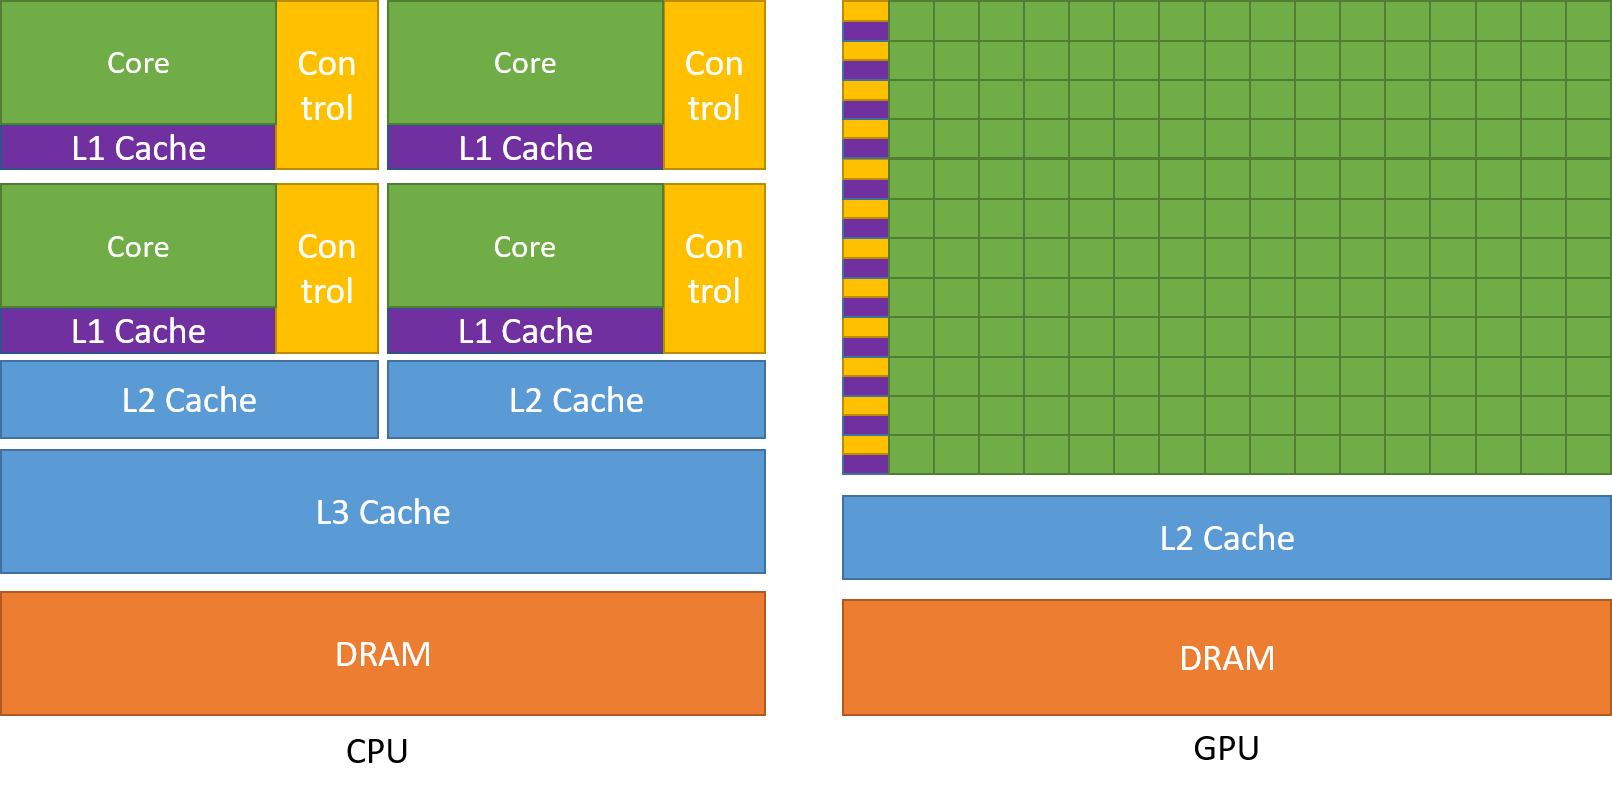
\includegraphics[width=\textwidth]{components/figure/cpu-vs-gpu.png}
  \caption{Comparison of a typical CPU and GPU structure \cite{cudaprog}.}
  \label{figure:cpu-vs-gpu}
\end{figure}

As the staggering performance of a \acrshort{gpu} has not gone unnoticed by the scientific community, work has been done to allow the \acrshort{gpu} to process workloads unrelated to graphics, e.g., linear solvers \cite{cusolver}, or neural networks \cite{cudnn}.

\subsection{Hardware architecture}

As the implementation of both B+Tree and B-Link-Tree is based on CUDA (see Chapter \ref{label:cuda}), we're focusing on NVIDIA \acrshort{gpu} and its architecture in this work. Since the introduction of unified shared architecture with GeForce 8 Series in 2006, a single NVIDIA GPU comprises an array of \textit{streaming multiprocessors} (SM). The power of a single GPU card depends on the number of these streaming multiprocessors, which may vary between models. Each \acrshort{sm} in general have these components:
\begin{itemize}
  \item \textit{Streaming processors}\footnote{Also known as a \textit{CUDA core}}, each containing an arithmetic logic unit (ALU) for integer operations and floating-point unit (FPU) for floating-point operations.
  \item \textit{Register file}, where threads store their local variables. This register file is shared between all threads running in the SM. The number of available registers per thread is defined by architecture.
  \item \textit{Instruction cache}, which caches the instruction without the data for quick fetching.
  \item \textit{Shared memory} used to share data between threads in the same thread block (see Chapter \ref{label:gpu:mem}).
  \item \textit{L1 / Texture cache}, which is used to store local memory of the thread or to serve as a texture cache for image data.
\end{itemize}

Newer architectures include more specialized cores, for example, \textit{tensor cores} in every SP, capable of executing 4x4 matrix multiplication instructions. Or \textit{RT cores} in every SM, accelerating raytracing, found in recent Ampere architecture (see Figure \ref{figure:ampere-sm}).

\begin{figure}[H]
  \centering
  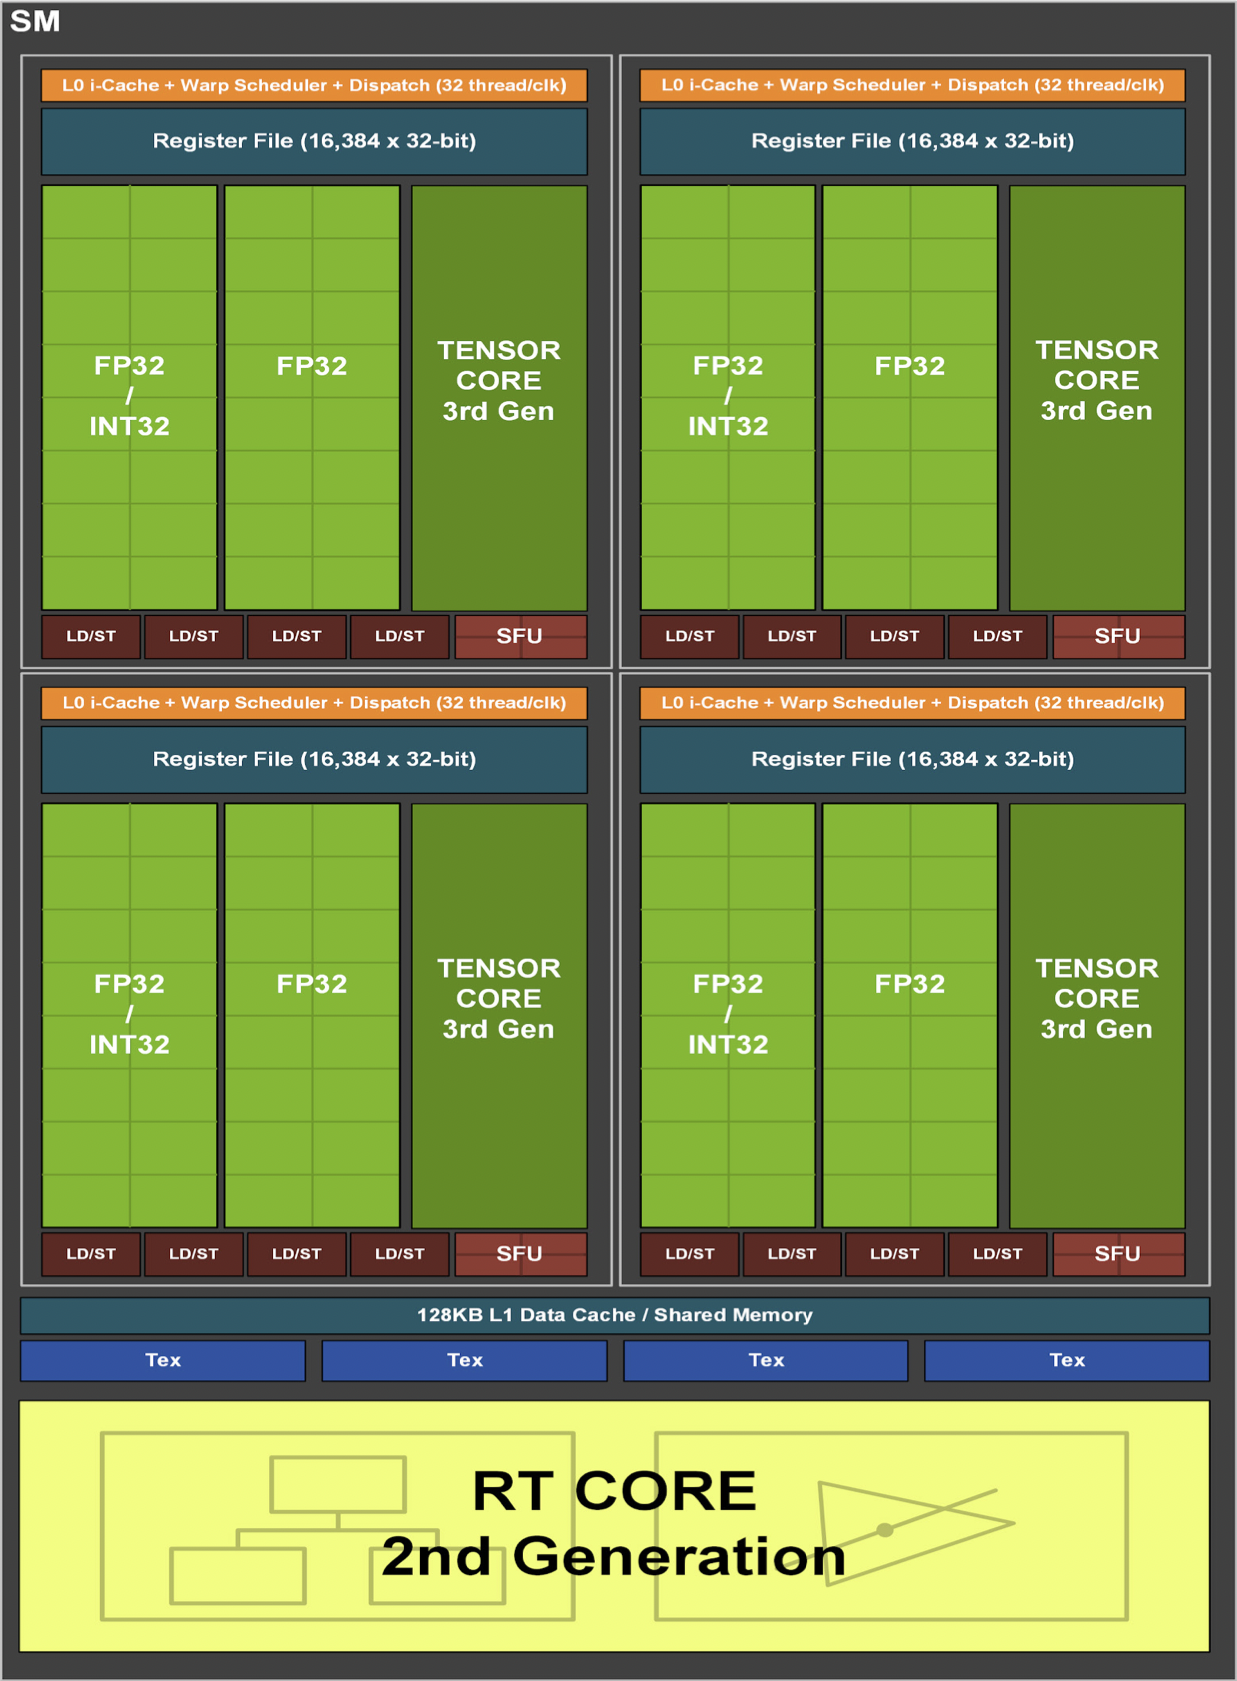
\includegraphics[width=\textwidth]{components/figure/ampere-sm.png}
  \caption{Ampere GA10x Streaming Multiprocessor \cite{nvidiaampere}}
  \label{figure:ampere-sm}
\end{figure}

\subsection{Memory hiearchy} \label{label:gpu:mem}

Each \acrshort{gpu} has its own memory with its memory hierarchy separate from the rest of the system. Every thread has access to its registry and local memory. Local memory is used to store variables for which we do not have space in registers (registry spilling), or we cannot determine if we do have space (like arrays). The registry and the local memory are not directly accessible to the programmer and are managed by the compiler instead.

Each thread also has access to shared memory, which is shared with all threads executing on the same thread block (see Chapter \ref{label:cuda}). As the memory resides on-chip itself, it has higher throughput and lower latency compared to the global memory. It can be considered a user-managed cache, as the application itself takes care of allocation and access to the cache.

Finally, all threads have access to the global memory, available to all threads regardless of the residing multiprocessor. The global memory is the largest memory available on the GPU. But it is also the slowest, as it is stored on a separate chip. Read and writes are done in 32-, 64-, or 128-byte memory transactions \cite{cudaprog}.

Both local and global memory can be routed through L2 and L1 cache. L1 and L2 cache work in a similar manner as in the CPU to speed up memory access. L1 cache level has lower latency than the L2 cache level when accessing, and both of these caches are faster than accessing the memory directly. Thus, to increase memory throughput, it is desirable to store and read data in faster caches than from memory itself -- keeping both cache utilization and hit rate high.

This can be achieved by organizing the memory allocation and access to honor temporal locality, ensuring the duration between the reuse of specific data is as short as possible, and spatial locality, keeping our data access close to each other.


\section{CUDA programming model} \label{label:cuda}

To simplify development on general-purpose GPUs, NVIDIA introduced the \acrfull{cuda} programming model in November 2006. As mentioned previously, GPUs are suited for parallel workloads optimizing in total throughput, sacrificing the performance of serial operations. However, not all programs are fully parallel in nature, and some problems are difficult, if not impossible, to formulate in a manner that would benefit from the use of a GPU. Thus, a sane idea would be to utilize both CPU and GPU, using GPU in workloads, where parallelism yields significant performance uplift. With CUDA, programmers can write applications run on the CPU and accelerate parallel workloads with the GPU while using familiar C/\CC\ programming language for both processors.

In \acrshort{cuda}, the CPU and GPU and their memory are referred to as \textit{host} and \textit{device} respectively. A host manages the memory of both the device and the host itself, and it launches user-defined functions, called \textit{kernels}, which the device executes. A program thus usually executes serial code on the host and parallel code on the device.

\subsection{Thread hiearchy}

Multiple parallel threads execute these kernels on the GPU. These threads are grouped by the programmer or compiler into \textit{thread blocks} and \textit{grids}, which the GPU uses to schedule work. A GPU scheduler maps these abstractions to concrete hardware units: A grid is mapped to a GPU, a thread block is mapped to a \textit{streaming multiprocessor} (SM), and a thread is mapped to a \textit{streaming processor} (SP / CUDA core).

From the implementation side, to launch a kernel function, a programmer must specify the number of threads in a single thread block and the number of thread blocks in a grid. CUDA extends the \CC\ language with \mintinline{cuda}{<<<numBlocks, blockSize>>>} syntax for that purpose.

Every thread in a thread block has an identifier, which is exposed inside the thread as a constant variable: \code{threadIdx}. Similarly, each thread block can be identified with the block index within a grid, \code{blockIdx}. With the dimensions of a block known \code{blockDim}, the global index of a thread can be computed as such:

$$x = blockIdx.x * blockDim.x + threadIdx.x$$

This global index is often used to determine what data is being accessed by a single thread. A programmer may choose to address the threads in a two-, or three-dimensional way instead of a one-dimensional way for the sake of convenience, especially when dealing with matrices or volumes.

\subsection{SIMT architecture}\label{subsection:simt}

Only a few threads from a thread block are executed at once by a streaming multiprocessor. Before execution, the SM schedules threads in a group of 32, called a \textit{warp}. A warp scheduler then picks a warp and executes a single instruction with different data on all threads in a warp. This architecture is called \acrfull{simt}.

All threads in a warp execute the same line of code at once. This rule at face value permits any thread divergence, most notably disallowing the usage of conditionals such as if-else statements. Threads cannot run different branches in parallel, as all threads must run the same instruction simultaneously. As a workaround, divergent branches are executed in series by all threads. Threads not participating in the active execution branch are deactivated while still consuming resources. The cost of execution effectively becomes a sum of the cost of all branches. Generally, warps are at their peak efficiency when all threads run the same code without any branching.

\subsection{Synchronization}

At some point, synchronization needs to happen, either for threads to communicate and share data with each other or to ensure all threads have completed their work at a certain point.

Kernel launches from the host are asynchronous by nature, and the host code will not wait for results unless \codecpp{cudaDeviceSynchronize()} is invoked. This instruction will block the host until the device has completed all preceding requested tasks \cite{cudaprog}.

Threads can also be synchronized, as threads do not execute at the same time and thus do not complete their task simultaneously. A synchronization barrier \codecpp{__syncthreads()} is used to synchronize the threads in a thread block, which all threads must reach to resume execution. This barrier guarantees that all code preceding the instruction is executed before the code after the instruction.

Threads inside a thread block may use shared memory or global memory to cooperate and share data. To ensure all writes to the memory are visible to all other threads, \codecpp{__threadfence()} can be used to stall the threads until writes to the memory are completed.

Warp-level primitives enable fine-tuned collective operations within warps. Parallel reductions and synchronized data exchange can be achieved with \codecpp{__shfl_down()} and \codecpp{__shfl_sync()} respectively. \codecpp{__syncwarp()} can be utilized to create a synchronization barrier for all threads in a warp, similar to the function \codecpp{__syncthreads()} for all threads in a thread block.

At last, atomic functions (such as \codecpp{atomicAdd()} or \codecpp{atomicCAS()}) can be used to read from or write to shared or global memory while ensuring no interference from other threads until the operation is complete.
\section{TNL}

\acrfull{tnl} \cite{tnl} is a \CC\ library offering robust tools for high-performance computing and computational science. The primary goal of this project is to provide a familiar API akin to \code{STL} while offering significant performance uplift by exploiting the parallel nature of GPUs.

The library makes extensive use of template meta-programming to create a unified interface for both \acrshort{cpu} and \acrshort{gpu}, which stays the same regardless of the selected execution target device. This interface allows the programmer to enable or disable invocation on GPU without significant rewrites. This programming pattern heavily influenced the design of the implementation.

\subsection{Views}

Alongside parallelism and contention, the programmer must take care of proper memory management. CUDA only offers low-level primitives for allocating and deallocating memory, similar to languages like C. However, the programmer must also keep in mind the existence of two separate memories. What is allocated on CPUs is directly not accessible from GPUs and vice-versa. Thus, TNL includes classes aiming to alleviate the work needed to address memories between the devices.

\code{TNL::Container::Array} is a template container class for one-dimensional dynamic array. By specifying a type in a template, this class allows the programmer to choose where the data will reside. If the template argument is set to \code{TNL::Devices::Host}, the container behaves similar to \code{std::vector}. However, when the device is set to \code{TNL::Devices::Cuda}, all of the operations are implemented with parallelism in mind.

Data can be directly accessed only from a device where it was previously allocated. To read or write from a different device, copying of data must occur between memories. These cross-device operations are considerably expensive and should thus be used sparingly.

% - One common problem we ought to have is the ability to supply an instance of Array containers. As kernel invocations cannot pass the instance by reference, the contents are copied on GPU, thus creating significant overhead. In order to bypass this issue, a companion class \code{TNL::Container::ArrayView} is provided alongside Array. This class allows the user to read and write data into memory, but forbids allocating or resizing space.
\chapter{Theory}

\section{B-Tree}\label{section:b-tree}

B-Tree is a balanced search tree used for storing large blocks of data. It captures and maintains the sort order of data and supports searching, sequential retrieval, insertion, and deletion in logarithmic time.

Since their invention 50 years ago \cite{bayer-org}, B-Trees have been already considered ubiquitous less than ten years later \cite{10.1145/356770.356776}. They can be found in various forms in databases (e.g., PostgreSQL \cite{postgresql}) and file systems (e.g., btrfs \cite{btrfs}), where a performant self-balancing external index for large blocks of data is required. \todo{Add OLAP, OLTP usages and references}

B-Trees are a specialization of $(a,b)$-Trees, where a B-Tree is either an $(a, 2a)$-tree or $(a, 2a + 1)$-tree depending on the oddness / evenness of $a$. This is also why 2-4 trees (also known as \enquote{2-3-4-trees}) (which in turn are similar to RB-Trees) are B-Trees with an order of 3.

However, it raises why B-Trees are used for on-disk data, and binary search trees are used for in-memory data. The main reason behind this is the high overhead of data access in block-access storage, where byte access is not well supported. A typical example is disk storage, where a disk is divided into blocks. B-Trees exploit this behavior by having its node be as large as a whole block.

B-Trees are exceptionally useful for secondary disk-based storage, but it still yields significant improvements even when storing data in memory; as with CPU caches and memory line caches, we can treat the memory as a block-access device.

The main benefit of B-Trees is their shallow height even with many keys inserted; thus, the number of disk accesses to traverse the tree is also low.

\begin{figure}[H]
  \centering
  \begin{figure}[H]
  \centering
  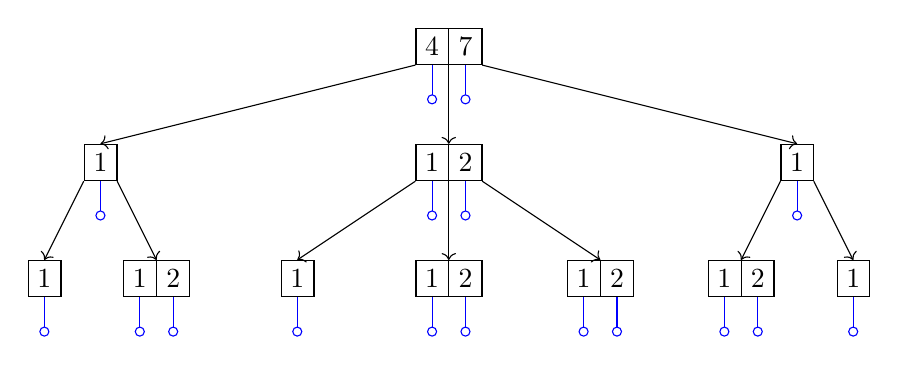
\begin{tikzpicture}[
    bnode/.style = {
        draw,
        rectangle split,
        rectangle split horizontal,
        rectangle split ignore empty parts,
        anchor=north
      },
    bchild/.style = { -> },
    bvalue/.style = { -{Circle[open]}, blue }
    ]

    % Level 0
    \node[bnode](y0) {
      \nodepart{one} $4$ \nodepart{two} $7$
    };

    \draw[bvalue](y0.one south) -- +(0,-0.5);
    \draw[bvalue](y0.two south) -- +(0,-0.5);

    % Level 1
    \draw[bchild](y0.south west) -- +(-4,-1) node[bnode](y1x0){
        \nodepart{one} $1$
      };
    \draw[bvalue](y1x0.one south) -- +(0,-0.5);

    \draw[bchild](y0.one split south) -- +(0,-1) node[bnode](y1x1){
        \nodepart{one} $1$ \nodepart{two} $2$
      };
    \draw[bvalue](y1x1.one south) -- +(0,-0.5);
    \draw[bvalue](y1x1.two south) -- +(0,-0.5);

    \draw[bchild](y0.south east) -- +(4,-1) node[bnode](y1x2){
        \nodepart{one} $1$
      };
    \draw[bvalue](y1x2.one south) -- +(0,-0.5);

    % Level 2
    \draw[bchild](y1x0.south west) -- +(-0.5,-1) node[bnode](y2x0){
        \nodepart{one} $1$
      };
    \draw[bvalue](y2x0.one south) -- +(0,-0.5);

    \draw[bchild](y1x0.south east) -- +(0.5,-1) node[bnode](y2x1){
        \nodepart{one} $1$ \nodepart{two} $2$
      };
    \draw[bvalue](y2x1.one south) -- +(0,-0.5);
    \draw[bvalue](y2x1.two south) -- +(0,-0.5);

    % ------
    \draw[bchild](y1x1.south west) -- +(-1.5,-1) node[bnode](y2x2){
        \nodepart{one} $1$
      };
    \draw[bvalue](y2x2.one south) -- +(0,-0.5);

    \draw[bchild](y1x1.one split south) -- +(0,-1) node[bnode](y2x3){
        \nodepart{one} $1$ \nodepart{two} $2$
      };
    \draw[bvalue](y2x3.one south) -- +(0,-0.5);
    \draw[bvalue](y2x3.two south) -- +(0,-0.5);

    \draw[bchild](y1x1.south east) -- +(1.5,-1) node[bnode](y2x4){
        \nodepart{one} $1$ \nodepart{two} $2$
      };
    \draw[bvalue](y2x4.one south) -- +(0,-0.5);
    \draw[bvalue](y2x4.two south) -- +(0,-0.5);

    % ------
    \draw[bchild](y1x2.south west) -- +(-0.5,-1) node[bnode](y2x5){
        \nodepart{one} $1$ \nodepart{two} $2$
      };
    \draw[bvalue](y2x5.one south) -- +(0,-0.5);
    \draw[bvalue](y2x5.two south) -- +(0,-0.5);

    \draw[bchild](y1x2.south east) -- +(0.5,-1) node[bnode](y2x6){
        \nodepart{one} $1$
      };
    \draw[bvalue](y2x6.one south) -- +(0,-0.5);

  \end{tikzpicture}
  \caption{B-Tree with $\mathit{Order} = 3$}
\end{figure}

  \caption{B-Tree with $\mathit{Order} = 3$.}
\end{figure}

\begin{definition}\label{def:btree}
  B-Tree of order $m$ is a rooted tree with following properties:
  \begin{enumerate}
    \item Every node $x$ has following attributes:
          \begin{enumerate}
            \item $x.\mathit{size}$, the number of keys in a node,
            \item $x.\mathit{leaf}$, a boolean value indicating whether the node is a leaf or not,
            \item An list of $x.\mathit{size}$ keys $x.\mathit{key}_1, x.\mathit{key}_2, \dots, x.\mathit{key}_{x.size}$ sorted in ascending order ($x.\mathit{key}_1 \le x.\mathit{key}_2 \le \dots \le x.\mathit{key}_{x.\mathit{size}}$),
          \end{enumerate}
    \item Every internal node $x$ has $x.size + 1$ pointers as its children \\($x.child_1, x.child_2, \dots, x.child_{x.size + 1}$),
    \item All leaf nodes appear at the same depth, which is the height of tree $h$,
    \item Nodes have upper and lower bounds, which limit the number of keys and children. Assuming $m$ is the order of a B-Tree:
          \begin{enumerate}
            \item Every node other than the root has at least $\floor{\nicefrac{m}{2}}$ children, thus every node other than root has at least $\floor{\nicefrac{m}{2}} - 1$ keys,
            \item The root node has at least two children, except if it is a leaf node,
            \item Every node may contain at most $m$ children, thus may contain at most $m - 1$ keys.
          \end{enumerate}
  \end{enumerate}
\end{definition}

\begin{lemma}
  B-Tree $T$ of order $m$ with $n \ge 1$ keys has height $h = \Theta(\log{n})$.
\end{lemma}

\begin{proof}
  Assume $t = \floor{\nicefrac{m}{2}}$ as the minimum number of children in a node. The root of $T$ has at least one key; all other nodes contain at least $t - 1$ keys.

  Thus, $T$ has at level $1$ at least $2$ nodes, at level $2$ at least $2t$ nodes, and so forth. The last level $h$ will have at least $2t^{h-1}$ nodes.

  Define $n_{min}$ as the minimum amount of keys in $T$ of height $h$ as the sum of key count per depth.

  \begin{equation}
    \begin{split}
      n_{min} & = 1 + (t - 1) \cdot (2 + 2t + \dots + 2t^{h-1}) \\
      &= 1 + 2 \cdot (t - 1) \cdot \sum^{h}_{i = 1}{t^{i-1}} = 1 + 2 \cdot (t - 1) \cdot \sum^{h - 1}_{i = 0}{t^{i}} \\
      &= 1 + 2 \cdot (t - 1) \cdot (\frac{t^h - 1}{t - 1}) = 2t^h - 1
    \end{split}
  \end{equation}

  The maximum amount of keys at height $h$ is defined similarily:

  \begin{equation}
    \begin{split}
      n_{max} & = (m - 1) \cdot \sum^{h - 1}_{i = 0}{m^i} \\
      &= (m - 1) \cdot (\frac{m^h - 1}{m - 1}) = m^h - 1
    \end{split}
  \end{equation}

  As $n_{min} \le n \le n_{max}$, taking logarithm will prove the theorem.
\end{proof}

As search, insertion, and deletion on a single node takes $\Theta{(1)}$, time complexity of every operation is $\Theta{(\log{n})}$. The space complexity for B-Tree is $\Theta{(n)}$.

\subsection{Search}

The search algorithm for B-Trees is trivial but crucial, similar to the search algorithm for binary search trees. We compare the keys in every node and decide the subtree to continue the search starting from the root node, as seen in lines 3--4 in the sample \cref{alg:b-tree-search}. The search ends if we find the desired key or if we end up in a leaf node, which does not have any children.

\begin{algorithm}
  \caption{B-Tree Search}\label{alg:b-tree-search}
  \SetKwInOut{Input}{Input}
  \SetKwInOut{Output}{Output}
  \DontPrintSemicolon

  \SetKwFunction{Search}{Search}
  \SetKwFunction{UpperBound}{UpperBound}

  \SetKwProg{Fn}{Function}{:}{}
  \Fn{\Search{$node$, $needle$}}{
    $i \gets 0$\;

    \While{$i < node.size$ $\&\&$ $needle > node.key_i$}{
      $i \gets i + 1$\;
    }

    \If{$node.key_i$ = $needle$}{
      \KwRet{$($$node$, $i$$)$}\;
    }

    \If{node.leaf = \textbf{true}}{
      \KwRet{null}\;
    }

    \KwRet \Search{$node.child_i$, $needle$}\;
  }
\end{algorithm}

Line 3--4 in the sample \cref{alg:b-tree-search} can be replaced with a binary search or parallelized search in CUDA, which is more suited towards SIMD systems.

\subsection{Insertion}

First, we traverse the tree for the existence of the key. The algorithm will end up in a leaf node if the key is not found. Thus, we need to add the key to the parent of the found node

If a node after insertion has subsequently become full after insertion, a split operation must occur to preserve the rules of the B-Tree \cref{def:btree}. The node is considered \textit{full} if the node contains exactly $m - 1$ keys. The median key is chosen as the separator, and the node is split into two smaller nodes based on that separator. The separator is inserted into the parent of the split node, which might trigger the split operation again.

When the root node needs to be split, a new node with the separator as its only key and two subtrees as its children, which the definition \cref{def:btree} permits (only internal nodes must contain at least $\floor{\nicefrac{m}{2}}$ keys).

\subsection{Deletion}

Deletion in B-Trees is analogous to insertion. We start by searching the tree for the desired key.

If the key is found on a leaf node, we can trivially delete the key from the node. If the node has subsequently become \textit{underfull} by not containing at least $\ceil{\nicefrac{m}{2}}$ keys, the tree must be rebalanced.

Deleting a key from an internal node is more complicated, as child nodes are bound to keys, and a key deletion will result in the loss of a child. Thus, instead of deleting, we swap the key with a successor (or predecessor) key. The key can then be deleted as it is located in a leaf node after the swap. Similar rebalancing must occur if the node has become underfull.

Rebalancing of node $x$ is performed when $x.size = \floor{\nicefrac{m}{2}} - 1$. Assume, without loss of generality, a sibling node $l$ on the left of $x$ exists, and $i$ is the key, which binds the node $n$ to its parent. If a left sibling does not exist or does not have any spare keys to share, a right sibling is used instead, and the rebalancing operation is mirrored.

If the sibling node $l$ has at least $\floor{\nicefrac{m}{2}} + 1$ keys, we can perform the borrowing operation; the key $i$ is prepended to the node $x$ and the last key of $l$ detaches from $l$ and replaces the key $i$. Last child of $l$ is also detached and prepended to $x$.

However, if neither the sibling nodes have enough keys, a merge operation occurs. Both the $x$ node and its sibling $l$ are deleted, and a new node is created instead. This new node contains keys and children of both $x$ and $l$, with key $i$ in the middle. Deletion is, thus, propagated upwards. In the event of a root with no keys and a single child, the single child becomes the new root.

Many implementations forgo rebalancing the tree in favor of replacing the key with a tombstone \cite{goetz-tech}. The tombstone is useful even when inserting, as a key could be directly inserted in place of a tombstone if applicable, thus alleviating the cost of inserting a new key into a sorted list. Rebalancing the tree can be postponed and executed later.


\section{B$^+$Tree}

\begin{definition}
  B$^+$Tree is a B-Tree where keys are stored exclusively in leaf nodes.
\end{definition}

Separators found in internal nodes can be freely chosen and may not match the actual keys in leaf nodes, as long as these separators split the tree into subtrees and preserve the ordering of the keys.

As the B$^+$Tree does not reuse the keys and may duplicate the keys found in the leaf nodes to use as separators in internal nodes, they do bear increased storage requirements. Compressing techniques on keys can be used to reduce the increased space complexity in exchange for increased complexity caused by compressing itself.

In most implementations, leaf nodes may include an additional pointer to a right sibling node, enabling straightforward sequential querying, which is helpful for range querying.

\begin{figure}[H]
  \centering
  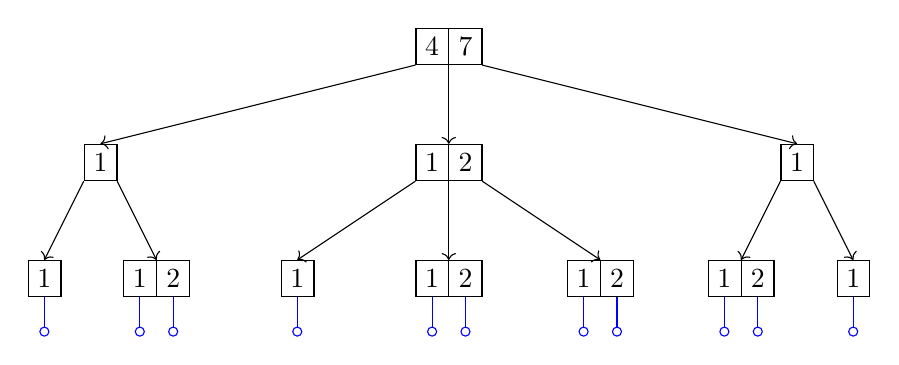
\begin{tikzpicture}[
    bnode/.style = {
        draw,
        rectangle split,
        rectangle split horizontal,
        rectangle split ignore empty parts,
        anchor=north
      },
    bchild/.style = { -> },
    bvalue/.style = { -{Circle[open]}, blue }
    ]

    % Level 0
    \node[bnode](y0) {
      \nodepart{one} $4$ \nodepart{two} $7$
    };

    % Level 1
    \draw[bchild](y0.south west) -- +(-4,-1) node[bnode](y1x0){
        \nodepart{one} $1$
      };

    \draw[bchild](y0.one split south) -- +(0,-1) node[bnode](y1x1){
        \nodepart{one} $1$ \nodepart{two} $2$
      };

    \draw[bchild](y0.south east) -- +(4,-1) node[bnode](y1x2){
        \nodepart{one} $1$
      };

    % Level 2
    \draw[bchild](y1x0.south west) -- +(-0.5,-1) node[bnode](y2x0){
        \nodepart{one} $1$
      };
    \draw[bvalue](y2x0.one south) -- +(0,-0.5);

    \draw[bchild](y1x0.south east) -- +(0.5,-1) node[bnode](y2x1){
        \nodepart{one} $1$ \nodepart{two} $2$
      };
    \draw[bvalue](y2x1.one south) -- +(0,-0.5);
    \draw[bvalue](y2x1.two south) -- +(0,-0.5);

    % ------
    \draw[bchild](y1x1.south west) -- +(-1.5,-1) node[bnode](y2x2){
        \nodepart{one} $1$
      };
    \draw[bvalue](y2x2.one south) -- +(0,-0.5);

    \draw[bchild](y1x1.one split south) -- +(0,-1) node[bnode](y2x3){
        \nodepart{one} $1$ \nodepart{two} $2$
      };
    \draw[bvalue](y2x3.one south) -- +(0,-0.5);
    \draw[bvalue](y2x3.two south) -- +(0,-0.5);

    \draw[bchild](y1x1.south east) -- +(1.5,-1) node[bnode](y2x4){
        \nodepart{one} $1$ \nodepart{two} $2$
      };
    \draw[bvalue](y2x4.one south) -- +(0,-0.5);
    \draw[bvalue](y2x4.two south) -- +(0,-0.5);

    % ------
    \draw[bchild](y1x2.south west) -- +(-0.5,-1) node[bnode](y2x5){
        \nodepart{one} $1$ \nodepart{two} $2$
      };
    \draw[bvalue](y2x5.one south) -- +(0,-0.5);
    \draw[bvalue](y2x5.two south) -- +(0,-0.5);

    \draw[bchild](y1x2.south east) -- +(0.5,-1) node[bnode](y2x6){
        \nodepart{one} $1$
      };
    \draw[bvalue](y2x6.one south) -- +(0,-0.5);

  \end{tikzpicture}
  \caption{B$^+$Tree with $\mathit{Order} = 3$}
\end{figure}


All operations on the B$^+$Tree are simplified thanks to storing the keys exclusively in leaf nodes, as the end state when traversing a tree is always a leaf node.

Tree rebalancing operations in B$^+$Tree, such as splitting full nodes and merging free nodes, are the same as in B-Tree, with the only difference is the removal of the median key in leaf nodes. The median key is only propagated to the parent node after a split; the key itself is preserved in the leaf node, ensuring the rules of B$^+$Tree are not broken.
\section{Concurrency Control}

The primary goal of concurrency control is to ensure the correctness of results after concurrent operations are performed on the structure. Concurrency control can mean two things, either the correctness and serializability of logical contents or serializability among threads modifying data structure in memory.

In databases, the primary concern is to protect database contents, regardless of the internal representation of said contents. Locks are utilized to separate concurrent transactions. These locks have sophisticated acquiring and releasing mechanisms, usually handled by a lock manager with the support of prioritization and queuing. As these locks ensure the serializability of database contents but not their representation, a B-Tree does not require locks of all non-leaf pages.

In our case, we must ensure the operations modifying the data structure in memory are serializable and do not create an invalid or incomplete state of the entire tree, not just its contents. Latches are commonly used, resembling critical sections implemented by mutexes and semaphores. They have the benefit of lower overhead, as these can be implemented with a handful of instructions in comparison to full-fledged lock managers.

More specifically, splitting a full node is a major challenge for concurrent updates of B-Trees. As one thread is splitting a full B-Tree node, all the other threads must not observe any intermediate or incomplete state of data structure. Two latches on different levels must be acquired to atomically serialize changes to the split node, its new sibling, and the parent of a said split node. Even so, a splitting might propagate towards the root, as a split operation might cause the parent node to subsequently become full, further bottlenecking the concurrency on the entire tree.

Previous approaches include locking a subtree of highest affected node \cite{samadi1976b}, which, albeit straightforward, severely reduced concurrency.

In order to alleviate the bottleneck without risking inconsistency, \textit{B-Link-Tree} relaxes the definition of B-Trees. As explained by Graefe \cite{goetz-tech}:

% \begin{definition}[B-Link-Tree]
%   B-Link-Tree divides node splitting into two independent steps: splitting the node and inserting a new separator key in the parent node. Each node thus has a pointer a sibling at the same level of the tree.
% \end{definition}
\section{B-Link-Tree}\label{section:b-link-tree}

Previous approaches include locking a subtree of highest affected node \cite{samadi1976b}, which, albeit straightforward, reduced concurrency. To alleviate the bottleneck without risking inconsistency, \textit{B-Link-Tree} relaxes the definition of B$^+$Trees. As explained by Graefe \cite{goetz-tech}:

\begin{definition}
  B-Link-Tree is a B$^+$Tree with following properties:
  \begin{enumerate}
    \item Each node $x$ has additional attributes:
          \begin{itemize}
            \item $x.sibling$, a pointer to a right sibling node at the same level,
            \item $x.highkey$, the upper bound of all keys found in the subtree rooted by $x$ (every key found in $x$ is less then $x.highkey$).
          \end{itemize}
    \item Does not require locks nor latches for reading.
  \end{enumerate}
\end{definition}

\begin{figure}[H]
  \centering
  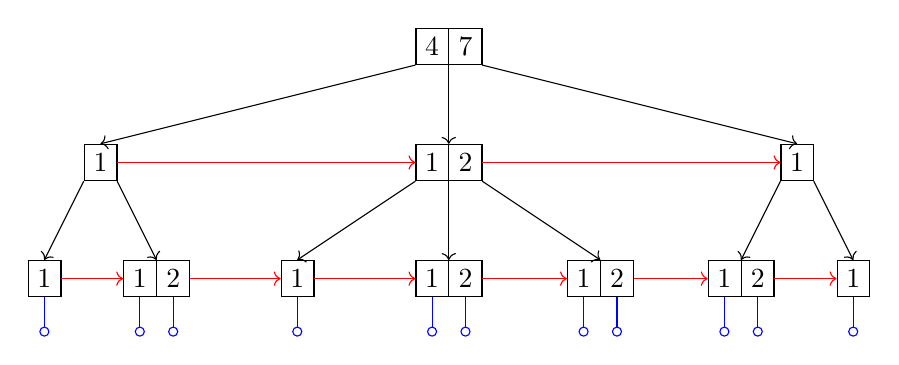
\begin{tikzpicture}[
    bnode/.style = {
        draw,
        rectangle split,
        rectangle split horizontal,
        rectangle split ignore empty parts,
        anchor=north
      },
    bchild/.style = { -> },
    bsibling/.style = { ->, red },
    bvalue/.style = { -{Circle[open]}, blue }
    ]

    % Level 0
    \node[bnode](y0) {
      \nodepart{one} $4$ \nodepart{two} $7$
    };

    % Level 1
    \draw[bchild](y0.south west) -- +(-4,-1) node[bnode](y1x0){
        \nodepart{one} $1$
      };

    \draw[bchild](y0.one split south) -- +(0,-1) node[bnode](y1x1){
        \nodepart{one} $1$ \nodepart{two} $2$
      };

    \draw[bchild](y0.south east) -- +(4,-1) node[bnode](y1x2){
        \nodepart{one} $1$
      };

    \draw[bsibling](y1x0.east) -- (y1x1.west);
    \draw[bsibling](y1x1.east) -- (y1x2.west);

    % Level 2
    \draw[bchild](y1x0.south west) -- +(-0.5,-1) node[bnode](y2x0){
        \nodepart{one} $1$
      };
    \draw[bvalue](y2x0.one south) -- +(0,-0.5);

    \draw[bchild](y1x0.south east) -- +(0.5,-1) node[bnode](y2x1){
        \nodepart{one} $1$ \nodepart{two} $2$
      };
    \draw[bvalue](y2x1.one south) -- +(0,-0.5);
    \draw[bvalue](y2x1.two south) -- +(0,-0.5);

    % ------
    \draw[bchild](y1x1.south west) -- +(-1.5,-1) node[bnode](y2x2){
        \nodepart{one} $1$
      };
    \draw[bvalue](y2x2.one south) -- +(0,-0.5);

    \draw[bchild](y1x1.one split south) -- +(0,-1) node[bnode](y2x3){
        \nodepart{one} $1$ \nodepart{two} $2$
      };
    \draw[bvalue](y2x3.one south) -- +(0,-0.5);
    \draw[bvalue](y2x3.two south) -- +(0,-0.5);

    \draw[bchild](y1x1.south east) -- +(1.5,-1) node[bnode](y2x4){
        \nodepart{one} $1$ \nodepart{two} $2$
      };
    \draw[bvalue](y2x4.one south) -- +(0,-0.5);
    \draw[bvalue](y2x4.two south) -- +(0,-0.5);

    % ------
    \draw[bchild](y1x2.south west) -- +(-0.5,-1) node[bnode](y2x5){
        \nodepart{one} $1$ \nodepart{two} $2$
      };
    \draw[bvalue](y2x5.one south) -- +(0,-0.5);
    \draw[bvalue](y2x5.two south) -- +(0,-0.5);

    \draw[bchild](y1x2.south east) -- +(0.5,-1) node[bnode](y2x6){
        \nodepart{one} $1$
      };
    \draw[bvalue](y2x6.one south) -- +(0,-0.5);

    \draw[bsibling](y2x0.east) -- (y2x1.west);
    \draw[bsibling](y2x1.east) -- (y2x2.west);
    \draw[bsibling](y2x2.east) -- (y2x3.west);
    \draw[bsibling](y2x3.east) -- (y2x4.west);
    \draw[bsibling](y2x4.east) -- (y2x5.west);
    \draw[bsibling](y2x5.east) -- (y2x6.west);

  \end{tikzpicture}
  \caption{B-Link-Tree with $\mathit{Order} = 3$}
\end{figure}


Splitting during node insertion is divided into two independent steps:  \textit{splitting a node} and inserting the split node with its new separator key to the parent node.

When splitting node $x$, a new right sibling node $y$ is created. The node $y$ inherits the high key from the split node $x$, whereas the first key of $y.keys$ is used as a new $x.highkey$. Thus, an internal node does exist without a parent in between the operations. $x.highkey$ is used to be able to traverse the newly split node and its subtree, even when the split operation is not complete.

As the final step of node splitting, the separator key and the newly split node $y$ are inserted in the parent node. Similar to the insertion in B-Tree, a split operation might trigger additional splitting in higher levels.

Tree traversal is modified to honor $x.highkey$ by returning the node at $x.sibling$ when the target key $k$ is larger or equal than $x.highkey$.

\subsection{Proof of correctness}

To prove the correctness of each operation performed on the B-link-tree, the following theorems need to be proven:

\begin{itemize}
  \item \textit{Deadlock freedom} -- threads performing operations on the B-link-tree cannot produce a deadlock,
  \item \textit{Correct tree modifications} -- the tree must appear as a valid tree for all nodes at any time,
  \item \textit{Correct interactions} -- concurrent operations do not interfere with one another.
\end{itemize}

\begin{theorem}
  \textit{Deadlock freedom} -- threads performing operations on the B-link-tree cannot produce a deadlock.
\end{theorem}

\begin{proof}
  By imposing a total ordering of nodes, cycles are eliminated from the system and thus the system is deadlock free.

  To prove a total ordering of nodes, the following ordering $a < b$, where $a$ and $b$ are nodes of the tree, is considered:

  \begin{enumerate}
    \item If $a$ and $b$ are not on the same distance from the root node, then $a < b$ if and only if node $a$ is less distant from root node than node $b$ (bottom-up).
    \item If $a$ and $b$ are on the same level, then $a < b$ if and only if node $b$ is reachable from node $a$ by following a chain of one or more $sibling$ pointers (left-to-right).
  \end{enumerate}

  It can be shown that during insertion operation the total ordering of nodes is preserved. If $a < b$ at time $t_0$ at the start of insertion, then $a < b$ is preserved for $\forall t, t > t_0$, as a node $x$ during split operation will create a node $x^\prime$ and $x^{\prime\prime}$, where $x^\prime < x^{\prime\prime}$ and:

  $$\forall y, y < x \Leftrightarrow y < x^\prime$$
  $$\forall y, x < y \Leftrightarrow x^{\prime\prime} < y$$

  Therefore, insertion will not break the total ordering of nodes.

  Latches for the nodes are acquired by following the ordering; thus once a latch is acquired for a node, no other latch will be acquired on any node below it, nor on any node on the same level.
\end{proof}

\begin{theorem}\label{theorem:b-link-tree:modifications}
  \textit{Correct tree modifications} -- the tree must appear as a valid tree for all nodes at any time.
\end{theorem}

\begin{proof}
  The tree must appear as a valid tree for all threads at any time except for the modifying thread. Assuming writing is done by invoking $writeNode$ function, which will write to the storage atomically.

  The insertion operation, assuming performed on a node $x$ of the tree, will therefore write only in these circumstances:

  \begin{enumerate}
    \item $writeNode(x)$ -- if node $x$ is not considered full and is safe for rewriting,
    \item $writeNode(x^\prime)$ -- writing a newly allocated node $x^\prime$, which was created in the process of splitting node $x$,
    \item $writeNode(x)$ -- rewriting the node $x$ as part of the splitting process, $x.sibling$ is set to point at node $x^\prime$.
  \end{enumerate}

  Even though $writeNode(x^\prime)$ and subsequent $writeNode(x)$ operation are done in two writes, it can be shown, that these operations are equivalent to a single change in tree structure:

  \begin{itemize}
    \item When $writeNode(x^\prime)$ is executed, no other node has a pointer at $x^\prime$. Therefore this operation will not modify the tree structure,
    \item when $writeNode(x)$ is subsequently executed, the $x.sibling$ is set to point to $x^\prime$. This operation therefore does both modify the node $x$ and introduce newly allocated node $x^\prime$ to the tree in a single operation.
  \end{itemize}
\end{proof}

\begin{theorem}
  \textit{Correct interactions} -- concurrent operations do not interfere with one another.
\end{theorem}

\begin{proof}
  Assume $t_i$ is the time when the insertion process $I$ writes node $x$ to storage, and $t_r$ is the time when another operation $P$ reads the same node $x$. All of the operations are considered atomic, thus $t_i \neq t_r$.

  First, the case of $t_r > t_i$, where an operation $P$ is reading a node $x$ later than the insertion, is completed is considered; any changes that the insertion process $I$ does will preserve the correct tree structure, as proven in Theorem \ref{theorem:b-link-tree:modifications}.

  In the case of $t_r < t_i$, where insertion $I$ happens after operation $P$ does a read. the proof is broken into three possible scenarios, which the insertion might perform:

  \begin{enumerate}
    \item Simple insertion of a key-pointer pair into node $x$ without splitting,
    \item splitting of node $x$, where the inserted key is placed in the left node $x$, same as the node, which has been split,
    \item splitting of node $x$, where the inserted key is placed in the right node $y$, the newly allocated node.
  \end{enumerate}

  In the first scenario, $I$ performs the insertion in node $x$ without additional splitting. If it is inserting into a leaf node ($x.leaf = true$), no other pointers are inserted by the process $I$, and the operation $P$ behaves as if the read happened before insertion.

  If the insertion happens on an internal node ($x.leaf = false$), a key-pointer pair created by splitting a lower-level node $z$ is inserted into the node $x$. As the node $z$ has already been split, as this is the only situation where a key-pointer pair could propagate upwards to node $x$, the operation $P$ will be able to utilize the link pointers $z.sibling$ to reach both the original node and the newly split node.

  In the second and third scenarios, the process $I$ has split the node $x$ into two nodes $x_1$ and $x_2$. If the process is happening on leaf nodes, $P$ will continue as if no insertion has occurred. In non-leaf nodes, a key-pointer pair from the newly split node from the lower level is inserted into node $x$, which caused the node to be split. Both the insertion and search in the node below node $x$ will be correct thanks to Theorem \ref{theorem:b-link-tree:modifications}. It only remains to prove the correctness of split operation on node $x$.

  Assume $z$ is the node, which has been created by splitting a node below $x$ and $z_l$ the node on the left of node $z$ ($z_l.sibling = z$).
  If the search would not follow the pointer of $z$, the operation $P$ will proceed as usual because the nodes $x_1$ and $x_2$ contain the same set of pointers as node $x$ with the addition of the pointer to $z$. Otherwise, if the search would follow the pointer to $z$, had the process $P$ read the node $x$ after the split, the operation $P$ will proceed instead to the node left of the node $z$, $z_l$. The operation $P$ is then able to reach node $z$ by using the link pointer of node $z_l$.

  If the process $P$ is another insertion process, it is either searching for the correct node, backtracking upwards, or attempting to insert into node $x$. In the case of searching, the proof is the same as if the process $P$ was a search operation.

  In the case of backtracking, the node $n$ might have been split multiple times since the last read when traversing downwards in the search operation. In this scenario, the insertion process will find the proper target node for insertion using link pointers, as the order between nodes is preserved, and the newly split nodes of node $n$ will be found on the right side of node $n$.

  Finally, the process $P$ can attempt to insert a key (or a key-pointer pair) into node $n$. In this scenario, only one process can hold a latch for the node $n$. After the latch has been acquired by one of the insertion processes, the other will attempt to read the node $n$ afterward. As the read occurs after write, Theorem \ref{theorem:b-link-tree:modifications} proves this interaction to be correct.

\end{proof}


\chapter{Realisation}\label{chapter:realisation}

In this chapter, implementation details and design choices made to construct a B-Tree implementation on GPU are presented. The entire implementation is written in \acrshort{cuda} \CC\ with the usage of \acrshort{tnl}.

\section{Warp Cooperative Work Sharing strategy}

Warp-cooperative work-sharing strategy (WCWS) is used to improve the performance of each operation by exploiting the behavior of NVIDIA GPUs and how threads are executed in each SM. As SMs have a limited number of cores, threads are organized into groups of 32 threads called \textit{warps} (see Chapter \ref{label:cuda}).

As threads can communicate with each other in a warp using warp-wide communication primitives in CUDA, these threads can synchronize with each other and work on a single task.

This strategy is thoroughly used in all of our B-Tree operations, especially during updates. We can achieve better memory coalescing and unlock vector load and stored by utilizing every thread in a warp. As a side effect, the order of a B-Tree is upper bound by the number of threads available in a warp, which is 32 in contemporary GPUs.
 
\todo{Add pseudocode explaining WCWS}
\section{Warp-based operations}

As discussed in \cref{section:wcws}, both GPU implementations use the WCWS strategy, and all threads of a warp are cooperating to process a single task. Whether it is an insertion, removal, or query operation, thus, it does make sense to use this implementation detail to speed up commonly used, performance-critical computations.

One such computation is finding the correct key index in a node, whether to find a specific key in a leaf node or to find the right child node to traverse into the correct sub-tree. This computation essentially boils down to finding the index of a lower and upper bound key, the former being the first key in a node that is greater or equal to a searched key, the latter being the first node key greater than a searched key.

\begin{algorithm}
  \caption{Lower bound in sorted list}\label{alg:lower-bound}
  \DontPrintSemicolon

  \KwIn{$keys[0\dots{n}], needle$}
  \KwResult{Position of a lower bound key}

  \textit{index} $\gets$ 0, \textit{size} $\gets$ n\;
  \While{size $>$ 0}{
    $step \gets size / 2$\;
    $it \gets index + step$\;
    \eIf{$keys[it] < needle$}{
      $index \gets it + 1$\;
      $size \gets size - step + 1$\;
    }{
      $size \gets step$\;
    }
  }
  \KwRet{index}\;
\end{algorithm}

On the host implementation, the lower-bound key is found by performing a binary search, as the keys are stored in a sorted manner in each node, thus allowing a search with time complexity $\mathcal{O}(\log_2 n)$. Implementation of a lower bound function can be seen in \cref{alg:lower-bound}. However, as all 32 threads perform a single task in a warp, a binary search is sub-optimal on the GPU, as it will inherently execute in series for the reasons of thread divergence, explained in \cref{subsection:simt}.

\begin{listing}
  \begin{minted}{cpp}
__device__ static uint32_t lowerBound(
  KeyType *keys, uint32_t size, KeyType needle
) {
  using cg = cooperative_groups;
  auto threadBlock = cg::this_thread_block();
  auto warp = cg::tiled_partition<32>(threadBlock);

  uint64_t rank = warp.thread_rank();
  uint32_t ballot = warp.ballot(keys[rank] >= needle);
  uint32_t idx = __ffs(ballot) - 1;

  asm("min.u32 %0, %1, %2;" : "=r"(idx) : "r"(idx), "r"(size));
  return idx;
}
  \end{minted}
  \caption{A warp-friendly implementation of finding a lower-bound key.}
  \label{lst:lower-bound-cuda}
\end{listing}

Thus, it is more efficient to break down the work for every thread to be able to participate, seen in a lower-bound example in \cref{lst:lower-bound-cuda}. A lower bound (and upper bound) search is done as follows: each thread in a warp will read a key from a node and perform a comparison. The results are aggregated as a bitmap using \codecpp{warp.ballot()}, where $N$-th bit indicates whether a thread at index $N$ fulfills the comparison (see line 9). The position is obtained by invoking \codecpp{__ffs} on line 10, which returns the index of a first thread with a fulfilled comparison.

The resulting position must not be greater or equal to the size of a processed node, as reading keys outside the expected node size is undefined behavior. As the data type of a variable storing the position is independent of the used data type for keys or values, a single \code{asm} statement on line 12 is used to clamp the position. This optimization was done specifically to enforce the compiler to use a single \mintinline{asm}{min.u32} statement rather than generating branch and jump statements, thus reducing the number of cycles spent on these critical sections.

This optimization does bring an additional constraint to the structure of a B-Tree node: the $Order$ of a tree must not exceed the number of threads available in a single warp, as if it does, some keys will become inaccessible.

\section{Proactive Splitting}

As specified in Algorithm \ref{alg:b-tree-insert} and Algorithm \ref{alg:b-tree-delete}, we first traverse to the node to perform the node update, and any potential balancing is performed in a bottom-up manner. In our implementation, we decided to opt-in to the top-down approach by splitting any full nodes directly when traversing.

With this approach, we are not required to preserve a stack of parent nodes, as we are guaranteeing every operation will update nodes in at most two depths. \todo{Add proof}. Nodes are split more often and prematurely as a trade-off.
\section{Latching and Concurrency Control}

For our implementation of B-Trees, an additional attribute $x.writelock$ is used to prevent multiple threads from writing to the same node at the same time.

In the B$^+$Tree implementation of insertion, traversal is prevented if encountering a node with a write lock to ensure data serializability, as the node with a lock is most likely not in a correct state and may lead the traversal operation to an incorrect subtree. Thus, to solve this issue, the search is restarted from the start if reaching a node with a lock, sharing the the properties of a back-off lock.

B-Link-Tree has this limitation lifted, as the tree is always traversable, even if the node is locked for writing. As described in Section \ref{section:b-link-tree}, each node has a $x.sibling$ pointer referencing next at the same depth. At every depth, the nodes are essentially chained in a linked list. With this addition, a correct node is always found with the help of the additional path to reach every node.

In both of the implementations, \code{warp.sync()} and \code{\_\_threadfence} is sporadically needed to ensure correct order of instructions used for memory access.
\section{Bulk Insert}

As described by Graefe \cite{goetz-tech}, there is a strong relationship between B-Trees and sorting, which we can utilize. Optimal construction of B-Tree shall forgo incremental insertion in favor of building the tree from a presorted list.

As both B-Link-Tree and B$^+$Tree internally store their key-value pairs in their nodes, incremental insertion can be avoided. Instead, the tree can be constructed in a bottom-up approach, creating all nodes of each level one by one. Sample pseudocode can be seen in \cref{alg:bulk-loading}.

\begin{algorithm}[H]
  \KwIn{\textit{inputKeys}: list of keys to be stored \newline \textit{inputValues}: list of values, each one is bound to a key}
  \DontPrintSemicolon

  $(\mathit{keys}, \mathit{values}) \gets \mathit{sortByKey}(\mathit{inputKeys}, \mathit{inputValues})$\;

  $\mathit{nodeCount} \gets \text{calculate}\ \mathit{nodeCount}$\;

  $(\mathit{keys}, \mathit{children}) \gets \mathit{createLeafKernel}(\mathit{keys}, \mathit{values})$\;

  \While{$\mathit{children}.\mathit{len}() > 1$}{
    $(\mathit{keys}, \mathit{children}) \gets \mathit{createInternalKernel}(\mathit{keys}, \mathit{children})$\;
  }
  $\textit{root} \gets \textit{children}[0]$\;
  \caption{Bulk Insert}
  \label{alg:bulk-loading}
\end{algorithm}

First, the key-value pairs are sorted by key using the built-in \codecpp{thrust::sort} function, as \acrshort{tnl} does not have a sort method yet. Sorted pairs are passed to the \code{createLeafKernel}, which will divide the pairs and fit them into nodes. A fixed offset is chosen to make sure each node is not immediately full.
The expected node count is then calculated by dividing the number of pairs by the desired node size.

$$\mathit{nodeCount} = \left\lceil\frac{|\mathit{inputKeys}|}{\mathit{Order} - \mathit{Offset}}\right\rceil,\quad \begin{aligned} \mathit{Order} > 0\end{aligned}$$

Each kernel invocation of \codecpp{createInternalKernel} will return separator keys and pointers of the created nodes. These keys and children nodes are passed back to the kernel to create an additional level until the kernel creates only one node. This node then becomes the root of the tree, as seen at line 6 in \cref{alg:bulk-loading}.

A significant additional benefit of constructing the tree in such a manner is the improved memory locality of the tree. The reason is that B-Tree nodes at the same level are created and inserted into memory simultaneously. Thus the nodes reside in the memory block near each other.



\section{Allocation}

As the allocator for the data structure, a bump allocator is used (also known as stack allocator) in both of the implementations. The bump allocator allocates a continuous linear section of memory and works by increasing a pointer at the next unused memory.

\begin{listing}
  \begin{minted}{cpp}
template <typename Object>
struct BumpAllocator { 
  int *mOffset;
  ArrayView<Object, Devices::Cuda> mData;

  __device__ Object *allocate(int size) {
    return mData.getData() + atomicAdd(mOffset, size);
  }
};
  \end{minted}
  \caption{Implementation snippet of a bump allocator with an \codecpp{allocate} method.}
  \label{lst:allocator}
\end{listing}

To handle the allocation of nodes, a section of memory is allocated beforehand on the CPU. This continuous section of memory can be resized by invoking the \codecpp{setSize} method, which will allocate a new memory segment and copy the remaining data.

Atomicity is key for successful allocation, as the allocator can be invoked concurrently from different threads. The \codecpp{allocate} method will move the memory offset atomically via the \codecpp{atomicAdd} function. This function will return the previous offset, which is used to obtain the address on the newly available global memory block, as seen on line 7 in \cref{lst:allocator}. Atomic instructions are used to ensure the serializability of the operations, as the allocator is invoked concurrently from different threads.

Proper care needs to be taken of the root node and its address when moving the pointers to a different memory location, for example, while resizing the underlying memory block of the allocator. The address of the root node can be trivially updated in this instance by using pointer arithmetic.

The main benefit of the bump allocator is its simplicity and performance. Dynamic global memory allocation inside a device function is considerably slower \cite{vinkler2015register} than the bump allocator. It is also allocated on a size-limited heap. By default, the heap is only 8 MB large and may be resized only once in a during application runtime \cite{cudaprog}, which is not suitable for storing large amounts of data in global memory.

However, the presented allocator is not as versatile when compared to traditional allocators, as the acquired memory cannot be deallocated because the returned \codecpp{mOffset} only increases.

\section{Data Structure and Memory Allocation}

This section describes the proposed data structure, found in the \cref{lst:bnode}. Comments and helpers methods were removed for the sake of brevity.

\begin{listing}
  \begin{minted}{cpp}
template <typename KeyType, typename ValueType, size_t Order>
struct BNode {
  BNode * mSibling;
  KeyType mHighKey;

  uint16_t mHighKeyFlag;
  uint16_t mLeaf;
  uint16_t mSize;
  uint16_t mWriteLock;

  KeyType mKeys[Order];
  ValueType mValues[Order];
  BNode * mChildren[Order]; 
}
    \end{minted}
  \caption{The \code{BNode} struct}\label{lst:bnode}
\end{listing}

\mintinline{cpp}{uint16_t} have been chosen in favor of smaller data types, as most instructions in the \acrshort{isa} do not support operand types smaller than 16-bits and instead convert them to larger data types via a \mintinline{asm}{cvt} statement.

In the B-Link-Tree variant, \mintinline{cpp}{mSibling} and \mintinline{cpp}{mChildren} are using the \mintinline{cpp}{volatile} qualifier to avoid incorrect memory access optimization by the compiler and ensure the correctness of the tree during operations. This qualifier does incur a performance hit, however.

\section{Container class}

The implementation itself is contained in a container class, which acts as the public interface of B-Tree. 

Utilizing template specialization to separate diametrically different CUDA implementation from host implementation, accepts the BTree variant as templated class. 


\chapter{Testing}

\section{Environment}

The measurements are captured on the \code{gp1} system provided by Faculty of Nuclear Sciences and Physical Engineering, Czech Technical University with following specifications seen in \cref{table:env-gp1}:

\begin{table}[H]
  \centering
  \begin{tabular}{ | l | l | }
    \hline
    CPU             & Intel Xeon CPU E5-2630 v3 (2.40\,GHz)    \\
    \hline
    GPU             & NVIDIA Quadro P6000 (24\,GB, CUDA 6.1)   \\
    \hline
    RAM             & 128\,GB                                  \\
    \hline
    Driver          & 465.31                                   \\
    \hline
    OS              & Arch Linux (kernel 4.12.9, KPTI enabled) \\
    \hline
    Host compiler   & GCC g++ 11.1.0                           \\
    \hline
    Device compiler & nvcc v11.3.58                            \\
    \hline
  \end{tabular}
  \caption{Hardware and software specification of the \code{gp1} system.}
  \label{table:env-gp1}
\end{table}

Furthermore, the optimization flag is set to \code{-O3}. \CC\ dialect is set to \CC17 when benchmarking against different implementations, although \CC14 is supported as well.
\section{Testing methodology}

As the execution of code on the device is not deterministic, it is hard to prove the complete absence of errors and bugs of the solution. Nevertheless, for each of the B-Tree implementations, a set of unit tests is prepared. This unit test suite rigorously examines if each operation preserves the valid tree state, which has proved to be helpful when optimizing the performance of the tree without sacrificing correctness. The unit tests also test the proper usage of templates, verifying the validity of operations when handling non-integer keys or values. GoogleTest framework \cite{gtest} is the framework of choice used for writing these unit test suites.

For the host implementation, unit tests do include assertions of the internal states of a node to aid the development and catch bugs early on. On the device side, though, asserts on the device code are limited, and unit tests make their assertions only on the result after operation completion, as GoogleTest is unfortunately not supported on the device code.

Even though \code{cuda-gdb} does work on GPU-specific code, debugging of a kernel is a pain-staking process. Pinpointing race conditions can be difficult, especially without any prior context, and any potential issues might arise only when dealing with a large number of items in B-Tree. To better understand the behavior of GPU B-Tree operations and help find concurrency issues easier, a complimentary web-based visual debugger has been developed in React, seen in Figure \cref{figure:debugger}.

Macro functions have been inserted through the implementations, which are enabled by defining \code{DEBUGGER} in the source code. With this flag, the implementation will emit debugging commands into the standard output, which can be inserted into the web app.

\begin{figure}
  \centering
  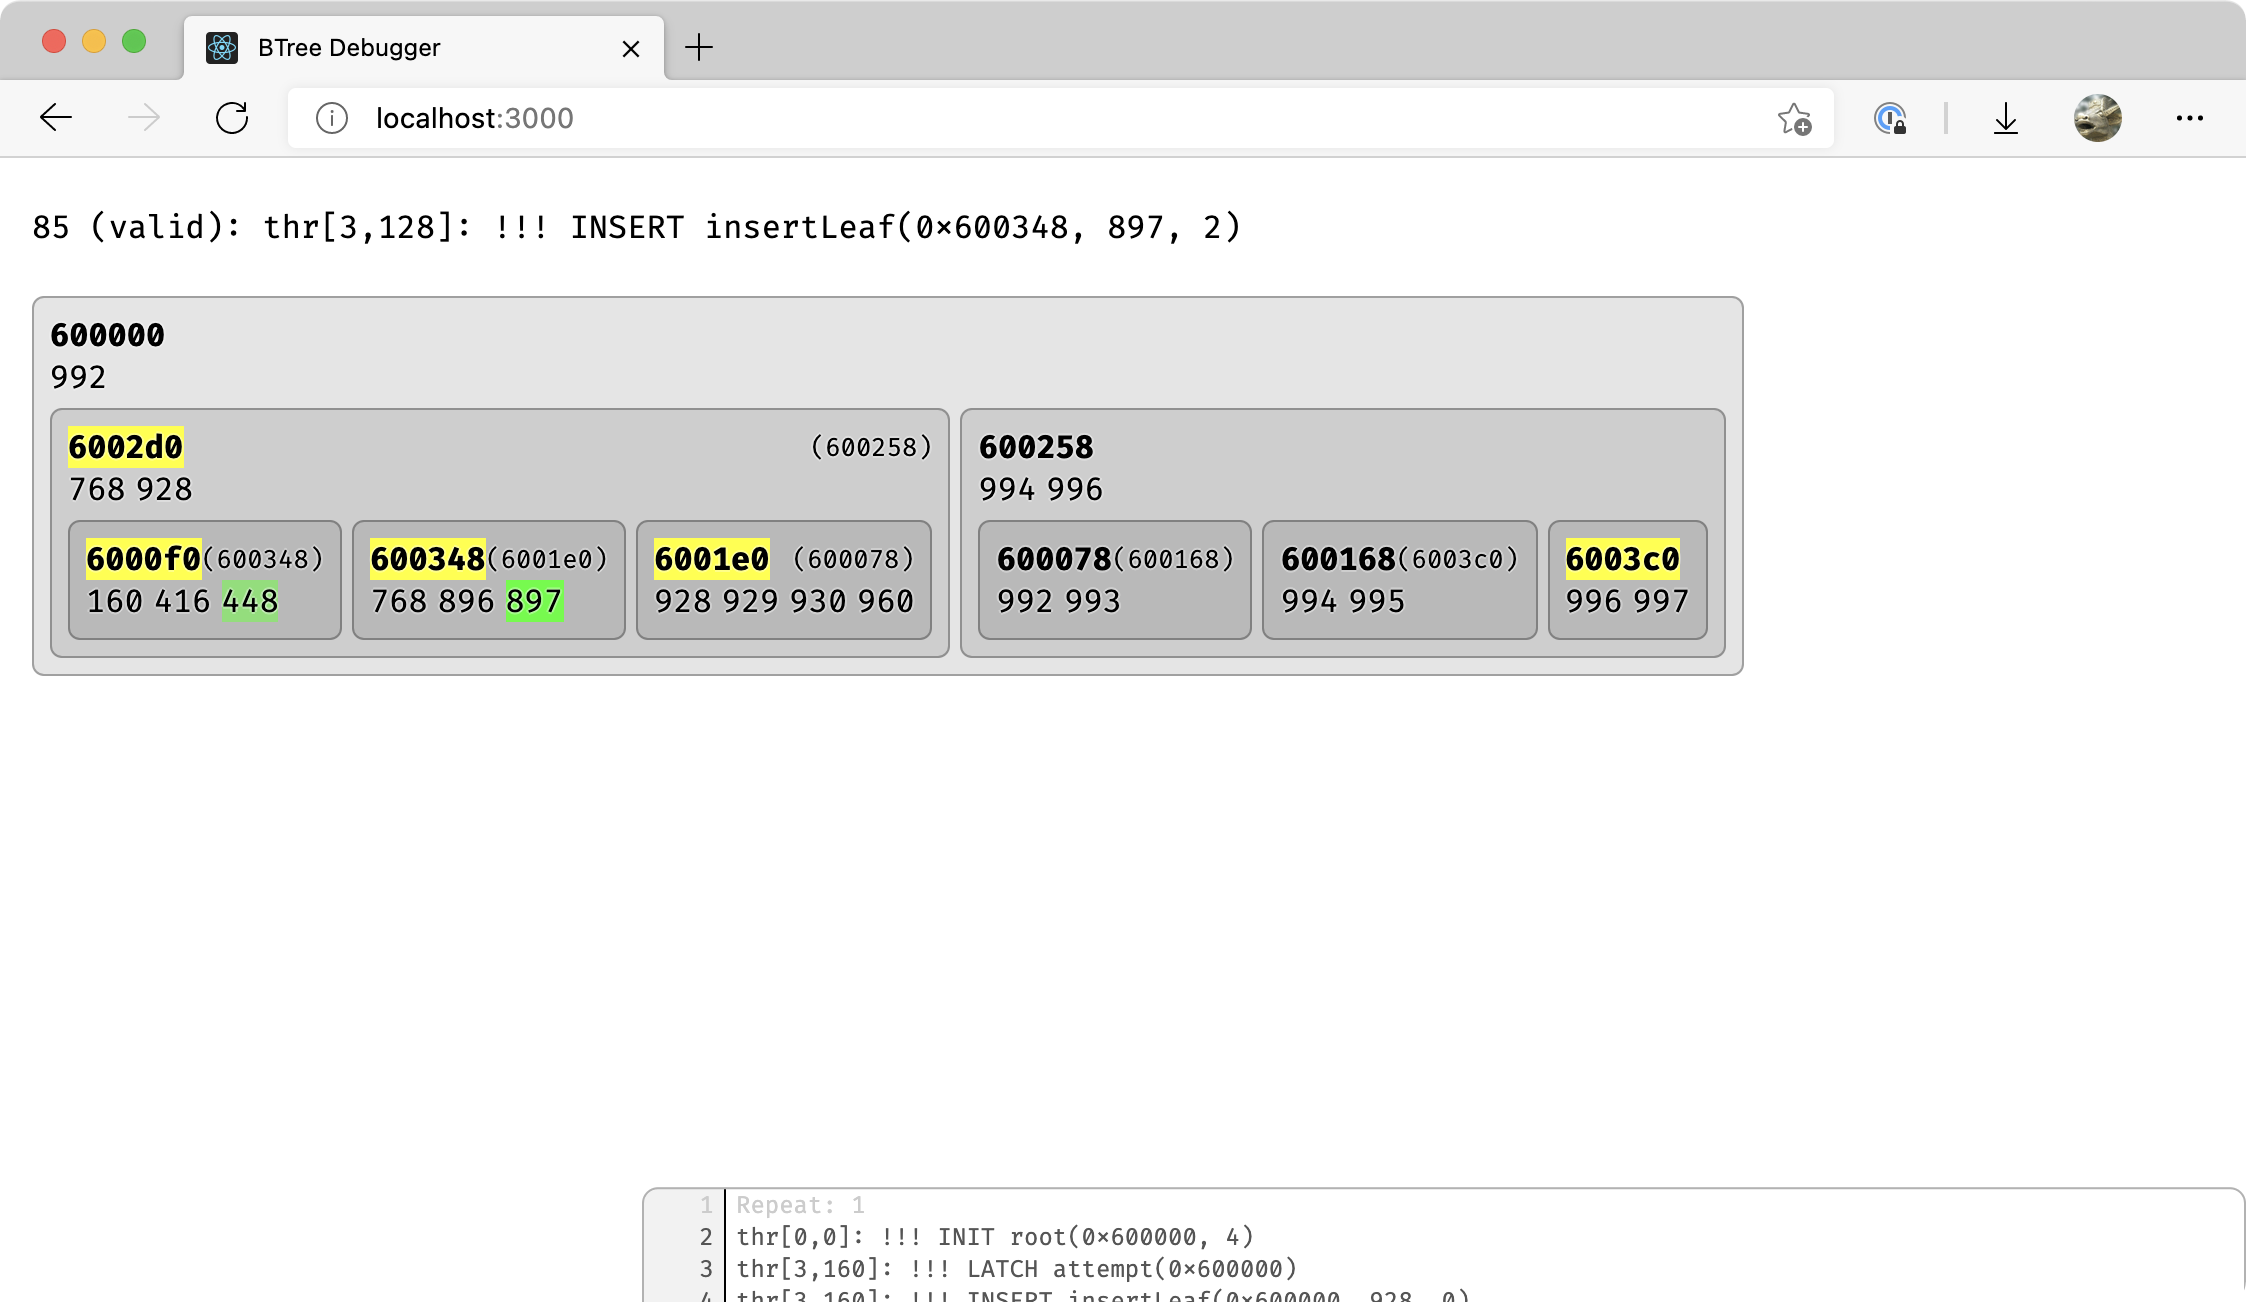
\includegraphics[width=\textwidth]{components/figure/debugger.png}
  \caption{Web based visual debugger displaying the internal state of a tree. Red boxes denote split nodes not yet inserted to the parent node. A highlighted node address indicate that a thread has latched that node.}
  \label{figure:debugger}
\end{figure}

In the case of multiple B-Tree variants, to avoid duplicating tests and ensure the correctness of both implementations, typed tests are used to repeat the same logic over a list of types \cite{gtest-advanced}, as seen in \cref{lst:gtest-typed}. The \code{typename} of each class will be available as a static field within \code{TestFixture} itself.

\begin{listing}
  \begin{minted}{cpp}
template <typename C> class TestSuite : public testing::Test {
public:
  using Implementation = C;
};

using TypeList = ::testing::Types<A, B>;
TYPED_TEST_SUITE(TestSuite, TypeList);

TYPED_TEST(TestSuite, Test) {
  typename TestFixture::Implementation impl;
  // ... rest of test implementation
}
    \end{minted}
  \caption{Snippet of a GoogleTest typed test}\label{lst:gtest-typed}
\end{listing}
\section{Benchmarking methodology}\label{section:benchmarking}

Companion benchmarking methods have been created to provide a standard interface across different implementations of our choice. A tested solution is wrapped in a lambda function, accepting a timer instance and an input sequence as its arguments. This lambda function is invoked ten times, and an arithmetic mean of captured results is computed and stored on a disk. An example code can be seen in \cref{lst:benchmark} and the source code of the benchmarking methods can be found in \code{/benchmark/\_common/benchmark.hpp}.

\begin{listing}
  \begin{minted}{cpp}
using DeviceType = Benchmark::Device::Host;
using NumericType = uint32_t;
Benchmark::execute<DeviceType, NumericType>(
  "test", [](Benchmark::BenchTimer<DeviceType> &timer,
              const std::vector<NumericType> &input) {
    timer.start();
    // insert operation
    timer.stop("insert");

    timer.start();
    // query operation
    timer.stop("query");
  });
  \end{minted}
  \caption{Sample usage of the benchmark methods found in \code{benchmark.hpp}.}
  \label{lst:benchmark}
\end{listing}

The \codecpp{Benchmark::BenchTimer} class will capture the time spent between the invocations of \codecpp{start()} and \codecpp{stop()}. This class does support multiple timers within a single instance by specifying a key string in the stop function, as seen in lines 8 and 12 of \cref{lst:benchmark}. Internally, CPU-based implementations are measured using \codecpp{std::chrono::high_resolution_clock}, whereas GPU-based solutions will use the built-in CUDA runtime API, which is more precise, as it does not include the time spent on potential synchronization.

In most scenarios, the time spent on copying the data between the CPU and GPU were excluded in the actual measurement.

\subsection{Datasets used in benchmarking}\label{subsection:benchmark:datasets}

Different data sequences were generated as the input data for benchmarking created implementations and existing solutions. Assuming $n$ is the expected size of generated data sequence, these datasets were used:

\begin{itemize}
  \item \textit{Ascending} -- sorted sequence $0..(n-1)$,
  \item \textit{Descending} -- inverse of ascending dataset, a sorted sequence $(n-1)..0$,
  \item \textit{Almost sorted} -- sorted sequence $0..(n-1)$ with 5 random swaps,
  \item \textit{Shuffle} -- generated sequence shuffled with \code{std::shuffle},
  \item \textit{Gaussian} -- a sequence generated by producing $n$ random values around mean with standard deviation.
\end{itemize}

For all of the measurements done in \cref{section:results}, 32-bit values are used both as keys and values, as some implementations chosen in \cref{subsection:benchmark:implementations} do not function properly when different data types are utilized. For this reason, no benchmark tests utilizing non-integer keys or values required for comparison on datasets from unstructured numerical meshes are presented here. An example of such a test implemented for TNL based implementations can be found in the source code (\code{/benchmark/tnl/tnl\_mesh\_cuda.cu}).

\subsection{Chosen implementations for comparison}\label{subsection:benchmark:implementations}

As for the implementations themselves, the following projects were chosen for the benchmarks:

\begin{itemize}
  \item \textit{OWG} (owensgroup/GpuBTree) -- implementation of a GPU based B-Link-Tree by Awad et al. \cite{awad},
  \item \textit{PALM} (runshenzhu/palmtree) -- an implementation of PALM Tree \cite{palm} by Xian et al. \cite{palm-impl}; a concurrent lock-free B$^+$Tree scaling up to 16 cores,
  \item \textit{TLX} -- a collection of \CC\,data structures, algorithms and helpers by Bingman et al. \cite{TLX}.
\end{itemize}

\code{std::map} is chosen as the baseline when calculating the performance speedup. Internally, \code{std::map} tends to be implemented as a self-balanced red-black tree \cite{cppreference-map}.

Additional implementations, such as the Bw-Tree implementation by Wang et al. \cite{bwtree-impl}, or STX B$^+$Tree by Timo Bingman \cite{stx-b+tree}, were considered as well. But either due to memory leak issues or deprecation by the author, these solutions were not included in the comparison. Nevertheless, the obtained results can be found in the attached medium.

As the OWG implementation is the only readily available GPU implementation of the B-Tree, additional work has been done to resolve issues encountered while benchmarking. Patches were created for the OWG implementation to mitigate memory leaks. These patches can be found in the benchmarking source code and will be automatically applied when CMake is invoked.

\section{Results}\label{section:results}

Chosen implementations described in \cref{subsection:benchmark:implementations} were measured against different sequences mentioned in \cref{subsection:benchmark:datasets}.

For the speedup comparison, \code{std::map} is chosen as a baseline. 32-bit key-value pairs sequences are generated as the input data. First column indicate the size of the sequence used. Second column contains the raw execution time spent by \code{std::map} on a benchmark test. Remaining speedup values are presented as the ratio of the execution time spent by \code{std::map} to the execution time spent by a tested implementation:

$$\mathit{Speedup} = S = \frac{\tau_{\mathit{CPU}}}{\tau_{\mathit{GPU}}}$$

\subsection{Query performance}
\begin{table}
  \centering
  \begin{tabular}{lr|rrrrrr}
  \toprule
  {}    & STL        & TNL$^+$ & TNL$^{link}$ & OWG      & PALM   & TLX   & TNL$^{host}$ \\
  $2^x$ & $\tau[ms]$ & $S$     & $S$          & $S$      & $S$    & $S$   & $S$          \\
  \midrule
  10    & 0.055      & 0.730   & 0.814        & 1.383    & 1.767  & 0.804 & 0.588        \\
  11    & 0.133      & 1.416   & 1.583        & 2.722    & 1.512  & 0.861 & 0.615        \\
  12    & 0.288      & 3.024   & 3.383        & 5.825    & 2.035  & 0.798 & 0.615        \\
  13    & 0.742      & 7.703   & 8.363        & 14.415   & 3.904  & 0.964 & 0.737        \\
  14    & 1.901      & 11.457  & 16.556       & 30.823   & 4.980  & 1.111 & 0.785        \\
  15    & 4.632      & 21.204  & 21.189       & 36.124   & 5.800  & 1.162 & 0.891        \\
  16    & 10.918     & 29.534  & 25.694       & 44.915   & 7.080  & 1.200 & 0.955        \\
  17    & 26.074     & 32.771  & 33.447       & 61.745   & 8.694  & 1.260 & 0.999        \\
  18    & 62.571     & 34.897  & 38.197       & 78.075   & 10.333 & 1.337 & 0.978        \\
  19    & 169.116    & 49.068  & 51.854       & 105.834  & 13.923 & 1.505 & 1.113        \\
  20    & 480.989    & 121.280 & 74.452       & 153.818  & 19.921 & 1.562 & 1.083        \\
  21    & 1217.690   & 108.249 & 91.548       & 192.396  & 25.343 & 1.617 & 1.269        \\
  22    & 2989.450   & 97.953  & 112.298      & 230.330  & 31.187 & 1.709 & 1.475        \\
  23    & 6975.730   & 187.227 & 138.958      & $\times$ & 36.500 & 1.702 & 1.476        \\
  24    & 16584.300  & 155.728 & 160.673      & $\times$ & 40.687 & 1.789 & 1.476        \\
  25    & 43311.200  & 226.363 & 201.184      & $\times$ & 53.206 & 2.089 & 2.129        \\
  \bottomrule
\end{tabular}


  \caption[Search speed-up compared to \code{std::map}, shuffled sequence.]{Search speed-up of chosen implementations compared to \code{std::map} for various input sizes. \textit{Shuffled} sequence is used as input.}
  \label{table:query-shuffle}
\end{table}

In \cref{table:query-shuffle} the query speedup on \textit{shuffled} sequence is shown. For smaller sequences, \code{std::map} tends to be faster than other compared implementations. However, as the input size increases, the solutions utilizing parallelization overtake the baseline implementation.

As soon as the input size is larger than $2^{10}$, both the TNL$^+$ and TNL$^{link}$ becomes faster than the baseline \code{std::map}. A notable observation can be made when comparing TNL$^+$ (implementation of B$^+$Tree) with TNL$^{link}$ (implementation of B-Link-Tree). Even though the concurrency control is better in TNL$^{link}$ than in TNL$^+$, the reduced instruction count and reduced pointer chasing through sibling links overshadow the performance benefits of such concurrency control, resulting in similar speedup on \textit{shuffled} and \textit{gaussian} input sequence.

\begin{table}
  \centering
  
\begin{tabular}{lr|rrrrrr}
  \toprule
  {}    & STL        & TNL$^+$ & TNL$^{link}$ & OWG      & PALM  & TLX   & TNL$^{host}$ \\
  $2^x$ & $\tau[ms]$ & $S$     & $S$          & $S$      & $S$   & $S$   & $S$          \\
  \midrule
  10    & 0.045      & 0.582   & 0.668        & 1.075    & 1.827 & 0.839 & 0.678        \\
  11    & 0.097      & 1.029   & 1.134        & 1.906    & 1.178 & 0.885 & 0.705        \\
  12    & 0.199      & 2.068   & 2.324        & 4.048    & 1.574 & 0.793 & 0.728        \\
  13    & 0.406      & 3.787   & 4.588        & 7.920    & 2.049 & 0.784 & 0.712        \\
  14    & 0.842      & 4.201   & 6.787        & 13.267   & 2.158 & 0.803 & 0.751        \\
  15    & 1.879      & 7.654   & 10.023       & 14.823   & 2.531 & 0.883 & 0.836        \\
  16    & 4.321      & 9.529   & 10.164       & 17.443   & 2.856 & 0.957 & 0.890        \\
  17    & 10.829     & 10.986  & 11.581       & 23.388   & 3.556 & 1.130 & 1.080        \\
  18    & 26.453     & 15.397  & 15.930       & 30.847   & 4.378 & 1.324 & 1.269        \\
  19    & 60.116     & 17.887  & 18.116       & 35.975   & 4.915 & 1.415 & 1.448        \\
  20    & 128.294    & 15.199  & 17.847       & 35.448   & 5.349 & 1.504 & 1.509        \\
  21    & 271.900    & 18.845  & 19.115       & 38.846   & 5.673 & 1.529 & 1.511        \\
  22    & 602.152    & 23.065  & 20.274       & 43.738   & 6.318 & 1.669 & 1.522        \\
  23    & 1308.570   & 21.677  & 20.167       & $\times$ & 6.905 & 1.739 & 1.797        \\
  24    & 2921.260   & 23.215  & 23.499       & $\times$ & 7.346 & 1.874 & 2.144        \\
  25    & 6591.670   & 25.359  & 26.415       & $\times$ & 8.272 & 2.102 & 2.336        \\
  \bottomrule
\end{tabular}


  \caption[Search speed-up compared to \code{std::map}, ascending sequence.]{Search speed-up of chosen implementations compared to \code{std::map} for various input sizes. \textit{Ascending} sequence is used as input.}
  \label{table:query-increasing}
\end{table}

\begin{figure}
  %% Creator: Matplotlib, PGF backend
%%
%% To include the figure in your LaTeX document, write
%%   \input{<filename>.pgf}
%%
%% Make sure the required packages are loaded in your preamble
%%   \usepackage{pgf}
%%
%% Figures using additional raster images can only be included by \input if
%% they are in the same directory as the main LaTeX file. For loading figures
%% from other directories you can use the `import` package
%%   \usepackage{import}
%%
%% and then include the figures with
%%   \import{<path to file>}{<filename>.pgf}
%%
%% Matplotlib used the following preamble
%%   \usepackage{fontspec}
%%
\begingroup%
\makeatletter%
\begin{pgfpicture}%
\pgfpathrectangle{\pgfpointorigin}{\pgfqpoint{5.065834in}{3.349556in}}%
\pgfusepath{use as bounding box, clip}%
\begin{pgfscope}%
\pgfsetbuttcap%
\pgfsetmiterjoin%
\pgfsetlinewidth{0.000000pt}%
\definecolor{currentstroke}{rgb}{1.000000,1.000000,1.000000}%
\pgfsetstrokecolor{currentstroke}%
\pgfsetstrokeopacity{0.000000}%
\pgfsetdash{}{0pt}%
\pgfpathmoveto{\pgfqpoint{0.000000in}{-0.000000in}}%
\pgfpathlineto{\pgfqpoint{5.065834in}{-0.000000in}}%
\pgfpathlineto{\pgfqpoint{5.065834in}{3.349556in}}%
\pgfpathlineto{\pgfqpoint{0.000000in}{3.349556in}}%
\pgfpathclose%
\pgfusepath{}%
\end{pgfscope}%
\begin{pgfscope}%
\pgfsetbuttcap%
\pgfsetmiterjoin%
\definecolor{currentfill}{rgb}{1.000000,1.000000,1.000000}%
\pgfsetfillcolor{currentfill}%
\pgfsetlinewidth{0.000000pt}%
\definecolor{currentstroke}{rgb}{0.000000,0.000000,0.000000}%
\pgfsetstrokecolor{currentstroke}%
\pgfsetstrokeopacity{0.000000}%
\pgfsetdash{}{0pt}%
\pgfpathmoveto{\pgfqpoint{0.668913in}{1.060056in}}%
\pgfpathlineto{\pgfqpoint{4.626730in}{1.060056in}}%
\pgfpathlineto{\pgfqpoint{4.626730in}{3.249556in}}%
\pgfpathlineto{\pgfqpoint{0.668913in}{3.249556in}}%
\pgfpathclose%
\pgfusepath{fill}%
\end{pgfscope}%
\begin{pgfscope}%
\pgfpathrectangle{\pgfqpoint{0.668913in}{1.060056in}}{\pgfqpoint{3.957816in}{2.189500in}}%
\pgfusepath{clip}%
\pgfsetbuttcap%
\pgfsetroundjoin%
\pgfsetlinewidth{0.702625pt}%
\definecolor{currentstroke}{rgb}{0.827451,0.827451,0.827451}%
\pgfsetstrokecolor{currentstroke}%
\pgfsetdash{{4.480000pt}{1.120000pt}{0.700000pt}{1.120000pt}}{0.000000pt}%
\pgfpathmoveto{\pgfqpoint{1.088681in}{1.060056in}}%
\pgfpathlineto{\pgfqpoint{1.088681in}{3.249556in}}%
\pgfusepath{stroke}%
\end{pgfscope}%
\begin{pgfscope}%
\pgfsetbuttcap%
\pgfsetroundjoin%
\definecolor{currentfill}{rgb}{0.000000,0.000000,0.000000}%
\pgfsetfillcolor{currentfill}%
\pgfsetlinewidth{0.803000pt}%
\definecolor{currentstroke}{rgb}{0.000000,0.000000,0.000000}%
\pgfsetstrokecolor{currentstroke}%
\pgfsetdash{}{0pt}%
\pgfsys@defobject{currentmarker}{\pgfqpoint{0.000000in}{-0.048611in}}{\pgfqpoint{0.000000in}{0.000000in}}{%
\pgfpathmoveto{\pgfqpoint{0.000000in}{0.000000in}}%
\pgfpathlineto{\pgfqpoint{0.000000in}{-0.048611in}}%
\pgfusepath{stroke,fill}%
}%
\begin{pgfscope}%
\pgfsys@transformshift{1.088681in}{1.060056in}%
\pgfsys@useobject{currentmarker}{}%
\end{pgfscope}%
\end{pgfscope}%
\begin{pgfscope}%
\definecolor{textcolor}{rgb}{0.000000,0.000000,0.000000}%
\pgfsetstrokecolor{textcolor}%
\pgfsetfillcolor{textcolor}%
\pgftext[x=1.088681in,y=0.962833in,,top]{\color{textcolor}\rmfamily\fontsize{10.000000}{12.000000}\selectfont \(\displaystyle {2^{11}}\)}%
\end{pgfscope}%
\begin{pgfscope}%
\pgfpathrectangle{\pgfqpoint{0.668913in}{1.060056in}}{\pgfqpoint{3.957816in}{2.189500in}}%
\pgfusepath{clip}%
\pgfsetbuttcap%
\pgfsetroundjoin%
\pgfsetlinewidth{0.702625pt}%
\definecolor{currentstroke}{rgb}{0.827451,0.827451,0.827451}%
\pgfsetstrokecolor{currentstroke}%
\pgfsetdash{{4.480000pt}{1.120000pt}{0.700000pt}{1.120000pt}}{0.000000pt}%
\pgfpathmoveto{\pgfqpoint{1.568417in}{1.060056in}}%
\pgfpathlineto{\pgfqpoint{1.568417in}{3.249556in}}%
\pgfusepath{stroke}%
\end{pgfscope}%
\begin{pgfscope}%
\pgfsetbuttcap%
\pgfsetroundjoin%
\definecolor{currentfill}{rgb}{0.000000,0.000000,0.000000}%
\pgfsetfillcolor{currentfill}%
\pgfsetlinewidth{0.803000pt}%
\definecolor{currentstroke}{rgb}{0.000000,0.000000,0.000000}%
\pgfsetstrokecolor{currentstroke}%
\pgfsetdash{}{0pt}%
\pgfsys@defobject{currentmarker}{\pgfqpoint{0.000000in}{-0.048611in}}{\pgfqpoint{0.000000in}{0.000000in}}{%
\pgfpathmoveto{\pgfqpoint{0.000000in}{0.000000in}}%
\pgfpathlineto{\pgfqpoint{0.000000in}{-0.048611in}}%
\pgfusepath{stroke,fill}%
}%
\begin{pgfscope}%
\pgfsys@transformshift{1.568417in}{1.060056in}%
\pgfsys@useobject{currentmarker}{}%
\end{pgfscope}%
\end{pgfscope}%
\begin{pgfscope}%
\definecolor{textcolor}{rgb}{0.000000,0.000000,0.000000}%
\pgfsetstrokecolor{textcolor}%
\pgfsetfillcolor{textcolor}%
\pgftext[x=1.568417in,y=0.962833in,,top]{\color{textcolor}\rmfamily\fontsize{10.000000}{12.000000}\selectfont \(\displaystyle {2^{13}}\)}%
\end{pgfscope}%
\begin{pgfscope}%
\pgfpathrectangle{\pgfqpoint{0.668913in}{1.060056in}}{\pgfqpoint{3.957816in}{2.189500in}}%
\pgfusepath{clip}%
\pgfsetbuttcap%
\pgfsetroundjoin%
\pgfsetlinewidth{0.702625pt}%
\definecolor{currentstroke}{rgb}{0.827451,0.827451,0.827451}%
\pgfsetstrokecolor{currentstroke}%
\pgfsetdash{{4.480000pt}{1.120000pt}{0.700000pt}{1.120000pt}}{0.000000pt}%
\pgfpathmoveto{\pgfqpoint{2.048152in}{1.060056in}}%
\pgfpathlineto{\pgfqpoint{2.048152in}{3.249556in}}%
\pgfusepath{stroke}%
\end{pgfscope}%
\begin{pgfscope}%
\pgfsetbuttcap%
\pgfsetroundjoin%
\definecolor{currentfill}{rgb}{0.000000,0.000000,0.000000}%
\pgfsetfillcolor{currentfill}%
\pgfsetlinewidth{0.803000pt}%
\definecolor{currentstroke}{rgb}{0.000000,0.000000,0.000000}%
\pgfsetstrokecolor{currentstroke}%
\pgfsetdash{}{0pt}%
\pgfsys@defobject{currentmarker}{\pgfqpoint{0.000000in}{-0.048611in}}{\pgfqpoint{0.000000in}{0.000000in}}{%
\pgfpathmoveto{\pgfqpoint{0.000000in}{0.000000in}}%
\pgfpathlineto{\pgfqpoint{0.000000in}{-0.048611in}}%
\pgfusepath{stroke,fill}%
}%
\begin{pgfscope}%
\pgfsys@transformshift{2.048152in}{1.060056in}%
\pgfsys@useobject{currentmarker}{}%
\end{pgfscope}%
\end{pgfscope}%
\begin{pgfscope}%
\definecolor{textcolor}{rgb}{0.000000,0.000000,0.000000}%
\pgfsetstrokecolor{textcolor}%
\pgfsetfillcolor{textcolor}%
\pgftext[x=2.048152in,y=0.962833in,,top]{\color{textcolor}\rmfamily\fontsize{10.000000}{12.000000}\selectfont \(\displaystyle {2^{15}}\)}%
\end{pgfscope}%
\begin{pgfscope}%
\pgfpathrectangle{\pgfqpoint{0.668913in}{1.060056in}}{\pgfqpoint{3.957816in}{2.189500in}}%
\pgfusepath{clip}%
\pgfsetbuttcap%
\pgfsetroundjoin%
\pgfsetlinewidth{0.702625pt}%
\definecolor{currentstroke}{rgb}{0.827451,0.827451,0.827451}%
\pgfsetstrokecolor{currentstroke}%
\pgfsetdash{{4.480000pt}{1.120000pt}{0.700000pt}{1.120000pt}}{0.000000pt}%
\pgfpathmoveto{\pgfqpoint{2.527887in}{1.060056in}}%
\pgfpathlineto{\pgfqpoint{2.527887in}{3.249556in}}%
\pgfusepath{stroke}%
\end{pgfscope}%
\begin{pgfscope}%
\pgfsetbuttcap%
\pgfsetroundjoin%
\definecolor{currentfill}{rgb}{0.000000,0.000000,0.000000}%
\pgfsetfillcolor{currentfill}%
\pgfsetlinewidth{0.803000pt}%
\definecolor{currentstroke}{rgb}{0.000000,0.000000,0.000000}%
\pgfsetstrokecolor{currentstroke}%
\pgfsetdash{}{0pt}%
\pgfsys@defobject{currentmarker}{\pgfqpoint{0.000000in}{-0.048611in}}{\pgfqpoint{0.000000in}{0.000000in}}{%
\pgfpathmoveto{\pgfqpoint{0.000000in}{0.000000in}}%
\pgfpathlineto{\pgfqpoint{0.000000in}{-0.048611in}}%
\pgfusepath{stroke,fill}%
}%
\begin{pgfscope}%
\pgfsys@transformshift{2.527887in}{1.060056in}%
\pgfsys@useobject{currentmarker}{}%
\end{pgfscope}%
\end{pgfscope}%
\begin{pgfscope}%
\definecolor{textcolor}{rgb}{0.000000,0.000000,0.000000}%
\pgfsetstrokecolor{textcolor}%
\pgfsetfillcolor{textcolor}%
\pgftext[x=2.527887in,y=0.962833in,,top]{\color{textcolor}\rmfamily\fontsize{10.000000}{12.000000}\selectfont \(\displaystyle {2^{17}}\)}%
\end{pgfscope}%
\begin{pgfscope}%
\pgfpathrectangle{\pgfqpoint{0.668913in}{1.060056in}}{\pgfqpoint{3.957816in}{2.189500in}}%
\pgfusepath{clip}%
\pgfsetbuttcap%
\pgfsetroundjoin%
\pgfsetlinewidth{0.702625pt}%
\definecolor{currentstroke}{rgb}{0.827451,0.827451,0.827451}%
\pgfsetstrokecolor{currentstroke}%
\pgfsetdash{{4.480000pt}{1.120000pt}{0.700000pt}{1.120000pt}}{0.000000pt}%
\pgfpathmoveto{\pgfqpoint{3.007623in}{1.060056in}}%
\pgfpathlineto{\pgfqpoint{3.007623in}{3.249556in}}%
\pgfusepath{stroke}%
\end{pgfscope}%
\begin{pgfscope}%
\pgfsetbuttcap%
\pgfsetroundjoin%
\definecolor{currentfill}{rgb}{0.000000,0.000000,0.000000}%
\pgfsetfillcolor{currentfill}%
\pgfsetlinewidth{0.803000pt}%
\definecolor{currentstroke}{rgb}{0.000000,0.000000,0.000000}%
\pgfsetstrokecolor{currentstroke}%
\pgfsetdash{}{0pt}%
\pgfsys@defobject{currentmarker}{\pgfqpoint{0.000000in}{-0.048611in}}{\pgfqpoint{0.000000in}{0.000000in}}{%
\pgfpathmoveto{\pgfqpoint{0.000000in}{0.000000in}}%
\pgfpathlineto{\pgfqpoint{0.000000in}{-0.048611in}}%
\pgfusepath{stroke,fill}%
}%
\begin{pgfscope}%
\pgfsys@transformshift{3.007623in}{1.060056in}%
\pgfsys@useobject{currentmarker}{}%
\end{pgfscope}%
\end{pgfscope}%
\begin{pgfscope}%
\definecolor{textcolor}{rgb}{0.000000,0.000000,0.000000}%
\pgfsetstrokecolor{textcolor}%
\pgfsetfillcolor{textcolor}%
\pgftext[x=3.007623in,y=0.962833in,,top]{\color{textcolor}\rmfamily\fontsize{10.000000}{12.000000}\selectfont \(\displaystyle {2^{19}}\)}%
\end{pgfscope}%
\begin{pgfscope}%
\pgfpathrectangle{\pgfqpoint{0.668913in}{1.060056in}}{\pgfqpoint{3.957816in}{2.189500in}}%
\pgfusepath{clip}%
\pgfsetbuttcap%
\pgfsetroundjoin%
\pgfsetlinewidth{0.702625pt}%
\definecolor{currentstroke}{rgb}{0.827451,0.827451,0.827451}%
\pgfsetstrokecolor{currentstroke}%
\pgfsetdash{{4.480000pt}{1.120000pt}{0.700000pt}{1.120000pt}}{0.000000pt}%
\pgfpathmoveto{\pgfqpoint{3.487358in}{1.060056in}}%
\pgfpathlineto{\pgfqpoint{3.487358in}{3.249556in}}%
\pgfusepath{stroke}%
\end{pgfscope}%
\begin{pgfscope}%
\pgfsetbuttcap%
\pgfsetroundjoin%
\definecolor{currentfill}{rgb}{0.000000,0.000000,0.000000}%
\pgfsetfillcolor{currentfill}%
\pgfsetlinewidth{0.803000pt}%
\definecolor{currentstroke}{rgb}{0.000000,0.000000,0.000000}%
\pgfsetstrokecolor{currentstroke}%
\pgfsetdash{}{0pt}%
\pgfsys@defobject{currentmarker}{\pgfqpoint{0.000000in}{-0.048611in}}{\pgfqpoint{0.000000in}{0.000000in}}{%
\pgfpathmoveto{\pgfqpoint{0.000000in}{0.000000in}}%
\pgfpathlineto{\pgfqpoint{0.000000in}{-0.048611in}}%
\pgfusepath{stroke,fill}%
}%
\begin{pgfscope}%
\pgfsys@transformshift{3.487358in}{1.060056in}%
\pgfsys@useobject{currentmarker}{}%
\end{pgfscope}%
\end{pgfscope}%
\begin{pgfscope}%
\definecolor{textcolor}{rgb}{0.000000,0.000000,0.000000}%
\pgfsetstrokecolor{textcolor}%
\pgfsetfillcolor{textcolor}%
\pgftext[x=3.487358in,y=0.962833in,,top]{\color{textcolor}\rmfamily\fontsize{10.000000}{12.000000}\selectfont \(\displaystyle {2^{21}}\)}%
\end{pgfscope}%
\begin{pgfscope}%
\pgfpathrectangle{\pgfqpoint{0.668913in}{1.060056in}}{\pgfqpoint{3.957816in}{2.189500in}}%
\pgfusepath{clip}%
\pgfsetbuttcap%
\pgfsetroundjoin%
\pgfsetlinewidth{0.702625pt}%
\definecolor{currentstroke}{rgb}{0.827451,0.827451,0.827451}%
\pgfsetstrokecolor{currentstroke}%
\pgfsetdash{{4.480000pt}{1.120000pt}{0.700000pt}{1.120000pt}}{0.000000pt}%
\pgfpathmoveto{\pgfqpoint{3.967093in}{1.060056in}}%
\pgfpathlineto{\pgfqpoint{3.967093in}{3.249556in}}%
\pgfusepath{stroke}%
\end{pgfscope}%
\begin{pgfscope}%
\pgfsetbuttcap%
\pgfsetroundjoin%
\definecolor{currentfill}{rgb}{0.000000,0.000000,0.000000}%
\pgfsetfillcolor{currentfill}%
\pgfsetlinewidth{0.803000pt}%
\definecolor{currentstroke}{rgb}{0.000000,0.000000,0.000000}%
\pgfsetstrokecolor{currentstroke}%
\pgfsetdash{}{0pt}%
\pgfsys@defobject{currentmarker}{\pgfqpoint{0.000000in}{-0.048611in}}{\pgfqpoint{0.000000in}{0.000000in}}{%
\pgfpathmoveto{\pgfqpoint{0.000000in}{0.000000in}}%
\pgfpathlineto{\pgfqpoint{0.000000in}{-0.048611in}}%
\pgfusepath{stroke,fill}%
}%
\begin{pgfscope}%
\pgfsys@transformshift{3.967093in}{1.060056in}%
\pgfsys@useobject{currentmarker}{}%
\end{pgfscope}%
\end{pgfscope}%
\begin{pgfscope}%
\definecolor{textcolor}{rgb}{0.000000,0.000000,0.000000}%
\pgfsetstrokecolor{textcolor}%
\pgfsetfillcolor{textcolor}%
\pgftext[x=3.967093in,y=0.962833in,,top]{\color{textcolor}\rmfamily\fontsize{10.000000}{12.000000}\selectfont \(\displaystyle {2^{23}}\)}%
\end{pgfscope}%
\begin{pgfscope}%
\pgfpathrectangle{\pgfqpoint{0.668913in}{1.060056in}}{\pgfqpoint{3.957816in}{2.189500in}}%
\pgfusepath{clip}%
\pgfsetbuttcap%
\pgfsetroundjoin%
\pgfsetlinewidth{0.702625pt}%
\definecolor{currentstroke}{rgb}{0.827451,0.827451,0.827451}%
\pgfsetstrokecolor{currentstroke}%
\pgfsetdash{{4.480000pt}{1.120000pt}{0.700000pt}{1.120000pt}}{0.000000pt}%
\pgfpathmoveto{\pgfqpoint{4.446829in}{1.060056in}}%
\pgfpathlineto{\pgfqpoint{4.446829in}{3.249556in}}%
\pgfusepath{stroke}%
\end{pgfscope}%
\begin{pgfscope}%
\pgfsetbuttcap%
\pgfsetroundjoin%
\definecolor{currentfill}{rgb}{0.000000,0.000000,0.000000}%
\pgfsetfillcolor{currentfill}%
\pgfsetlinewidth{0.803000pt}%
\definecolor{currentstroke}{rgb}{0.000000,0.000000,0.000000}%
\pgfsetstrokecolor{currentstroke}%
\pgfsetdash{}{0pt}%
\pgfsys@defobject{currentmarker}{\pgfqpoint{0.000000in}{-0.048611in}}{\pgfqpoint{0.000000in}{0.000000in}}{%
\pgfpathmoveto{\pgfqpoint{0.000000in}{0.000000in}}%
\pgfpathlineto{\pgfqpoint{0.000000in}{-0.048611in}}%
\pgfusepath{stroke,fill}%
}%
\begin{pgfscope}%
\pgfsys@transformshift{4.446829in}{1.060056in}%
\pgfsys@useobject{currentmarker}{}%
\end{pgfscope}%
\end{pgfscope}%
\begin{pgfscope}%
\definecolor{textcolor}{rgb}{0.000000,0.000000,0.000000}%
\pgfsetstrokecolor{textcolor}%
\pgfsetfillcolor{textcolor}%
\pgftext[x=4.446829in,y=0.962833in,,top]{\color{textcolor}\rmfamily\fontsize{10.000000}{12.000000}\selectfont \(\displaystyle {2^{25}}\)}%
\end{pgfscope}%
\begin{pgfscope}%
\definecolor{textcolor}{rgb}{0.000000,0.000000,0.000000}%
\pgfsetstrokecolor{textcolor}%
\pgfsetfillcolor{textcolor}%
\pgftext[x=2.647821in,y=0.783945in,,top]{\color{textcolor}\rmfamily\fontsize{10.000000}{12.000000}\selectfont Number of items}%
\end{pgfscope}%
\begin{pgfscope}%
\pgfpathrectangle{\pgfqpoint{0.668913in}{1.060056in}}{\pgfqpoint{3.957816in}{2.189500in}}%
\pgfusepath{clip}%
\pgfsetbuttcap%
\pgfsetroundjoin%
\pgfsetlinewidth{0.702625pt}%
\definecolor{currentstroke}{rgb}{0.827451,0.827451,0.827451}%
\pgfsetstrokecolor{currentstroke}%
\pgfsetdash{{4.480000pt}{1.120000pt}{0.700000pt}{1.120000pt}}{0.000000pt}%
\pgfpathmoveto{\pgfqpoint{0.668913in}{1.218652in}}%
\pgfpathlineto{\pgfqpoint{4.626730in}{1.218652in}}%
\pgfusepath{stroke}%
\end{pgfscope}%
\begin{pgfscope}%
\pgfsetbuttcap%
\pgfsetroundjoin%
\definecolor{currentfill}{rgb}{0.000000,0.000000,0.000000}%
\pgfsetfillcolor{currentfill}%
\pgfsetlinewidth{0.803000pt}%
\definecolor{currentstroke}{rgb}{0.000000,0.000000,0.000000}%
\pgfsetstrokecolor{currentstroke}%
\pgfsetdash{}{0pt}%
\pgfsys@defobject{currentmarker}{\pgfqpoint{-0.048611in}{0.000000in}}{\pgfqpoint{-0.000000in}{0.000000in}}{%
\pgfpathmoveto{\pgfqpoint{-0.000000in}{0.000000in}}%
\pgfpathlineto{\pgfqpoint{-0.048611in}{0.000000in}}%
\pgfusepath{stroke,fill}%
}%
\begin{pgfscope}%
\pgfsys@transformshift{0.668913in}{1.218652in}%
\pgfsys@useobject{currentmarker}{}%
\end{pgfscope}%
\end{pgfscope}%
\begin{pgfscope}%
\definecolor{textcolor}{rgb}{0.000000,0.000000,0.000000}%
\pgfsetstrokecolor{textcolor}%
\pgfsetfillcolor{textcolor}%
\pgftext[x=0.370494in, y=1.170458in, left, base]{\color{textcolor}\rmfamily\fontsize{10.000000}{12.000000}\selectfont \(\displaystyle {10^{6}}\)}%
\end{pgfscope}%
\begin{pgfscope}%
\pgfpathrectangle{\pgfqpoint{0.668913in}{1.060056in}}{\pgfqpoint{3.957816in}{2.189500in}}%
\pgfusepath{clip}%
\pgfsetbuttcap%
\pgfsetroundjoin%
\pgfsetlinewidth{0.702625pt}%
\definecolor{currentstroke}{rgb}{0.827451,0.827451,0.827451}%
\pgfsetstrokecolor{currentstroke}%
\pgfsetdash{{4.480000pt}{1.120000pt}{0.700000pt}{1.120000pt}}{0.000000pt}%
\pgfpathmoveto{\pgfqpoint{0.668913in}{1.982901in}}%
\pgfpathlineto{\pgfqpoint{4.626730in}{1.982901in}}%
\pgfusepath{stroke}%
\end{pgfscope}%
\begin{pgfscope}%
\pgfsetbuttcap%
\pgfsetroundjoin%
\definecolor{currentfill}{rgb}{0.000000,0.000000,0.000000}%
\pgfsetfillcolor{currentfill}%
\pgfsetlinewidth{0.803000pt}%
\definecolor{currentstroke}{rgb}{0.000000,0.000000,0.000000}%
\pgfsetstrokecolor{currentstroke}%
\pgfsetdash{}{0pt}%
\pgfsys@defobject{currentmarker}{\pgfqpoint{-0.048611in}{0.000000in}}{\pgfqpoint{-0.000000in}{0.000000in}}{%
\pgfpathmoveto{\pgfqpoint{-0.000000in}{0.000000in}}%
\pgfpathlineto{\pgfqpoint{-0.048611in}{0.000000in}}%
\pgfusepath{stroke,fill}%
}%
\begin{pgfscope}%
\pgfsys@transformshift{0.668913in}{1.982901in}%
\pgfsys@useobject{currentmarker}{}%
\end{pgfscope}%
\end{pgfscope}%
\begin{pgfscope}%
\definecolor{textcolor}{rgb}{0.000000,0.000000,0.000000}%
\pgfsetstrokecolor{textcolor}%
\pgfsetfillcolor{textcolor}%
\pgftext[x=0.370494in, y=1.934706in, left, base]{\color{textcolor}\rmfamily\fontsize{10.000000}{12.000000}\selectfont \(\displaystyle {10^{7}}\)}%
\end{pgfscope}%
\begin{pgfscope}%
\pgfpathrectangle{\pgfqpoint{0.668913in}{1.060056in}}{\pgfqpoint{3.957816in}{2.189500in}}%
\pgfusepath{clip}%
\pgfsetbuttcap%
\pgfsetroundjoin%
\pgfsetlinewidth{0.702625pt}%
\definecolor{currentstroke}{rgb}{0.827451,0.827451,0.827451}%
\pgfsetstrokecolor{currentstroke}%
\pgfsetdash{{4.480000pt}{1.120000pt}{0.700000pt}{1.120000pt}}{0.000000pt}%
\pgfpathmoveto{\pgfqpoint{0.668913in}{2.747149in}}%
\pgfpathlineto{\pgfqpoint{4.626730in}{2.747149in}}%
\pgfusepath{stroke}%
\end{pgfscope}%
\begin{pgfscope}%
\pgfsetbuttcap%
\pgfsetroundjoin%
\definecolor{currentfill}{rgb}{0.000000,0.000000,0.000000}%
\pgfsetfillcolor{currentfill}%
\pgfsetlinewidth{0.803000pt}%
\definecolor{currentstroke}{rgb}{0.000000,0.000000,0.000000}%
\pgfsetstrokecolor{currentstroke}%
\pgfsetdash{}{0pt}%
\pgfsys@defobject{currentmarker}{\pgfqpoint{-0.048611in}{0.000000in}}{\pgfqpoint{-0.000000in}{0.000000in}}{%
\pgfpathmoveto{\pgfqpoint{-0.000000in}{0.000000in}}%
\pgfpathlineto{\pgfqpoint{-0.048611in}{0.000000in}}%
\pgfusepath{stroke,fill}%
}%
\begin{pgfscope}%
\pgfsys@transformshift{0.668913in}{2.747149in}%
\pgfsys@useobject{currentmarker}{}%
\end{pgfscope}%
\end{pgfscope}%
\begin{pgfscope}%
\definecolor{textcolor}{rgb}{0.000000,0.000000,0.000000}%
\pgfsetstrokecolor{textcolor}%
\pgfsetfillcolor{textcolor}%
\pgftext[x=0.370494in, y=2.698955in, left, base]{\color{textcolor}\rmfamily\fontsize{10.000000}{12.000000}\selectfont \(\displaystyle {10^{8}}\)}%
\end{pgfscope}%
\begin{pgfscope}%
\pgfsetbuttcap%
\pgfsetroundjoin%
\definecolor{currentfill}{rgb}{0.000000,0.000000,0.000000}%
\pgfsetfillcolor{currentfill}%
\pgfsetlinewidth{0.602250pt}%
\definecolor{currentstroke}{rgb}{0.000000,0.000000,0.000000}%
\pgfsetstrokecolor{currentstroke}%
\pgfsetdash{}{0pt}%
\pgfsys@defobject{currentmarker}{\pgfqpoint{-0.027778in}{0.000000in}}{\pgfqpoint{-0.000000in}{0.000000in}}{%
\pgfpathmoveto{\pgfqpoint{-0.000000in}{0.000000in}}%
\pgfpathlineto{\pgfqpoint{-0.027778in}{0.000000in}}%
\pgfusepath{stroke,fill}%
}%
\begin{pgfscope}%
\pgfsys@transformshift{0.668913in}{1.100269in}%
\pgfsys@useobject{currentmarker}{}%
\end{pgfscope}%
\end{pgfscope}%
\begin{pgfscope}%
\pgfsetbuttcap%
\pgfsetroundjoin%
\definecolor{currentfill}{rgb}{0.000000,0.000000,0.000000}%
\pgfsetfillcolor{currentfill}%
\pgfsetlinewidth{0.602250pt}%
\definecolor{currentstroke}{rgb}{0.000000,0.000000,0.000000}%
\pgfsetstrokecolor{currentstroke}%
\pgfsetdash{}{0pt}%
\pgfsys@defobject{currentmarker}{\pgfqpoint{-0.027778in}{0.000000in}}{\pgfqpoint{-0.000000in}{0.000000in}}{%
\pgfpathmoveto{\pgfqpoint{-0.000000in}{0.000000in}}%
\pgfpathlineto{\pgfqpoint{-0.027778in}{0.000000in}}%
\pgfusepath{stroke,fill}%
}%
\begin{pgfscope}%
\pgfsys@transformshift{0.668913in}{1.144589in}%
\pgfsys@useobject{currentmarker}{}%
\end{pgfscope}%
\end{pgfscope}%
\begin{pgfscope}%
\pgfsetbuttcap%
\pgfsetroundjoin%
\definecolor{currentfill}{rgb}{0.000000,0.000000,0.000000}%
\pgfsetfillcolor{currentfill}%
\pgfsetlinewidth{0.602250pt}%
\definecolor{currentstroke}{rgb}{0.000000,0.000000,0.000000}%
\pgfsetstrokecolor{currentstroke}%
\pgfsetdash{}{0pt}%
\pgfsys@defobject{currentmarker}{\pgfqpoint{-0.027778in}{0.000000in}}{\pgfqpoint{-0.000000in}{0.000000in}}{%
\pgfpathmoveto{\pgfqpoint{-0.000000in}{0.000000in}}%
\pgfpathlineto{\pgfqpoint{-0.027778in}{0.000000in}}%
\pgfusepath{stroke,fill}%
}%
\begin{pgfscope}%
\pgfsys@transformshift{0.668913in}{1.183682in}%
\pgfsys@useobject{currentmarker}{}%
\end{pgfscope}%
\end{pgfscope}%
\begin{pgfscope}%
\pgfsetbuttcap%
\pgfsetroundjoin%
\definecolor{currentfill}{rgb}{0.000000,0.000000,0.000000}%
\pgfsetfillcolor{currentfill}%
\pgfsetlinewidth{0.602250pt}%
\definecolor{currentstroke}{rgb}{0.000000,0.000000,0.000000}%
\pgfsetstrokecolor{currentstroke}%
\pgfsetdash{}{0pt}%
\pgfsys@defobject{currentmarker}{\pgfqpoint{-0.027778in}{0.000000in}}{\pgfqpoint{-0.000000in}{0.000000in}}{%
\pgfpathmoveto{\pgfqpoint{-0.000000in}{0.000000in}}%
\pgfpathlineto{\pgfqpoint{-0.027778in}{0.000000in}}%
\pgfusepath{stroke,fill}%
}%
\begin{pgfscope}%
\pgfsys@transformshift{0.668913in}{1.448714in}%
\pgfsys@useobject{currentmarker}{}%
\end{pgfscope}%
\end{pgfscope}%
\begin{pgfscope}%
\pgfsetbuttcap%
\pgfsetroundjoin%
\definecolor{currentfill}{rgb}{0.000000,0.000000,0.000000}%
\pgfsetfillcolor{currentfill}%
\pgfsetlinewidth{0.602250pt}%
\definecolor{currentstroke}{rgb}{0.000000,0.000000,0.000000}%
\pgfsetstrokecolor{currentstroke}%
\pgfsetdash{}{0pt}%
\pgfsys@defobject{currentmarker}{\pgfqpoint{-0.027778in}{0.000000in}}{\pgfqpoint{-0.000000in}{0.000000in}}{%
\pgfpathmoveto{\pgfqpoint{-0.000000in}{0.000000in}}%
\pgfpathlineto{\pgfqpoint{-0.027778in}{0.000000in}}%
\pgfusepath{stroke,fill}%
}%
\begin{pgfscope}%
\pgfsys@transformshift{0.668913in}{1.583292in}%
\pgfsys@useobject{currentmarker}{}%
\end{pgfscope}%
\end{pgfscope}%
\begin{pgfscope}%
\pgfsetbuttcap%
\pgfsetroundjoin%
\definecolor{currentfill}{rgb}{0.000000,0.000000,0.000000}%
\pgfsetfillcolor{currentfill}%
\pgfsetlinewidth{0.602250pt}%
\definecolor{currentstroke}{rgb}{0.000000,0.000000,0.000000}%
\pgfsetstrokecolor{currentstroke}%
\pgfsetdash{}{0pt}%
\pgfsys@defobject{currentmarker}{\pgfqpoint{-0.027778in}{0.000000in}}{\pgfqpoint{-0.000000in}{0.000000in}}{%
\pgfpathmoveto{\pgfqpoint{-0.000000in}{0.000000in}}%
\pgfpathlineto{\pgfqpoint{-0.027778in}{0.000000in}}%
\pgfusepath{stroke,fill}%
}%
\begin{pgfscope}%
\pgfsys@transformshift{0.668913in}{1.678776in}%
\pgfsys@useobject{currentmarker}{}%
\end{pgfscope}%
\end{pgfscope}%
\begin{pgfscope}%
\pgfsetbuttcap%
\pgfsetroundjoin%
\definecolor{currentfill}{rgb}{0.000000,0.000000,0.000000}%
\pgfsetfillcolor{currentfill}%
\pgfsetlinewidth{0.602250pt}%
\definecolor{currentstroke}{rgb}{0.000000,0.000000,0.000000}%
\pgfsetstrokecolor{currentstroke}%
\pgfsetdash{}{0pt}%
\pgfsys@defobject{currentmarker}{\pgfqpoint{-0.027778in}{0.000000in}}{\pgfqpoint{-0.000000in}{0.000000in}}{%
\pgfpathmoveto{\pgfqpoint{-0.000000in}{0.000000in}}%
\pgfpathlineto{\pgfqpoint{-0.027778in}{0.000000in}}%
\pgfusepath{stroke,fill}%
}%
\begin{pgfscope}%
\pgfsys@transformshift{0.668913in}{1.752839in}%
\pgfsys@useobject{currentmarker}{}%
\end{pgfscope}%
\end{pgfscope}%
\begin{pgfscope}%
\pgfsetbuttcap%
\pgfsetroundjoin%
\definecolor{currentfill}{rgb}{0.000000,0.000000,0.000000}%
\pgfsetfillcolor{currentfill}%
\pgfsetlinewidth{0.602250pt}%
\definecolor{currentstroke}{rgb}{0.000000,0.000000,0.000000}%
\pgfsetstrokecolor{currentstroke}%
\pgfsetdash{}{0pt}%
\pgfsys@defobject{currentmarker}{\pgfqpoint{-0.027778in}{0.000000in}}{\pgfqpoint{-0.000000in}{0.000000in}}{%
\pgfpathmoveto{\pgfqpoint{-0.000000in}{0.000000in}}%
\pgfpathlineto{\pgfqpoint{-0.027778in}{0.000000in}}%
\pgfusepath{stroke,fill}%
}%
\begin{pgfscope}%
\pgfsys@transformshift{0.668913in}{1.813353in}%
\pgfsys@useobject{currentmarker}{}%
\end{pgfscope}%
\end{pgfscope}%
\begin{pgfscope}%
\pgfsetbuttcap%
\pgfsetroundjoin%
\definecolor{currentfill}{rgb}{0.000000,0.000000,0.000000}%
\pgfsetfillcolor{currentfill}%
\pgfsetlinewidth{0.602250pt}%
\definecolor{currentstroke}{rgb}{0.000000,0.000000,0.000000}%
\pgfsetstrokecolor{currentstroke}%
\pgfsetdash{}{0pt}%
\pgfsys@defobject{currentmarker}{\pgfqpoint{-0.027778in}{0.000000in}}{\pgfqpoint{-0.000000in}{0.000000in}}{%
\pgfpathmoveto{\pgfqpoint{-0.000000in}{0.000000in}}%
\pgfpathlineto{\pgfqpoint{-0.027778in}{0.000000in}}%
\pgfusepath{stroke,fill}%
}%
\begin{pgfscope}%
\pgfsys@transformshift{0.668913in}{1.864517in}%
\pgfsys@useobject{currentmarker}{}%
\end{pgfscope}%
\end{pgfscope}%
\begin{pgfscope}%
\pgfsetbuttcap%
\pgfsetroundjoin%
\definecolor{currentfill}{rgb}{0.000000,0.000000,0.000000}%
\pgfsetfillcolor{currentfill}%
\pgfsetlinewidth{0.602250pt}%
\definecolor{currentstroke}{rgb}{0.000000,0.000000,0.000000}%
\pgfsetstrokecolor{currentstroke}%
\pgfsetdash{}{0pt}%
\pgfsys@defobject{currentmarker}{\pgfqpoint{-0.027778in}{0.000000in}}{\pgfqpoint{-0.000000in}{0.000000in}}{%
\pgfpathmoveto{\pgfqpoint{-0.000000in}{0.000000in}}%
\pgfpathlineto{\pgfqpoint{-0.027778in}{0.000000in}}%
\pgfusepath{stroke,fill}%
}%
\begin{pgfscope}%
\pgfsys@transformshift{0.668913in}{1.908838in}%
\pgfsys@useobject{currentmarker}{}%
\end{pgfscope}%
\end{pgfscope}%
\begin{pgfscope}%
\pgfsetbuttcap%
\pgfsetroundjoin%
\definecolor{currentfill}{rgb}{0.000000,0.000000,0.000000}%
\pgfsetfillcolor{currentfill}%
\pgfsetlinewidth{0.602250pt}%
\definecolor{currentstroke}{rgb}{0.000000,0.000000,0.000000}%
\pgfsetstrokecolor{currentstroke}%
\pgfsetdash{}{0pt}%
\pgfsys@defobject{currentmarker}{\pgfqpoint{-0.027778in}{0.000000in}}{\pgfqpoint{-0.000000in}{0.000000in}}{%
\pgfpathmoveto{\pgfqpoint{-0.000000in}{0.000000in}}%
\pgfpathlineto{\pgfqpoint{-0.027778in}{0.000000in}}%
\pgfusepath{stroke,fill}%
}%
\begin{pgfscope}%
\pgfsys@transformshift{0.668913in}{1.947931in}%
\pgfsys@useobject{currentmarker}{}%
\end{pgfscope}%
\end{pgfscope}%
\begin{pgfscope}%
\pgfsetbuttcap%
\pgfsetroundjoin%
\definecolor{currentfill}{rgb}{0.000000,0.000000,0.000000}%
\pgfsetfillcolor{currentfill}%
\pgfsetlinewidth{0.602250pt}%
\definecolor{currentstroke}{rgb}{0.000000,0.000000,0.000000}%
\pgfsetstrokecolor{currentstroke}%
\pgfsetdash{}{0pt}%
\pgfsys@defobject{currentmarker}{\pgfqpoint{-0.027778in}{0.000000in}}{\pgfqpoint{-0.000000in}{0.000000in}}{%
\pgfpathmoveto{\pgfqpoint{-0.000000in}{0.000000in}}%
\pgfpathlineto{\pgfqpoint{-0.027778in}{0.000000in}}%
\pgfusepath{stroke,fill}%
}%
\begin{pgfscope}%
\pgfsys@transformshift{0.668913in}{2.212963in}%
\pgfsys@useobject{currentmarker}{}%
\end{pgfscope}%
\end{pgfscope}%
\begin{pgfscope}%
\pgfsetbuttcap%
\pgfsetroundjoin%
\definecolor{currentfill}{rgb}{0.000000,0.000000,0.000000}%
\pgfsetfillcolor{currentfill}%
\pgfsetlinewidth{0.602250pt}%
\definecolor{currentstroke}{rgb}{0.000000,0.000000,0.000000}%
\pgfsetstrokecolor{currentstroke}%
\pgfsetdash{}{0pt}%
\pgfsys@defobject{currentmarker}{\pgfqpoint{-0.027778in}{0.000000in}}{\pgfqpoint{-0.000000in}{0.000000in}}{%
\pgfpathmoveto{\pgfqpoint{-0.000000in}{0.000000in}}%
\pgfpathlineto{\pgfqpoint{-0.027778in}{0.000000in}}%
\pgfusepath{stroke,fill}%
}%
\begin{pgfscope}%
\pgfsys@transformshift{0.668913in}{2.347540in}%
\pgfsys@useobject{currentmarker}{}%
\end{pgfscope}%
\end{pgfscope}%
\begin{pgfscope}%
\pgfsetbuttcap%
\pgfsetroundjoin%
\definecolor{currentfill}{rgb}{0.000000,0.000000,0.000000}%
\pgfsetfillcolor{currentfill}%
\pgfsetlinewidth{0.602250pt}%
\definecolor{currentstroke}{rgb}{0.000000,0.000000,0.000000}%
\pgfsetstrokecolor{currentstroke}%
\pgfsetdash{}{0pt}%
\pgfsys@defobject{currentmarker}{\pgfqpoint{-0.027778in}{0.000000in}}{\pgfqpoint{-0.000000in}{0.000000in}}{%
\pgfpathmoveto{\pgfqpoint{-0.000000in}{0.000000in}}%
\pgfpathlineto{\pgfqpoint{-0.027778in}{0.000000in}}%
\pgfusepath{stroke,fill}%
}%
\begin{pgfscope}%
\pgfsys@transformshift{0.668913in}{2.443024in}%
\pgfsys@useobject{currentmarker}{}%
\end{pgfscope}%
\end{pgfscope}%
\begin{pgfscope}%
\pgfsetbuttcap%
\pgfsetroundjoin%
\definecolor{currentfill}{rgb}{0.000000,0.000000,0.000000}%
\pgfsetfillcolor{currentfill}%
\pgfsetlinewidth{0.602250pt}%
\definecolor{currentstroke}{rgb}{0.000000,0.000000,0.000000}%
\pgfsetstrokecolor{currentstroke}%
\pgfsetdash{}{0pt}%
\pgfsys@defobject{currentmarker}{\pgfqpoint{-0.027778in}{0.000000in}}{\pgfqpoint{-0.000000in}{0.000000in}}{%
\pgfpathmoveto{\pgfqpoint{-0.000000in}{0.000000in}}%
\pgfpathlineto{\pgfqpoint{-0.027778in}{0.000000in}}%
\pgfusepath{stroke,fill}%
}%
\begin{pgfscope}%
\pgfsys@transformshift{0.668913in}{2.517088in}%
\pgfsys@useobject{currentmarker}{}%
\end{pgfscope}%
\end{pgfscope}%
\begin{pgfscope}%
\pgfsetbuttcap%
\pgfsetroundjoin%
\definecolor{currentfill}{rgb}{0.000000,0.000000,0.000000}%
\pgfsetfillcolor{currentfill}%
\pgfsetlinewidth{0.602250pt}%
\definecolor{currentstroke}{rgb}{0.000000,0.000000,0.000000}%
\pgfsetstrokecolor{currentstroke}%
\pgfsetdash{}{0pt}%
\pgfsys@defobject{currentmarker}{\pgfqpoint{-0.027778in}{0.000000in}}{\pgfqpoint{-0.000000in}{0.000000in}}{%
\pgfpathmoveto{\pgfqpoint{-0.000000in}{0.000000in}}%
\pgfpathlineto{\pgfqpoint{-0.027778in}{0.000000in}}%
\pgfusepath{stroke,fill}%
}%
\begin{pgfscope}%
\pgfsys@transformshift{0.668913in}{2.577602in}%
\pgfsys@useobject{currentmarker}{}%
\end{pgfscope}%
\end{pgfscope}%
\begin{pgfscope}%
\pgfsetbuttcap%
\pgfsetroundjoin%
\definecolor{currentfill}{rgb}{0.000000,0.000000,0.000000}%
\pgfsetfillcolor{currentfill}%
\pgfsetlinewidth{0.602250pt}%
\definecolor{currentstroke}{rgb}{0.000000,0.000000,0.000000}%
\pgfsetstrokecolor{currentstroke}%
\pgfsetdash{}{0pt}%
\pgfsys@defobject{currentmarker}{\pgfqpoint{-0.027778in}{0.000000in}}{\pgfqpoint{-0.000000in}{0.000000in}}{%
\pgfpathmoveto{\pgfqpoint{-0.000000in}{0.000000in}}%
\pgfpathlineto{\pgfqpoint{-0.027778in}{0.000000in}}%
\pgfusepath{stroke,fill}%
}%
\begin{pgfscope}%
\pgfsys@transformshift{0.668913in}{2.628766in}%
\pgfsys@useobject{currentmarker}{}%
\end{pgfscope}%
\end{pgfscope}%
\begin{pgfscope}%
\pgfsetbuttcap%
\pgfsetroundjoin%
\definecolor{currentfill}{rgb}{0.000000,0.000000,0.000000}%
\pgfsetfillcolor{currentfill}%
\pgfsetlinewidth{0.602250pt}%
\definecolor{currentstroke}{rgb}{0.000000,0.000000,0.000000}%
\pgfsetstrokecolor{currentstroke}%
\pgfsetdash{}{0pt}%
\pgfsys@defobject{currentmarker}{\pgfqpoint{-0.027778in}{0.000000in}}{\pgfqpoint{-0.000000in}{0.000000in}}{%
\pgfpathmoveto{\pgfqpoint{-0.000000in}{0.000000in}}%
\pgfpathlineto{\pgfqpoint{-0.027778in}{0.000000in}}%
\pgfusepath{stroke,fill}%
}%
\begin{pgfscope}%
\pgfsys@transformshift{0.668913in}{2.673086in}%
\pgfsys@useobject{currentmarker}{}%
\end{pgfscope}%
\end{pgfscope}%
\begin{pgfscope}%
\pgfsetbuttcap%
\pgfsetroundjoin%
\definecolor{currentfill}{rgb}{0.000000,0.000000,0.000000}%
\pgfsetfillcolor{currentfill}%
\pgfsetlinewidth{0.602250pt}%
\definecolor{currentstroke}{rgb}{0.000000,0.000000,0.000000}%
\pgfsetstrokecolor{currentstroke}%
\pgfsetdash{}{0pt}%
\pgfsys@defobject{currentmarker}{\pgfqpoint{-0.027778in}{0.000000in}}{\pgfqpoint{-0.000000in}{0.000000in}}{%
\pgfpathmoveto{\pgfqpoint{-0.000000in}{0.000000in}}%
\pgfpathlineto{\pgfqpoint{-0.027778in}{0.000000in}}%
\pgfusepath{stroke,fill}%
}%
\begin{pgfscope}%
\pgfsys@transformshift{0.668913in}{2.712179in}%
\pgfsys@useobject{currentmarker}{}%
\end{pgfscope}%
\end{pgfscope}%
\begin{pgfscope}%
\pgfsetbuttcap%
\pgfsetroundjoin%
\definecolor{currentfill}{rgb}{0.000000,0.000000,0.000000}%
\pgfsetfillcolor{currentfill}%
\pgfsetlinewidth{0.602250pt}%
\definecolor{currentstroke}{rgb}{0.000000,0.000000,0.000000}%
\pgfsetstrokecolor{currentstroke}%
\pgfsetdash{}{0pt}%
\pgfsys@defobject{currentmarker}{\pgfqpoint{-0.027778in}{0.000000in}}{\pgfqpoint{-0.000000in}{0.000000in}}{%
\pgfpathmoveto{\pgfqpoint{-0.000000in}{0.000000in}}%
\pgfpathlineto{\pgfqpoint{-0.027778in}{0.000000in}}%
\pgfusepath{stroke,fill}%
}%
\begin{pgfscope}%
\pgfsys@transformshift{0.668913in}{2.977211in}%
\pgfsys@useobject{currentmarker}{}%
\end{pgfscope}%
\end{pgfscope}%
\begin{pgfscope}%
\pgfsetbuttcap%
\pgfsetroundjoin%
\definecolor{currentfill}{rgb}{0.000000,0.000000,0.000000}%
\pgfsetfillcolor{currentfill}%
\pgfsetlinewidth{0.602250pt}%
\definecolor{currentstroke}{rgb}{0.000000,0.000000,0.000000}%
\pgfsetstrokecolor{currentstroke}%
\pgfsetdash{}{0pt}%
\pgfsys@defobject{currentmarker}{\pgfqpoint{-0.027778in}{0.000000in}}{\pgfqpoint{-0.000000in}{0.000000in}}{%
\pgfpathmoveto{\pgfqpoint{-0.000000in}{0.000000in}}%
\pgfpathlineto{\pgfqpoint{-0.027778in}{0.000000in}}%
\pgfusepath{stroke,fill}%
}%
\begin{pgfscope}%
\pgfsys@transformshift{0.668913in}{3.111789in}%
\pgfsys@useobject{currentmarker}{}%
\end{pgfscope}%
\end{pgfscope}%
\begin{pgfscope}%
\pgfsetbuttcap%
\pgfsetroundjoin%
\definecolor{currentfill}{rgb}{0.000000,0.000000,0.000000}%
\pgfsetfillcolor{currentfill}%
\pgfsetlinewidth{0.602250pt}%
\definecolor{currentstroke}{rgb}{0.000000,0.000000,0.000000}%
\pgfsetstrokecolor{currentstroke}%
\pgfsetdash{}{0pt}%
\pgfsys@defobject{currentmarker}{\pgfqpoint{-0.027778in}{0.000000in}}{\pgfqpoint{-0.000000in}{0.000000in}}{%
\pgfpathmoveto{\pgfqpoint{-0.000000in}{0.000000in}}%
\pgfpathlineto{\pgfqpoint{-0.027778in}{0.000000in}}%
\pgfusepath{stroke,fill}%
}%
\begin{pgfscope}%
\pgfsys@transformshift{0.668913in}{3.207273in}%
\pgfsys@useobject{currentmarker}{}%
\end{pgfscope}%
\end{pgfscope}%
\begin{pgfscope}%
\definecolor{textcolor}{rgb}{0.000000,0.000000,0.000000}%
\pgfsetstrokecolor{textcolor}%
\pgfsetfillcolor{textcolor}%
\pgftext[x=0.314939in,y=2.154806in,,bottom,rotate=90.000000]{\color{textcolor}\rmfamily\fontsize{10.000000}{12.000000}\selectfont Operations per second}%
\end{pgfscope}%
\begin{pgfscope}%
\pgfpathrectangle{\pgfqpoint{0.668913in}{1.060056in}}{\pgfqpoint{3.957816in}{2.189500in}}%
\pgfusepath{clip}%
\pgfsetrectcap%
\pgfsetroundjoin%
\pgfsetlinewidth{1.505625pt}%
\definecolor{currentstroke}{rgb}{0.121569,0.466667,0.705882}%
\pgfsetstrokecolor{currentstroke}%
\pgfsetdash{}{0pt}%
\pgfpathmoveto{\pgfqpoint{0.848814in}{2.200244in}}%
\pgfpathlineto{\pgfqpoint{1.088681in}{2.161151in}}%
\pgfpathlineto{\pgfqpoint{1.328549in}{2.115137in}}%
\pgfpathlineto{\pgfqpoint{1.568417in}{2.045105in}}%
\pgfpathlineto{\pgfqpoint{1.808284in}{1.956097in}}%
\pgfpathlineto{\pgfqpoint{2.048152in}{1.883585in}}%
\pgfpathlineto{\pgfqpoint{2.288020in}{1.826089in}}%
\pgfpathlineto{\pgfqpoint{2.527887in}{1.772079in}}%
\pgfpathlineto{\pgfqpoint{2.767755in}{1.708224in}}%
\pgfpathlineto{\pgfqpoint{3.007623in}{1.632793in}}%
\pgfpathlineto{\pgfqpoint{3.247490in}{1.516307in}}%
\pgfpathlineto{\pgfqpoint{3.487358in}{1.401290in}}%
\pgfpathlineto{\pgfqpoint{3.727226in}{1.336926in}}%
\pgfpathlineto{\pgfqpoint{3.967093in}{1.286618in}}%
\pgfpathlineto{\pgfqpoint{4.206961in}{1.209789in}}%
\pgfpathlineto{\pgfqpoint{4.446829in}{1.159578in}}%
\pgfusepath{stroke}%
\end{pgfscope}%
\begin{pgfscope}%
\pgfpathrectangle{\pgfqpoint{0.668913in}{1.060056in}}{\pgfqpoint{3.957816in}{2.189500in}}%
\pgfusepath{clip}%
\pgfsetbuttcap%
\pgfsetroundjoin%
\definecolor{currentfill}{rgb}{0.121569,0.466667,0.705882}%
\pgfsetfillcolor{currentfill}%
\pgfsetlinewidth{1.003750pt}%
\definecolor{currentstroke}{rgb}{0.121569,0.466667,0.705882}%
\pgfsetstrokecolor{currentstroke}%
\pgfsetdash{}{0pt}%
\pgfsys@defobject{currentmarker}{\pgfqpoint{-0.020833in}{-0.020833in}}{\pgfqpoint{0.020833in}{0.020833in}}{%
\pgfpathmoveto{\pgfqpoint{0.000000in}{-0.020833in}}%
\pgfpathcurveto{\pgfqpoint{0.005525in}{-0.020833in}}{\pgfqpoint{0.010825in}{-0.018638in}}{\pgfqpoint{0.014731in}{-0.014731in}}%
\pgfpathcurveto{\pgfqpoint{0.018638in}{-0.010825in}}{\pgfqpoint{0.020833in}{-0.005525in}}{\pgfqpoint{0.020833in}{0.000000in}}%
\pgfpathcurveto{\pgfqpoint{0.020833in}{0.005525in}}{\pgfqpoint{0.018638in}{0.010825in}}{\pgfqpoint{0.014731in}{0.014731in}}%
\pgfpathcurveto{\pgfqpoint{0.010825in}{0.018638in}}{\pgfqpoint{0.005525in}{0.020833in}}{\pgfqpoint{0.000000in}{0.020833in}}%
\pgfpathcurveto{\pgfqpoint{-0.005525in}{0.020833in}}{\pgfqpoint{-0.010825in}{0.018638in}}{\pgfqpoint{-0.014731in}{0.014731in}}%
\pgfpathcurveto{\pgfqpoint{-0.018638in}{0.010825in}}{\pgfqpoint{-0.020833in}{0.005525in}}{\pgfqpoint{-0.020833in}{0.000000in}}%
\pgfpathcurveto{\pgfqpoint{-0.020833in}{-0.005525in}}{\pgfqpoint{-0.018638in}{-0.010825in}}{\pgfqpoint{-0.014731in}{-0.014731in}}%
\pgfpathcurveto{\pgfqpoint{-0.010825in}{-0.018638in}}{\pgfqpoint{-0.005525in}{-0.020833in}}{\pgfqpoint{0.000000in}{-0.020833in}}%
\pgfpathclose%
\pgfusepath{stroke,fill}%
}%
\begin{pgfscope}%
\pgfsys@transformshift{0.848814in}{2.200244in}%
\pgfsys@useobject{currentmarker}{}%
\end{pgfscope}%
\begin{pgfscope}%
\pgfsys@transformshift{1.088681in}{2.161151in}%
\pgfsys@useobject{currentmarker}{}%
\end{pgfscope}%
\begin{pgfscope}%
\pgfsys@transformshift{1.328549in}{2.115137in}%
\pgfsys@useobject{currentmarker}{}%
\end{pgfscope}%
\begin{pgfscope}%
\pgfsys@transformshift{1.568417in}{2.045105in}%
\pgfsys@useobject{currentmarker}{}%
\end{pgfscope}%
\begin{pgfscope}%
\pgfsys@transformshift{1.808284in}{1.956097in}%
\pgfsys@useobject{currentmarker}{}%
\end{pgfscope}%
\begin{pgfscope}%
\pgfsys@transformshift{2.048152in}{1.883585in}%
\pgfsys@useobject{currentmarker}{}%
\end{pgfscope}%
\begin{pgfscope}%
\pgfsys@transformshift{2.288020in}{1.826089in}%
\pgfsys@useobject{currentmarker}{}%
\end{pgfscope}%
\begin{pgfscope}%
\pgfsys@transformshift{2.527887in}{1.772079in}%
\pgfsys@useobject{currentmarker}{}%
\end{pgfscope}%
\begin{pgfscope}%
\pgfsys@transformshift{2.767755in}{1.708224in}%
\pgfsys@useobject{currentmarker}{}%
\end{pgfscope}%
\begin{pgfscope}%
\pgfsys@transformshift{3.007623in}{1.632793in}%
\pgfsys@useobject{currentmarker}{}%
\end{pgfscope}%
\begin{pgfscope}%
\pgfsys@transformshift{3.247490in}{1.516307in}%
\pgfsys@useobject{currentmarker}{}%
\end{pgfscope}%
\begin{pgfscope}%
\pgfsys@transformshift{3.487358in}{1.401290in}%
\pgfsys@useobject{currentmarker}{}%
\end{pgfscope}%
\begin{pgfscope}%
\pgfsys@transformshift{3.727226in}{1.336926in}%
\pgfsys@useobject{currentmarker}{}%
\end{pgfscope}%
\begin{pgfscope}%
\pgfsys@transformshift{3.967093in}{1.286618in}%
\pgfsys@useobject{currentmarker}{}%
\end{pgfscope}%
\begin{pgfscope}%
\pgfsys@transformshift{4.206961in}{1.209789in}%
\pgfsys@useobject{currentmarker}{}%
\end{pgfscope}%
\begin{pgfscope}%
\pgfsys@transformshift{4.446829in}{1.159578in}%
\pgfsys@useobject{currentmarker}{}%
\end{pgfscope}%
\end{pgfscope}%
\begin{pgfscope}%
\pgfpathrectangle{\pgfqpoint{0.668913in}{1.060056in}}{\pgfqpoint{3.957816in}{2.189500in}}%
\pgfusepath{clip}%
\pgfsetrectcap%
\pgfsetroundjoin%
\pgfsetlinewidth{1.505625pt}%
\definecolor{currentstroke}{rgb}{1.000000,0.498039,0.054902}%
\pgfsetstrokecolor{currentstroke}%
\pgfsetdash{}{0pt}%
\pgfpathmoveto{\pgfqpoint{0.848814in}{2.090210in}}%
\pgfpathlineto{\pgfqpoint{1.088681in}{2.243810in}}%
\pgfpathlineto{\pgfqpoint{1.328549in}{2.467223in}}%
\pgfpathlineto{\pgfqpoint{1.568417in}{2.699523in}}%
\pgfpathlineto{\pgfqpoint{1.808284in}{2.808494in}}%
\pgfpathlineto{\pgfqpoint{2.048152in}{2.840094in}}%
\pgfpathlineto{\pgfqpoint{2.288020in}{2.814733in}}%
\pgfpathlineto{\pgfqpoint{2.527887in}{2.905647in}}%
\pgfpathlineto{\pgfqpoint{2.767755in}{3.025134in}}%
\pgfpathlineto{\pgfqpoint{3.007623in}{2.929035in}}%
\pgfpathlineto{\pgfqpoint{3.247490in}{2.915040in}}%
\pgfpathlineto{\pgfqpoint{3.487358in}{2.989563in}}%
\pgfpathlineto{\pgfqpoint{3.727226in}{2.945562in}}%
\pgfpathlineto{\pgfqpoint{3.967093in}{2.868632in}}%
\pgfpathlineto{\pgfqpoint{4.206961in}{2.996685in}}%
\pgfpathlineto{\pgfqpoint{4.446829in}{2.967386in}}%
\pgfusepath{stroke}%
\end{pgfscope}%
\begin{pgfscope}%
\pgfpathrectangle{\pgfqpoint{0.668913in}{1.060056in}}{\pgfqpoint{3.957816in}{2.189500in}}%
\pgfusepath{clip}%
\pgfsetbuttcap%
\pgfsetroundjoin%
\definecolor{currentfill}{rgb}{1.000000,0.498039,0.054902}%
\pgfsetfillcolor{currentfill}%
\pgfsetlinewidth{1.003750pt}%
\definecolor{currentstroke}{rgb}{1.000000,0.498039,0.054902}%
\pgfsetstrokecolor{currentstroke}%
\pgfsetdash{}{0pt}%
\pgfsys@defobject{currentmarker}{\pgfqpoint{-0.020833in}{-0.020833in}}{\pgfqpoint{0.020833in}{0.020833in}}{%
\pgfpathmoveto{\pgfqpoint{0.000000in}{-0.020833in}}%
\pgfpathcurveto{\pgfqpoint{0.005525in}{-0.020833in}}{\pgfqpoint{0.010825in}{-0.018638in}}{\pgfqpoint{0.014731in}{-0.014731in}}%
\pgfpathcurveto{\pgfqpoint{0.018638in}{-0.010825in}}{\pgfqpoint{0.020833in}{-0.005525in}}{\pgfqpoint{0.020833in}{0.000000in}}%
\pgfpathcurveto{\pgfqpoint{0.020833in}{0.005525in}}{\pgfqpoint{0.018638in}{0.010825in}}{\pgfqpoint{0.014731in}{0.014731in}}%
\pgfpathcurveto{\pgfqpoint{0.010825in}{0.018638in}}{\pgfqpoint{0.005525in}{0.020833in}}{\pgfqpoint{0.000000in}{0.020833in}}%
\pgfpathcurveto{\pgfqpoint{-0.005525in}{0.020833in}}{\pgfqpoint{-0.010825in}{0.018638in}}{\pgfqpoint{-0.014731in}{0.014731in}}%
\pgfpathcurveto{\pgfqpoint{-0.018638in}{0.010825in}}{\pgfqpoint{-0.020833in}{0.005525in}}{\pgfqpoint{-0.020833in}{0.000000in}}%
\pgfpathcurveto{\pgfqpoint{-0.020833in}{-0.005525in}}{\pgfqpoint{-0.018638in}{-0.010825in}}{\pgfqpoint{-0.014731in}{-0.014731in}}%
\pgfpathcurveto{\pgfqpoint{-0.010825in}{-0.018638in}}{\pgfqpoint{-0.005525in}{-0.020833in}}{\pgfqpoint{0.000000in}{-0.020833in}}%
\pgfpathclose%
\pgfusepath{stroke,fill}%
}%
\begin{pgfscope}%
\pgfsys@transformshift{0.848814in}{2.090210in}%
\pgfsys@useobject{currentmarker}{}%
\end{pgfscope}%
\begin{pgfscope}%
\pgfsys@transformshift{1.088681in}{2.243810in}%
\pgfsys@useobject{currentmarker}{}%
\end{pgfscope}%
\begin{pgfscope}%
\pgfsys@transformshift{1.328549in}{2.467223in}%
\pgfsys@useobject{currentmarker}{}%
\end{pgfscope}%
\begin{pgfscope}%
\pgfsys@transformshift{1.568417in}{2.699523in}%
\pgfsys@useobject{currentmarker}{}%
\end{pgfscope}%
\begin{pgfscope}%
\pgfsys@transformshift{1.808284in}{2.808494in}%
\pgfsys@useobject{currentmarker}{}%
\end{pgfscope}%
\begin{pgfscope}%
\pgfsys@transformshift{2.048152in}{2.840094in}%
\pgfsys@useobject{currentmarker}{}%
\end{pgfscope}%
\begin{pgfscope}%
\pgfsys@transformshift{2.288020in}{2.814733in}%
\pgfsys@useobject{currentmarker}{}%
\end{pgfscope}%
\begin{pgfscope}%
\pgfsys@transformshift{2.527887in}{2.905647in}%
\pgfsys@useobject{currentmarker}{}%
\end{pgfscope}%
\begin{pgfscope}%
\pgfsys@transformshift{2.767755in}{3.025134in}%
\pgfsys@useobject{currentmarker}{}%
\end{pgfscope}%
\begin{pgfscope}%
\pgfsys@transformshift{3.007623in}{2.929035in}%
\pgfsys@useobject{currentmarker}{}%
\end{pgfscope}%
\begin{pgfscope}%
\pgfsys@transformshift{3.247490in}{2.915040in}%
\pgfsys@useobject{currentmarker}{}%
\end{pgfscope}%
\begin{pgfscope}%
\pgfsys@transformshift{3.487358in}{2.989563in}%
\pgfsys@useobject{currentmarker}{}%
\end{pgfscope}%
\begin{pgfscope}%
\pgfsys@transformshift{3.727226in}{2.945562in}%
\pgfsys@useobject{currentmarker}{}%
\end{pgfscope}%
\begin{pgfscope}%
\pgfsys@transformshift{3.967093in}{2.868632in}%
\pgfsys@useobject{currentmarker}{}%
\end{pgfscope}%
\begin{pgfscope}%
\pgfsys@transformshift{4.206961in}{2.996685in}%
\pgfsys@useobject{currentmarker}{}%
\end{pgfscope}%
\begin{pgfscope}%
\pgfsys@transformshift{4.446829in}{2.967386in}%
\pgfsys@useobject{currentmarker}{}%
\end{pgfscope}%
\end{pgfscope}%
\begin{pgfscope}%
\pgfpathrectangle{\pgfqpoint{0.668913in}{1.060056in}}{\pgfqpoint{3.957816in}{2.189500in}}%
\pgfusepath{clip}%
\pgfsetrectcap%
\pgfsetroundjoin%
\pgfsetlinewidth{1.505625pt}%
\definecolor{currentstroke}{rgb}{0.172549,0.627451,0.172549}%
\pgfsetstrokecolor{currentstroke}%
\pgfsetdash{}{0pt}%
\pgfpathmoveto{\pgfqpoint{0.848814in}{2.121822in}}%
\pgfpathlineto{\pgfqpoint{1.088681in}{2.276009in}}%
\pgfpathlineto{\pgfqpoint{1.328549in}{2.505908in}}%
\pgfpathlineto{\pgfqpoint{1.568417in}{2.728765in}}%
\pgfpathlineto{\pgfqpoint{1.808284in}{2.851897in}}%
\pgfpathlineto{\pgfqpoint{2.048152in}{2.893428in}}%
\pgfpathlineto{\pgfqpoint{2.288020in}{2.881157in}}%
\pgfpathlineto{\pgfqpoint{2.527887in}{2.893839in}}%
\pgfpathlineto{\pgfqpoint{2.767755in}{2.920330in}}%
\pgfpathlineto{\pgfqpoint{3.007623in}{2.936267in}}%
\pgfpathlineto{\pgfqpoint{3.247490in}{2.918483in}}%
\pgfpathlineto{\pgfqpoint{3.487358in}{2.895565in}}%
\pgfpathlineto{\pgfqpoint{3.727226in}{2.933563in}}%
\pgfpathlineto{\pgfqpoint{3.967093in}{2.873115in}}%
\pgfpathlineto{\pgfqpoint{4.206961in}{2.900995in}}%
\pgfpathlineto{\pgfqpoint{4.446829in}{2.938830in}}%
\pgfusepath{stroke}%
\end{pgfscope}%
\begin{pgfscope}%
\pgfpathrectangle{\pgfqpoint{0.668913in}{1.060056in}}{\pgfqpoint{3.957816in}{2.189500in}}%
\pgfusepath{clip}%
\pgfsetbuttcap%
\pgfsetroundjoin%
\definecolor{currentfill}{rgb}{0.172549,0.627451,0.172549}%
\pgfsetfillcolor{currentfill}%
\pgfsetlinewidth{1.003750pt}%
\definecolor{currentstroke}{rgb}{0.172549,0.627451,0.172549}%
\pgfsetstrokecolor{currentstroke}%
\pgfsetdash{}{0pt}%
\pgfsys@defobject{currentmarker}{\pgfqpoint{-0.020833in}{-0.020833in}}{\pgfqpoint{0.020833in}{0.020833in}}{%
\pgfpathmoveto{\pgfqpoint{0.000000in}{-0.020833in}}%
\pgfpathcurveto{\pgfqpoint{0.005525in}{-0.020833in}}{\pgfqpoint{0.010825in}{-0.018638in}}{\pgfqpoint{0.014731in}{-0.014731in}}%
\pgfpathcurveto{\pgfqpoint{0.018638in}{-0.010825in}}{\pgfqpoint{0.020833in}{-0.005525in}}{\pgfqpoint{0.020833in}{0.000000in}}%
\pgfpathcurveto{\pgfqpoint{0.020833in}{0.005525in}}{\pgfqpoint{0.018638in}{0.010825in}}{\pgfqpoint{0.014731in}{0.014731in}}%
\pgfpathcurveto{\pgfqpoint{0.010825in}{0.018638in}}{\pgfqpoint{0.005525in}{0.020833in}}{\pgfqpoint{0.000000in}{0.020833in}}%
\pgfpathcurveto{\pgfqpoint{-0.005525in}{0.020833in}}{\pgfqpoint{-0.010825in}{0.018638in}}{\pgfqpoint{-0.014731in}{0.014731in}}%
\pgfpathcurveto{\pgfqpoint{-0.018638in}{0.010825in}}{\pgfqpoint{-0.020833in}{0.005525in}}{\pgfqpoint{-0.020833in}{0.000000in}}%
\pgfpathcurveto{\pgfqpoint{-0.020833in}{-0.005525in}}{\pgfqpoint{-0.018638in}{-0.010825in}}{\pgfqpoint{-0.014731in}{-0.014731in}}%
\pgfpathcurveto{\pgfqpoint{-0.010825in}{-0.018638in}}{\pgfqpoint{-0.005525in}{-0.020833in}}{\pgfqpoint{0.000000in}{-0.020833in}}%
\pgfpathclose%
\pgfusepath{stroke,fill}%
}%
\begin{pgfscope}%
\pgfsys@transformshift{0.848814in}{2.121822in}%
\pgfsys@useobject{currentmarker}{}%
\end{pgfscope}%
\begin{pgfscope}%
\pgfsys@transformshift{1.088681in}{2.276009in}%
\pgfsys@useobject{currentmarker}{}%
\end{pgfscope}%
\begin{pgfscope}%
\pgfsys@transformshift{1.328549in}{2.505908in}%
\pgfsys@useobject{currentmarker}{}%
\end{pgfscope}%
\begin{pgfscope}%
\pgfsys@transformshift{1.568417in}{2.728765in}%
\pgfsys@useobject{currentmarker}{}%
\end{pgfscope}%
\begin{pgfscope}%
\pgfsys@transformshift{1.808284in}{2.851897in}%
\pgfsys@useobject{currentmarker}{}%
\end{pgfscope}%
\begin{pgfscope}%
\pgfsys@transformshift{2.048152in}{2.893428in}%
\pgfsys@useobject{currentmarker}{}%
\end{pgfscope}%
\begin{pgfscope}%
\pgfsys@transformshift{2.288020in}{2.881157in}%
\pgfsys@useobject{currentmarker}{}%
\end{pgfscope}%
\begin{pgfscope}%
\pgfsys@transformshift{2.527887in}{2.893839in}%
\pgfsys@useobject{currentmarker}{}%
\end{pgfscope}%
\begin{pgfscope}%
\pgfsys@transformshift{2.767755in}{2.920330in}%
\pgfsys@useobject{currentmarker}{}%
\end{pgfscope}%
\begin{pgfscope}%
\pgfsys@transformshift{3.007623in}{2.936267in}%
\pgfsys@useobject{currentmarker}{}%
\end{pgfscope}%
\begin{pgfscope}%
\pgfsys@transformshift{3.247490in}{2.918483in}%
\pgfsys@useobject{currentmarker}{}%
\end{pgfscope}%
\begin{pgfscope}%
\pgfsys@transformshift{3.487358in}{2.895565in}%
\pgfsys@useobject{currentmarker}{}%
\end{pgfscope}%
\begin{pgfscope}%
\pgfsys@transformshift{3.727226in}{2.933563in}%
\pgfsys@useobject{currentmarker}{}%
\end{pgfscope}%
\begin{pgfscope}%
\pgfsys@transformshift{3.967093in}{2.873115in}%
\pgfsys@useobject{currentmarker}{}%
\end{pgfscope}%
\begin{pgfscope}%
\pgfsys@transformshift{4.206961in}{2.900995in}%
\pgfsys@useobject{currentmarker}{}%
\end{pgfscope}%
\begin{pgfscope}%
\pgfsys@transformshift{4.446829in}{2.938830in}%
\pgfsys@useobject{currentmarker}{}%
\end{pgfscope}%
\end{pgfscope}%
\begin{pgfscope}%
\pgfpathrectangle{\pgfqpoint{0.668913in}{1.060056in}}{\pgfqpoint{3.957816in}{2.189500in}}%
\pgfusepath{clip}%
\pgfsetrectcap%
\pgfsetroundjoin%
\pgfsetlinewidth{1.505625pt}%
\definecolor{currentstroke}{rgb}{0.839216,0.152941,0.156863}%
\pgfsetstrokecolor{currentstroke}%
\pgfsetdash{}{0pt}%
\pgfpathmoveto{\pgfqpoint{0.848814in}{2.296628in}}%
\pgfpathlineto{\pgfqpoint{1.088681in}{2.457461in}}%
\pgfpathlineto{\pgfqpoint{1.328549in}{2.686851in}}%
\pgfpathlineto{\pgfqpoint{1.568417in}{2.904561in}}%
\pgfpathlineto{\pgfqpoint{1.808284in}{3.112619in}}%
\pgfpathlineto{\pgfqpoint{2.048152in}{3.050142in}}%
\pgfpathlineto{\pgfqpoint{2.288020in}{3.073193in}}%
\pgfpathlineto{\pgfqpoint{2.527887in}{3.122571in}}%
\pgfpathlineto{\pgfqpoint{2.767755in}{3.137837in}}%
\pgfpathlineto{\pgfqpoint{3.007623in}{3.131494in}}%
\pgfpathlineto{\pgfqpoint{3.247490in}{3.136034in}}%
\pgfpathlineto{\pgfqpoint{3.487358in}{3.138778in}}%
\pgfpathlineto{\pgfqpoint{3.727226in}{3.150033in}}%
\pgfusepath{stroke}%
\end{pgfscope}%
\begin{pgfscope}%
\pgfpathrectangle{\pgfqpoint{0.668913in}{1.060056in}}{\pgfqpoint{3.957816in}{2.189500in}}%
\pgfusepath{clip}%
\pgfsetbuttcap%
\pgfsetroundjoin%
\definecolor{currentfill}{rgb}{0.839216,0.152941,0.156863}%
\pgfsetfillcolor{currentfill}%
\pgfsetlinewidth{1.003750pt}%
\definecolor{currentstroke}{rgb}{0.839216,0.152941,0.156863}%
\pgfsetstrokecolor{currentstroke}%
\pgfsetdash{}{0pt}%
\pgfsys@defobject{currentmarker}{\pgfqpoint{-0.020833in}{-0.020833in}}{\pgfqpoint{0.020833in}{0.020833in}}{%
\pgfpathmoveto{\pgfqpoint{0.000000in}{-0.020833in}}%
\pgfpathcurveto{\pgfqpoint{0.005525in}{-0.020833in}}{\pgfqpoint{0.010825in}{-0.018638in}}{\pgfqpoint{0.014731in}{-0.014731in}}%
\pgfpathcurveto{\pgfqpoint{0.018638in}{-0.010825in}}{\pgfqpoint{0.020833in}{-0.005525in}}{\pgfqpoint{0.020833in}{0.000000in}}%
\pgfpathcurveto{\pgfqpoint{0.020833in}{0.005525in}}{\pgfqpoint{0.018638in}{0.010825in}}{\pgfqpoint{0.014731in}{0.014731in}}%
\pgfpathcurveto{\pgfqpoint{0.010825in}{0.018638in}}{\pgfqpoint{0.005525in}{0.020833in}}{\pgfqpoint{0.000000in}{0.020833in}}%
\pgfpathcurveto{\pgfqpoint{-0.005525in}{0.020833in}}{\pgfqpoint{-0.010825in}{0.018638in}}{\pgfqpoint{-0.014731in}{0.014731in}}%
\pgfpathcurveto{\pgfqpoint{-0.018638in}{0.010825in}}{\pgfqpoint{-0.020833in}{0.005525in}}{\pgfqpoint{-0.020833in}{0.000000in}}%
\pgfpathcurveto{\pgfqpoint{-0.020833in}{-0.005525in}}{\pgfqpoint{-0.018638in}{-0.010825in}}{\pgfqpoint{-0.014731in}{-0.014731in}}%
\pgfpathcurveto{\pgfqpoint{-0.010825in}{-0.018638in}}{\pgfqpoint{-0.005525in}{-0.020833in}}{\pgfqpoint{0.000000in}{-0.020833in}}%
\pgfpathclose%
\pgfusepath{stroke,fill}%
}%
\begin{pgfscope}%
\pgfsys@transformshift{0.848814in}{2.296628in}%
\pgfsys@useobject{currentmarker}{}%
\end{pgfscope}%
\begin{pgfscope}%
\pgfsys@transformshift{1.088681in}{2.457461in}%
\pgfsys@useobject{currentmarker}{}%
\end{pgfscope}%
\begin{pgfscope}%
\pgfsys@transformshift{1.328549in}{2.686851in}%
\pgfsys@useobject{currentmarker}{}%
\end{pgfscope}%
\begin{pgfscope}%
\pgfsys@transformshift{1.568417in}{2.904561in}%
\pgfsys@useobject{currentmarker}{}%
\end{pgfscope}%
\begin{pgfscope}%
\pgfsys@transformshift{1.808284in}{3.112619in}%
\pgfsys@useobject{currentmarker}{}%
\end{pgfscope}%
\begin{pgfscope}%
\pgfsys@transformshift{2.048152in}{3.050142in}%
\pgfsys@useobject{currentmarker}{}%
\end{pgfscope}%
\begin{pgfscope}%
\pgfsys@transformshift{2.288020in}{3.073193in}%
\pgfsys@useobject{currentmarker}{}%
\end{pgfscope}%
\begin{pgfscope}%
\pgfsys@transformshift{2.527887in}{3.122571in}%
\pgfsys@useobject{currentmarker}{}%
\end{pgfscope}%
\begin{pgfscope}%
\pgfsys@transformshift{2.767755in}{3.137837in}%
\pgfsys@useobject{currentmarker}{}%
\end{pgfscope}%
\begin{pgfscope}%
\pgfsys@transformshift{3.007623in}{3.131494in}%
\pgfsys@useobject{currentmarker}{}%
\end{pgfscope}%
\begin{pgfscope}%
\pgfsys@transformshift{3.247490in}{3.136034in}%
\pgfsys@useobject{currentmarker}{}%
\end{pgfscope}%
\begin{pgfscope}%
\pgfsys@transformshift{3.487358in}{3.138778in}%
\pgfsys@useobject{currentmarker}{}%
\end{pgfscope}%
\begin{pgfscope}%
\pgfsys@transformshift{3.727226in}{3.150033in}%
\pgfsys@useobject{currentmarker}{}%
\end{pgfscope}%
\end{pgfscope}%
\begin{pgfscope}%
\pgfpathrectangle{\pgfqpoint{0.668913in}{1.060056in}}{\pgfqpoint{3.957816in}{2.189500in}}%
\pgfusepath{clip}%
\pgfsetrectcap%
\pgfsetroundjoin%
\pgfsetlinewidth{1.505625pt}%
\definecolor{currentstroke}{rgb}{0.580392,0.403922,0.741176}%
\pgfsetstrokecolor{currentstroke}%
\pgfsetdash{}{0pt}%
\pgfpathmoveto{\pgfqpoint{0.848814in}{2.432811in}}%
\pgfpathlineto{\pgfqpoint{1.088681in}{2.257283in}}%
\pgfpathlineto{\pgfqpoint{1.328549in}{2.377897in}}%
\pgfpathlineto{\pgfqpoint{1.568417in}{2.460493in}}%
\pgfpathlineto{\pgfqpoint{1.808284in}{2.464186in}}%
\pgfpathlineto{\pgfqpoint{2.048152in}{2.465311in}}%
\pgfpathlineto{\pgfqpoint{2.288020in}{2.465267in}}%
\pgfpathlineto{\pgfqpoint{2.527887in}{2.470662in}}%
\pgfpathlineto{\pgfqpoint{2.767755in}{2.470794in}}%
\pgfpathlineto{\pgfqpoint{3.007623in}{2.465975in}}%
\pgfpathlineto{\pgfqpoint{3.247490in}{2.471076in}}%
\pgfpathlineto{\pgfqpoint{3.487358in}{2.472127in}}%
\pgfpathlineto{\pgfqpoint{3.727226in}{2.471433in}}%
\pgfpathlineto{\pgfqpoint{3.967093in}{2.475752in}}%
\pgfpathlineto{\pgfqpoint{4.206961in}{2.453185in}}%
\pgfpathlineto{\pgfqpoint{4.446829in}{2.446056in}}%
\pgfusepath{stroke}%
\end{pgfscope}%
\begin{pgfscope}%
\pgfpathrectangle{\pgfqpoint{0.668913in}{1.060056in}}{\pgfqpoint{3.957816in}{2.189500in}}%
\pgfusepath{clip}%
\pgfsetbuttcap%
\pgfsetroundjoin%
\definecolor{currentfill}{rgb}{0.580392,0.403922,0.741176}%
\pgfsetfillcolor{currentfill}%
\pgfsetlinewidth{1.003750pt}%
\definecolor{currentstroke}{rgb}{0.580392,0.403922,0.741176}%
\pgfsetstrokecolor{currentstroke}%
\pgfsetdash{}{0pt}%
\pgfsys@defobject{currentmarker}{\pgfqpoint{-0.020833in}{-0.020833in}}{\pgfqpoint{0.020833in}{0.020833in}}{%
\pgfpathmoveto{\pgfqpoint{0.000000in}{-0.020833in}}%
\pgfpathcurveto{\pgfqpoint{0.005525in}{-0.020833in}}{\pgfqpoint{0.010825in}{-0.018638in}}{\pgfqpoint{0.014731in}{-0.014731in}}%
\pgfpathcurveto{\pgfqpoint{0.018638in}{-0.010825in}}{\pgfqpoint{0.020833in}{-0.005525in}}{\pgfqpoint{0.020833in}{0.000000in}}%
\pgfpathcurveto{\pgfqpoint{0.020833in}{0.005525in}}{\pgfqpoint{0.018638in}{0.010825in}}{\pgfqpoint{0.014731in}{0.014731in}}%
\pgfpathcurveto{\pgfqpoint{0.010825in}{0.018638in}}{\pgfqpoint{0.005525in}{0.020833in}}{\pgfqpoint{0.000000in}{0.020833in}}%
\pgfpathcurveto{\pgfqpoint{-0.005525in}{0.020833in}}{\pgfqpoint{-0.010825in}{0.018638in}}{\pgfqpoint{-0.014731in}{0.014731in}}%
\pgfpathcurveto{\pgfqpoint{-0.018638in}{0.010825in}}{\pgfqpoint{-0.020833in}{0.005525in}}{\pgfqpoint{-0.020833in}{0.000000in}}%
\pgfpathcurveto{\pgfqpoint{-0.020833in}{-0.005525in}}{\pgfqpoint{-0.018638in}{-0.010825in}}{\pgfqpoint{-0.014731in}{-0.014731in}}%
\pgfpathcurveto{\pgfqpoint{-0.010825in}{-0.018638in}}{\pgfqpoint{-0.005525in}{-0.020833in}}{\pgfqpoint{0.000000in}{-0.020833in}}%
\pgfpathclose%
\pgfusepath{stroke,fill}%
}%
\begin{pgfscope}%
\pgfsys@transformshift{0.848814in}{2.432811in}%
\pgfsys@useobject{currentmarker}{}%
\end{pgfscope}%
\begin{pgfscope}%
\pgfsys@transformshift{1.088681in}{2.257283in}%
\pgfsys@useobject{currentmarker}{}%
\end{pgfscope}%
\begin{pgfscope}%
\pgfsys@transformshift{1.328549in}{2.377897in}%
\pgfsys@useobject{currentmarker}{}%
\end{pgfscope}%
\begin{pgfscope}%
\pgfsys@transformshift{1.568417in}{2.460493in}%
\pgfsys@useobject{currentmarker}{}%
\end{pgfscope}%
\begin{pgfscope}%
\pgfsys@transformshift{1.808284in}{2.464186in}%
\pgfsys@useobject{currentmarker}{}%
\end{pgfscope}%
\begin{pgfscope}%
\pgfsys@transformshift{2.048152in}{2.465311in}%
\pgfsys@useobject{currentmarker}{}%
\end{pgfscope}%
\begin{pgfscope}%
\pgfsys@transformshift{2.288020in}{2.465267in}%
\pgfsys@useobject{currentmarker}{}%
\end{pgfscope}%
\begin{pgfscope}%
\pgfsys@transformshift{2.527887in}{2.470662in}%
\pgfsys@useobject{currentmarker}{}%
\end{pgfscope}%
\begin{pgfscope}%
\pgfsys@transformshift{2.767755in}{2.470794in}%
\pgfsys@useobject{currentmarker}{}%
\end{pgfscope}%
\begin{pgfscope}%
\pgfsys@transformshift{3.007623in}{2.465975in}%
\pgfsys@useobject{currentmarker}{}%
\end{pgfscope}%
\begin{pgfscope}%
\pgfsys@transformshift{3.247490in}{2.471076in}%
\pgfsys@useobject{currentmarker}{}%
\end{pgfscope}%
\begin{pgfscope}%
\pgfsys@transformshift{3.487358in}{2.472127in}%
\pgfsys@useobject{currentmarker}{}%
\end{pgfscope}%
\begin{pgfscope}%
\pgfsys@transformshift{3.727226in}{2.471433in}%
\pgfsys@useobject{currentmarker}{}%
\end{pgfscope}%
\begin{pgfscope}%
\pgfsys@transformshift{3.967093in}{2.475752in}%
\pgfsys@useobject{currentmarker}{}%
\end{pgfscope}%
\begin{pgfscope}%
\pgfsys@transformshift{4.206961in}{2.453185in}%
\pgfsys@useobject{currentmarker}{}%
\end{pgfscope}%
\begin{pgfscope}%
\pgfsys@transformshift{4.446829in}{2.446056in}%
\pgfsys@useobject{currentmarker}{}%
\end{pgfscope}%
\end{pgfscope}%
\begin{pgfscope}%
\pgfpathrectangle{\pgfqpoint{0.668913in}{1.060056in}}{\pgfqpoint{3.957816in}{2.189500in}}%
\pgfusepath{clip}%
\pgfsetrectcap%
\pgfsetroundjoin%
\pgfsetlinewidth{1.505625pt}%
\definecolor{currentstroke}{rgb}{0.549020,0.337255,0.294118}%
\pgfsetstrokecolor{currentstroke}%
\pgfsetdash{}{0pt}%
\pgfpathmoveto{\pgfqpoint{0.848814in}{2.144126in}}%
\pgfpathlineto{\pgfqpoint{1.088681in}{2.083832in}}%
\pgfpathlineto{\pgfqpoint{1.328549in}{2.034146in}}%
\pgfpathlineto{\pgfqpoint{1.568417in}{2.022851in}}%
\pgfpathlineto{\pgfqpoint{1.808284in}{1.981991in}}%
\pgfpathlineto{\pgfqpoint{2.048152in}{1.939781in}}%
\pgfpathlineto{\pgfqpoint{2.288020in}{1.890751in}}%
\pgfpathlineto{\pgfqpoint{2.527887in}{1.847117in}}%
\pgfpathlineto{\pgfqpoint{2.767755in}{1.806248in}}%
\pgfpathlineto{\pgfqpoint{3.007623in}{1.758144in}}%
\pgfpathlineto{\pgfqpoint{3.247490in}{1.658689in}}%
\pgfpathlineto{\pgfqpoint{3.487358in}{1.583267in}}%
\pgfpathlineto{\pgfqpoint{3.727226in}{1.530182in}}%
\pgfpathlineto{\pgfqpoint{3.967093in}{1.475571in}}%
\pgfpathlineto{\pgfqpoint{4.206961in}{1.430894in}}%
\pgfpathlineto{\pgfqpoint{4.446829in}{1.393541in}}%
\pgfusepath{stroke}%
\end{pgfscope}%
\begin{pgfscope}%
\pgfpathrectangle{\pgfqpoint{0.668913in}{1.060056in}}{\pgfqpoint{3.957816in}{2.189500in}}%
\pgfusepath{clip}%
\pgfsetbuttcap%
\pgfsetroundjoin%
\definecolor{currentfill}{rgb}{0.549020,0.337255,0.294118}%
\pgfsetfillcolor{currentfill}%
\pgfsetlinewidth{1.003750pt}%
\definecolor{currentstroke}{rgb}{0.549020,0.337255,0.294118}%
\pgfsetstrokecolor{currentstroke}%
\pgfsetdash{}{0pt}%
\pgfsys@defobject{currentmarker}{\pgfqpoint{-0.020833in}{-0.020833in}}{\pgfqpoint{0.020833in}{0.020833in}}{%
\pgfpathmoveto{\pgfqpoint{0.000000in}{-0.020833in}}%
\pgfpathcurveto{\pgfqpoint{0.005525in}{-0.020833in}}{\pgfqpoint{0.010825in}{-0.018638in}}{\pgfqpoint{0.014731in}{-0.014731in}}%
\pgfpathcurveto{\pgfqpoint{0.018638in}{-0.010825in}}{\pgfqpoint{0.020833in}{-0.005525in}}{\pgfqpoint{0.020833in}{0.000000in}}%
\pgfpathcurveto{\pgfqpoint{0.020833in}{0.005525in}}{\pgfqpoint{0.018638in}{0.010825in}}{\pgfqpoint{0.014731in}{0.014731in}}%
\pgfpathcurveto{\pgfqpoint{0.010825in}{0.018638in}}{\pgfqpoint{0.005525in}{0.020833in}}{\pgfqpoint{0.000000in}{0.020833in}}%
\pgfpathcurveto{\pgfqpoint{-0.005525in}{0.020833in}}{\pgfqpoint{-0.010825in}{0.018638in}}{\pgfqpoint{-0.014731in}{0.014731in}}%
\pgfpathcurveto{\pgfqpoint{-0.018638in}{0.010825in}}{\pgfqpoint{-0.020833in}{0.005525in}}{\pgfqpoint{-0.020833in}{0.000000in}}%
\pgfpathcurveto{\pgfqpoint{-0.020833in}{-0.005525in}}{\pgfqpoint{-0.018638in}{-0.010825in}}{\pgfqpoint{-0.014731in}{-0.014731in}}%
\pgfpathcurveto{\pgfqpoint{-0.010825in}{-0.018638in}}{\pgfqpoint{-0.005525in}{-0.020833in}}{\pgfqpoint{0.000000in}{-0.020833in}}%
\pgfpathclose%
\pgfusepath{stroke,fill}%
}%
\begin{pgfscope}%
\pgfsys@transformshift{0.848814in}{2.144126in}%
\pgfsys@useobject{currentmarker}{}%
\end{pgfscope}%
\begin{pgfscope}%
\pgfsys@transformshift{1.088681in}{2.083832in}%
\pgfsys@useobject{currentmarker}{}%
\end{pgfscope}%
\begin{pgfscope}%
\pgfsys@transformshift{1.328549in}{2.034146in}%
\pgfsys@useobject{currentmarker}{}%
\end{pgfscope}%
\begin{pgfscope}%
\pgfsys@transformshift{1.568417in}{2.022851in}%
\pgfsys@useobject{currentmarker}{}%
\end{pgfscope}%
\begin{pgfscope}%
\pgfsys@transformshift{1.808284in}{1.981991in}%
\pgfsys@useobject{currentmarker}{}%
\end{pgfscope}%
\begin{pgfscope}%
\pgfsys@transformshift{2.048152in}{1.939781in}%
\pgfsys@useobject{currentmarker}{}%
\end{pgfscope}%
\begin{pgfscope}%
\pgfsys@transformshift{2.288020in}{1.890751in}%
\pgfsys@useobject{currentmarker}{}%
\end{pgfscope}%
\begin{pgfscope}%
\pgfsys@transformshift{2.527887in}{1.847117in}%
\pgfsys@useobject{currentmarker}{}%
\end{pgfscope}%
\begin{pgfscope}%
\pgfsys@transformshift{2.767755in}{1.806248in}%
\pgfsys@useobject{currentmarker}{}%
\end{pgfscope}%
\begin{pgfscope}%
\pgfsys@transformshift{3.007623in}{1.758144in}%
\pgfsys@useobject{currentmarker}{}%
\end{pgfscope}%
\begin{pgfscope}%
\pgfsys@transformshift{3.247490in}{1.658689in}%
\pgfsys@useobject{currentmarker}{}%
\end{pgfscope}%
\begin{pgfscope}%
\pgfsys@transformshift{3.487358in}{1.583267in}%
\pgfsys@useobject{currentmarker}{}%
\end{pgfscope}%
\begin{pgfscope}%
\pgfsys@transformshift{3.727226in}{1.530182in}%
\pgfsys@useobject{currentmarker}{}%
\end{pgfscope}%
\begin{pgfscope}%
\pgfsys@transformshift{3.967093in}{1.475571in}%
\pgfsys@useobject{currentmarker}{}%
\end{pgfscope}%
\begin{pgfscope}%
\pgfsys@transformshift{4.206961in}{1.430894in}%
\pgfsys@useobject{currentmarker}{}%
\end{pgfscope}%
\begin{pgfscope}%
\pgfsys@transformshift{4.446829in}{1.393541in}%
\pgfsys@useobject{currentmarker}{}%
\end{pgfscope}%
\end{pgfscope}%
\begin{pgfscope}%
\pgfpathrectangle{\pgfqpoint{0.668913in}{1.060056in}}{\pgfqpoint{3.957816in}{2.189500in}}%
\pgfusepath{clip}%
\pgfsetrectcap%
\pgfsetroundjoin%
\pgfsetlinewidth{1.505625pt}%
\definecolor{currentstroke}{rgb}{0.890196,0.466667,0.760784}%
\pgfsetstrokecolor{currentstroke}%
\pgfsetdash{}{0pt}%
\pgfpathmoveto{\pgfqpoint{0.848814in}{2.015574in}}%
\pgfpathlineto{\pgfqpoint{1.088681in}{1.961713in}}%
\pgfpathlineto{\pgfqpoint{1.328549in}{1.933455in}}%
\pgfpathlineto{\pgfqpoint{1.568417in}{1.907027in}}%
\pgfpathlineto{\pgfqpoint{1.808284in}{1.850641in}}%
\pgfpathlineto{\pgfqpoint{2.048152in}{1.828564in}}%
\pgfpathlineto{\pgfqpoint{2.288020in}{1.792495in}}%
\pgfpathlineto{\pgfqpoint{2.527887in}{1.767717in}}%
\pgfpathlineto{\pgfqpoint{2.767755in}{1.693025in}}%
\pgfpathlineto{\pgfqpoint{3.007623in}{1.623210in}}%
\pgfpathlineto{\pgfqpoint{3.247490in}{1.521532in}}%
\pgfpathlineto{\pgfqpoint{3.487358in}{1.459555in}}%
\pgfpathlineto{\pgfqpoint{3.727226in}{1.477656in}}%
\pgfpathlineto{\pgfqpoint{3.967093in}{1.419278in}}%
\pgfpathlineto{\pgfqpoint{4.206961in}{1.412821in}}%
\pgfpathlineto{\pgfqpoint{4.446829in}{1.383342in}}%
\pgfusepath{stroke}%
\end{pgfscope}%
\begin{pgfscope}%
\pgfpathrectangle{\pgfqpoint{0.668913in}{1.060056in}}{\pgfqpoint{3.957816in}{2.189500in}}%
\pgfusepath{clip}%
\pgfsetbuttcap%
\pgfsetroundjoin%
\definecolor{currentfill}{rgb}{0.890196,0.466667,0.760784}%
\pgfsetfillcolor{currentfill}%
\pgfsetlinewidth{1.003750pt}%
\definecolor{currentstroke}{rgb}{0.890196,0.466667,0.760784}%
\pgfsetstrokecolor{currentstroke}%
\pgfsetdash{}{0pt}%
\pgfsys@defobject{currentmarker}{\pgfqpoint{-0.020833in}{-0.020833in}}{\pgfqpoint{0.020833in}{0.020833in}}{%
\pgfpathmoveto{\pgfqpoint{0.000000in}{-0.020833in}}%
\pgfpathcurveto{\pgfqpoint{0.005525in}{-0.020833in}}{\pgfqpoint{0.010825in}{-0.018638in}}{\pgfqpoint{0.014731in}{-0.014731in}}%
\pgfpathcurveto{\pgfqpoint{0.018638in}{-0.010825in}}{\pgfqpoint{0.020833in}{-0.005525in}}{\pgfqpoint{0.020833in}{0.000000in}}%
\pgfpathcurveto{\pgfqpoint{0.020833in}{0.005525in}}{\pgfqpoint{0.018638in}{0.010825in}}{\pgfqpoint{0.014731in}{0.014731in}}%
\pgfpathcurveto{\pgfqpoint{0.010825in}{0.018638in}}{\pgfqpoint{0.005525in}{0.020833in}}{\pgfqpoint{0.000000in}{0.020833in}}%
\pgfpathcurveto{\pgfqpoint{-0.005525in}{0.020833in}}{\pgfqpoint{-0.010825in}{0.018638in}}{\pgfqpoint{-0.014731in}{0.014731in}}%
\pgfpathcurveto{\pgfqpoint{-0.018638in}{0.010825in}}{\pgfqpoint{-0.020833in}{0.005525in}}{\pgfqpoint{-0.020833in}{0.000000in}}%
\pgfpathcurveto{\pgfqpoint{-0.020833in}{-0.005525in}}{\pgfqpoint{-0.018638in}{-0.010825in}}{\pgfqpoint{-0.014731in}{-0.014731in}}%
\pgfpathcurveto{\pgfqpoint{-0.010825in}{-0.018638in}}{\pgfqpoint{-0.005525in}{-0.020833in}}{\pgfqpoint{0.000000in}{-0.020833in}}%
\pgfpathclose%
\pgfusepath{stroke,fill}%
}%
\begin{pgfscope}%
\pgfsys@transformshift{0.848814in}{2.015574in}%
\pgfsys@useobject{currentmarker}{}%
\end{pgfscope}%
\begin{pgfscope}%
\pgfsys@transformshift{1.088681in}{1.961713in}%
\pgfsys@useobject{currentmarker}{}%
\end{pgfscope}%
\begin{pgfscope}%
\pgfsys@transformshift{1.328549in}{1.933455in}%
\pgfsys@useobject{currentmarker}{}%
\end{pgfscope}%
\begin{pgfscope}%
\pgfsys@transformshift{1.568417in}{1.907027in}%
\pgfsys@useobject{currentmarker}{}%
\end{pgfscope}%
\begin{pgfscope}%
\pgfsys@transformshift{1.808284in}{1.850641in}%
\pgfsys@useobject{currentmarker}{}%
\end{pgfscope}%
\begin{pgfscope}%
\pgfsys@transformshift{2.048152in}{1.828564in}%
\pgfsys@useobject{currentmarker}{}%
\end{pgfscope}%
\begin{pgfscope}%
\pgfsys@transformshift{2.288020in}{1.792495in}%
\pgfsys@useobject{currentmarker}{}%
\end{pgfscope}%
\begin{pgfscope}%
\pgfsys@transformshift{2.527887in}{1.767717in}%
\pgfsys@useobject{currentmarker}{}%
\end{pgfscope}%
\begin{pgfscope}%
\pgfsys@transformshift{2.767755in}{1.693025in}%
\pgfsys@useobject{currentmarker}{}%
\end{pgfscope}%
\begin{pgfscope}%
\pgfsys@transformshift{3.007623in}{1.623210in}%
\pgfsys@useobject{currentmarker}{}%
\end{pgfscope}%
\begin{pgfscope}%
\pgfsys@transformshift{3.247490in}{1.521532in}%
\pgfsys@useobject{currentmarker}{}%
\end{pgfscope}%
\begin{pgfscope}%
\pgfsys@transformshift{3.487358in}{1.459555in}%
\pgfsys@useobject{currentmarker}{}%
\end{pgfscope}%
\begin{pgfscope}%
\pgfsys@transformshift{3.727226in}{1.477656in}%
\pgfsys@useobject{currentmarker}{}%
\end{pgfscope}%
\begin{pgfscope}%
\pgfsys@transformshift{3.967093in}{1.419278in}%
\pgfsys@useobject{currentmarker}{}%
\end{pgfscope}%
\begin{pgfscope}%
\pgfsys@transformshift{4.206961in}{1.412821in}%
\pgfsys@useobject{currentmarker}{}%
\end{pgfscope}%
\begin{pgfscope}%
\pgfsys@transformshift{4.446829in}{1.383342in}%
\pgfsys@useobject{currentmarker}{}%
\end{pgfscope}%
\end{pgfscope}%
\begin{pgfscope}%
\pgfsetrectcap%
\pgfsetmiterjoin%
\pgfsetlinewidth{0.803000pt}%
\definecolor{currentstroke}{rgb}{0.000000,0.000000,0.000000}%
\pgfsetstrokecolor{currentstroke}%
\pgfsetdash{}{0pt}%
\pgfpathmoveto{\pgfqpoint{0.668913in}{1.060056in}}%
\pgfpathlineto{\pgfqpoint{0.668913in}{3.249556in}}%
\pgfusepath{stroke}%
\end{pgfscope}%
\begin{pgfscope}%
\pgfsetrectcap%
\pgfsetmiterjoin%
\pgfsetlinewidth{0.803000pt}%
\definecolor{currentstroke}{rgb}{0.000000,0.000000,0.000000}%
\pgfsetstrokecolor{currentstroke}%
\pgfsetdash{}{0pt}%
\pgfpathmoveto{\pgfqpoint{4.626730in}{1.060056in}}%
\pgfpathlineto{\pgfqpoint{4.626730in}{3.249556in}}%
\pgfusepath{stroke}%
\end{pgfscope}%
\begin{pgfscope}%
\pgfsetrectcap%
\pgfsetmiterjoin%
\pgfsetlinewidth{0.803000pt}%
\definecolor{currentstroke}{rgb}{0.000000,0.000000,0.000000}%
\pgfsetstrokecolor{currentstroke}%
\pgfsetdash{}{0pt}%
\pgfpathmoveto{\pgfqpoint{0.668913in}{1.060056in}}%
\pgfpathlineto{\pgfqpoint{4.626730in}{1.060056in}}%
\pgfusepath{stroke}%
\end{pgfscope}%
\begin{pgfscope}%
\pgfsetrectcap%
\pgfsetmiterjoin%
\pgfsetlinewidth{0.803000pt}%
\definecolor{currentstroke}{rgb}{0.000000,0.000000,0.000000}%
\pgfsetstrokecolor{currentstroke}%
\pgfsetdash{}{0pt}%
\pgfpathmoveto{\pgfqpoint{0.668913in}{3.249556in}}%
\pgfpathlineto{\pgfqpoint{4.626730in}{3.249556in}}%
\pgfusepath{stroke}%
\end{pgfscope}%
\begin{pgfscope}%
\pgfsetrectcap%
\pgfsetroundjoin%
\pgfsetlinewidth{1.505625pt}%
\definecolor{currentstroke}{rgb}{0.121569,0.466667,0.705882}%
\pgfsetstrokecolor{currentstroke}%
\pgfsetdash{}{0pt}%
\pgfpathmoveto{\pgfqpoint{0.155556in}{0.424722in}}%
\pgfpathlineto{\pgfqpoint{0.433333in}{0.424722in}}%
\pgfusepath{stroke}%
\end{pgfscope}%
\begin{pgfscope}%
\pgfsetbuttcap%
\pgfsetroundjoin%
\definecolor{currentfill}{rgb}{0.121569,0.466667,0.705882}%
\pgfsetfillcolor{currentfill}%
\pgfsetlinewidth{1.003750pt}%
\definecolor{currentstroke}{rgb}{0.121569,0.466667,0.705882}%
\pgfsetstrokecolor{currentstroke}%
\pgfsetdash{}{0pt}%
\pgfsys@defobject{currentmarker}{\pgfqpoint{-0.020833in}{-0.020833in}}{\pgfqpoint{0.020833in}{0.020833in}}{%
\pgfpathmoveto{\pgfqpoint{0.000000in}{-0.020833in}}%
\pgfpathcurveto{\pgfqpoint{0.005525in}{-0.020833in}}{\pgfqpoint{0.010825in}{-0.018638in}}{\pgfqpoint{0.014731in}{-0.014731in}}%
\pgfpathcurveto{\pgfqpoint{0.018638in}{-0.010825in}}{\pgfqpoint{0.020833in}{-0.005525in}}{\pgfqpoint{0.020833in}{0.000000in}}%
\pgfpathcurveto{\pgfqpoint{0.020833in}{0.005525in}}{\pgfqpoint{0.018638in}{0.010825in}}{\pgfqpoint{0.014731in}{0.014731in}}%
\pgfpathcurveto{\pgfqpoint{0.010825in}{0.018638in}}{\pgfqpoint{0.005525in}{0.020833in}}{\pgfqpoint{0.000000in}{0.020833in}}%
\pgfpathcurveto{\pgfqpoint{-0.005525in}{0.020833in}}{\pgfqpoint{-0.010825in}{0.018638in}}{\pgfqpoint{-0.014731in}{0.014731in}}%
\pgfpathcurveto{\pgfqpoint{-0.018638in}{0.010825in}}{\pgfqpoint{-0.020833in}{0.005525in}}{\pgfqpoint{-0.020833in}{0.000000in}}%
\pgfpathcurveto{\pgfqpoint{-0.020833in}{-0.005525in}}{\pgfqpoint{-0.018638in}{-0.010825in}}{\pgfqpoint{-0.014731in}{-0.014731in}}%
\pgfpathcurveto{\pgfqpoint{-0.010825in}{-0.018638in}}{\pgfqpoint{-0.005525in}{-0.020833in}}{\pgfqpoint{0.000000in}{-0.020833in}}%
\pgfpathclose%
\pgfusepath{stroke,fill}%
}%
\begin{pgfscope}%
\pgfsys@transformshift{0.294444in}{0.424722in}%
\pgfsys@useobject{currentmarker}{}%
\end{pgfscope}%
\end{pgfscope}%
\begin{pgfscope}%
\definecolor{textcolor}{rgb}{0.000000,0.000000,0.000000}%
\pgfsetstrokecolor{textcolor}%
\pgfsetfillcolor{textcolor}%
\pgftext[x=0.544444in,y=0.376111in,left,base]{\color{textcolor}\rmfamily\fontsize{10.000000}{12.000000}\selectfont STL}%
\end{pgfscope}%
\begin{pgfscope}%
\pgfsetrectcap%
\pgfsetroundjoin%
\pgfsetlinewidth{1.505625pt}%
\definecolor{currentstroke}{rgb}{1.000000,0.498039,0.054902}%
\pgfsetstrokecolor{currentstroke}%
\pgfsetdash{}{0pt}%
\pgfpathmoveto{\pgfqpoint{0.155556in}{0.231111in}}%
\pgfpathlineto{\pgfqpoint{0.433333in}{0.231111in}}%
\pgfusepath{stroke}%
\end{pgfscope}%
\begin{pgfscope}%
\pgfsetbuttcap%
\pgfsetroundjoin%
\definecolor{currentfill}{rgb}{1.000000,0.498039,0.054902}%
\pgfsetfillcolor{currentfill}%
\pgfsetlinewidth{1.003750pt}%
\definecolor{currentstroke}{rgb}{1.000000,0.498039,0.054902}%
\pgfsetstrokecolor{currentstroke}%
\pgfsetdash{}{0pt}%
\pgfsys@defobject{currentmarker}{\pgfqpoint{-0.020833in}{-0.020833in}}{\pgfqpoint{0.020833in}{0.020833in}}{%
\pgfpathmoveto{\pgfqpoint{0.000000in}{-0.020833in}}%
\pgfpathcurveto{\pgfqpoint{0.005525in}{-0.020833in}}{\pgfqpoint{0.010825in}{-0.018638in}}{\pgfqpoint{0.014731in}{-0.014731in}}%
\pgfpathcurveto{\pgfqpoint{0.018638in}{-0.010825in}}{\pgfqpoint{0.020833in}{-0.005525in}}{\pgfqpoint{0.020833in}{0.000000in}}%
\pgfpathcurveto{\pgfqpoint{0.020833in}{0.005525in}}{\pgfqpoint{0.018638in}{0.010825in}}{\pgfqpoint{0.014731in}{0.014731in}}%
\pgfpathcurveto{\pgfqpoint{0.010825in}{0.018638in}}{\pgfqpoint{0.005525in}{0.020833in}}{\pgfqpoint{0.000000in}{0.020833in}}%
\pgfpathcurveto{\pgfqpoint{-0.005525in}{0.020833in}}{\pgfqpoint{-0.010825in}{0.018638in}}{\pgfqpoint{-0.014731in}{0.014731in}}%
\pgfpathcurveto{\pgfqpoint{-0.018638in}{0.010825in}}{\pgfqpoint{-0.020833in}{0.005525in}}{\pgfqpoint{-0.020833in}{0.000000in}}%
\pgfpathcurveto{\pgfqpoint{-0.020833in}{-0.005525in}}{\pgfqpoint{-0.018638in}{-0.010825in}}{\pgfqpoint{-0.014731in}{-0.014731in}}%
\pgfpathcurveto{\pgfqpoint{-0.010825in}{-0.018638in}}{\pgfqpoint{-0.005525in}{-0.020833in}}{\pgfqpoint{0.000000in}{-0.020833in}}%
\pgfpathclose%
\pgfusepath{stroke,fill}%
}%
\begin{pgfscope}%
\pgfsys@transformshift{0.294444in}{0.231111in}%
\pgfsys@useobject{currentmarker}{}%
\end{pgfscope}%
\end{pgfscope}%
\begin{pgfscope}%
\definecolor{textcolor}{rgb}{0.000000,0.000000,0.000000}%
\pgfsetstrokecolor{textcolor}%
\pgfsetfillcolor{textcolor}%
\pgftext[x=0.544444in,y=0.182500in,left,base]{\color{textcolor}\rmfamily\fontsize{10.000000}{12.000000}\selectfont TNL\(\displaystyle ^+\)}%
\end{pgfscope}%
\begin{pgfscope}%
\pgfsetrectcap%
\pgfsetroundjoin%
\pgfsetlinewidth{1.505625pt}%
\definecolor{currentstroke}{rgb}{0.172549,0.627451,0.172549}%
\pgfsetstrokecolor{currentstroke}%
\pgfsetdash{}{0pt}%
\pgfpathmoveto{\pgfqpoint{1.394127in}{0.424722in}}%
\pgfpathlineto{\pgfqpoint{1.671905in}{0.424722in}}%
\pgfusepath{stroke}%
\end{pgfscope}%
\begin{pgfscope}%
\pgfsetbuttcap%
\pgfsetroundjoin%
\definecolor{currentfill}{rgb}{0.172549,0.627451,0.172549}%
\pgfsetfillcolor{currentfill}%
\pgfsetlinewidth{1.003750pt}%
\definecolor{currentstroke}{rgb}{0.172549,0.627451,0.172549}%
\pgfsetstrokecolor{currentstroke}%
\pgfsetdash{}{0pt}%
\pgfsys@defobject{currentmarker}{\pgfqpoint{-0.020833in}{-0.020833in}}{\pgfqpoint{0.020833in}{0.020833in}}{%
\pgfpathmoveto{\pgfqpoint{0.000000in}{-0.020833in}}%
\pgfpathcurveto{\pgfqpoint{0.005525in}{-0.020833in}}{\pgfqpoint{0.010825in}{-0.018638in}}{\pgfqpoint{0.014731in}{-0.014731in}}%
\pgfpathcurveto{\pgfqpoint{0.018638in}{-0.010825in}}{\pgfqpoint{0.020833in}{-0.005525in}}{\pgfqpoint{0.020833in}{0.000000in}}%
\pgfpathcurveto{\pgfqpoint{0.020833in}{0.005525in}}{\pgfqpoint{0.018638in}{0.010825in}}{\pgfqpoint{0.014731in}{0.014731in}}%
\pgfpathcurveto{\pgfqpoint{0.010825in}{0.018638in}}{\pgfqpoint{0.005525in}{0.020833in}}{\pgfqpoint{0.000000in}{0.020833in}}%
\pgfpathcurveto{\pgfqpoint{-0.005525in}{0.020833in}}{\pgfqpoint{-0.010825in}{0.018638in}}{\pgfqpoint{-0.014731in}{0.014731in}}%
\pgfpathcurveto{\pgfqpoint{-0.018638in}{0.010825in}}{\pgfqpoint{-0.020833in}{0.005525in}}{\pgfqpoint{-0.020833in}{0.000000in}}%
\pgfpathcurveto{\pgfqpoint{-0.020833in}{-0.005525in}}{\pgfqpoint{-0.018638in}{-0.010825in}}{\pgfqpoint{-0.014731in}{-0.014731in}}%
\pgfpathcurveto{\pgfqpoint{-0.010825in}{-0.018638in}}{\pgfqpoint{-0.005525in}{-0.020833in}}{\pgfqpoint{0.000000in}{-0.020833in}}%
\pgfpathclose%
\pgfusepath{stroke,fill}%
}%
\begin{pgfscope}%
\pgfsys@transformshift{1.533016in}{0.424722in}%
\pgfsys@useobject{currentmarker}{}%
\end{pgfscope}%
\end{pgfscope}%
\begin{pgfscope}%
\definecolor{textcolor}{rgb}{0.000000,0.000000,0.000000}%
\pgfsetstrokecolor{textcolor}%
\pgfsetfillcolor{textcolor}%
\pgftext[x=1.783016in,y=0.376111in,left,base]{\color{textcolor}\rmfamily\fontsize{10.000000}{12.000000}\selectfont TNL\(\displaystyle ^{link}\)}%
\end{pgfscope}%
\begin{pgfscope}%
\pgfsetrectcap%
\pgfsetroundjoin%
\pgfsetlinewidth{1.505625pt}%
\definecolor{currentstroke}{rgb}{0.839216,0.152941,0.156863}%
\pgfsetstrokecolor{currentstroke}%
\pgfsetdash{}{0pt}%
\pgfpathmoveto{\pgfqpoint{1.394127in}{0.231111in}}%
\pgfpathlineto{\pgfqpoint{1.671905in}{0.231111in}}%
\pgfusepath{stroke}%
\end{pgfscope}%
\begin{pgfscope}%
\pgfsetbuttcap%
\pgfsetroundjoin%
\definecolor{currentfill}{rgb}{0.839216,0.152941,0.156863}%
\pgfsetfillcolor{currentfill}%
\pgfsetlinewidth{1.003750pt}%
\definecolor{currentstroke}{rgb}{0.839216,0.152941,0.156863}%
\pgfsetstrokecolor{currentstroke}%
\pgfsetdash{}{0pt}%
\pgfsys@defobject{currentmarker}{\pgfqpoint{-0.020833in}{-0.020833in}}{\pgfqpoint{0.020833in}{0.020833in}}{%
\pgfpathmoveto{\pgfqpoint{0.000000in}{-0.020833in}}%
\pgfpathcurveto{\pgfqpoint{0.005525in}{-0.020833in}}{\pgfqpoint{0.010825in}{-0.018638in}}{\pgfqpoint{0.014731in}{-0.014731in}}%
\pgfpathcurveto{\pgfqpoint{0.018638in}{-0.010825in}}{\pgfqpoint{0.020833in}{-0.005525in}}{\pgfqpoint{0.020833in}{0.000000in}}%
\pgfpathcurveto{\pgfqpoint{0.020833in}{0.005525in}}{\pgfqpoint{0.018638in}{0.010825in}}{\pgfqpoint{0.014731in}{0.014731in}}%
\pgfpathcurveto{\pgfqpoint{0.010825in}{0.018638in}}{\pgfqpoint{0.005525in}{0.020833in}}{\pgfqpoint{0.000000in}{0.020833in}}%
\pgfpathcurveto{\pgfqpoint{-0.005525in}{0.020833in}}{\pgfqpoint{-0.010825in}{0.018638in}}{\pgfqpoint{-0.014731in}{0.014731in}}%
\pgfpathcurveto{\pgfqpoint{-0.018638in}{0.010825in}}{\pgfqpoint{-0.020833in}{0.005525in}}{\pgfqpoint{-0.020833in}{0.000000in}}%
\pgfpathcurveto{\pgfqpoint{-0.020833in}{-0.005525in}}{\pgfqpoint{-0.018638in}{-0.010825in}}{\pgfqpoint{-0.014731in}{-0.014731in}}%
\pgfpathcurveto{\pgfqpoint{-0.010825in}{-0.018638in}}{\pgfqpoint{-0.005525in}{-0.020833in}}{\pgfqpoint{0.000000in}{-0.020833in}}%
\pgfpathclose%
\pgfusepath{stroke,fill}%
}%
\begin{pgfscope}%
\pgfsys@transformshift{1.533016in}{0.231111in}%
\pgfsys@useobject{currentmarker}{}%
\end{pgfscope}%
\end{pgfscope}%
\begin{pgfscope}%
\definecolor{textcolor}{rgb}{0.000000,0.000000,0.000000}%
\pgfsetstrokecolor{textcolor}%
\pgfsetfillcolor{textcolor}%
\pgftext[x=1.783016in,y=0.182500in,left,base]{\color{textcolor}\rmfamily\fontsize{10.000000}{12.000000}\selectfont OWG}%
\end{pgfscope}%
\begin{pgfscope}%
\pgfsetrectcap%
\pgfsetroundjoin%
\pgfsetlinewidth{1.505625pt}%
\definecolor{currentstroke}{rgb}{0.580392,0.403922,0.741176}%
\pgfsetstrokecolor{currentstroke}%
\pgfsetdash{}{0pt}%
\pgfpathmoveto{\pgfqpoint{2.752468in}{0.424722in}}%
\pgfpathlineto{\pgfqpoint{3.030245in}{0.424722in}}%
\pgfusepath{stroke}%
\end{pgfscope}%
\begin{pgfscope}%
\pgfsetbuttcap%
\pgfsetroundjoin%
\definecolor{currentfill}{rgb}{0.580392,0.403922,0.741176}%
\pgfsetfillcolor{currentfill}%
\pgfsetlinewidth{1.003750pt}%
\definecolor{currentstroke}{rgb}{0.580392,0.403922,0.741176}%
\pgfsetstrokecolor{currentstroke}%
\pgfsetdash{}{0pt}%
\pgfsys@defobject{currentmarker}{\pgfqpoint{-0.020833in}{-0.020833in}}{\pgfqpoint{0.020833in}{0.020833in}}{%
\pgfpathmoveto{\pgfqpoint{0.000000in}{-0.020833in}}%
\pgfpathcurveto{\pgfqpoint{0.005525in}{-0.020833in}}{\pgfqpoint{0.010825in}{-0.018638in}}{\pgfqpoint{0.014731in}{-0.014731in}}%
\pgfpathcurveto{\pgfqpoint{0.018638in}{-0.010825in}}{\pgfqpoint{0.020833in}{-0.005525in}}{\pgfqpoint{0.020833in}{0.000000in}}%
\pgfpathcurveto{\pgfqpoint{0.020833in}{0.005525in}}{\pgfqpoint{0.018638in}{0.010825in}}{\pgfqpoint{0.014731in}{0.014731in}}%
\pgfpathcurveto{\pgfqpoint{0.010825in}{0.018638in}}{\pgfqpoint{0.005525in}{0.020833in}}{\pgfqpoint{0.000000in}{0.020833in}}%
\pgfpathcurveto{\pgfqpoint{-0.005525in}{0.020833in}}{\pgfqpoint{-0.010825in}{0.018638in}}{\pgfqpoint{-0.014731in}{0.014731in}}%
\pgfpathcurveto{\pgfqpoint{-0.018638in}{0.010825in}}{\pgfqpoint{-0.020833in}{0.005525in}}{\pgfqpoint{-0.020833in}{0.000000in}}%
\pgfpathcurveto{\pgfqpoint{-0.020833in}{-0.005525in}}{\pgfqpoint{-0.018638in}{-0.010825in}}{\pgfqpoint{-0.014731in}{-0.014731in}}%
\pgfpathcurveto{\pgfqpoint{-0.010825in}{-0.018638in}}{\pgfqpoint{-0.005525in}{-0.020833in}}{\pgfqpoint{0.000000in}{-0.020833in}}%
\pgfpathclose%
\pgfusepath{stroke,fill}%
}%
\begin{pgfscope}%
\pgfsys@transformshift{2.891356in}{0.424722in}%
\pgfsys@useobject{currentmarker}{}%
\end{pgfscope}%
\end{pgfscope}%
\begin{pgfscope}%
\definecolor{textcolor}{rgb}{0.000000,0.000000,0.000000}%
\pgfsetstrokecolor{textcolor}%
\pgfsetfillcolor{textcolor}%
\pgftext[x=3.141356in,y=0.376111in,left,base]{\color{textcolor}\rmfamily\fontsize{10.000000}{12.000000}\selectfont PALM}%
\end{pgfscope}%
\begin{pgfscope}%
\pgfsetrectcap%
\pgfsetroundjoin%
\pgfsetlinewidth{1.505625pt}%
\definecolor{currentstroke}{rgb}{0.549020,0.337255,0.294118}%
\pgfsetstrokecolor{currentstroke}%
\pgfsetdash{}{0pt}%
\pgfpathmoveto{\pgfqpoint{2.752468in}{0.231111in}}%
\pgfpathlineto{\pgfqpoint{3.030245in}{0.231111in}}%
\pgfusepath{stroke}%
\end{pgfscope}%
\begin{pgfscope}%
\pgfsetbuttcap%
\pgfsetroundjoin%
\definecolor{currentfill}{rgb}{0.549020,0.337255,0.294118}%
\pgfsetfillcolor{currentfill}%
\pgfsetlinewidth{1.003750pt}%
\definecolor{currentstroke}{rgb}{0.549020,0.337255,0.294118}%
\pgfsetstrokecolor{currentstroke}%
\pgfsetdash{}{0pt}%
\pgfsys@defobject{currentmarker}{\pgfqpoint{-0.020833in}{-0.020833in}}{\pgfqpoint{0.020833in}{0.020833in}}{%
\pgfpathmoveto{\pgfqpoint{0.000000in}{-0.020833in}}%
\pgfpathcurveto{\pgfqpoint{0.005525in}{-0.020833in}}{\pgfqpoint{0.010825in}{-0.018638in}}{\pgfqpoint{0.014731in}{-0.014731in}}%
\pgfpathcurveto{\pgfqpoint{0.018638in}{-0.010825in}}{\pgfqpoint{0.020833in}{-0.005525in}}{\pgfqpoint{0.020833in}{0.000000in}}%
\pgfpathcurveto{\pgfqpoint{0.020833in}{0.005525in}}{\pgfqpoint{0.018638in}{0.010825in}}{\pgfqpoint{0.014731in}{0.014731in}}%
\pgfpathcurveto{\pgfqpoint{0.010825in}{0.018638in}}{\pgfqpoint{0.005525in}{0.020833in}}{\pgfqpoint{0.000000in}{0.020833in}}%
\pgfpathcurveto{\pgfqpoint{-0.005525in}{0.020833in}}{\pgfqpoint{-0.010825in}{0.018638in}}{\pgfqpoint{-0.014731in}{0.014731in}}%
\pgfpathcurveto{\pgfqpoint{-0.018638in}{0.010825in}}{\pgfqpoint{-0.020833in}{0.005525in}}{\pgfqpoint{-0.020833in}{0.000000in}}%
\pgfpathcurveto{\pgfqpoint{-0.020833in}{-0.005525in}}{\pgfqpoint{-0.018638in}{-0.010825in}}{\pgfqpoint{-0.014731in}{-0.014731in}}%
\pgfpathcurveto{\pgfqpoint{-0.010825in}{-0.018638in}}{\pgfqpoint{-0.005525in}{-0.020833in}}{\pgfqpoint{0.000000in}{-0.020833in}}%
\pgfpathclose%
\pgfusepath{stroke,fill}%
}%
\begin{pgfscope}%
\pgfsys@transformshift{2.891356in}{0.231111in}%
\pgfsys@useobject{currentmarker}{}%
\end{pgfscope}%
\end{pgfscope}%
\begin{pgfscope}%
\definecolor{textcolor}{rgb}{0.000000,0.000000,0.000000}%
\pgfsetstrokecolor{textcolor}%
\pgfsetfillcolor{textcolor}%
\pgftext[x=3.141356in,y=0.182500in,left,base]{\color{textcolor}\rmfamily\fontsize{10.000000}{12.000000}\selectfont TLX}%
\end{pgfscope}%
\begin{pgfscope}%
\pgfsetrectcap%
\pgfsetroundjoin%
\pgfsetlinewidth{1.505625pt}%
\definecolor{currentstroke}{rgb}{0.890196,0.466667,0.760784}%
\pgfsetstrokecolor{currentstroke}%
\pgfsetdash{}{0pt}%
\pgfpathmoveto{\pgfqpoint{4.008971in}{0.424722in}}%
\pgfpathlineto{\pgfqpoint{4.286749in}{0.424722in}}%
\pgfusepath{stroke}%
\end{pgfscope}%
\begin{pgfscope}%
\pgfsetbuttcap%
\pgfsetroundjoin%
\definecolor{currentfill}{rgb}{0.890196,0.466667,0.760784}%
\pgfsetfillcolor{currentfill}%
\pgfsetlinewidth{1.003750pt}%
\definecolor{currentstroke}{rgb}{0.890196,0.466667,0.760784}%
\pgfsetstrokecolor{currentstroke}%
\pgfsetdash{}{0pt}%
\pgfsys@defobject{currentmarker}{\pgfqpoint{-0.020833in}{-0.020833in}}{\pgfqpoint{0.020833in}{0.020833in}}{%
\pgfpathmoveto{\pgfqpoint{0.000000in}{-0.020833in}}%
\pgfpathcurveto{\pgfqpoint{0.005525in}{-0.020833in}}{\pgfqpoint{0.010825in}{-0.018638in}}{\pgfqpoint{0.014731in}{-0.014731in}}%
\pgfpathcurveto{\pgfqpoint{0.018638in}{-0.010825in}}{\pgfqpoint{0.020833in}{-0.005525in}}{\pgfqpoint{0.020833in}{0.000000in}}%
\pgfpathcurveto{\pgfqpoint{0.020833in}{0.005525in}}{\pgfqpoint{0.018638in}{0.010825in}}{\pgfqpoint{0.014731in}{0.014731in}}%
\pgfpathcurveto{\pgfqpoint{0.010825in}{0.018638in}}{\pgfqpoint{0.005525in}{0.020833in}}{\pgfqpoint{0.000000in}{0.020833in}}%
\pgfpathcurveto{\pgfqpoint{-0.005525in}{0.020833in}}{\pgfqpoint{-0.010825in}{0.018638in}}{\pgfqpoint{-0.014731in}{0.014731in}}%
\pgfpathcurveto{\pgfqpoint{-0.018638in}{0.010825in}}{\pgfqpoint{-0.020833in}{0.005525in}}{\pgfqpoint{-0.020833in}{0.000000in}}%
\pgfpathcurveto{\pgfqpoint{-0.020833in}{-0.005525in}}{\pgfqpoint{-0.018638in}{-0.010825in}}{\pgfqpoint{-0.014731in}{-0.014731in}}%
\pgfpathcurveto{\pgfqpoint{-0.010825in}{-0.018638in}}{\pgfqpoint{-0.005525in}{-0.020833in}}{\pgfqpoint{0.000000in}{-0.020833in}}%
\pgfpathclose%
\pgfusepath{stroke,fill}%
}%
\begin{pgfscope}%
\pgfsys@transformshift{4.147860in}{0.424722in}%
\pgfsys@useobject{currentmarker}{}%
\end{pgfscope}%
\end{pgfscope}%
\begin{pgfscope}%
\definecolor{textcolor}{rgb}{0.000000,0.000000,0.000000}%
\pgfsetstrokecolor{textcolor}%
\pgfsetfillcolor{textcolor}%
\pgftext[x=4.397860in,y=0.376111in,left,base]{\color{textcolor}\rmfamily\fontsize{10.000000}{12.000000}\selectfont TNL\(\displaystyle ^{host}\)}%
\end{pgfscope}%
\end{pgfpicture}%
\makeatother%
\endgroup%

  \caption[Search comparison with gaussian distribution as input.]{Graph comparing number of search queries per second between chosen implementations for various input sizes. \textit{Gaussian} distribution is used as input.}
  \label{figure:query-gaussian}
\end{figure}

Different behavior can be observed in \cref{table:query-increasing}, where the query speedup is shown on \textit{ascending} input sequence. The performance of the CPU implementation has significantly improved, thus reducing the measured query speedup on the GPU implementations.

In all input distributions, the OWG implementation of GPU B-Tree performs $2\times$ to $3\times$ faster than both the TNL$^{link}$ and TNL$^+$, regardless of input size, which can be seen in \cref{figure:query-gaussian}. Internally, OWG utilizes explicit memory read and write operations with hand-crafted \code{asm} statements, where each thread in a warp reads a 32-bit word from global memory instead of relying on implicit read instructions generated by the compiler. This approach yields better memory utilization in exchange for the loss of generality. On a related note, even with applied patches, the OWG implementation suffers from frequent crashes caused by invalid memory accesses and deadlocks for input sequences larger than $2^{22}$. Thus the OWG results are missing for these input sizes.

\subsection{Insertion performance}

\begin{table}
  \centering
  \begin{tabular}{lr|rrrrrr}
  \toprule
  {}    & STL        & TNL$^+$ & TNL$^{link}$ & OWG      & PALM   & TLX   & TNL$^{host}$ \\
  $2^x$ & $\tau[ms]$ & $S$     & $S$          & $S$      & $S$    & $S$   & $S$          \\
  \midrule
  10    & 0.083      & 0.139   & 0.207        & 0.398    & 3.193  & 0.914 & 0.693        \\
  11    & 0.185      & 0.279   & 0.397        & 0.772    & 2.099  & 0.950 & 0.704        \\
  12    & 0.395      & 0.492   & 0.752        & 1.433    & 3.505  & 0.943 & 0.706        \\
  13    & 0.903      & 1.028   & 1.485        & 2.487    & 3.541  & 1.005 & 0.768        \\
  14    & 2.183      & 1.989   & 2.679        & 3.763    & 4.968  & 1.111 & 0.838        \\
  15    & 5.312      & 3.041   & 3.894        & 4.000    & 6.237  & 1.229 & 0.962        \\
  16    & 12.429     & 4.596   & 6.102        & 4.818    & 7.921  & 1.294 & 1.012        \\
  17    & 29.280     & 8.119   & 10.864       & 9.469    & 9.349  & 1.367 & 1.071        \\
  18    & 67.215     & 12.981  & 15.803       & 19.933   & 10.853 & 1.384 & 1.099        \\
  19    & 168.193    & 19.835  & 22.629       & 38.064   & 13.497 & 1.511 & 1.185        \\
  20    & 461.217    & 31.699  & 33.518       & 65.485   & 18.864 & 1.751 & 1.171        \\
  21    & 1222.530   & 42.197  & 44.516       & 99.201   & 25.044 & 1.897 & 1.381        \\
  22    & 3054.340   & 51.295  & 54.066       & 134.295  & 31.361 & 1.956 & 1.564        \\
  23    & 7299.760   & 61.146  & 63.606       & $\times$ & 37.566 & 1.956 & 1.589        \\
  24    & 17217.300  & 69.850  & 72.824       & $\times$ & 41.691 & 2.009 & 1.631        \\
  25    & 44176.200  & 84.574  & 89.070       & $\times$ & 53.398 & 2.286 & 2.243        \\
  \bottomrule
\end{tabular}



  \caption[Insertion speed-up compared to \code{std::map}, shuffled sequence.]{Insertion speed-up of chosen implementations compared to \codecpp{std::map} for various input sizes. \textit{Shuffled} sequence is used as input.}
  \label{table:insert-shuffle}
\end{table}

In \cref{table:insert-shuffle} it can be shown that \codecpp{std::map} is generally not effective even on a single thread, as both TLX and TNL$^{host}$ overtake the baseline when inserting more than $2^{15}$ items.

\begin{figure}
  %% Creator: Matplotlib, PGF backend
%%
%% To include the figure in your LaTeX document, write
%%   \input{<filename>.pgf}
%%
%% Make sure the required packages are loaded in your preamble
%%   \usepackage{pgf}
%%
%% Figures using additional raster images can only be included by \input if
%% they are in the same directory as the main LaTeX file. For loading figures
%% from other directories you can use the `import` package
%%   \usepackage{import}
%%
%% and then include the figures with
%%   \import{<path to file>}{<filename>.pgf}
%%
%% Matplotlib used the following preamble
%%   \usepackage{fontspec}
%%
\begingroup%
\makeatletter%
\begin{pgfpicture}%
\pgfpathrectangle{\pgfpointorigin}{\pgfqpoint{5.065834in}{3.349556in}}%
\pgfusepath{use as bounding box, clip}%
\begin{pgfscope}%
\pgfsetbuttcap%
\pgfsetmiterjoin%
\pgfsetlinewidth{0.000000pt}%
\definecolor{currentstroke}{rgb}{1.000000,1.000000,1.000000}%
\pgfsetstrokecolor{currentstroke}%
\pgfsetstrokeopacity{0.000000}%
\pgfsetdash{}{0pt}%
\pgfpathmoveto{\pgfqpoint{0.000000in}{-0.000000in}}%
\pgfpathlineto{\pgfqpoint{5.065834in}{-0.000000in}}%
\pgfpathlineto{\pgfqpoint{5.065834in}{3.349556in}}%
\pgfpathlineto{\pgfqpoint{0.000000in}{3.349556in}}%
\pgfpathclose%
\pgfusepath{}%
\end{pgfscope}%
\begin{pgfscope}%
\pgfsetbuttcap%
\pgfsetmiterjoin%
\definecolor{currentfill}{rgb}{1.000000,1.000000,1.000000}%
\pgfsetfillcolor{currentfill}%
\pgfsetlinewidth{0.000000pt}%
\definecolor{currentstroke}{rgb}{0.000000,0.000000,0.000000}%
\pgfsetstrokecolor{currentstroke}%
\pgfsetstrokeopacity{0.000000}%
\pgfsetdash{}{0pt}%
\pgfpathmoveto{\pgfqpoint{0.668913in}{1.060056in}}%
\pgfpathlineto{\pgfqpoint{4.626730in}{1.060056in}}%
\pgfpathlineto{\pgfqpoint{4.626730in}{3.249556in}}%
\pgfpathlineto{\pgfqpoint{0.668913in}{3.249556in}}%
\pgfpathclose%
\pgfusepath{fill}%
\end{pgfscope}%
\begin{pgfscope}%
\pgfpathrectangle{\pgfqpoint{0.668913in}{1.060056in}}{\pgfqpoint{3.957816in}{2.189500in}}%
\pgfusepath{clip}%
\pgfsetbuttcap%
\pgfsetroundjoin%
\pgfsetlinewidth{0.702625pt}%
\definecolor{currentstroke}{rgb}{0.827451,0.827451,0.827451}%
\pgfsetstrokecolor{currentstroke}%
\pgfsetdash{{4.480000pt}{1.120000pt}{0.700000pt}{1.120000pt}}{0.000000pt}%
\pgfpathmoveto{\pgfqpoint{1.088681in}{1.060056in}}%
\pgfpathlineto{\pgfqpoint{1.088681in}{3.249556in}}%
\pgfusepath{stroke}%
\end{pgfscope}%
\begin{pgfscope}%
\pgfsetbuttcap%
\pgfsetroundjoin%
\definecolor{currentfill}{rgb}{0.000000,0.000000,0.000000}%
\pgfsetfillcolor{currentfill}%
\pgfsetlinewidth{0.803000pt}%
\definecolor{currentstroke}{rgb}{0.000000,0.000000,0.000000}%
\pgfsetstrokecolor{currentstroke}%
\pgfsetdash{}{0pt}%
\pgfsys@defobject{currentmarker}{\pgfqpoint{0.000000in}{-0.048611in}}{\pgfqpoint{0.000000in}{0.000000in}}{%
\pgfpathmoveto{\pgfqpoint{0.000000in}{0.000000in}}%
\pgfpathlineto{\pgfqpoint{0.000000in}{-0.048611in}}%
\pgfusepath{stroke,fill}%
}%
\begin{pgfscope}%
\pgfsys@transformshift{1.088681in}{1.060056in}%
\pgfsys@useobject{currentmarker}{}%
\end{pgfscope}%
\end{pgfscope}%
\begin{pgfscope}%
\definecolor{textcolor}{rgb}{0.000000,0.000000,0.000000}%
\pgfsetstrokecolor{textcolor}%
\pgfsetfillcolor{textcolor}%
\pgftext[x=1.088681in,y=0.962833in,,top]{\color{textcolor}\rmfamily\fontsize{10.000000}{12.000000}\selectfont \(\displaystyle {2^{11}}\)}%
\end{pgfscope}%
\begin{pgfscope}%
\pgfpathrectangle{\pgfqpoint{0.668913in}{1.060056in}}{\pgfqpoint{3.957816in}{2.189500in}}%
\pgfusepath{clip}%
\pgfsetbuttcap%
\pgfsetroundjoin%
\pgfsetlinewidth{0.702625pt}%
\definecolor{currentstroke}{rgb}{0.827451,0.827451,0.827451}%
\pgfsetstrokecolor{currentstroke}%
\pgfsetdash{{4.480000pt}{1.120000pt}{0.700000pt}{1.120000pt}}{0.000000pt}%
\pgfpathmoveto{\pgfqpoint{1.568417in}{1.060056in}}%
\pgfpathlineto{\pgfqpoint{1.568417in}{3.249556in}}%
\pgfusepath{stroke}%
\end{pgfscope}%
\begin{pgfscope}%
\pgfsetbuttcap%
\pgfsetroundjoin%
\definecolor{currentfill}{rgb}{0.000000,0.000000,0.000000}%
\pgfsetfillcolor{currentfill}%
\pgfsetlinewidth{0.803000pt}%
\definecolor{currentstroke}{rgb}{0.000000,0.000000,0.000000}%
\pgfsetstrokecolor{currentstroke}%
\pgfsetdash{}{0pt}%
\pgfsys@defobject{currentmarker}{\pgfqpoint{0.000000in}{-0.048611in}}{\pgfqpoint{0.000000in}{0.000000in}}{%
\pgfpathmoveto{\pgfqpoint{0.000000in}{0.000000in}}%
\pgfpathlineto{\pgfqpoint{0.000000in}{-0.048611in}}%
\pgfusepath{stroke,fill}%
}%
\begin{pgfscope}%
\pgfsys@transformshift{1.568417in}{1.060056in}%
\pgfsys@useobject{currentmarker}{}%
\end{pgfscope}%
\end{pgfscope}%
\begin{pgfscope}%
\definecolor{textcolor}{rgb}{0.000000,0.000000,0.000000}%
\pgfsetstrokecolor{textcolor}%
\pgfsetfillcolor{textcolor}%
\pgftext[x=1.568417in,y=0.962833in,,top]{\color{textcolor}\rmfamily\fontsize{10.000000}{12.000000}\selectfont \(\displaystyle {2^{13}}\)}%
\end{pgfscope}%
\begin{pgfscope}%
\pgfpathrectangle{\pgfqpoint{0.668913in}{1.060056in}}{\pgfqpoint{3.957816in}{2.189500in}}%
\pgfusepath{clip}%
\pgfsetbuttcap%
\pgfsetroundjoin%
\pgfsetlinewidth{0.702625pt}%
\definecolor{currentstroke}{rgb}{0.827451,0.827451,0.827451}%
\pgfsetstrokecolor{currentstroke}%
\pgfsetdash{{4.480000pt}{1.120000pt}{0.700000pt}{1.120000pt}}{0.000000pt}%
\pgfpathmoveto{\pgfqpoint{2.048152in}{1.060056in}}%
\pgfpathlineto{\pgfqpoint{2.048152in}{3.249556in}}%
\pgfusepath{stroke}%
\end{pgfscope}%
\begin{pgfscope}%
\pgfsetbuttcap%
\pgfsetroundjoin%
\definecolor{currentfill}{rgb}{0.000000,0.000000,0.000000}%
\pgfsetfillcolor{currentfill}%
\pgfsetlinewidth{0.803000pt}%
\definecolor{currentstroke}{rgb}{0.000000,0.000000,0.000000}%
\pgfsetstrokecolor{currentstroke}%
\pgfsetdash{}{0pt}%
\pgfsys@defobject{currentmarker}{\pgfqpoint{0.000000in}{-0.048611in}}{\pgfqpoint{0.000000in}{0.000000in}}{%
\pgfpathmoveto{\pgfqpoint{0.000000in}{0.000000in}}%
\pgfpathlineto{\pgfqpoint{0.000000in}{-0.048611in}}%
\pgfusepath{stroke,fill}%
}%
\begin{pgfscope}%
\pgfsys@transformshift{2.048152in}{1.060056in}%
\pgfsys@useobject{currentmarker}{}%
\end{pgfscope}%
\end{pgfscope}%
\begin{pgfscope}%
\definecolor{textcolor}{rgb}{0.000000,0.000000,0.000000}%
\pgfsetstrokecolor{textcolor}%
\pgfsetfillcolor{textcolor}%
\pgftext[x=2.048152in,y=0.962833in,,top]{\color{textcolor}\rmfamily\fontsize{10.000000}{12.000000}\selectfont \(\displaystyle {2^{15}}\)}%
\end{pgfscope}%
\begin{pgfscope}%
\pgfpathrectangle{\pgfqpoint{0.668913in}{1.060056in}}{\pgfqpoint{3.957816in}{2.189500in}}%
\pgfusepath{clip}%
\pgfsetbuttcap%
\pgfsetroundjoin%
\pgfsetlinewidth{0.702625pt}%
\definecolor{currentstroke}{rgb}{0.827451,0.827451,0.827451}%
\pgfsetstrokecolor{currentstroke}%
\pgfsetdash{{4.480000pt}{1.120000pt}{0.700000pt}{1.120000pt}}{0.000000pt}%
\pgfpathmoveto{\pgfqpoint{2.527887in}{1.060056in}}%
\pgfpathlineto{\pgfqpoint{2.527887in}{3.249556in}}%
\pgfusepath{stroke}%
\end{pgfscope}%
\begin{pgfscope}%
\pgfsetbuttcap%
\pgfsetroundjoin%
\definecolor{currentfill}{rgb}{0.000000,0.000000,0.000000}%
\pgfsetfillcolor{currentfill}%
\pgfsetlinewidth{0.803000pt}%
\definecolor{currentstroke}{rgb}{0.000000,0.000000,0.000000}%
\pgfsetstrokecolor{currentstroke}%
\pgfsetdash{}{0pt}%
\pgfsys@defobject{currentmarker}{\pgfqpoint{0.000000in}{-0.048611in}}{\pgfqpoint{0.000000in}{0.000000in}}{%
\pgfpathmoveto{\pgfqpoint{0.000000in}{0.000000in}}%
\pgfpathlineto{\pgfqpoint{0.000000in}{-0.048611in}}%
\pgfusepath{stroke,fill}%
}%
\begin{pgfscope}%
\pgfsys@transformshift{2.527887in}{1.060056in}%
\pgfsys@useobject{currentmarker}{}%
\end{pgfscope}%
\end{pgfscope}%
\begin{pgfscope}%
\definecolor{textcolor}{rgb}{0.000000,0.000000,0.000000}%
\pgfsetstrokecolor{textcolor}%
\pgfsetfillcolor{textcolor}%
\pgftext[x=2.527887in,y=0.962833in,,top]{\color{textcolor}\rmfamily\fontsize{10.000000}{12.000000}\selectfont \(\displaystyle {2^{17}}\)}%
\end{pgfscope}%
\begin{pgfscope}%
\pgfpathrectangle{\pgfqpoint{0.668913in}{1.060056in}}{\pgfqpoint{3.957816in}{2.189500in}}%
\pgfusepath{clip}%
\pgfsetbuttcap%
\pgfsetroundjoin%
\pgfsetlinewidth{0.702625pt}%
\definecolor{currentstroke}{rgb}{0.827451,0.827451,0.827451}%
\pgfsetstrokecolor{currentstroke}%
\pgfsetdash{{4.480000pt}{1.120000pt}{0.700000pt}{1.120000pt}}{0.000000pt}%
\pgfpathmoveto{\pgfqpoint{3.007623in}{1.060056in}}%
\pgfpathlineto{\pgfqpoint{3.007623in}{3.249556in}}%
\pgfusepath{stroke}%
\end{pgfscope}%
\begin{pgfscope}%
\pgfsetbuttcap%
\pgfsetroundjoin%
\definecolor{currentfill}{rgb}{0.000000,0.000000,0.000000}%
\pgfsetfillcolor{currentfill}%
\pgfsetlinewidth{0.803000pt}%
\definecolor{currentstroke}{rgb}{0.000000,0.000000,0.000000}%
\pgfsetstrokecolor{currentstroke}%
\pgfsetdash{}{0pt}%
\pgfsys@defobject{currentmarker}{\pgfqpoint{0.000000in}{-0.048611in}}{\pgfqpoint{0.000000in}{0.000000in}}{%
\pgfpathmoveto{\pgfqpoint{0.000000in}{0.000000in}}%
\pgfpathlineto{\pgfqpoint{0.000000in}{-0.048611in}}%
\pgfusepath{stroke,fill}%
}%
\begin{pgfscope}%
\pgfsys@transformshift{3.007623in}{1.060056in}%
\pgfsys@useobject{currentmarker}{}%
\end{pgfscope}%
\end{pgfscope}%
\begin{pgfscope}%
\definecolor{textcolor}{rgb}{0.000000,0.000000,0.000000}%
\pgfsetstrokecolor{textcolor}%
\pgfsetfillcolor{textcolor}%
\pgftext[x=3.007623in,y=0.962833in,,top]{\color{textcolor}\rmfamily\fontsize{10.000000}{12.000000}\selectfont \(\displaystyle {2^{19}}\)}%
\end{pgfscope}%
\begin{pgfscope}%
\pgfpathrectangle{\pgfqpoint{0.668913in}{1.060056in}}{\pgfqpoint{3.957816in}{2.189500in}}%
\pgfusepath{clip}%
\pgfsetbuttcap%
\pgfsetroundjoin%
\pgfsetlinewidth{0.702625pt}%
\definecolor{currentstroke}{rgb}{0.827451,0.827451,0.827451}%
\pgfsetstrokecolor{currentstroke}%
\pgfsetdash{{4.480000pt}{1.120000pt}{0.700000pt}{1.120000pt}}{0.000000pt}%
\pgfpathmoveto{\pgfqpoint{3.487358in}{1.060056in}}%
\pgfpathlineto{\pgfqpoint{3.487358in}{3.249556in}}%
\pgfusepath{stroke}%
\end{pgfscope}%
\begin{pgfscope}%
\pgfsetbuttcap%
\pgfsetroundjoin%
\definecolor{currentfill}{rgb}{0.000000,0.000000,0.000000}%
\pgfsetfillcolor{currentfill}%
\pgfsetlinewidth{0.803000pt}%
\definecolor{currentstroke}{rgb}{0.000000,0.000000,0.000000}%
\pgfsetstrokecolor{currentstroke}%
\pgfsetdash{}{0pt}%
\pgfsys@defobject{currentmarker}{\pgfqpoint{0.000000in}{-0.048611in}}{\pgfqpoint{0.000000in}{0.000000in}}{%
\pgfpathmoveto{\pgfqpoint{0.000000in}{0.000000in}}%
\pgfpathlineto{\pgfqpoint{0.000000in}{-0.048611in}}%
\pgfusepath{stroke,fill}%
}%
\begin{pgfscope}%
\pgfsys@transformshift{3.487358in}{1.060056in}%
\pgfsys@useobject{currentmarker}{}%
\end{pgfscope}%
\end{pgfscope}%
\begin{pgfscope}%
\definecolor{textcolor}{rgb}{0.000000,0.000000,0.000000}%
\pgfsetstrokecolor{textcolor}%
\pgfsetfillcolor{textcolor}%
\pgftext[x=3.487358in,y=0.962833in,,top]{\color{textcolor}\rmfamily\fontsize{10.000000}{12.000000}\selectfont \(\displaystyle {2^{21}}\)}%
\end{pgfscope}%
\begin{pgfscope}%
\pgfpathrectangle{\pgfqpoint{0.668913in}{1.060056in}}{\pgfqpoint{3.957816in}{2.189500in}}%
\pgfusepath{clip}%
\pgfsetbuttcap%
\pgfsetroundjoin%
\pgfsetlinewidth{0.702625pt}%
\definecolor{currentstroke}{rgb}{0.827451,0.827451,0.827451}%
\pgfsetstrokecolor{currentstroke}%
\pgfsetdash{{4.480000pt}{1.120000pt}{0.700000pt}{1.120000pt}}{0.000000pt}%
\pgfpathmoveto{\pgfqpoint{3.967093in}{1.060056in}}%
\pgfpathlineto{\pgfqpoint{3.967093in}{3.249556in}}%
\pgfusepath{stroke}%
\end{pgfscope}%
\begin{pgfscope}%
\pgfsetbuttcap%
\pgfsetroundjoin%
\definecolor{currentfill}{rgb}{0.000000,0.000000,0.000000}%
\pgfsetfillcolor{currentfill}%
\pgfsetlinewidth{0.803000pt}%
\definecolor{currentstroke}{rgb}{0.000000,0.000000,0.000000}%
\pgfsetstrokecolor{currentstroke}%
\pgfsetdash{}{0pt}%
\pgfsys@defobject{currentmarker}{\pgfqpoint{0.000000in}{-0.048611in}}{\pgfqpoint{0.000000in}{0.000000in}}{%
\pgfpathmoveto{\pgfqpoint{0.000000in}{0.000000in}}%
\pgfpathlineto{\pgfqpoint{0.000000in}{-0.048611in}}%
\pgfusepath{stroke,fill}%
}%
\begin{pgfscope}%
\pgfsys@transformshift{3.967093in}{1.060056in}%
\pgfsys@useobject{currentmarker}{}%
\end{pgfscope}%
\end{pgfscope}%
\begin{pgfscope}%
\definecolor{textcolor}{rgb}{0.000000,0.000000,0.000000}%
\pgfsetstrokecolor{textcolor}%
\pgfsetfillcolor{textcolor}%
\pgftext[x=3.967093in,y=0.962833in,,top]{\color{textcolor}\rmfamily\fontsize{10.000000}{12.000000}\selectfont \(\displaystyle {2^{23}}\)}%
\end{pgfscope}%
\begin{pgfscope}%
\pgfpathrectangle{\pgfqpoint{0.668913in}{1.060056in}}{\pgfqpoint{3.957816in}{2.189500in}}%
\pgfusepath{clip}%
\pgfsetbuttcap%
\pgfsetroundjoin%
\pgfsetlinewidth{0.702625pt}%
\definecolor{currentstroke}{rgb}{0.827451,0.827451,0.827451}%
\pgfsetstrokecolor{currentstroke}%
\pgfsetdash{{4.480000pt}{1.120000pt}{0.700000pt}{1.120000pt}}{0.000000pt}%
\pgfpathmoveto{\pgfqpoint{4.446829in}{1.060056in}}%
\pgfpathlineto{\pgfqpoint{4.446829in}{3.249556in}}%
\pgfusepath{stroke}%
\end{pgfscope}%
\begin{pgfscope}%
\pgfsetbuttcap%
\pgfsetroundjoin%
\definecolor{currentfill}{rgb}{0.000000,0.000000,0.000000}%
\pgfsetfillcolor{currentfill}%
\pgfsetlinewidth{0.803000pt}%
\definecolor{currentstroke}{rgb}{0.000000,0.000000,0.000000}%
\pgfsetstrokecolor{currentstroke}%
\pgfsetdash{}{0pt}%
\pgfsys@defobject{currentmarker}{\pgfqpoint{0.000000in}{-0.048611in}}{\pgfqpoint{0.000000in}{0.000000in}}{%
\pgfpathmoveto{\pgfqpoint{0.000000in}{0.000000in}}%
\pgfpathlineto{\pgfqpoint{0.000000in}{-0.048611in}}%
\pgfusepath{stroke,fill}%
}%
\begin{pgfscope}%
\pgfsys@transformshift{4.446829in}{1.060056in}%
\pgfsys@useobject{currentmarker}{}%
\end{pgfscope}%
\end{pgfscope}%
\begin{pgfscope}%
\definecolor{textcolor}{rgb}{0.000000,0.000000,0.000000}%
\pgfsetstrokecolor{textcolor}%
\pgfsetfillcolor{textcolor}%
\pgftext[x=4.446829in,y=0.962833in,,top]{\color{textcolor}\rmfamily\fontsize{10.000000}{12.000000}\selectfont \(\displaystyle {2^{25}}\)}%
\end{pgfscope}%
\begin{pgfscope}%
\definecolor{textcolor}{rgb}{0.000000,0.000000,0.000000}%
\pgfsetstrokecolor{textcolor}%
\pgfsetfillcolor{textcolor}%
\pgftext[x=2.647821in,y=0.783945in,,top]{\color{textcolor}\rmfamily\fontsize{10.000000}{12.000000}\selectfont Number of items}%
\end{pgfscope}%
\begin{pgfscope}%
\pgfpathrectangle{\pgfqpoint{0.668913in}{1.060056in}}{\pgfqpoint{3.957816in}{2.189500in}}%
\pgfusepath{clip}%
\pgfsetbuttcap%
\pgfsetroundjoin%
\pgfsetlinewidth{0.702625pt}%
\definecolor{currentstroke}{rgb}{0.827451,0.827451,0.827451}%
\pgfsetstrokecolor{currentstroke}%
\pgfsetdash{{4.480000pt}{1.120000pt}{0.700000pt}{1.120000pt}}{0.000000pt}%
\pgfpathmoveto{\pgfqpoint{0.668913in}{1.229533in}}%
\pgfpathlineto{\pgfqpoint{4.626730in}{1.229533in}}%
\pgfusepath{stroke}%
\end{pgfscope}%
\begin{pgfscope}%
\pgfsetbuttcap%
\pgfsetroundjoin%
\definecolor{currentfill}{rgb}{0.000000,0.000000,0.000000}%
\pgfsetfillcolor{currentfill}%
\pgfsetlinewidth{0.803000pt}%
\definecolor{currentstroke}{rgb}{0.000000,0.000000,0.000000}%
\pgfsetstrokecolor{currentstroke}%
\pgfsetdash{}{0pt}%
\pgfsys@defobject{currentmarker}{\pgfqpoint{-0.048611in}{0.000000in}}{\pgfqpoint{-0.000000in}{0.000000in}}{%
\pgfpathmoveto{\pgfqpoint{-0.000000in}{0.000000in}}%
\pgfpathlineto{\pgfqpoint{-0.048611in}{0.000000in}}%
\pgfusepath{stroke,fill}%
}%
\begin{pgfscope}%
\pgfsys@transformshift{0.668913in}{1.229533in}%
\pgfsys@useobject{currentmarker}{}%
\end{pgfscope}%
\end{pgfscope}%
\begin{pgfscope}%
\definecolor{textcolor}{rgb}{0.000000,0.000000,0.000000}%
\pgfsetstrokecolor{textcolor}%
\pgfsetfillcolor{textcolor}%
\pgftext[x=0.370494in, y=1.181339in, left, base]{\color{textcolor}\rmfamily\fontsize{10.000000}{12.000000}\selectfont \(\displaystyle {10^{6}}\)}%
\end{pgfscope}%
\begin{pgfscope}%
\pgfpathrectangle{\pgfqpoint{0.668913in}{1.060056in}}{\pgfqpoint{3.957816in}{2.189500in}}%
\pgfusepath{clip}%
\pgfsetbuttcap%
\pgfsetroundjoin%
\pgfsetlinewidth{0.702625pt}%
\definecolor{currentstroke}{rgb}{0.827451,0.827451,0.827451}%
\pgfsetstrokecolor{currentstroke}%
\pgfsetdash{{4.480000pt}{1.120000pt}{0.700000pt}{1.120000pt}}{0.000000pt}%
\pgfpathmoveto{\pgfqpoint{0.668913in}{2.074727in}}%
\pgfpathlineto{\pgfqpoint{4.626730in}{2.074727in}}%
\pgfusepath{stroke}%
\end{pgfscope}%
\begin{pgfscope}%
\pgfsetbuttcap%
\pgfsetroundjoin%
\definecolor{currentfill}{rgb}{0.000000,0.000000,0.000000}%
\pgfsetfillcolor{currentfill}%
\pgfsetlinewidth{0.803000pt}%
\definecolor{currentstroke}{rgb}{0.000000,0.000000,0.000000}%
\pgfsetstrokecolor{currentstroke}%
\pgfsetdash{}{0pt}%
\pgfsys@defobject{currentmarker}{\pgfqpoint{-0.048611in}{0.000000in}}{\pgfqpoint{-0.000000in}{0.000000in}}{%
\pgfpathmoveto{\pgfqpoint{-0.000000in}{0.000000in}}%
\pgfpathlineto{\pgfqpoint{-0.048611in}{0.000000in}}%
\pgfusepath{stroke,fill}%
}%
\begin{pgfscope}%
\pgfsys@transformshift{0.668913in}{2.074727in}%
\pgfsys@useobject{currentmarker}{}%
\end{pgfscope}%
\end{pgfscope}%
\begin{pgfscope}%
\definecolor{textcolor}{rgb}{0.000000,0.000000,0.000000}%
\pgfsetstrokecolor{textcolor}%
\pgfsetfillcolor{textcolor}%
\pgftext[x=0.370494in, y=2.026533in, left, base]{\color{textcolor}\rmfamily\fontsize{10.000000}{12.000000}\selectfont \(\displaystyle {10^{7}}\)}%
\end{pgfscope}%
\begin{pgfscope}%
\pgfpathrectangle{\pgfqpoint{0.668913in}{1.060056in}}{\pgfqpoint{3.957816in}{2.189500in}}%
\pgfusepath{clip}%
\pgfsetbuttcap%
\pgfsetroundjoin%
\pgfsetlinewidth{0.702625pt}%
\definecolor{currentstroke}{rgb}{0.827451,0.827451,0.827451}%
\pgfsetstrokecolor{currentstroke}%
\pgfsetdash{{4.480000pt}{1.120000pt}{0.700000pt}{1.120000pt}}{0.000000pt}%
\pgfpathmoveto{\pgfqpoint{0.668913in}{2.919921in}}%
\pgfpathlineto{\pgfqpoint{4.626730in}{2.919921in}}%
\pgfusepath{stroke}%
\end{pgfscope}%
\begin{pgfscope}%
\pgfsetbuttcap%
\pgfsetroundjoin%
\definecolor{currentfill}{rgb}{0.000000,0.000000,0.000000}%
\pgfsetfillcolor{currentfill}%
\pgfsetlinewidth{0.803000pt}%
\definecolor{currentstroke}{rgb}{0.000000,0.000000,0.000000}%
\pgfsetstrokecolor{currentstroke}%
\pgfsetdash{}{0pt}%
\pgfsys@defobject{currentmarker}{\pgfqpoint{-0.048611in}{0.000000in}}{\pgfqpoint{-0.000000in}{0.000000in}}{%
\pgfpathmoveto{\pgfqpoint{-0.000000in}{0.000000in}}%
\pgfpathlineto{\pgfqpoint{-0.048611in}{0.000000in}}%
\pgfusepath{stroke,fill}%
}%
\begin{pgfscope}%
\pgfsys@transformshift{0.668913in}{2.919921in}%
\pgfsys@useobject{currentmarker}{}%
\end{pgfscope}%
\end{pgfscope}%
\begin{pgfscope}%
\definecolor{textcolor}{rgb}{0.000000,0.000000,0.000000}%
\pgfsetstrokecolor{textcolor}%
\pgfsetfillcolor{textcolor}%
\pgftext[x=0.370494in, y=2.871727in, left, base]{\color{textcolor}\rmfamily\fontsize{10.000000}{12.000000}\selectfont \(\displaystyle {10^{8}}\)}%
\end{pgfscope}%
\begin{pgfscope}%
\pgfsetbuttcap%
\pgfsetroundjoin%
\definecolor{currentfill}{rgb}{0.000000,0.000000,0.000000}%
\pgfsetfillcolor{currentfill}%
\pgfsetlinewidth{0.602250pt}%
\definecolor{currentstroke}{rgb}{0.000000,0.000000,0.000000}%
\pgfsetstrokecolor{currentstroke}%
\pgfsetdash{}{0pt}%
\pgfsys@defobject{currentmarker}{\pgfqpoint{-0.027778in}{0.000000in}}{\pgfqpoint{-0.000000in}{0.000000in}}{%
\pgfpathmoveto{\pgfqpoint{-0.000000in}{0.000000in}}%
\pgfpathlineto{\pgfqpoint{-0.027778in}{0.000000in}}%
\pgfusepath{stroke,fill}%
}%
\begin{pgfscope}%
\pgfsys@transformshift{0.668913in}{1.098611in}%
\pgfsys@useobject{currentmarker}{}%
\end{pgfscope}%
\end{pgfscope}%
\begin{pgfscope}%
\pgfsetbuttcap%
\pgfsetroundjoin%
\definecolor{currentfill}{rgb}{0.000000,0.000000,0.000000}%
\pgfsetfillcolor{currentfill}%
\pgfsetlinewidth{0.602250pt}%
\definecolor{currentstroke}{rgb}{0.000000,0.000000,0.000000}%
\pgfsetstrokecolor{currentstroke}%
\pgfsetdash{}{0pt}%
\pgfsys@defobject{currentmarker}{\pgfqpoint{-0.027778in}{0.000000in}}{\pgfqpoint{-0.000000in}{0.000000in}}{%
\pgfpathmoveto{\pgfqpoint{-0.000000in}{0.000000in}}%
\pgfpathlineto{\pgfqpoint{-0.027778in}{0.000000in}}%
\pgfusepath{stroke,fill}%
}%
\begin{pgfscope}%
\pgfsys@transformshift{0.668913in}{1.147625in}%
\pgfsys@useobject{currentmarker}{}%
\end{pgfscope}%
\end{pgfscope}%
\begin{pgfscope}%
\pgfsetbuttcap%
\pgfsetroundjoin%
\definecolor{currentfill}{rgb}{0.000000,0.000000,0.000000}%
\pgfsetfillcolor{currentfill}%
\pgfsetlinewidth{0.602250pt}%
\definecolor{currentstroke}{rgb}{0.000000,0.000000,0.000000}%
\pgfsetstrokecolor{currentstroke}%
\pgfsetdash{}{0pt}%
\pgfsys@defobject{currentmarker}{\pgfqpoint{-0.027778in}{0.000000in}}{\pgfqpoint{-0.000000in}{0.000000in}}{%
\pgfpathmoveto{\pgfqpoint{-0.000000in}{0.000000in}}%
\pgfpathlineto{\pgfqpoint{-0.027778in}{0.000000in}}%
\pgfusepath{stroke,fill}%
}%
\begin{pgfscope}%
\pgfsys@transformshift{0.668913in}{1.190859in}%
\pgfsys@useobject{currentmarker}{}%
\end{pgfscope}%
\end{pgfscope}%
\begin{pgfscope}%
\pgfsetbuttcap%
\pgfsetroundjoin%
\definecolor{currentfill}{rgb}{0.000000,0.000000,0.000000}%
\pgfsetfillcolor{currentfill}%
\pgfsetlinewidth{0.602250pt}%
\definecolor{currentstroke}{rgb}{0.000000,0.000000,0.000000}%
\pgfsetstrokecolor{currentstroke}%
\pgfsetdash{}{0pt}%
\pgfsys@defobject{currentmarker}{\pgfqpoint{-0.027778in}{0.000000in}}{\pgfqpoint{-0.000000in}{0.000000in}}{%
\pgfpathmoveto{\pgfqpoint{-0.000000in}{0.000000in}}%
\pgfpathlineto{\pgfqpoint{-0.027778in}{0.000000in}}%
\pgfusepath{stroke,fill}%
}%
\begin{pgfscope}%
\pgfsys@transformshift{0.668913in}{1.483962in}%
\pgfsys@useobject{currentmarker}{}%
\end{pgfscope}%
\end{pgfscope}%
\begin{pgfscope}%
\pgfsetbuttcap%
\pgfsetroundjoin%
\definecolor{currentfill}{rgb}{0.000000,0.000000,0.000000}%
\pgfsetfillcolor{currentfill}%
\pgfsetlinewidth{0.602250pt}%
\definecolor{currentstroke}{rgb}{0.000000,0.000000,0.000000}%
\pgfsetstrokecolor{currentstroke}%
\pgfsetdash{}{0pt}%
\pgfsys@defobject{currentmarker}{\pgfqpoint{-0.027778in}{0.000000in}}{\pgfqpoint{-0.000000in}{0.000000in}}{%
\pgfpathmoveto{\pgfqpoint{-0.000000in}{0.000000in}}%
\pgfpathlineto{\pgfqpoint{-0.027778in}{0.000000in}}%
\pgfusepath{stroke,fill}%
}%
\begin{pgfscope}%
\pgfsys@transformshift{0.668913in}{1.632793in}%
\pgfsys@useobject{currentmarker}{}%
\end{pgfscope}%
\end{pgfscope}%
\begin{pgfscope}%
\pgfsetbuttcap%
\pgfsetroundjoin%
\definecolor{currentfill}{rgb}{0.000000,0.000000,0.000000}%
\pgfsetfillcolor{currentfill}%
\pgfsetlinewidth{0.602250pt}%
\definecolor{currentstroke}{rgb}{0.000000,0.000000,0.000000}%
\pgfsetstrokecolor{currentstroke}%
\pgfsetdash{}{0pt}%
\pgfsys@defobject{currentmarker}{\pgfqpoint{-0.027778in}{0.000000in}}{\pgfqpoint{-0.000000in}{0.000000in}}{%
\pgfpathmoveto{\pgfqpoint{-0.000000in}{0.000000in}}%
\pgfpathlineto{\pgfqpoint{-0.027778in}{0.000000in}}%
\pgfusepath{stroke,fill}%
}%
\begin{pgfscope}%
\pgfsys@transformshift{0.668913in}{1.738391in}%
\pgfsys@useobject{currentmarker}{}%
\end{pgfscope}%
\end{pgfscope}%
\begin{pgfscope}%
\pgfsetbuttcap%
\pgfsetroundjoin%
\definecolor{currentfill}{rgb}{0.000000,0.000000,0.000000}%
\pgfsetfillcolor{currentfill}%
\pgfsetlinewidth{0.602250pt}%
\definecolor{currentstroke}{rgb}{0.000000,0.000000,0.000000}%
\pgfsetstrokecolor{currentstroke}%
\pgfsetdash{}{0pt}%
\pgfsys@defobject{currentmarker}{\pgfqpoint{-0.027778in}{0.000000in}}{\pgfqpoint{-0.000000in}{0.000000in}}{%
\pgfpathmoveto{\pgfqpoint{-0.000000in}{0.000000in}}%
\pgfpathlineto{\pgfqpoint{-0.027778in}{0.000000in}}%
\pgfusepath{stroke,fill}%
}%
\begin{pgfscope}%
\pgfsys@transformshift{0.668913in}{1.820298in}%
\pgfsys@useobject{currentmarker}{}%
\end{pgfscope}%
\end{pgfscope}%
\begin{pgfscope}%
\pgfsetbuttcap%
\pgfsetroundjoin%
\definecolor{currentfill}{rgb}{0.000000,0.000000,0.000000}%
\pgfsetfillcolor{currentfill}%
\pgfsetlinewidth{0.602250pt}%
\definecolor{currentstroke}{rgb}{0.000000,0.000000,0.000000}%
\pgfsetstrokecolor{currentstroke}%
\pgfsetdash{}{0pt}%
\pgfsys@defobject{currentmarker}{\pgfqpoint{-0.027778in}{0.000000in}}{\pgfqpoint{-0.000000in}{0.000000in}}{%
\pgfpathmoveto{\pgfqpoint{-0.000000in}{0.000000in}}%
\pgfpathlineto{\pgfqpoint{-0.027778in}{0.000000in}}%
\pgfusepath{stroke,fill}%
}%
\begin{pgfscope}%
\pgfsys@transformshift{0.668913in}{1.887222in}%
\pgfsys@useobject{currentmarker}{}%
\end{pgfscope}%
\end{pgfscope}%
\begin{pgfscope}%
\pgfsetbuttcap%
\pgfsetroundjoin%
\definecolor{currentfill}{rgb}{0.000000,0.000000,0.000000}%
\pgfsetfillcolor{currentfill}%
\pgfsetlinewidth{0.602250pt}%
\definecolor{currentstroke}{rgb}{0.000000,0.000000,0.000000}%
\pgfsetstrokecolor{currentstroke}%
\pgfsetdash{}{0pt}%
\pgfsys@defobject{currentmarker}{\pgfqpoint{-0.027778in}{0.000000in}}{\pgfqpoint{-0.000000in}{0.000000in}}{%
\pgfpathmoveto{\pgfqpoint{-0.000000in}{0.000000in}}%
\pgfpathlineto{\pgfqpoint{-0.027778in}{0.000000in}}%
\pgfusepath{stroke,fill}%
}%
\begin{pgfscope}%
\pgfsys@transformshift{0.668913in}{1.943805in}%
\pgfsys@useobject{currentmarker}{}%
\end{pgfscope}%
\end{pgfscope}%
\begin{pgfscope}%
\pgfsetbuttcap%
\pgfsetroundjoin%
\definecolor{currentfill}{rgb}{0.000000,0.000000,0.000000}%
\pgfsetfillcolor{currentfill}%
\pgfsetlinewidth{0.602250pt}%
\definecolor{currentstroke}{rgb}{0.000000,0.000000,0.000000}%
\pgfsetstrokecolor{currentstroke}%
\pgfsetdash{}{0pt}%
\pgfsys@defobject{currentmarker}{\pgfqpoint{-0.027778in}{0.000000in}}{\pgfqpoint{-0.000000in}{0.000000in}}{%
\pgfpathmoveto{\pgfqpoint{-0.000000in}{0.000000in}}%
\pgfpathlineto{\pgfqpoint{-0.027778in}{0.000000in}}%
\pgfusepath{stroke,fill}%
}%
\begin{pgfscope}%
\pgfsys@transformshift{0.668913in}{1.992819in}%
\pgfsys@useobject{currentmarker}{}%
\end{pgfscope}%
\end{pgfscope}%
\begin{pgfscope}%
\pgfsetbuttcap%
\pgfsetroundjoin%
\definecolor{currentfill}{rgb}{0.000000,0.000000,0.000000}%
\pgfsetfillcolor{currentfill}%
\pgfsetlinewidth{0.602250pt}%
\definecolor{currentstroke}{rgb}{0.000000,0.000000,0.000000}%
\pgfsetstrokecolor{currentstroke}%
\pgfsetdash{}{0pt}%
\pgfsys@defobject{currentmarker}{\pgfqpoint{-0.027778in}{0.000000in}}{\pgfqpoint{-0.000000in}{0.000000in}}{%
\pgfpathmoveto{\pgfqpoint{-0.000000in}{0.000000in}}%
\pgfpathlineto{\pgfqpoint{-0.027778in}{0.000000in}}%
\pgfusepath{stroke,fill}%
}%
\begin{pgfscope}%
\pgfsys@transformshift{0.668913in}{2.036053in}%
\pgfsys@useobject{currentmarker}{}%
\end{pgfscope}%
\end{pgfscope}%
\begin{pgfscope}%
\pgfsetbuttcap%
\pgfsetroundjoin%
\definecolor{currentfill}{rgb}{0.000000,0.000000,0.000000}%
\pgfsetfillcolor{currentfill}%
\pgfsetlinewidth{0.602250pt}%
\definecolor{currentstroke}{rgb}{0.000000,0.000000,0.000000}%
\pgfsetstrokecolor{currentstroke}%
\pgfsetdash{}{0pt}%
\pgfsys@defobject{currentmarker}{\pgfqpoint{-0.027778in}{0.000000in}}{\pgfqpoint{-0.000000in}{0.000000in}}{%
\pgfpathmoveto{\pgfqpoint{-0.000000in}{0.000000in}}%
\pgfpathlineto{\pgfqpoint{-0.027778in}{0.000000in}}%
\pgfusepath{stroke,fill}%
}%
\begin{pgfscope}%
\pgfsys@transformshift{0.668913in}{2.329156in}%
\pgfsys@useobject{currentmarker}{}%
\end{pgfscope}%
\end{pgfscope}%
\begin{pgfscope}%
\pgfsetbuttcap%
\pgfsetroundjoin%
\definecolor{currentfill}{rgb}{0.000000,0.000000,0.000000}%
\pgfsetfillcolor{currentfill}%
\pgfsetlinewidth{0.602250pt}%
\definecolor{currentstroke}{rgb}{0.000000,0.000000,0.000000}%
\pgfsetstrokecolor{currentstroke}%
\pgfsetdash{}{0pt}%
\pgfsys@defobject{currentmarker}{\pgfqpoint{-0.027778in}{0.000000in}}{\pgfqpoint{-0.000000in}{0.000000in}}{%
\pgfpathmoveto{\pgfqpoint{-0.000000in}{0.000000in}}%
\pgfpathlineto{\pgfqpoint{-0.027778in}{0.000000in}}%
\pgfusepath{stroke,fill}%
}%
\begin{pgfscope}%
\pgfsys@transformshift{0.668913in}{2.477987in}%
\pgfsys@useobject{currentmarker}{}%
\end{pgfscope}%
\end{pgfscope}%
\begin{pgfscope}%
\pgfsetbuttcap%
\pgfsetroundjoin%
\definecolor{currentfill}{rgb}{0.000000,0.000000,0.000000}%
\pgfsetfillcolor{currentfill}%
\pgfsetlinewidth{0.602250pt}%
\definecolor{currentstroke}{rgb}{0.000000,0.000000,0.000000}%
\pgfsetstrokecolor{currentstroke}%
\pgfsetdash{}{0pt}%
\pgfsys@defobject{currentmarker}{\pgfqpoint{-0.027778in}{0.000000in}}{\pgfqpoint{-0.000000in}{0.000000in}}{%
\pgfpathmoveto{\pgfqpoint{-0.000000in}{0.000000in}}%
\pgfpathlineto{\pgfqpoint{-0.027778in}{0.000000in}}%
\pgfusepath{stroke,fill}%
}%
\begin{pgfscope}%
\pgfsys@transformshift{0.668913in}{2.583585in}%
\pgfsys@useobject{currentmarker}{}%
\end{pgfscope}%
\end{pgfscope}%
\begin{pgfscope}%
\pgfsetbuttcap%
\pgfsetroundjoin%
\definecolor{currentfill}{rgb}{0.000000,0.000000,0.000000}%
\pgfsetfillcolor{currentfill}%
\pgfsetlinewidth{0.602250pt}%
\definecolor{currentstroke}{rgb}{0.000000,0.000000,0.000000}%
\pgfsetstrokecolor{currentstroke}%
\pgfsetdash{}{0pt}%
\pgfsys@defobject{currentmarker}{\pgfqpoint{-0.027778in}{0.000000in}}{\pgfqpoint{-0.000000in}{0.000000in}}{%
\pgfpathmoveto{\pgfqpoint{-0.000000in}{0.000000in}}%
\pgfpathlineto{\pgfqpoint{-0.027778in}{0.000000in}}%
\pgfusepath{stroke,fill}%
}%
\begin{pgfscope}%
\pgfsys@transformshift{0.668913in}{2.665493in}%
\pgfsys@useobject{currentmarker}{}%
\end{pgfscope}%
\end{pgfscope}%
\begin{pgfscope}%
\pgfsetbuttcap%
\pgfsetroundjoin%
\definecolor{currentfill}{rgb}{0.000000,0.000000,0.000000}%
\pgfsetfillcolor{currentfill}%
\pgfsetlinewidth{0.602250pt}%
\definecolor{currentstroke}{rgb}{0.000000,0.000000,0.000000}%
\pgfsetstrokecolor{currentstroke}%
\pgfsetdash{}{0pt}%
\pgfsys@defobject{currentmarker}{\pgfqpoint{-0.027778in}{0.000000in}}{\pgfqpoint{-0.000000in}{0.000000in}}{%
\pgfpathmoveto{\pgfqpoint{-0.000000in}{0.000000in}}%
\pgfpathlineto{\pgfqpoint{-0.027778in}{0.000000in}}%
\pgfusepath{stroke,fill}%
}%
\begin{pgfscope}%
\pgfsys@transformshift{0.668913in}{2.732416in}%
\pgfsys@useobject{currentmarker}{}%
\end{pgfscope}%
\end{pgfscope}%
\begin{pgfscope}%
\pgfsetbuttcap%
\pgfsetroundjoin%
\definecolor{currentfill}{rgb}{0.000000,0.000000,0.000000}%
\pgfsetfillcolor{currentfill}%
\pgfsetlinewidth{0.602250pt}%
\definecolor{currentstroke}{rgb}{0.000000,0.000000,0.000000}%
\pgfsetstrokecolor{currentstroke}%
\pgfsetdash{}{0pt}%
\pgfsys@defobject{currentmarker}{\pgfqpoint{-0.027778in}{0.000000in}}{\pgfqpoint{-0.000000in}{0.000000in}}{%
\pgfpathmoveto{\pgfqpoint{-0.000000in}{0.000000in}}%
\pgfpathlineto{\pgfqpoint{-0.027778in}{0.000000in}}%
\pgfusepath{stroke,fill}%
}%
\begin{pgfscope}%
\pgfsys@transformshift{0.668913in}{2.788999in}%
\pgfsys@useobject{currentmarker}{}%
\end{pgfscope}%
\end{pgfscope}%
\begin{pgfscope}%
\pgfsetbuttcap%
\pgfsetroundjoin%
\definecolor{currentfill}{rgb}{0.000000,0.000000,0.000000}%
\pgfsetfillcolor{currentfill}%
\pgfsetlinewidth{0.602250pt}%
\definecolor{currentstroke}{rgb}{0.000000,0.000000,0.000000}%
\pgfsetstrokecolor{currentstroke}%
\pgfsetdash{}{0pt}%
\pgfsys@defobject{currentmarker}{\pgfqpoint{-0.027778in}{0.000000in}}{\pgfqpoint{-0.000000in}{0.000000in}}{%
\pgfpathmoveto{\pgfqpoint{-0.000000in}{0.000000in}}%
\pgfpathlineto{\pgfqpoint{-0.027778in}{0.000000in}}%
\pgfusepath{stroke,fill}%
}%
\begin{pgfscope}%
\pgfsys@transformshift{0.668913in}{2.838014in}%
\pgfsys@useobject{currentmarker}{}%
\end{pgfscope}%
\end{pgfscope}%
\begin{pgfscope}%
\pgfsetbuttcap%
\pgfsetroundjoin%
\definecolor{currentfill}{rgb}{0.000000,0.000000,0.000000}%
\pgfsetfillcolor{currentfill}%
\pgfsetlinewidth{0.602250pt}%
\definecolor{currentstroke}{rgb}{0.000000,0.000000,0.000000}%
\pgfsetstrokecolor{currentstroke}%
\pgfsetdash{}{0pt}%
\pgfsys@defobject{currentmarker}{\pgfqpoint{-0.027778in}{0.000000in}}{\pgfqpoint{-0.000000in}{0.000000in}}{%
\pgfpathmoveto{\pgfqpoint{-0.000000in}{0.000000in}}%
\pgfpathlineto{\pgfqpoint{-0.027778in}{0.000000in}}%
\pgfusepath{stroke,fill}%
}%
\begin{pgfscope}%
\pgfsys@transformshift{0.668913in}{2.881247in}%
\pgfsys@useobject{currentmarker}{}%
\end{pgfscope}%
\end{pgfscope}%
\begin{pgfscope}%
\pgfsetbuttcap%
\pgfsetroundjoin%
\definecolor{currentfill}{rgb}{0.000000,0.000000,0.000000}%
\pgfsetfillcolor{currentfill}%
\pgfsetlinewidth{0.602250pt}%
\definecolor{currentstroke}{rgb}{0.000000,0.000000,0.000000}%
\pgfsetstrokecolor{currentstroke}%
\pgfsetdash{}{0pt}%
\pgfsys@defobject{currentmarker}{\pgfqpoint{-0.027778in}{0.000000in}}{\pgfqpoint{-0.000000in}{0.000000in}}{%
\pgfpathmoveto{\pgfqpoint{-0.000000in}{0.000000in}}%
\pgfpathlineto{\pgfqpoint{-0.027778in}{0.000000in}}%
\pgfusepath{stroke,fill}%
}%
\begin{pgfscope}%
\pgfsys@transformshift{0.668913in}{3.174350in}%
\pgfsys@useobject{currentmarker}{}%
\end{pgfscope}%
\end{pgfscope}%
\begin{pgfscope}%
\definecolor{textcolor}{rgb}{0.000000,0.000000,0.000000}%
\pgfsetstrokecolor{textcolor}%
\pgfsetfillcolor{textcolor}%
\pgftext[x=0.314939in,y=2.154806in,,bottom,rotate=90.000000]{\color{textcolor}\rmfamily\fontsize{10.000000}{12.000000}\selectfont Operations per second}%
\end{pgfscope}%
\begin{pgfscope}%
\pgfpathrectangle{\pgfqpoint{0.668913in}{1.060056in}}{\pgfqpoint{3.957816in}{2.189500in}}%
\pgfusepath{clip}%
\pgfsetrectcap%
\pgfsetroundjoin%
\pgfsetlinewidth{1.505625pt}%
\definecolor{currentstroke}{rgb}{0.121569,0.466667,0.705882}%
\pgfsetstrokecolor{currentstroke}%
\pgfsetdash{}{0pt}%
\pgfpathmoveto{\pgfqpoint{0.848814in}{2.160328in}}%
\pgfpathlineto{\pgfqpoint{1.088681in}{2.144169in}}%
\pgfpathlineto{\pgfqpoint{1.328549in}{2.107612in}}%
\pgfpathlineto{\pgfqpoint{1.568417in}{2.070584in}}%
\pgfpathlineto{\pgfqpoint{1.808284in}{1.996132in}}%
\pgfpathlineto{\pgfqpoint{2.048152in}{1.920749in}}%
\pgfpathlineto{\pgfqpoint{2.288020in}{1.861567in}}%
\pgfpathlineto{\pgfqpoint{2.527887in}{1.804113in}}%
\pgfpathlineto{\pgfqpoint{2.767755in}{1.750874in}}%
\pgfpathlineto{\pgfqpoint{3.007623in}{1.691878in}}%
\pgfpathlineto{\pgfqpoint{3.247490in}{1.582858in}}%
\pgfpathlineto{\pgfqpoint{3.487358in}{1.443517in}}%
\pgfpathlineto{\pgfqpoint{3.727226in}{1.361030in}}%
\pgfpathlineto{\pgfqpoint{3.967093in}{1.298855in}}%
\pgfpathlineto{\pgfqpoint{4.206961in}{1.214596in}}%
\pgfpathlineto{\pgfqpoint{4.446829in}{1.159578in}}%
\pgfusepath{stroke}%
\end{pgfscope}%
\begin{pgfscope}%
\pgfpathrectangle{\pgfqpoint{0.668913in}{1.060056in}}{\pgfqpoint{3.957816in}{2.189500in}}%
\pgfusepath{clip}%
\pgfsetbuttcap%
\pgfsetroundjoin%
\definecolor{currentfill}{rgb}{0.121569,0.466667,0.705882}%
\pgfsetfillcolor{currentfill}%
\pgfsetlinewidth{1.003750pt}%
\definecolor{currentstroke}{rgb}{0.121569,0.466667,0.705882}%
\pgfsetstrokecolor{currentstroke}%
\pgfsetdash{}{0pt}%
\pgfsys@defobject{currentmarker}{\pgfqpoint{-0.020833in}{-0.020833in}}{\pgfqpoint{0.020833in}{0.020833in}}{%
\pgfpathmoveto{\pgfqpoint{0.000000in}{-0.020833in}}%
\pgfpathcurveto{\pgfqpoint{0.005525in}{-0.020833in}}{\pgfqpoint{0.010825in}{-0.018638in}}{\pgfqpoint{0.014731in}{-0.014731in}}%
\pgfpathcurveto{\pgfqpoint{0.018638in}{-0.010825in}}{\pgfqpoint{0.020833in}{-0.005525in}}{\pgfqpoint{0.020833in}{0.000000in}}%
\pgfpathcurveto{\pgfqpoint{0.020833in}{0.005525in}}{\pgfqpoint{0.018638in}{0.010825in}}{\pgfqpoint{0.014731in}{0.014731in}}%
\pgfpathcurveto{\pgfqpoint{0.010825in}{0.018638in}}{\pgfqpoint{0.005525in}{0.020833in}}{\pgfqpoint{0.000000in}{0.020833in}}%
\pgfpathcurveto{\pgfqpoint{-0.005525in}{0.020833in}}{\pgfqpoint{-0.010825in}{0.018638in}}{\pgfqpoint{-0.014731in}{0.014731in}}%
\pgfpathcurveto{\pgfqpoint{-0.018638in}{0.010825in}}{\pgfqpoint{-0.020833in}{0.005525in}}{\pgfqpoint{-0.020833in}{0.000000in}}%
\pgfpathcurveto{\pgfqpoint{-0.020833in}{-0.005525in}}{\pgfqpoint{-0.018638in}{-0.010825in}}{\pgfqpoint{-0.014731in}{-0.014731in}}%
\pgfpathcurveto{\pgfqpoint{-0.010825in}{-0.018638in}}{\pgfqpoint{-0.005525in}{-0.020833in}}{\pgfqpoint{0.000000in}{-0.020833in}}%
\pgfpathclose%
\pgfusepath{stroke,fill}%
}%
\begin{pgfscope}%
\pgfsys@transformshift{0.848814in}{2.160328in}%
\pgfsys@useobject{currentmarker}{}%
\end{pgfscope}%
\begin{pgfscope}%
\pgfsys@transformshift{1.088681in}{2.144169in}%
\pgfsys@useobject{currentmarker}{}%
\end{pgfscope}%
\begin{pgfscope}%
\pgfsys@transformshift{1.328549in}{2.107612in}%
\pgfsys@useobject{currentmarker}{}%
\end{pgfscope}%
\begin{pgfscope}%
\pgfsys@transformshift{1.568417in}{2.070584in}%
\pgfsys@useobject{currentmarker}{}%
\end{pgfscope}%
\begin{pgfscope}%
\pgfsys@transformshift{1.808284in}{1.996132in}%
\pgfsys@useobject{currentmarker}{}%
\end{pgfscope}%
\begin{pgfscope}%
\pgfsys@transformshift{2.048152in}{1.920749in}%
\pgfsys@useobject{currentmarker}{}%
\end{pgfscope}%
\begin{pgfscope}%
\pgfsys@transformshift{2.288020in}{1.861567in}%
\pgfsys@useobject{currentmarker}{}%
\end{pgfscope}%
\begin{pgfscope}%
\pgfsys@transformshift{2.527887in}{1.804113in}%
\pgfsys@useobject{currentmarker}{}%
\end{pgfscope}%
\begin{pgfscope}%
\pgfsys@transformshift{2.767755in}{1.750874in}%
\pgfsys@useobject{currentmarker}{}%
\end{pgfscope}%
\begin{pgfscope}%
\pgfsys@transformshift{3.007623in}{1.691878in}%
\pgfsys@useobject{currentmarker}{}%
\end{pgfscope}%
\begin{pgfscope}%
\pgfsys@transformshift{3.247490in}{1.582858in}%
\pgfsys@useobject{currentmarker}{}%
\end{pgfscope}%
\begin{pgfscope}%
\pgfsys@transformshift{3.487358in}{1.443517in}%
\pgfsys@useobject{currentmarker}{}%
\end{pgfscope}%
\begin{pgfscope}%
\pgfsys@transformshift{3.727226in}{1.361030in}%
\pgfsys@useobject{currentmarker}{}%
\end{pgfscope}%
\begin{pgfscope}%
\pgfsys@transformshift{3.967093in}{1.298855in}%
\pgfsys@useobject{currentmarker}{}%
\end{pgfscope}%
\begin{pgfscope}%
\pgfsys@transformshift{4.206961in}{1.214596in}%
\pgfsys@useobject{currentmarker}{}%
\end{pgfscope}%
\begin{pgfscope}%
\pgfsys@transformshift{4.446829in}{1.159578in}%
\pgfsys@useobject{currentmarker}{}%
\end{pgfscope}%
\end{pgfscope}%
\begin{pgfscope}%
\pgfpathrectangle{\pgfqpoint{0.668913in}{1.060056in}}{\pgfqpoint{3.957816in}{2.189500in}}%
\pgfusepath{clip}%
\pgfsetrectcap%
\pgfsetroundjoin%
\pgfsetlinewidth{1.505625pt}%
\definecolor{currentstroke}{rgb}{1.000000,0.498039,0.054902}%
\pgfsetstrokecolor{currentstroke}%
\pgfsetdash{}{0pt}%
\pgfpathmoveto{\pgfqpoint{0.848814in}{1.468156in}}%
\pgfpathlineto{\pgfqpoint{1.088681in}{1.584215in}}%
\pgfpathlineto{\pgfqpoint{1.328549in}{1.846443in}}%
\pgfpathlineto{\pgfqpoint{1.568417in}{2.048715in}}%
\pgfpathlineto{\pgfqpoint{1.808284in}{2.210142in}}%
\pgfpathlineto{\pgfqpoint{2.048152in}{2.256918in}}%
\pgfpathlineto{\pgfqpoint{2.288020in}{2.372190in}}%
\pgfpathlineto{\pgfqpoint{2.527887in}{2.577894in}}%
\pgfpathlineto{\pgfqpoint{2.767755in}{2.682289in}}%
\pgfpathlineto{\pgfqpoint{3.007623in}{2.745583in}}%
\pgfpathlineto{\pgfqpoint{3.247490in}{2.784897in}}%
\pgfpathlineto{\pgfqpoint{3.487358in}{2.786263in}}%
\pgfpathlineto{\pgfqpoint{3.727226in}{2.796153in}}%
\pgfpathlineto{\pgfqpoint{3.967093in}{2.788544in}}%
\pgfpathlineto{\pgfqpoint{4.206961in}{2.775634in}}%
\pgfpathlineto{\pgfqpoint{4.446829in}{2.759300in}}%
\pgfusepath{stroke}%
\end{pgfscope}%
\begin{pgfscope}%
\pgfpathrectangle{\pgfqpoint{0.668913in}{1.060056in}}{\pgfqpoint{3.957816in}{2.189500in}}%
\pgfusepath{clip}%
\pgfsetbuttcap%
\pgfsetroundjoin%
\definecolor{currentfill}{rgb}{1.000000,0.498039,0.054902}%
\pgfsetfillcolor{currentfill}%
\pgfsetlinewidth{1.003750pt}%
\definecolor{currentstroke}{rgb}{1.000000,0.498039,0.054902}%
\pgfsetstrokecolor{currentstroke}%
\pgfsetdash{}{0pt}%
\pgfsys@defobject{currentmarker}{\pgfqpoint{-0.020833in}{-0.020833in}}{\pgfqpoint{0.020833in}{0.020833in}}{%
\pgfpathmoveto{\pgfqpoint{0.000000in}{-0.020833in}}%
\pgfpathcurveto{\pgfqpoint{0.005525in}{-0.020833in}}{\pgfqpoint{0.010825in}{-0.018638in}}{\pgfqpoint{0.014731in}{-0.014731in}}%
\pgfpathcurveto{\pgfqpoint{0.018638in}{-0.010825in}}{\pgfqpoint{0.020833in}{-0.005525in}}{\pgfqpoint{0.020833in}{0.000000in}}%
\pgfpathcurveto{\pgfqpoint{0.020833in}{0.005525in}}{\pgfqpoint{0.018638in}{0.010825in}}{\pgfqpoint{0.014731in}{0.014731in}}%
\pgfpathcurveto{\pgfqpoint{0.010825in}{0.018638in}}{\pgfqpoint{0.005525in}{0.020833in}}{\pgfqpoint{0.000000in}{0.020833in}}%
\pgfpathcurveto{\pgfqpoint{-0.005525in}{0.020833in}}{\pgfqpoint{-0.010825in}{0.018638in}}{\pgfqpoint{-0.014731in}{0.014731in}}%
\pgfpathcurveto{\pgfqpoint{-0.018638in}{0.010825in}}{\pgfqpoint{-0.020833in}{0.005525in}}{\pgfqpoint{-0.020833in}{0.000000in}}%
\pgfpathcurveto{\pgfqpoint{-0.020833in}{-0.005525in}}{\pgfqpoint{-0.018638in}{-0.010825in}}{\pgfqpoint{-0.014731in}{-0.014731in}}%
\pgfpathcurveto{\pgfqpoint{-0.010825in}{-0.018638in}}{\pgfqpoint{-0.005525in}{-0.020833in}}{\pgfqpoint{0.000000in}{-0.020833in}}%
\pgfpathclose%
\pgfusepath{stroke,fill}%
}%
\begin{pgfscope}%
\pgfsys@transformshift{0.848814in}{1.468156in}%
\pgfsys@useobject{currentmarker}{}%
\end{pgfscope}%
\begin{pgfscope}%
\pgfsys@transformshift{1.088681in}{1.584215in}%
\pgfsys@useobject{currentmarker}{}%
\end{pgfscope}%
\begin{pgfscope}%
\pgfsys@transformshift{1.328549in}{1.846443in}%
\pgfsys@useobject{currentmarker}{}%
\end{pgfscope}%
\begin{pgfscope}%
\pgfsys@transformshift{1.568417in}{2.048715in}%
\pgfsys@useobject{currentmarker}{}%
\end{pgfscope}%
\begin{pgfscope}%
\pgfsys@transformshift{1.808284in}{2.210142in}%
\pgfsys@useobject{currentmarker}{}%
\end{pgfscope}%
\begin{pgfscope}%
\pgfsys@transformshift{2.048152in}{2.256918in}%
\pgfsys@useobject{currentmarker}{}%
\end{pgfscope}%
\begin{pgfscope}%
\pgfsys@transformshift{2.288020in}{2.372190in}%
\pgfsys@useobject{currentmarker}{}%
\end{pgfscope}%
\begin{pgfscope}%
\pgfsys@transformshift{2.527887in}{2.577894in}%
\pgfsys@useobject{currentmarker}{}%
\end{pgfscope}%
\begin{pgfscope}%
\pgfsys@transformshift{2.767755in}{2.682289in}%
\pgfsys@useobject{currentmarker}{}%
\end{pgfscope}%
\begin{pgfscope}%
\pgfsys@transformshift{3.007623in}{2.745583in}%
\pgfsys@useobject{currentmarker}{}%
\end{pgfscope}%
\begin{pgfscope}%
\pgfsys@transformshift{3.247490in}{2.784897in}%
\pgfsys@useobject{currentmarker}{}%
\end{pgfscope}%
\begin{pgfscope}%
\pgfsys@transformshift{3.487358in}{2.786263in}%
\pgfsys@useobject{currentmarker}{}%
\end{pgfscope}%
\begin{pgfscope}%
\pgfsys@transformshift{3.727226in}{2.796153in}%
\pgfsys@useobject{currentmarker}{}%
\end{pgfscope}%
\begin{pgfscope}%
\pgfsys@transformshift{3.967093in}{2.788544in}%
\pgfsys@useobject{currentmarker}{}%
\end{pgfscope}%
\begin{pgfscope}%
\pgfsys@transformshift{4.206961in}{2.775634in}%
\pgfsys@useobject{currentmarker}{}%
\end{pgfscope}%
\begin{pgfscope}%
\pgfsys@transformshift{4.446829in}{2.759300in}%
\pgfsys@useobject{currentmarker}{}%
\end{pgfscope}%
\end{pgfscope}%
\begin{pgfscope}%
\pgfpathrectangle{\pgfqpoint{0.668913in}{1.060056in}}{\pgfqpoint{3.957816in}{2.189500in}}%
\pgfusepath{clip}%
\pgfsetrectcap%
\pgfsetroundjoin%
\pgfsetlinewidth{1.505625pt}%
\definecolor{currentstroke}{rgb}{0.172549,0.627451,0.172549}%
\pgfsetstrokecolor{currentstroke}%
\pgfsetdash{}{0pt}%
\pgfpathmoveto{\pgfqpoint{0.848814in}{1.570777in}}%
\pgfpathlineto{\pgfqpoint{1.088681in}{1.762291in}}%
\pgfpathlineto{\pgfqpoint{1.328549in}{1.977507in}}%
\pgfpathlineto{\pgfqpoint{1.568417in}{2.181748in}}%
\pgfpathlineto{\pgfqpoint{1.808284in}{2.328783in}}%
\pgfpathlineto{\pgfqpoint{2.048152in}{2.395063in}}%
\pgfpathlineto{\pgfqpoint{2.288020in}{2.494424in}}%
\pgfpathlineto{\pgfqpoint{2.527887in}{2.644464in}}%
\pgfpathlineto{\pgfqpoint{2.767755in}{2.736279in}}%
\pgfpathlineto{\pgfqpoint{3.007623in}{2.792292in}}%
\pgfpathlineto{\pgfqpoint{3.247490in}{2.820528in}}%
\pgfpathlineto{\pgfqpoint{3.487358in}{2.819014in}}%
\pgfpathlineto{\pgfqpoint{3.727226in}{2.812566in}}%
\pgfpathlineto{\pgfqpoint{3.967093in}{2.803418in}}%
\pgfpathlineto{\pgfqpoint{4.206961in}{2.793824in}}%
\pgfpathlineto{\pgfqpoint{4.446829in}{2.777258in}}%
\pgfusepath{stroke}%
\end{pgfscope}%
\begin{pgfscope}%
\pgfpathrectangle{\pgfqpoint{0.668913in}{1.060056in}}{\pgfqpoint{3.957816in}{2.189500in}}%
\pgfusepath{clip}%
\pgfsetbuttcap%
\pgfsetroundjoin%
\definecolor{currentfill}{rgb}{0.172549,0.627451,0.172549}%
\pgfsetfillcolor{currentfill}%
\pgfsetlinewidth{1.003750pt}%
\definecolor{currentstroke}{rgb}{0.172549,0.627451,0.172549}%
\pgfsetstrokecolor{currentstroke}%
\pgfsetdash{}{0pt}%
\pgfsys@defobject{currentmarker}{\pgfqpoint{-0.020833in}{-0.020833in}}{\pgfqpoint{0.020833in}{0.020833in}}{%
\pgfpathmoveto{\pgfqpoint{0.000000in}{-0.020833in}}%
\pgfpathcurveto{\pgfqpoint{0.005525in}{-0.020833in}}{\pgfqpoint{0.010825in}{-0.018638in}}{\pgfqpoint{0.014731in}{-0.014731in}}%
\pgfpathcurveto{\pgfqpoint{0.018638in}{-0.010825in}}{\pgfqpoint{0.020833in}{-0.005525in}}{\pgfqpoint{0.020833in}{0.000000in}}%
\pgfpathcurveto{\pgfqpoint{0.020833in}{0.005525in}}{\pgfqpoint{0.018638in}{0.010825in}}{\pgfqpoint{0.014731in}{0.014731in}}%
\pgfpathcurveto{\pgfqpoint{0.010825in}{0.018638in}}{\pgfqpoint{0.005525in}{0.020833in}}{\pgfqpoint{0.000000in}{0.020833in}}%
\pgfpathcurveto{\pgfqpoint{-0.005525in}{0.020833in}}{\pgfqpoint{-0.010825in}{0.018638in}}{\pgfqpoint{-0.014731in}{0.014731in}}%
\pgfpathcurveto{\pgfqpoint{-0.018638in}{0.010825in}}{\pgfqpoint{-0.020833in}{0.005525in}}{\pgfqpoint{-0.020833in}{0.000000in}}%
\pgfpathcurveto{\pgfqpoint{-0.020833in}{-0.005525in}}{\pgfqpoint{-0.018638in}{-0.010825in}}{\pgfqpoint{-0.014731in}{-0.014731in}}%
\pgfpathcurveto{\pgfqpoint{-0.010825in}{-0.018638in}}{\pgfqpoint{-0.005525in}{-0.020833in}}{\pgfqpoint{0.000000in}{-0.020833in}}%
\pgfpathclose%
\pgfusepath{stroke,fill}%
}%
\begin{pgfscope}%
\pgfsys@transformshift{0.848814in}{1.570777in}%
\pgfsys@useobject{currentmarker}{}%
\end{pgfscope}%
\begin{pgfscope}%
\pgfsys@transformshift{1.088681in}{1.762291in}%
\pgfsys@useobject{currentmarker}{}%
\end{pgfscope}%
\begin{pgfscope}%
\pgfsys@transformshift{1.328549in}{1.977507in}%
\pgfsys@useobject{currentmarker}{}%
\end{pgfscope}%
\begin{pgfscope}%
\pgfsys@transformshift{1.568417in}{2.181748in}%
\pgfsys@useobject{currentmarker}{}%
\end{pgfscope}%
\begin{pgfscope}%
\pgfsys@transformshift{1.808284in}{2.328783in}%
\pgfsys@useobject{currentmarker}{}%
\end{pgfscope}%
\begin{pgfscope}%
\pgfsys@transformshift{2.048152in}{2.395063in}%
\pgfsys@useobject{currentmarker}{}%
\end{pgfscope}%
\begin{pgfscope}%
\pgfsys@transformshift{2.288020in}{2.494424in}%
\pgfsys@useobject{currentmarker}{}%
\end{pgfscope}%
\begin{pgfscope}%
\pgfsys@transformshift{2.527887in}{2.644464in}%
\pgfsys@useobject{currentmarker}{}%
\end{pgfscope}%
\begin{pgfscope}%
\pgfsys@transformshift{2.767755in}{2.736279in}%
\pgfsys@useobject{currentmarker}{}%
\end{pgfscope}%
\begin{pgfscope}%
\pgfsys@transformshift{3.007623in}{2.792292in}%
\pgfsys@useobject{currentmarker}{}%
\end{pgfscope}%
\begin{pgfscope}%
\pgfsys@transformshift{3.247490in}{2.820528in}%
\pgfsys@useobject{currentmarker}{}%
\end{pgfscope}%
\begin{pgfscope}%
\pgfsys@transformshift{3.487358in}{2.819014in}%
\pgfsys@useobject{currentmarker}{}%
\end{pgfscope}%
\begin{pgfscope}%
\pgfsys@transformshift{3.727226in}{2.812566in}%
\pgfsys@useobject{currentmarker}{}%
\end{pgfscope}%
\begin{pgfscope}%
\pgfsys@transformshift{3.967093in}{2.803418in}%
\pgfsys@useobject{currentmarker}{}%
\end{pgfscope}%
\begin{pgfscope}%
\pgfsys@transformshift{4.206961in}{2.793824in}%
\pgfsys@useobject{currentmarker}{}%
\end{pgfscope}%
\begin{pgfscope}%
\pgfsys@transformshift{4.446829in}{2.777258in}%
\pgfsys@useobject{currentmarker}{}%
\end{pgfscope}%
\end{pgfscope}%
\begin{pgfscope}%
\pgfpathrectangle{\pgfqpoint{0.668913in}{1.060056in}}{\pgfqpoint{3.957816in}{2.189500in}}%
\pgfusepath{clip}%
\pgfsetrectcap%
\pgfsetroundjoin%
\pgfsetlinewidth{1.505625pt}%
\definecolor{currentstroke}{rgb}{0.839216,0.152941,0.156863}%
\pgfsetstrokecolor{currentstroke}%
\pgfsetdash{}{0pt}%
\pgfpathmoveto{\pgfqpoint{0.848814in}{1.832237in}}%
\pgfpathlineto{\pgfqpoint{1.088681in}{2.031651in}}%
\pgfpathlineto{\pgfqpoint{1.328549in}{2.222782in}}%
\pgfpathlineto{\pgfqpoint{1.568417in}{2.378066in}}%
\pgfpathlineto{\pgfqpoint{1.808284in}{2.454283in}}%
\pgfpathlineto{\pgfqpoint{2.048152in}{2.445336in}}%
\pgfpathlineto{\pgfqpoint{2.288020in}{2.433212in}}%
\pgfpathlineto{\pgfqpoint{2.527887in}{2.622462in}}%
\pgfpathlineto{\pgfqpoint{2.767755in}{2.839824in}}%
\pgfpathlineto{\pgfqpoint{3.007623in}{2.985554in}}%
\pgfpathlineto{\pgfqpoint{3.247490in}{3.066968in}}%
\pgfpathlineto{\pgfqpoint{3.487358in}{3.132678in}}%
\pgfpathlineto{\pgfqpoint{3.727226in}{3.150033in}}%
\pgfusepath{stroke}%
\end{pgfscope}%
\begin{pgfscope}%
\pgfpathrectangle{\pgfqpoint{0.668913in}{1.060056in}}{\pgfqpoint{3.957816in}{2.189500in}}%
\pgfusepath{clip}%
\pgfsetbuttcap%
\pgfsetroundjoin%
\definecolor{currentfill}{rgb}{0.839216,0.152941,0.156863}%
\pgfsetfillcolor{currentfill}%
\pgfsetlinewidth{1.003750pt}%
\definecolor{currentstroke}{rgb}{0.839216,0.152941,0.156863}%
\pgfsetstrokecolor{currentstroke}%
\pgfsetdash{}{0pt}%
\pgfsys@defobject{currentmarker}{\pgfqpoint{-0.020833in}{-0.020833in}}{\pgfqpoint{0.020833in}{0.020833in}}{%
\pgfpathmoveto{\pgfqpoint{0.000000in}{-0.020833in}}%
\pgfpathcurveto{\pgfqpoint{0.005525in}{-0.020833in}}{\pgfqpoint{0.010825in}{-0.018638in}}{\pgfqpoint{0.014731in}{-0.014731in}}%
\pgfpathcurveto{\pgfqpoint{0.018638in}{-0.010825in}}{\pgfqpoint{0.020833in}{-0.005525in}}{\pgfqpoint{0.020833in}{0.000000in}}%
\pgfpathcurveto{\pgfqpoint{0.020833in}{0.005525in}}{\pgfqpoint{0.018638in}{0.010825in}}{\pgfqpoint{0.014731in}{0.014731in}}%
\pgfpathcurveto{\pgfqpoint{0.010825in}{0.018638in}}{\pgfqpoint{0.005525in}{0.020833in}}{\pgfqpoint{0.000000in}{0.020833in}}%
\pgfpathcurveto{\pgfqpoint{-0.005525in}{0.020833in}}{\pgfqpoint{-0.010825in}{0.018638in}}{\pgfqpoint{-0.014731in}{0.014731in}}%
\pgfpathcurveto{\pgfqpoint{-0.018638in}{0.010825in}}{\pgfqpoint{-0.020833in}{0.005525in}}{\pgfqpoint{-0.020833in}{0.000000in}}%
\pgfpathcurveto{\pgfqpoint{-0.020833in}{-0.005525in}}{\pgfqpoint{-0.018638in}{-0.010825in}}{\pgfqpoint{-0.014731in}{-0.014731in}}%
\pgfpathcurveto{\pgfqpoint{-0.010825in}{-0.018638in}}{\pgfqpoint{-0.005525in}{-0.020833in}}{\pgfqpoint{0.000000in}{-0.020833in}}%
\pgfpathclose%
\pgfusepath{stroke,fill}%
}%
\begin{pgfscope}%
\pgfsys@transformshift{0.848814in}{1.832237in}%
\pgfsys@useobject{currentmarker}{}%
\end{pgfscope}%
\begin{pgfscope}%
\pgfsys@transformshift{1.088681in}{2.031651in}%
\pgfsys@useobject{currentmarker}{}%
\end{pgfscope}%
\begin{pgfscope}%
\pgfsys@transformshift{1.328549in}{2.222782in}%
\pgfsys@useobject{currentmarker}{}%
\end{pgfscope}%
\begin{pgfscope}%
\pgfsys@transformshift{1.568417in}{2.378066in}%
\pgfsys@useobject{currentmarker}{}%
\end{pgfscope}%
\begin{pgfscope}%
\pgfsys@transformshift{1.808284in}{2.454283in}%
\pgfsys@useobject{currentmarker}{}%
\end{pgfscope}%
\begin{pgfscope}%
\pgfsys@transformshift{2.048152in}{2.445336in}%
\pgfsys@useobject{currentmarker}{}%
\end{pgfscope}%
\begin{pgfscope}%
\pgfsys@transformshift{2.288020in}{2.433212in}%
\pgfsys@useobject{currentmarker}{}%
\end{pgfscope}%
\begin{pgfscope}%
\pgfsys@transformshift{2.527887in}{2.622462in}%
\pgfsys@useobject{currentmarker}{}%
\end{pgfscope}%
\begin{pgfscope}%
\pgfsys@transformshift{2.767755in}{2.839824in}%
\pgfsys@useobject{currentmarker}{}%
\end{pgfscope}%
\begin{pgfscope}%
\pgfsys@transformshift{3.007623in}{2.985554in}%
\pgfsys@useobject{currentmarker}{}%
\end{pgfscope}%
\begin{pgfscope}%
\pgfsys@transformshift{3.247490in}{3.066968in}%
\pgfsys@useobject{currentmarker}{}%
\end{pgfscope}%
\begin{pgfscope}%
\pgfsys@transformshift{3.487358in}{3.132678in}%
\pgfsys@useobject{currentmarker}{}%
\end{pgfscope}%
\begin{pgfscope}%
\pgfsys@transformshift{3.727226in}{3.150033in}%
\pgfsys@useobject{currentmarker}{}%
\end{pgfscope}%
\end{pgfscope}%
\begin{pgfscope}%
\pgfpathrectangle{\pgfqpoint{0.668913in}{1.060056in}}{\pgfqpoint{3.957816in}{2.189500in}}%
\pgfusepath{clip}%
\pgfsetrectcap%
\pgfsetroundjoin%
\pgfsetlinewidth{1.505625pt}%
\definecolor{currentstroke}{rgb}{0.580392,0.403922,0.741176}%
\pgfsetstrokecolor{currentstroke}%
\pgfsetdash{}{0pt}%
\pgfpathmoveto{\pgfqpoint{0.848814in}{2.592290in}}%
\pgfpathlineto{\pgfqpoint{1.088681in}{2.400987in}}%
\pgfpathlineto{\pgfqpoint{1.328549in}{2.516900in}}%
\pgfpathlineto{\pgfqpoint{1.568417in}{2.527207in}}%
\pgfpathlineto{\pgfqpoint{1.808284in}{2.559817in}}%
\pgfpathlineto{\pgfqpoint{2.048152in}{2.581485in}}%
\pgfpathlineto{\pgfqpoint{2.288020in}{2.591671in}}%
\pgfpathlineto{\pgfqpoint{2.527887in}{2.598106in}}%
\pgfpathlineto{\pgfqpoint{2.767755in}{2.600861in}}%
\pgfpathlineto{\pgfqpoint{3.007623in}{2.602623in}}%
\pgfpathlineto{\pgfqpoint{3.247490in}{2.605939in}}%
\pgfpathlineto{\pgfqpoint{3.487358in}{2.611043in}}%
\pgfpathlineto{\pgfqpoint{3.727226in}{2.610450in}}%
\pgfpathlineto{\pgfqpoint{3.967093in}{2.613948in}}%
\pgfpathlineto{\pgfqpoint{4.206961in}{2.590648in}}%
\pgfpathlineto{\pgfqpoint{4.446829in}{2.583753in}}%
\pgfusepath{stroke}%
\end{pgfscope}%
\begin{pgfscope}%
\pgfpathrectangle{\pgfqpoint{0.668913in}{1.060056in}}{\pgfqpoint{3.957816in}{2.189500in}}%
\pgfusepath{clip}%
\pgfsetbuttcap%
\pgfsetroundjoin%
\definecolor{currentfill}{rgb}{0.580392,0.403922,0.741176}%
\pgfsetfillcolor{currentfill}%
\pgfsetlinewidth{1.003750pt}%
\definecolor{currentstroke}{rgb}{0.580392,0.403922,0.741176}%
\pgfsetstrokecolor{currentstroke}%
\pgfsetdash{}{0pt}%
\pgfsys@defobject{currentmarker}{\pgfqpoint{-0.020833in}{-0.020833in}}{\pgfqpoint{0.020833in}{0.020833in}}{%
\pgfpathmoveto{\pgfqpoint{0.000000in}{-0.020833in}}%
\pgfpathcurveto{\pgfqpoint{0.005525in}{-0.020833in}}{\pgfqpoint{0.010825in}{-0.018638in}}{\pgfqpoint{0.014731in}{-0.014731in}}%
\pgfpathcurveto{\pgfqpoint{0.018638in}{-0.010825in}}{\pgfqpoint{0.020833in}{-0.005525in}}{\pgfqpoint{0.020833in}{0.000000in}}%
\pgfpathcurveto{\pgfqpoint{0.020833in}{0.005525in}}{\pgfqpoint{0.018638in}{0.010825in}}{\pgfqpoint{0.014731in}{0.014731in}}%
\pgfpathcurveto{\pgfqpoint{0.010825in}{0.018638in}}{\pgfqpoint{0.005525in}{0.020833in}}{\pgfqpoint{0.000000in}{0.020833in}}%
\pgfpathcurveto{\pgfqpoint{-0.005525in}{0.020833in}}{\pgfqpoint{-0.010825in}{0.018638in}}{\pgfqpoint{-0.014731in}{0.014731in}}%
\pgfpathcurveto{\pgfqpoint{-0.018638in}{0.010825in}}{\pgfqpoint{-0.020833in}{0.005525in}}{\pgfqpoint{-0.020833in}{0.000000in}}%
\pgfpathcurveto{\pgfqpoint{-0.020833in}{-0.005525in}}{\pgfqpoint{-0.018638in}{-0.010825in}}{\pgfqpoint{-0.014731in}{-0.014731in}}%
\pgfpathcurveto{\pgfqpoint{-0.010825in}{-0.018638in}}{\pgfqpoint{-0.005525in}{-0.020833in}}{\pgfqpoint{0.000000in}{-0.020833in}}%
\pgfpathclose%
\pgfusepath{stroke,fill}%
}%
\begin{pgfscope}%
\pgfsys@transformshift{0.848814in}{2.592290in}%
\pgfsys@useobject{currentmarker}{}%
\end{pgfscope}%
\begin{pgfscope}%
\pgfsys@transformshift{1.088681in}{2.400987in}%
\pgfsys@useobject{currentmarker}{}%
\end{pgfscope}%
\begin{pgfscope}%
\pgfsys@transformshift{1.328549in}{2.516900in}%
\pgfsys@useobject{currentmarker}{}%
\end{pgfscope}%
\begin{pgfscope}%
\pgfsys@transformshift{1.568417in}{2.527207in}%
\pgfsys@useobject{currentmarker}{}%
\end{pgfscope}%
\begin{pgfscope}%
\pgfsys@transformshift{1.808284in}{2.559817in}%
\pgfsys@useobject{currentmarker}{}%
\end{pgfscope}%
\begin{pgfscope}%
\pgfsys@transformshift{2.048152in}{2.581485in}%
\pgfsys@useobject{currentmarker}{}%
\end{pgfscope}%
\begin{pgfscope}%
\pgfsys@transformshift{2.288020in}{2.591671in}%
\pgfsys@useobject{currentmarker}{}%
\end{pgfscope}%
\begin{pgfscope}%
\pgfsys@transformshift{2.527887in}{2.598106in}%
\pgfsys@useobject{currentmarker}{}%
\end{pgfscope}%
\begin{pgfscope}%
\pgfsys@transformshift{2.767755in}{2.600861in}%
\pgfsys@useobject{currentmarker}{}%
\end{pgfscope}%
\begin{pgfscope}%
\pgfsys@transformshift{3.007623in}{2.602623in}%
\pgfsys@useobject{currentmarker}{}%
\end{pgfscope}%
\begin{pgfscope}%
\pgfsys@transformshift{3.247490in}{2.605939in}%
\pgfsys@useobject{currentmarker}{}%
\end{pgfscope}%
\begin{pgfscope}%
\pgfsys@transformshift{3.487358in}{2.611043in}%
\pgfsys@useobject{currentmarker}{}%
\end{pgfscope}%
\begin{pgfscope}%
\pgfsys@transformshift{3.727226in}{2.610450in}%
\pgfsys@useobject{currentmarker}{}%
\end{pgfscope}%
\begin{pgfscope}%
\pgfsys@transformshift{3.967093in}{2.613948in}%
\pgfsys@useobject{currentmarker}{}%
\end{pgfscope}%
\begin{pgfscope}%
\pgfsys@transformshift{4.206961in}{2.590648in}%
\pgfsys@useobject{currentmarker}{}%
\end{pgfscope}%
\begin{pgfscope}%
\pgfsys@transformshift{4.446829in}{2.583753in}%
\pgfsys@useobject{currentmarker}{}%
\end{pgfscope}%
\end{pgfscope}%
\begin{pgfscope}%
\pgfpathrectangle{\pgfqpoint{0.668913in}{1.060056in}}{\pgfqpoint{3.957816in}{2.189500in}}%
\pgfusepath{clip}%
\pgfsetrectcap%
\pgfsetroundjoin%
\pgfsetlinewidth{1.505625pt}%
\definecolor{currentstroke}{rgb}{0.549020,0.337255,0.294118}%
\pgfsetstrokecolor{currentstroke}%
\pgfsetdash{}{0pt}%
\pgfpathmoveto{\pgfqpoint{0.848814in}{2.145253in}}%
\pgfpathlineto{\pgfqpoint{1.088681in}{2.109282in}}%
\pgfpathlineto{\pgfqpoint{1.328549in}{2.082242in}}%
\pgfpathlineto{\pgfqpoint{1.568417in}{2.054250in}}%
\pgfpathlineto{\pgfqpoint{1.808284in}{2.023418in}}%
\pgfpathlineto{\pgfqpoint{2.048152in}{1.988162in}}%
\pgfpathlineto{\pgfqpoint{2.288020in}{1.947500in}}%
\pgfpathlineto{\pgfqpoint{2.527887in}{1.906235in}}%
\pgfpathlineto{\pgfqpoint{2.767755in}{1.860235in}}%
\pgfpathlineto{\pgfqpoint{3.007623in}{1.816089in}}%
\pgfpathlineto{\pgfqpoint{3.247490in}{1.760222in}}%
\pgfpathlineto{\pgfqpoint{3.487358in}{1.685518in}}%
\pgfpathlineto{\pgfqpoint{3.727226in}{1.612451in}}%
\pgfpathlineto{\pgfqpoint{3.967093in}{1.543765in}}%
\pgfpathlineto{\pgfqpoint{4.206961in}{1.488903in}}%
\pgfpathlineto{\pgfqpoint{4.446829in}{1.443368in}}%
\pgfusepath{stroke}%
\end{pgfscope}%
\begin{pgfscope}%
\pgfpathrectangle{\pgfqpoint{0.668913in}{1.060056in}}{\pgfqpoint{3.957816in}{2.189500in}}%
\pgfusepath{clip}%
\pgfsetbuttcap%
\pgfsetroundjoin%
\definecolor{currentfill}{rgb}{0.549020,0.337255,0.294118}%
\pgfsetfillcolor{currentfill}%
\pgfsetlinewidth{1.003750pt}%
\definecolor{currentstroke}{rgb}{0.549020,0.337255,0.294118}%
\pgfsetstrokecolor{currentstroke}%
\pgfsetdash{}{0pt}%
\pgfsys@defobject{currentmarker}{\pgfqpoint{-0.020833in}{-0.020833in}}{\pgfqpoint{0.020833in}{0.020833in}}{%
\pgfpathmoveto{\pgfqpoint{0.000000in}{-0.020833in}}%
\pgfpathcurveto{\pgfqpoint{0.005525in}{-0.020833in}}{\pgfqpoint{0.010825in}{-0.018638in}}{\pgfqpoint{0.014731in}{-0.014731in}}%
\pgfpathcurveto{\pgfqpoint{0.018638in}{-0.010825in}}{\pgfqpoint{0.020833in}{-0.005525in}}{\pgfqpoint{0.020833in}{0.000000in}}%
\pgfpathcurveto{\pgfqpoint{0.020833in}{0.005525in}}{\pgfqpoint{0.018638in}{0.010825in}}{\pgfqpoint{0.014731in}{0.014731in}}%
\pgfpathcurveto{\pgfqpoint{0.010825in}{0.018638in}}{\pgfqpoint{0.005525in}{0.020833in}}{\pgfqpoint{0.000000in}{0.020833in}}%
\pgfpathcurveto{\pgfqpoint{-0.005525in}{0.020833in}}{\pgfqpoint{-0.010825in}{0.018638in}}{\pgfqpoint{-0.014731in}{0.014731in}}%
\pgfpathcurveto{\pgfqpoint{-0.018638in}{0.010825in}}{\pgfqpoint{-0.020833in}{0.005525in}}{\pgfqpoint{-0.020833in}{0.000000in}}%
\pgfpathcurveto{\pgfqpoint{-0.020833in}{-0.005525in}}{\pgfqpoint{-0.018638in}{-0.010825in}}{\pgfqpoint{-0.014731in}{-0.014731in}}%
\pgfpathcurveto{\pgfqpoint{-0.010825in}{-0.018638in}}{\pgfqpoint{-0.005525in}{-0.020833in}}{\pgfqpoint{0.000000in}{-0.020833in}}%
\pgfpathclose%
\pgfusepath{stroke,fill}%
}%
\begin{pgfscope}%
\pgfsys@transformshift{0.848814in}{2.145253in}%
\pgfsys@useobject{currentmarker}{}%
\end{pgfscope}%
\begin{pgfscope}%
\pgfsys@transformshift{1.088681in}{2.109282in}%
\pgfsys@useobject{currentmarker}{}%
\end{pgfscope}%
\begin{pgfscope}%
\pgfsys@transformshift{1.328549in}{2.082242in}%
\pgfsys@useobject{currentmarker}{}%
\end{pgfscope}%
\begin{pgfscope}%
\pgfsys@transformshift{1.568417in}{2.054250in}%
\pgfsys@useobject{currentmarker}{}%
\end{pgfscope}%
\begin{pgfscope}%
\pgfsys@transformshift{1.808284in}{2.023418in}%
\pgfsys@useobject{currentmarker}{}%
\end{pgfscope}%
\begin{pgfscope}%
\pgfsys@transformshift{2.048152in}{1.988162in}%
\pgfsys@useobject{currentmarker}{}%
\end{pgfscope}%
\begin{pgfscope}%
\pgfsys@transformshift{2.288020in}{1.947500in}%
\pgfsys@useobject{currentmarker}{}%
\end{pgfscope}%
\begin{pgfscope}%
\pgfsys@transformshift{2.527887in}{1.906235in}%
\pgfsys@useobject{currentmarker}{}%
\end{pgfscope}%
\begin{pgfscope}%
\pgfsys@transformshift{2.767755in}{1.860235in}%
\pgfsys@useobject{currentmarker}{}%
\end{pgfscope}%
\begin{pgfscope}%
\pgfsys@transformshift{3.007623in}{1.816089in}%
\pgfsys@useobject{currentmarker}{}%
\end{pgfscope}%
\begin{pgfscope}%
\pgfsys@transformshift{3.247490in}{1.760222in}%
\pgfsys@useobject{currentmarker}{}%
\end{pgfscope}%
\begin{pgfscope}%
\pgfsys@transformshift{3.487358in}{1.685518in}%
\pgfsys@useobject{currentmarker}{}%
\end{pgfscope}%
\begin{pgfscope}%
\pgfsys@transformshift{3.727226in}{1.612451in}%
\pgfsys@useobject{currentmarker}{}%
\end{pgfscope}%
\begin{pgfscope}%
\pgfsys@transformshift{3.967093in}{1.543765in}%
\pgfsys@useobject{currentmarker}{}%
\end{pgfscope}%
\begin{pgfscope}%
\pgfsys@transformshift{4.206961in}{1.488903in}%
\pgfsys@useobject{currentmarker}{}%
\end{pgfscope}%
\begin{pgfscope}%
\pgfsys@transformshift{4.446829in}{1.443368in}%
\pgfsys@useobject{currentmarker}{}%
\end{pgfscope}%
\end{pgfscope}%
\begin{pgfscope}%
\pgfpathrectangle{\pgfqpoint{0.668913in}{1.060056in}}{\pgfqpoint{3.957816in}{2.189500in}}%
\pgfusepath{clip}%
\pgfsetrectcap%
\pgfsetroundjoin%
\pgfsetlinewidth{1.505625pt}%
\definecolor{currentstroke}{rgb}{0.890196,0.466667,0.760784}%
\pgfsetstrokecolor{currentstroke}%
\pgfsetdash{}{0pt}%
\pgfpathmoveto{\pgfqpoint{0.848814in}{2.021436in}}%
\pgfpathlineto{\pgfqpoint{1.088681in}{1.986564in}}%
\pgfpathlineto{\pgfqpoint{1.328549in}{1.962161in}}%
\pgfpathlineto{\pgfqpoint{1.568417in}{1.943675in}}%
\pgfpathlineto{\pgfqpoint{1.808284in}{1.908938in}}%
\pgfpathlineto{\pgfqpoint{2.048152in}{1.883260in}}%
\pgfpathlineto{\pgfqpoint{2.288020in}{1.844093in}}%
\pgfpathlineto{\pgfqpoint{2.527887in}{1.819767in}}%
\pgfpathlineto{\pgfqpoint{2.767755in}{1.772140in}}%
\pgfpathlineto{\pgfqpoint{3.007623in}{1.702852in}}%
\pgfpathlineto{\pgfqpoint{3.247490in}{1.581901in}}%
\pgfpathlineto{\pgfqpoint{3.487358in}{1.522547in}}%
\pgfpathlineto{\pgfqpoint{3.727226in}{1.540655in}}%
\pgfpathlineto{\pgfqpoint{3.967093in}{1.470594in}}%
\pgfpathlineto{\pgfqpoint{4.206961in}{1.458830in}}%
\pgfpathlineto{\pgfqpoint{4.446829in}{1.425559in}}%
\pgfusepath{stroke}%
\end{pgfscope}%
\begin{pgfscope}%
\pgfpathrectangle{\pgfqpoint{0.668913in}{1.060056in}}{\pgfqpoint{3.957816in}{2.189500in}}%
\pgfusepath{clip}%
\pgfsetbuttcap%
\pgfsetroundjoin%
\definecolor{currentfill}{rgb}{0.890196,0.466667,0.760784}%
\pgfsetfillcolor{currentfill}%
\pgfsetlinewidth{1.003750pt}%
\definecolor{currentstroke}{rgb}{0.890196,0.466667,0.760784}%
\pgfsetstrokecolor{currentstroke}%
\pgfsetdash{}{0pt}%
\pgfsys@defobject{currentmarker}{\pgfqpoint{-0.020833in}{-0.020833in}}{\pgfqpoint{0.020833in}{0.020833in}}{%
\pgfpathmoveto{\pgfqpoint{0.000000in}{-0.020833in}}%
\pgfpathcurveto{\pgfqpoint{0.005525in}{-0.020833in}}{\pgfqpoint{0.010825in}{-0.018638in}}{\pgfqpoint{0.014731in}{-0.014731in}}%
\pgfpathcurveto{\pgfqpoint{0.018638in}{-0.010825in}}{\pgfqpoint{0.020833in}{-0.005525in}}{\pgfqpoint{0.020833in}{0.000000in}}%
\pgfpathcurveto{\pgfqpoint{0.020833in}{0.005525in}}{\pgfqpoint{0.018638in}{0.010825in}}{\pgfqpoint{0.014731in}{0.014731in}}%
\pgfpathcurveto{\pgfqpoint{0.010825in}{0.018638in}}{\pgfqpoint{0.005525in}{0.020833in}}{\pgfqpoint{0.000000in}{0.020833in}}%
\pgfpathcurveto{\pgfqpoint{-0.005525in}{0.020833in}}{\pgfqpoint{-0.010825in}{0.018638in}}{\pgfqpoint{-0.014731in}{0.014731in}}%
\pgfpathcurveto{\pgfqpoint{-0.018638in}{0.010825in}}{\pgfqpoint{-0.020833in}{0.005525in}}{\pgfqpoint{-0.020833in}{0.000000in}}%
\pgfpathcurveto{\pgfqpoint{-0.020833in}{-0.005525in}}{\pgfqpoint{-0.018638in}{-0.010825in}}{\pgfqpoint{-0.014731in}{-0.014731in}}%
\pgfpathcurveto{\pgfqpoint{-0.010825in}{-0.018638in}}{\pgfqpoint{-0.005525in}{-0.020833in}}{\pgfqpoint{0.000000in}{-0.020833in}}%
\pgfpathclose%
\pgfusepath{stroke,fill}%
}%
\begin{pgfscope}%
\pgfsys@transformshift{0.848814in}{2.021436in}%
\pgfsys@useobject{currentmarker}{}%
\end{pgfscope}%
\begin{pgfscope}%
\pgfsys@transformshift{1.088681in}{1.986564in}%
\pgfsys@useobject{currentmarker}{}%
\end{pgfscope}%
\begin{pgfscope}%
\pgfsys@transformshift{1.328549in}{1.962161in}%
\pgfsys@useobject{currentmarker}{}%
\end{pgfscope}%
\begin{pgfscope}%
\pgfsys@transformshift{1.568417in}{1.943675in}%
\pgfsys@useobject{currentmarker}{}%
\end{pgfscope}%
\begin{pgfscope}%
\pgfsys@transformshift{1.808284in}{1.908938in}%
\pgfsys@useobject{currentmarker}{}%
\end{pgfscope}%
\begin{pgfscope}%
\pgfsys@transformshift{2.048152in}{1.883260in}%
\pgfsys@useobject{currentmarker}{}%
\end{pgfscope}%
\begin{pgfscope}%
\pgfsys@transformshift{2.288020in}{1.844093in}%
\pgfsys@useobject{currentmarker}{}%
\end{pgfscope}%
\begin{pgfscope}%
\pgfsys@transformshift{2.527887in}{1.819767in}%
\pgfsys@useobject{currentmarker}{}%
\end{pgfscope}%
\begin{pgfscope}%
\pgfsys@transformshift{2.767755in}{1.772140in}%
\pgfsys@useobject{currentmarker}{}%
\end{pgfscope}%
\begin{pgfscope}%
\pgfsys@transformshift{3.007623in}{1.702852in}%
\pgfsys@useobject{currentmarker}{}%
\end{pgfscope}%
\begin{pgfscope}%
\pgfsys@transformshift{3.247490in}{1.581901in}%
\pgfsys@useobject{currentmarker}{}%
\end{pgfscope}%
\begin{pgfscope}%
\pgfsys@transformshift{3.487358in}{1.522547in}%
\pgfsys@useobject{currentmarker}{}%
\end{pgfscope}%
\begin{pgfscope}%
\pgfsys@transformshift{3.727226in}{1.540655in}%
\pgfsys@useobject{currentmarker}{}%
\end{pgfscope}%
\begin{pgfscope}%
\pgfsys@transformshift{3.967093in}{1.470594in}%
\pgfsys@useobject{currentmarker}{}%
\end{pgfscope}%
\begin{pgfscope}%
\pgfsys@transformshift{4.206961in}{1.458830in}%
\pgfsys@useobject{currentmarker}{}%
\end{pgfscope}%
\begin{pgfscope}%
\pgfsys@transformshift{4.446829in}{1.425559in}%
\pgfsys@useobject{currentmarker}{}%
\end{pgfscope}%
\end{pgfscope}%
\begin{pgfscope}%
\pgfsetrectcap%
\pgfsetmiterjoin%
\pgfsetlinewidth{0.803000pt}%
\definecolor{currentstroke}{rgb}{0.000000,0.000000,0.000000}%
\pgfsetstrokecolor{currentstroke}%
\pgfsetdash{}{0pt}%
\pgfpathmoveto{\pgfqpoint{0.668913in}{1.060056in}}%
\pgfpathlineto{\pgfqpoint{0.668913in}{3.249556in}}%
\pgfusepath{stroke}%
\end{pgfscope}%
\begin{pgfscope}%
\pgfsetrectcap%
\pgfsetmiterjoin%
\pgfsetlinewidth{0.803000pt}%
\definecolor{currentstroke}{rgb}{0.000000,0.000000,0.000000}%
\pgfsetstrokecolor{currentstroke}%
\pgfsetdash{}{0pt}%
\pgfpathmoveto{\pgfqpoint{4.626730in}{1.060056in}}%
\pgfpathlineto{\pgfqpoint{4.626730in}{3.249556in}}%
\pgfusepath{stroke}%
\end{pgfscope}%
\begin{pgfscope}%
\pgfsetrectcap%
\pgfsetmiterjoin%
\pgfsetlinewidth{0.803000pt}%
\definecolor{currentstroke}{rgb}{0.000000,0.000000,0.000000}%
\pgfsetstrokecolor{currentstroke}%
\pgfsetdash{}{0pt}%
\pgfpathmoveto{\pgfqpoint{0.668913in}{1.060056in}}%
\pgfpathlineto{\pgfqpoint{4.626730in}{1.060056in}}%
\pgfusepath{stroke}%
\end{pgfscope}%
\begin{pgfscope}%
\pgfsetrectcap%
\pgfsetmiterjoin%
\pgfsetlinewidth{0.803000pt}%
\definecolor{currentstroke}{rgb}{0.000000,0.000000,0.000000}%
\pgfsetstrokecolor{currentstroke}%
\pgfsetdash{}{0pt}%
\pgfpathmoveto{\pgfqpoint{0.668913in}{3.249556in}}%
\pgfpathlineto{\pgfqpoint{4.626730in}{3.249556in}}%
\pgfusepath{stroke}%
\end{pgfscope}%
\begin{pgfscope}%
\pgfsetrectcap%
\pgfsetroundjoin%
\pgfsetlinewidth{1.505625pt}%
\definecolor{currentstroke}{rgb}{0.121569,0.466667,0.705882}%
\pgfsetstrokecolor{currentstroke}%
\pgfsetdash{}{0pt}%
\pgfpathmoveto{\pgfqpoint{0.155556in}{0.424722in}}%
\pgfpathlineto{\pgfqpoint{0.433333in}{0.424722in}}%
\pgfusepath{stroke}%
\end{pgfscope}%
\begin{pgfscope}%
\pgfsetbuttcap%
\pgfsetroundjoin%
\definecolor{currentfill}{rgb}{0.121569,0.466667,0.705882}%
\pgfsetfillcolor{currentfill}%
\pgfsetlinewidth{1.003750pt}%
\definecolor{currentstroke}{rgb}{0.121569,0.466667,0.705882}%
\pgfsetstrokecolor{currentstroke}%
\pgfsetdash{}{0pt}%
\pgfsys@defobject{currentmarker}{\pgfqpoint{-0.020833in}{-0.020833in}}{\pgfqpoint{0.020833in}{0.020833in}}{%
\pgfpathmoveto{\pgfqpoint{0.000000in}{-0.020833in}}%
\pgfpathcurveto{\pgfqpoint{0.005525in}{-0.020833in}}{\pgfqpoint{0.010825in}{-0.018638in}}{\pgfqpoint{0.014731in}{-0.014731in}}%
\pgfpathcurveto{\pgfqpoint{0.018638in}{-0.010825in}}{\pgfqpoint{0.020833in}{-0.005525in}}{\pgfqpoint{0.020833in}{0.000000in}}%
\pgfpathcurveto{\pgfqpoint{0.020833in}{0.005525in}}{\pgfqpoint{0.018638in}{0.010825in}}{\pgfqpoint{0.014731in}{0.014731in}}%
\pgfpathcurveto{\pgfqpoint{0.010825in}{0.018638in}}{\pgfqpoint{0.005525in}{0.020833in}}{\pgfqpoint{0.000000in}{0.020833in}}%
\pgfpathcurveto{\pgfqpoint{-0.005525in}{0.020833in}}{\pgfqpoint{-0.010825in}{0.018638in}}{\pgfqpoint{-0.014731in}{0.014731in}}%
\pgfpathcurveto{\pgfqpoint{-0.018638in}{0.010825in}}{\pgfqpoint{-0.020833in}{0.005525in}}{\pgfqpoint{-0.020833in}{0.000000in}}%
\pgfpathcurveto{\pgfqpoint{-0.020833in}{-0.005525in}}{\pgfqpoint{-0.018638in}{-0.010825in}}{\pgfqpoint{-0.014731in}{-0.014731in}}%
\pgfpathcurveto{\pgfqpoint{-0.010825in}{-0.018638in}}{\pgfqpoint{-0.005525in}{-0.020833in}}{\pgfqpoint{0.000000in}{-0.020833in}}%
\pgfpathclose%
\pgfusepath{stroke,fill}%
}%
\begin{pgfscope}%
\pgfsys@transformshift{0.294444in}{0.424722in}%
\pgfsys@useobject{currentmarker}{}%
\end{pgfscope}%
\end{pgfscope}%
\begin{pgfscope}%
\definecolor{textcolor}{rgb}{0.000000,0.000000,0.000000}%
\pgfsetstrokecolor{textcolor}%
\pgfsetfillcolor{textcolor}%
\pgftext[x=0.544444in,y=0.376111in,left,base]{\color{textcolor}\rmfamily\fontsize{10.000000}{12.000000}\selectfont STL}%
\end{pgfscope}%
\begin{pgfscope}%
\pgfsetrectcap%
\pgfsetroundjoin%
\pgfsetlinewidth{1.505625pt}%
\definecolor{currentstroke}{rgb}{1.000000,0.498039,0.054902}%
\pgfsetstrokecolor{currentstroke}%
\pgfsetdash{}{0pt}%
\pgfpathmoveto{\pgfqpoint{0.155556in}{0.231111in}}%
\pgfpathlineto{\pgfqpoint{0.433333in}{0.231111in}}%
\pgfusepath{stroke}%
\end{pgfscope}%
\begin{pgfscope}%
\pgfsetbuttcap%
\pgfsetroundjoin%
\definecolor{currentfill}{rgb}{1.000000,0.498039,0.054902}%
\pgfsetfillcolor{currentfill}%
\pgfsetlinewidth{1.003750pt}%
\definecolor{currentstroke}{rgb}{1.000000,0.498039,0.054902}%
\pgfsetstrokecolor{currentstroke}%
\pgfsetdash{}{0pt}%
\pgfsys@defobject{currentmarker}{\pgfqpoint{-0.020833in}{-0.020833in}}{\pgfqpoint{0.020833in}{0.020833in}}{%
\pgfpathmoveto{\pgfqpoint{0.000000in}{-0.020833in}}%
\pgfpathcurveto{\pgfqpoint{0.005525in}{-0.020833in}}{\pgfqpoint{0.010825in}{-0.018638in}}{\pgfqpoint{0.014731in}{-0.014731in}}%
\pgfpathcurveto{\pgfqpoint{0.018638in}{-0.010825in}}{\pgfqpoint{0.020833in}{-0.005525in}}{\pgfqpoint{0.020833in}{0.000000in}}%
\pgfpathcurveto{\pgfqpoint{0.020833in}{0.005525in}}{\pgfqpoint{0.018638in}{0.010825in}}{\pgfqpoint{0.014731in}{0.014731in}}%
\pgfpathcurveto{\pgfqpoint{0.010825in}{0.018638in}}{\pgfqpoint{0.005525in}{0.020833in}}{\pgfqpoint{0.000000in}{0.020833in}}%
\pgfpathcurveto{\pgfqpoint{-0.005525in}{0.020833in}}{\pgfqpoint{-0.010825in}{0.018638in}}{\pgfqpoint{-0.014731in}{0.014731in}}%
\pgfpathcurveto{\pgfqpoint{-0.018638in}{0.010825in}}{\pgfqpoint{-0.020833in}{0.005525in}}{\pgfqpoint{-0.020833in}{0.000000in}}%
\pgfpathcurveto{\pgfqpoint{-0.020833in}{-0.005525in}}{\pgfqpoint{-0.018638in}{-0.010825in}}{\pgfqpoint{-0.014731in}{-0.014731in}}%
\pgfpathcurveto{\pgfqpoint{-0.010825in}{-0.018638in}}{\pgfqpoint{-0.005525in}{-0.020833in}}{\pgfqpoint{0.000000in}{-0.020833in}}%
\pgfpathclose%
\pgfusepath{stroke,fill}%
}%
\begin{pgfscope}%
\pgfsys@transformshift{0.294444in}{0.231111in}%
\pgfsys@useobject{currentmarker}{}%
\end{pgfscope}%
\end{pgfscope}%
\begin{pgfscope}%
\definecolor{textcolor}{rgb}{0.000000,0.000000,0.000000}%
\pgfsetstrokecolor{textcolor}%
\pgfsetfillcolor{textcolor}%
\pgftext[x=0.544444in,y=0.182500in,left,base]{\color{textcolor}\rmfamily\fontsize{10.000000}{12.000000}\selectfont TNL\(\displaystyle ^+\)}%
\end{pgfscope}%
\begin{pgfscope}%
\pgfsetrectcap%
\pgfsetroundjoin%
\pgfsetlinewidth{1.505625pt}%
\definecolor{currentstroke}{rgb}{0.172549,0.627451,0.172549}%
\pgfsetstrokecolor{currentstroke}%
\pgfsetdash{}{0pt}%
\pgfpathmoveto{\pgfqpoint{1.394127in}{0.424722in}}%
\pgfpathlineto{\pgfqpoint{1.671905in}{0.424722in}}%
\pgfusepath{stroke}%
\end{pgfscope}%
\begin{pgfscope}%
\pgfsetbuttcap%
\pgfsetroundjoin%
\definecolor{currentfill}{rgb}{0.172549,0.627451,0.172549}%
\pgfsetfillcolor{currentfill}%
\pgfsetlinewidth{1.003750pt}%
\definecolor{currentstroke}{rgb}{0.172549,0.627451,0.172549}%
\pgfsetstrokecolor{currentstroke}%
\pgfsetdash{}{0pt}%
\pgfsys@defobject{currentmarker}{\pgfqpoint{-0.020833in}{-0.020833in}}{\pgfqpoint{0.020833in}{0.020833in}}{%
\pgfpathmoveto{\pgfqpoint{0.000000in}{-0.020833in}}%
\pgfpathcurveto{\pgfqpoint{0.005525in}{-0.020833in}}{\pgfqpoint{0.010825in}{-0.018638in}}{\pgfqpoint{0.014731in}{-0.014731in}}%
\pgfpathcurveto{\pgfqpoint{0.018638in}{-0.010825in}}{\pgfqpoint{0.020833in}{-0.005525in}}{\pgfqpoint{0.020833in}{0.000000in}}%
\pgfpathcurveto{\pgfqpoint{0.020833in}{0.005525in}}{\pgfqpoint{0.018638in}{0.010825in}}{\pgfqpoint{0.014731in}{0.014731in}}%
\pgfpathcurveto{\pgfqpoint{0.010825in}{0.018638in}}{\pgfqpoint{0.005525in}{0.020833in}}{\pgfqpoint{0.000000in}{0.020833in}}%
\pgfpathcurveto{\pgfqpoint{-0.005525in}{0.020833in}}{\pgfqpoint{-0.010825in}{0.018638in}}{\pgfqpoint{-0.014731in}{0.014731in}}%
\pgfpathcurveto{\pgfqpoint{-0.018638in}{0.010825in}}{\pgfqpoint{-0.020833in}{0.005525in}}{\pgfqpoint{-0.020833in}{0.000000in}}%
\pgfpathcurveto{\pgfqpoint{-0.020833in}{-0.005525in}}{\pgfqpoint{-0.018638in}{-0.010825in}}{\pgfqpoint{-0.014731in}{-0.014731in}}%
\pgfpathcurveto{\pgfqpoint{-0.010825in}{-0.018638in}}{\pgfqpoint{-0.005525in}{-0.020833in}}{\pgfqpoint{0.000000in}{-0.020833in}}%
\pgfpathclose%
\pgfusepath{stroke,fill}%
}%
\begin{pgfscope}%
\pgfsys@transformshift{1.533016in}{0.424722in}%
\pgfsys@useobject{currentmarker}{}%
\end{pgfscope}%
\end{pgfscope}%
\begin{pgfscope}%
\definecolor{textcolor}{rgb}{0.000000,0.000000,0.000000}%
\pgfsetstrokecolor{textcolor}%
\pgfsetfillcolor{textcolor}%
\pgftext[x=1.783016in,y=0.376111in,left,base]{\color{textcolor}\rmfamily\fontsize{10.000000}{12.000000}\selectfont TNL\(\displaystyle ^{link}\)}%
\end{pgfscope}%
\begin{pgfscope}%
\pgfsetrectcap%
\pgfsetroundjoin%
\pgfsetlinewidth{1.505625pt}%
\definecolor{currentstroke}{rgb}{0.839216,0.152941,0.156863}%
\pgfsetstrokecolor{currentstroke}%
\pgfsetdash{}{0pt}%
\pgfpathmoveto{\pgfqpoint{1.394127in}{0.231111in}}%
\pgfpathlineto{\pgfqpoint{1.671905in}{0.231111in}}%
\pgfusepath{stroke}%
\end{pgfscope}%
\begin{pgfscope}%
\pgfsetbuttcap%
\pgfsetroundjoin%
\definecolor{currentfill}{rgb}{0.839216,0.152941,0.156863}%
\pgfsetfillcolor{currentfill}%
\pgfsetlinewidth{1.003750pt}%
\definecolor{currentstroke}{rgb}{0.839216,0.152941,0.156863}%
\pgfsetstrokecolor{currentstroke}%
\pgfsetdash{}{0pt}%
\pgfsys@defobject{currentmarker}{\pgfqpoint{-0.020833in}{-0.020833in}}{\pgfqpoint{0.020833in}{0.020833in}}{%
\pgfpathmoveto{\pgfqpoint{0.000000in}{-0.020833in}}%
\pgfpathcurveto{\pgfqpoint{0.005525in}{-0.020833in}}{\pgfqpoint{0.010825in}{-0.018638in}}{\pgfqpoint{0.014731in}{-0.014731in}}%
\pgfpathcurveto{\pgfqpoint{0.018638in}{-0.010825in}}{\pgfqpoint{0.020833in}{-0.005525in}}{\pgfqpoint{0.020833in}{0.000000in}}%
\pgfpathcurveto{\pgfqpoint{0.020833in}{0.005525in}}{\pgfqpoint{0.018638in}{0.010825in}}{\pgfqpoint{0.014731in}{0.014731in}}%
\pgfpathcurveto{\pgfqpoint{0.010825in}{0.018638in}}{\pgfqpoint{0.005525in}{0.020833in}}{\pgfqpoint{0.000000in}{0.020833in}}%
\pgfpathcurveto{\pgfqpoint{-0.005525in}{0.020833in}}{\pgfqpoint{-0.010825in}{0.018638in}}{\pgfqpoint{-0.014731in}{0.014731in}}%
\pgfpathcurveto{\pgfqpoint{-0.018638in}{0.010825in}}{\pgfqpoint{-0.020833in}{0.005525in}}{\pgfqpoint{-0.020833in}{0.000000in}}%
\pgfpathcurveto{\pgfqpoint{-0.020833in}{-0.005525in}}{\pgfqpoint{-0.018638in}{-0.010825in}}{\pgfqpoint{-0.014731in}{-0.014731in}}%
\pgfpathcurveto{\pgfqpoint{-0.010825in}{-0.018638in}}{\pgfqpoint{-0.005525in}{-0.020833in}}{\pgfqpoint{0.000000in}{-0.020833in}}%
\pgfpathclose%
\pgfusepath{stroke,fill}%
}%
\begin{pgfscope}%
\pgfsys@transformshift{1.533016in}{0.231111in}%
\pgfsys@useobject{currentmarker}{}%
\end{pgfscope}%
\end{pgfscope}%
\begin{pgfscope}%
\definecolor{textcolor}{rgb}{0.000000,0.000000,0.000000}%
\pgfsetstrokecolor{textcolor}%
\pgfsetfillcolor{textcolor}%
\pgftext[x=1.783016in,y=0.182500in,left,base]{\color{textcolor}\rmfamily\fontsize{10.000000}{12.000000}\selectfont OWG}%
\end{pgfscope}%
\begin{pgfscope}%
\pgfsetrectcap%
\pgfsetroundjoin%
\pgfsetlinewidth{1.505625pt}%
\definecolor{currentstroke}{rgb}{0.580392,0.403922,0.741176}%
\pgfsetstrokecolor{currentstroke}%
\pgfsetdash{}{0pt}%
\pgfpathmoveto{\pgfqpoint{2.752468in}{0.424722in}}%
\pgfpathlineto{\pgfqpoint{3.030245in}{0.424722in}}%
\pgfusepath{stroke}%
\end{pgfscope}%
\begin{pgfscope}%
\pgfsetbuttcap%
\pgfsetroundjoin%
\definecolor{currentfill}{rgb}{0.580392,0.403922,0.741176}%
\pgfsetfillcolor{currentfill}%
\pgfsetlinewidth{1.003750pt}%
\definecolor{currentstroke}{rgb}{0.580392,0.403922,0.741176}%
\pgfsetstrokecolor{currentstroke}%
\pgfsetdash{}{0pt}%
\pgfsys@defobject{currentmarker}{\pgfqpoint{-0.020833in}{-0.020833in}}{\pgfqpoint{0.020833in}{0.020833in}}{%
\pgfpathmoveto{\pgfqpoint{0.000000in}{-0.020833in}}%
\pgfpathcurveto{\pgfqpoint{0.005525in}{-0.020833in}}{\pgfqpoint{0.010825in}{-0.018638in}}{\pgfqpoint{0.014731in}{-0.014731in}}%
\pgfpathcurveto{\pgfqpoint{0.018638in}{-0.010825in}}{\pgfqpoint{0.020833in}{-0.005525in}}{\pgfqpoint{0.020833in}{0.000000in}}%
\pgfpathcurveto{\pgfqpoint{0.020833in}{0.005525in}}{\pgfqpoint{0.018638in}{0.010825in}}{\pgfqpoint{0.014731in}{0.014731in}}%
\pgfpathcurveto{\pgfqpoint{0.010825in}{0.018638in}}{\pgfqpoint{0.005525in}{0.020833in}}{\pgfqpoint{0.000000in}{0.020833in}}%
\pgfpathcurveto{\pgfqpoint{-0.005525in}{0.020833in}}{\pgfqpoint{-0.010825in}{0.018638in}}{\pgfqpoint{-0.014731in}{0.014731in}}%
\pgfpathcurveto{\pgfqpoint{-0.018638in}{0.010825in}}{\pgfqpoint{-0.020833in}{0.005525in}}{\pgfqpoint{-0.020833in}{0.000000in}}%
\pgfpathcurveto{\pgfqpoint{-0.020833in}{-0.005525in}}{\pgfqpoint{-0.018638in}{-0.010825in}}{\pgfqpoint{-0.014731in}{-0.014731in}}%
\pgfpathcurveto{\pgfqpoint{-0.010825in}{-0.018638in}}{\pgfqpoint{-0.005525in}{-0.020833in}}{\pgfqpoint{0.000000in}{-0.020833in}}%
\pgfpathclose%
\pgfusepath{stroke,fill}%
}%
\begin{pgfscope}%
\pgfsys@transformshift{2.891356in}{0.424722in}%
\pgfsys@useobject{currentmarker}{}%
\end{pgfscope}%
\end{pgfscope}%
\begin{pgfscope}%
\definecolor{textcolor}{rgb}{0.000000,0.000000,0.000000}%
\pgfsetstrokecolor{textcolor}%
\pgfsetfillcolor{textcolor}%
\pgftext[x=3.141356in,y=0.376111in,left,base]{\color{textcolor}\rmfamily\fontsize{10.000000}{12.000000}\selectfont PALM}%
\end{pgfscope}%
\begin{pgfscope}%
\pgfsetrectcap%
\pgfsetroundjoin%
\pgfsetlinewidth{1.505625pt}%
\definecolor{currentstroke}{rgb}{0.549020,0.337255,0.294118}%
\pgfsetstrokecolor{currentstroke}%
\pgfsetdash{}{0pt}%
\pgfpathmoveto{\pgfqpoint{2.752468in}{0.231111in}}%
\pgfpathlineto{\pgfqpoint{3.030245in}{0.231111in}}%
\pgfusepath{stroke}%
\end{pgfscope}%
\begin{pgfscope}%
\pgfsetbuttcap%
\pgfsetroundjoin%
\definecolor{currentfill}{rgb}{0.549020,0.337255,0.294118}%
\pgfsetfillcolor{currentfill}%
\pgfsetlinewidth{1.003750pt}%
\definecolor{currentstroke}{rgb}{0.549020,0.337255,0.294118}%
\pgfsetstrokecolor{currentstroke}%
\pgfsetdash{}{0pt}%
\pgfsys@defobject{currentmarker}{\pgfqpoint{-0.020833in}{-0.020833in}}{\pgfqpoint{0.020833in}{0.020833in}}{%
\pgfpathmoveto{\pgfqpoint{0.000000in}{-0.020833in}}%
\pgfpathcurveto{\pgfqpoint{0.005525in}{-0.020833in}}{\pgfqpoint{0.010825in}{-0.018638in}}{\pgfqpoint{0.014731in}{-0.014731in}}%
\pgfpathcurveto{\pgfqpoint{0.018638in}{-0.010825in}}{\pgfqpoint{0.020833in}{-0.005525in}}{\pgfqpoint{0.020833in}{0.000000in}}%
\pgfpathcurveto{\pgfqpoint{0.020833in}{0.005525in}}{\pgfqpoint{0.018638in}{0.010825in}}{\pgfqpoint{0.014731in}{0.014731in}}%
\pgfpathcurveto{\pgfqpoint{0.010825in}{0.018638in}}{\pgfqpoint{0.005525in}{0.020833in}}{\pgfqpoint{0.000000in}{0.020833in}}%
\pgfpathcurveto{\pgfqpoint{-0.005525in}{0.020833in}}{\pgfqpoint{-0.010825in}{0.018638in}}{\pgfqpoint{-0.014731in}{0.014731in}}%
\pgfpathcurveto{\pgfqpoint{-0.018638in}{0.010825in}}{\pgfqpoint{-0.020833in}{0.005525in}}{\pgfqpoint{-0.020833in}{0.000000in}}%
\pgfpathcurveto{\pgfqpoint{-0.020833in}{-0.005525in}}{\pgfqpoint{-0.018638in}{-0.010825in}}{\pgfqpoint{-0.014731in}{-0.014731in}}%
\pgfpathcurveto{\pgfqpoint{-0.010825in}{-0.018638in}}{\pgfqpoint{-0.005525in}{-0.020833in}}{\pgfqpoint{0.000000in}{-0.020833in}}%
\pgfpathclose%
\pgfusepath{stroke,fill}%
}%
\begin{pgfscope}%
\pgfsys@transformshift{2.891356in}{0.231111in}%
\pgfsys@useobject{currentmarker}{}%
\end{pgfscope}%
\end{pgfscope}%
\begin{pgfscope}%
\definecolor{textcolor}{rgb}{0.000000,0.000000,0.000000}%
\pgfsetstrokecolor{textcolor}%
\pgfsetfillcolor{textcolor}%
\pgftext[x=3.141356in,y=0.182500in,left,base]{\color{textcolor}\rmfamily\fontsize{10.000000}{12.000000}\selectfont TLX}%
\end{pgfscope}%
\begin{pgfscope}%
\pgfsetrectcap%
\pgfsetroundjoin%
\pgfsetlinewidth{1.505625pt}%
\definecolor{currentstroke}{rgb}{0.890196,0.466667,0.760784}%
\pgfsetstrokecolor{currentstroke}%
\pgfsetdash{}{0pt}%
\pgfpathmoveto{\pgfqpoint{4.008971in}{0.424722in}}%
\pgfpathlineto{\pgfqpoint{4.286749in}{0.424722in}}%
\pgfusepath{stroke}%
\end{pgfscope}%
\begin{pgfscope}%
\pgfsetbuttcap%
\pgfsetroundjoin%
\definecolor{currentfill}{rgb}{0.890196,0.466667,0.760784}%
\pgfsetfillcolor{currentfill}%
\pgfsetlinewidth{1.003750pt}%
\definecolor{currentstroke}{rgb}{0.890196,0.466667,0.760784}%
\pgfsetstrokecolor{currentstroke}%
\pgfsetdash{}{0pt}%
\pgfsys@defobject{currentmarker}{\pgfqpoint{-0.020833in}{-0.020833in}}{\pgfqpoint{0.020833in}{0.020833in}}{%
\pgfpathmoveto{\pgfqpoint{0.000000in}{-0.020833in}}%
\pgfpathcurveto{\pgfqpoint{0.005525in}{-0.020833in}}{\pgfqpoint{0.010825in}{-0.018638in}}{\pgfqpoint{0.014731in}{-0.014731in}}%
\pgfpathcurveto{\pgfqpoint{0.018638in}{-0.010825in}}{\pgfqpoint{0.020833in}{-0.005525in}}{\pgfqpoint{0.020833in}{0.000000in}}%
\pgfpathcurveto{\pgfqpoint{0.020833in}{0.005525in}}{\pgfqpoint{0.018638in}{0.010825in}}{\pgfqpoint{0.014731in}{0.014731in}}%
\pgfpathcurveto{\pgfqpoint{0.010825in}{0.018638in}}{\pgfqpoint{0.005525in}{0.020833in}}{\pgfqpoint{0.000000in}{0.020833in}}%
\pgfpathcurveto{\pgfqpoint{-0.005525in}{0.020833in}}{\pgfqpoint{-0.010825in}{0.018638in}}{\pgfqpoint{-0.014731in}{0.014731in}}%
\pgfpathcurveto{\pgfqpoint{-0.018638in}{0.010825in}}{\pgfqpoint{-0.020833in}{0.005525in}}{\pgfqpoint{-0.020833in}{0.000000in}}%
\pgfpathcurveto{\pgfqpoint{-0.020833in}{-0.005525in}}{\pgfqpoint{-0.018638in}{-0.010825in}}{\pgfqpoint{-0.014731in}{-0.014731in}}%
\pgfpathcurveto{\pgfqpoint{-0.010825in}{-0.018638in}}{\pgfqpoint{-0.005525in}{-0.020833in}}{\pgfqpoint{0.000000in}{-0.020833in}}%
\pgfpathclose%
\pgfusepath{stroke,fill}%
}%
\begin{pgfscope}%
\pgfsys@transformshift{4.147860in}{0.424722in}%
\pgfsys@useobject{currentmarker}{}%
\end{pgfscope}%
\end{pgfscope}%
\begin{pgfscope}%
\definecolor{textcolor}{rgb}{0.000000,0.000000,0.000000}%
\pgfsetstrokecolor{textcolor}%
\pgfsetfillcolor{textcolor}%
\pgftext[x=4.397860in,y=0.376111in,left,base]{\color{textcolor}\rmfamily\fontsize{10.000000}{12.000000}\selectfont TNL\(\displaystyle ^{host}\)}%
\end{pgfscope}%
\end{pgfpicture}%
\makeatother%
\endgroup%

  \caption[Insertion comparison with gaussian distribution as input.]{Graph comparing the number of inserted keys-value pairs per second between chosen implementations for various input sizes. \textit{Gaussian} distribution is used as input.}
  \label{figure:insert-gaussian}
\end{figure}

\begin{figure}
  %% Creator: Matplotlib, PGF backend
%%
%% To include the figure in your LaTeX document, write
%%   \input{<filename>.pgf}
%%
%% Make sure the required packages are loaded in your preamble
%%   \usepackage{pgf}
%%
%% Figures using additional raster images can only be included by \input if
%% they are in the same directory as the main LaTeX file. For loading figures
%% from other directories you can use the `import` package
%%   \usepackage{import}
%%
%% and then include the figures with
%%   \import{<path to file>}{<filename>.pgf}
%%
%% Matplotlib used the following preamble
%%   \usepackage{fontspec}
%%
\begingroup%
\makeatletter%
\begin{pgfpicture}%
\pgfpathrectangle{\pgfpointorigin}{\pgfqpoint{5.065834in}{3.310556in}}%
\pgfusepath{use as bounding box, clip}%
\begin{pgfscope}%
\pgfsetbuttcap%
\pgfsetmiterjoin%
\pgfsetlinewidth{0.000000pt}%
\definecolor{currentstroke}{rgb}{1.000000,1.000000,1.000000}%
\pgfsetstrokecolor{currentstroke}%
\pgfsetstrokeopacity{0.000000}%
\pgfsetdash{}{0pt}%
\pgfpathmoveto{\pgfqpoint{0.000000in}{0.000000in}}%
\pgfpathlineto{\pgfqpoint{5.065834in}{0.000000in}}%
\pgfpathlineto{\pgfqpoint{5.065834in}{3.310556in}}%
\pgfpathlineto{\pgfqpoint{0.000000in}{3.310556in}}%
\pgfpathclose%
\pgfusepath{}%
\end{pgfscope}%
\begin{pgfscope}%
\pgfsetbuttcap%
\pgfsetmiterjoin%
\definecolor{currentfill}{rgb}{1.000000,1.000000,1.000000}%
\pgfsetfillcolor{currentfill}%
\pgfsetlinewidth{0.000000pt}%
\definecolor{currentstroke}{rgb}{0.000000,0.000000,0.000000}%
\pgfsetstrokecolor{currentstroke}%
\pgfsetstrokeopacity{0.000000}%
\pgfsetdash{}{0pt}%
\pgfpathmoveto{\pgfqpoint{0.668913in}{0.945556in}}%
\pgfpathlineto{\pgfqpoint{4.626730in}{0.945556in}}%
\pgfpathlineto{\pgfqpoint{4.626730in}{3.210556in}}%
\pgfpathlineto{\pgfqpoint{0.668913in}{3.210556in}}%
\pgfpathclose%
\pgfusepath{fill}%
\end{pgfscope}%
\begin{pgfscope}%
\pgfpathrectangle{\pgfqpoint{0.668913in}{0.945556in}}{\pgfqpoint{3.957816in}{2.265000in}}%
\pgfusepath{clip}%
\pgfsetbuttcap%
\pgfsetroundjoin%
\pgfsetlinewidth{0.702625pt}%
\definecolor{currentstroke}{rgb}{0.827451,0.827451,0.827451}%
\pgfsetstrokecolor{currentstroke}%
\pgfsetdash{{4.480000pt}{1.120000pt}{0.700000pt}{1.120000pt}}{0.000000pt}%
\pgfpathmoveto{\pgfqpoint{1.088681in}{0.945556in}}%
\pgfpathlineto{\pgfqpoint{1.088681in}{3.210556in}}%
\pgfusepath{stroke}%
\end{pgfscope}%
\begin{pgfscope}%
\pgfsetbuttcap%
\pgfsetroundjoin%
\definecolor{currentfill}{rgb}{0.000000,0.000000,0.000000}%
\pgfsetfillcolor{currentfill}%
\pgfsetlinewidth{0.803000pt}%
\definecolor{currentstroke}{rgb}{0.000000,0.000000,0.000000}%
\pgfsetstrokecolor{currentstroke}%
\pgfsetdash{}{0pt}%
\pgfsys@defobject{currentmarker}{\pgfqpoint{0.000000in}{-0.048611in}}{\pgfqpoint{0.000000in}{0.000000in}}{%
\pgfpathmoveto{\pgfqpoint{0.000000in}{0.000000in}}%
\pgfpathlineto{\pgfqpoint{0.000000in}{-0.048611in}}%
\pgfusepath{stroke,fill}%
}%
\begin{pgfscope}%
\pgfsys@transformshift{1.088681in}{0.945556in}%
\pgfsys@useobject{currentmarker}{}%
\end{pgfscope}%
\end{pgfscope}%
\begin{pgfscope}%
\definecolor{textcolor}{rgb}{0.000000,0.000000,0.000000}%
\pgfsetstrokecolor{textcolor}%
\pgfsetfillcolor{textcolor}%
\pgftext[x=1.088681in,y=0.848333in,,top]{\color{textcolor}\rmfamily\fontsize{10.000000}{12.000000}\selectfont \(\displaystyle {2^{11}}\)}%
\end{pgfscope}%
\begin{pgfscope}%
\pgfpathrectangle{\pgfqpoint{0.668913in}{0.945556in}}{\pgfqpoint{3.957816in}{2.265000in}}%
\pgfusepath{clip}%
\pgfsetbuttcap%
\pgfsetroundjoin%
\pgfsetlinewidth{0.702625pt}%
\definecolor{currentstroke}{rgb}{0.827451,0.827451,0.827451}%
\pgfsetstrokecolor{currentstroke}%
\pgfsetdash{{4.480000pt}{1.120000pt}{0.700000pt}{1.120000pt}}{0.000000pt}%
\pgfpathmoveto{\pgfqpoint{1.568417in}{0.945556in}}%
\pgfpathlineto{\pgfqpoint{1.568417in}{3.210556in}}%
\pgfusepath{stroke}%
\end{pgfscope}%
\begin{pgfscope}%
\pgfsetbuttcap%
\pgfsetroundjoin%
\definecolor{currentfill}{rgb}{0.000000,0.000000,0.000000}%
\pgfsetfillcolor{currentfill}%
\pgfsetlinewidth{0.803000pt}%
\definecolor{currentstroke}{rgb}{0.000000,0.000000,0.000000}%
\pgfsetstrokecolor{currentstroke}%
\pgfsetdash{}{0pt}%
\pgfsys@defobject{currentmarker}{\pgfqpoint{0.000000in}{-0.048611in}}{\pgfqpoint{0.000000in}{0.000000in}}{%
\pgfpathmoveto{\pgfqpoint{0.000000in}{0.000000in}}%
\pgfpathlineto{\pgfqpoint{0.000000in}{-0.048611in}}%
\pgfusepath{stroke,fill}%
}%
\begin{pgfscope}%
\pgfsys@transformshift{1.568417in}{0.945556in}%
\pgfsys@useobject{currentmarker}{}%
\end{pgfscope}%
\end{pgfscope}%
\begin{pgfscope}%
\definecolor{textcolor}{rgb}{0.000000,0.000000,0.000000}%
\pgfsetstrokecolor{textcolor}%
\pgfsetfillcolor{textcolor}%
\pgftext[x=1.568417in,y=0.848333in,,top]{\color{textcolor}\rmfamily\fontsize{10.000000}{12.000000}\selectfont \(\displaystyle {2^{13}}\)}%
\end{pgfscope}%
\begin{pgfscope}%
\pgfpathrectangle{\pgfqpoint{0.668913in}{0.945556in}}{\pgfqpoint{3.957816in}{2.265000in}}%
\pgfusepath{clip}%
\pgfsetbuttcap%
\pgfsetroundjoin%
\pgfsetlinewidth{0.702625pt}%
\definecolor{currentstroke}{rgb}{0.827451,0.827451,0.827451}%
\pgfsetstrokecolor{currentstroke}%
\pgfsetdash{{4.480000pt}{1.120000pt}{0.700000pt}{1.120000pt}}{0.000000pt}%
\pgfpathmoveto{\pgfqpoint{2.048152in}{0.945556in}}%
\pgfpathlineto{\pgfqpoint{2.048152in}{3.210556in}}%
\pgfusepath{stroke}%
\end{pgfscope}%
\begin{pgfscope}%
\pgfsetbuttcap%
\pgfsetroundjoin%
\definecolor{currentfill}{rgb}{0.000000,0.000000,0.000000}%
\pgfsetfillcolor{currentfill}%
\pgfsetlinewidth{0.803000pt}%
\definecolor{currentstroke}{rgb}{0.000000,0.000000,0.000000}%
\pgfsetstrokecolor{currentstroke}%
\pgfsetdash{}{0pt}%
\pgfsys@defobject{currentmarker}{\pgfqpoint{0.000000in}{-0.048611in}}{\pgfqpoint{0.000000in}{0.000000in}}{%
\pgfpathmoveto{\pgfqpoint{0.000000in}{0.000000in}}%
\pgfpathlineto{\pgfqpoint{0.000000in}{-0.048611in}}%
\pgfusepath{stroke,fill}%
}%
\begin{pgfscope}%
\pgfsys@transformshift{2.048152in}{0.945556in}%
\pgfsys@useobject{currentmarker}{}%
\end{pgfscope}%
\end{pgfscope}%
\begin{pgfscope}%
\definecolor{textcolor}{rgb}{0.000000,0.000000,0.000000}%
\pgfsetstrokecolor{textcolor}%
\pgfsetfillcolor{textcolor}%
\pgftext[x=2.048152in,y=0.848333in,,top]{\color{textcolor}\rmfamily\fontsize{10.000000}{12.000000}\selectfont \(\displaystyle {2^{15}}\)}%
\end{pgfscope}%
\begin{pgfscope}%
\pgfpathrectangle{\pgfqpoint{0.668913in}{0.945556in}}{\pgfqpoint{3.957816in}{2.265000in}}%
\pgfusepath{clip}%
\pgfsetbuttcap%
\pgfsetroundjoin%
\pgfsetlinewidth{0.702625pt}%
\definecolor{currentstroke}{rgb}{0.827451,0.827451,0.827451}%
\pgfsetstrokecolor{currentstroke}%
\pgfsetdash{{4.480000pt}{1.120000pt}{0.700000pt}{1.120000pt}}{0.000000pt}%
\pgfpathmoveto{\pgfqpoint{2.527887in}{0.945556in}}%
\pgfpathlineto{\pgfqpoint{2.527887in}{3.210556in}}%
\pgfusepath{stroke}%
\end{pgfscope}%
\begin{pgfscope}%
\pgfsetbuttcap%
\pgfsetroundjoin%
\definecolor{currentfill}{rgb}{0.000000,0.000000,0.000000}%
\pgfsetfillcolor{currentfill}%
\pgfsetlinewidth{0.803000pt}%
\definecolor{currentstroke}{rgb}{0.000000,0.000000,0.000000}%
\pgfsetstrokecolor{currentstroke}%
\pgfsetdash{}{0pt}%
\pgfsys@defobject{currentmarker}{\pgfqpoint{0.000000in}{-0.048611in}}{\pgfqpoint{0.000000in}{0.000000in}}{%
\pgfpathmoveto{\pgfqpoint{0.000000in}{0.000000in}}%
\pgfpathlineto{\pgfqpoint{0.000000in}{-0.048611in}}%
\pgfusepath{stroke,fill}%
}%
\begin{pgfscope}%
\pgfsys@transformshift{2.527887in}{0.945556in}%
\pgfsys@useobject{currentmarker}{}%
\end{pgfscope}%
\end{pgfscope}%
\begin{pgfscope}%
\definecolor{textcolor}{rgb}{0.000000,0.000000,0.000000}%
\pgfsetstrokecolor{textcolor}%
\pgfsetfillcolor{textcolor}%
\pgftext[x=2.527887in,y=0.848333in,,top]{\color{textcolor}\rmfamily\fontsize{10.000000}{12.000000}\selectfont \(\displaystyle {2^{17}}\)}%
\end{pgfscope}%
\begin{pgfscope}%
\pgfpathrectangle{\pgfqpoint{0.668913in}{0.945556in}}{\pgfqpoint{3.957816in}{2.265000in}}%
\pgfusepath{clip}%
\pgfsetbuttcap%
\pgfsetroundjoin%
\pgfsetlinewidth{0.702625pt}%
\definecolor{currentstroke}{rgb}{0.827451,0.827451,0.827451}%
\pgfsetstrokecolor{currentstroke}%
\pgfsetdash{{4.480000pt}{1.120000pt}{0.700000pt}{1.120000pt}}{0.000000pt}%
\pgfpathmoveto{\pgfqpoint{3.007623in}{0.945556in}}%
\pgfpathlineto{\pgfqpoint{3.007623in}{3.210556in}}%
\pgfusepath{stroke}%
\end{pgfscope}%
\begin{pgfscope}%
\pgfsetbuttcap%
\pgfsetroundjoin%
\definecolor{currentfill}{rgb}{0.000000,0.000000,0.000000}%
\pgfsetfillcolor{currentfill}%
\pgfsetlinewidth{0.803000pt}%
\definecolor{currentstroke}{rgb}{0.000000,0.000000,0.000000}%
\pgfsetstrokecolor{currentstroke}%
\pgfsetdash{}{0pt}%
\pgfsys@defobject{currentmarker}{\pgfqpoint{0.000000in}{-0.048611in}}{\pgfqpoint{0.000000in}{0.000000in}}{%
\pgfpathmoveto{\pgfqpoint{0.000000in}{0.000000in}}%
\pgfpathlineto{\pgfqpoint{0.000000in}{-0.048611in}}%
\pgfusepath{stroke,fill}%
}%
\begin{pgfscope}%
\pgfsys@transformshift{3.007623in}{0.945556in}%
\pgfsys@useobject{currentmarker}{}%
\end{pgfscope}%
\end{pgfscope}%
\begin{pgfscope}%
\definecolor{textcolor}{rgb}{0.000000,0.000000,0.000000}%
\pgfsetstrokecolor{textcolor}%
\pgfsetfillcolor{textcolor}%
\pgftext[x=3.007623in,y=0.848333in,,top]{\color{textcolor}\rmfamily\fontsize{10.000000}{12.000000}\selectfont \(\displaystyle {2^{19}}\)}%
\end{pgfscope}%
\begin{pgfscope}%
\pgfpathrectangle{\pgfqpoint{0.668913in}{0.945556in}}{\pgfqpoint{3.957816in}{2.265000in}}%
\pgfusepath{clip}%
\pgfsetbuttcap%
\pgfsetroundjoin%
\pgfsetlinewidth{0.702625pt}%
\definecolor{currentstroke}{rgb}{0.827451,0.827451,0.827451}%
\pgfsetstrokecolor{currentstroke}%
\pgfsetdash{{4.480000pt}{1.120000pt}{0.700000pt}{1.120000pt}}{0.000000pt}%
\pgfpathmoveto{\pgfqpoint{3.487358in}{0.945556in}}%
\pgfpathlineto{\pgfqpoint{3.487358in}{3.210556in}}%
\pgfusepath{stroke}%
\end{pgfscope}%
\begin{pgfscope}%
\pgfsetbuttcap%
\pgfsetroundjoin%
\definecolor{currentfill}{rgb}{0.000000,0.000000,0.000000}%
\pgfsetfillcolor{currentfill}%
\pgfsetlinewidth{0.803000pt}%
\definecolor{currentstroke}{rgb}{0.000000,0.000000,0.000000}%
\pgfsetstrokecolor{currentstroke}%
\pgfsetdash{}{0pt}%
\pgfsys@defobject{currentmarker}{\pgfqpoint{0.000000in}{-0.048611in}}{\pgfqpoint{0.000000in}{0.000000in}}{%
\pgfpathmoveto{\pgfqpoint{0.000000in}{0.000000in}}%
\pgfpathlineto{\pgfqpoint{0.000000in}{-0.048611in}}%
\pgfusepath{stroke,fill}%
}%
\begin{pgfscope}%
\pgfsys@transformshift{3.487358in}{0.945556in}%
\pgfsys@useobject{currentmarker}{}%
\end{pgfscope}%
\end{pgfscope}%
\begin{pgfscope}%
\definecolor{textcolor}{rgb}{0.000000,0.000000,0.000000}%
\pgfsetstrokecolor{textcolor}%
\pgfsetfillcolor{textcolor}%
\pgftext[x=3.487358in,y=0.848333in,,top]{\color{textcolor}\rmfamily\fontsize{10.000000}{12.000000}\selectfont \(\displaystyle {2^{21}}\)}%
\end{pgfscope}%
\begin{pgfscope}%
\pgfpathrectangle{\pgfqpoint{0.668913in}{0.945556in}}{\pgfqpoint{3.957816in}{2.265000in}}%
\pgfusepath{clip}%
\pgfsetbuttcap%
\pgfsetroundjoin%
\pgfsetlinewidth{0.702625pt}%
\definecolor{currentstroke}{rgb}{0.827451,0.827451,0.827451}%
\pgfsetstrokecolor{currentstroke}%
\pgfsetdash{{4.480000pt}{1.120000pt}{0.700000pt}{1.120000pt}}{0.000000pt}%
\pgfpathmoveto{\pgfqpoint{3.967093in}{0.945556in}}%
\pgfpathlineto{\pgfqpoint{3.967093in}{3.210556in}}%
\pgfusepath{stroke}%
\end{pgfscope}%
\begin{pgfscope}%
\pgfsetbuttcap%
\pgfsetroundjoin%
\definecolor{currentfill}{rgb}{0.000000,0.000000,0.000000}%
\pgfsetfillcolor{currentfill}%
\pgfsetlinewidth{0.803000pt}%
\definecolor{currentstroke}{rgb}{0.000000,0.000000,0.000000}%
\pgfsetstrokecolor{currentstroke}%
\pgfsetdash{}{0pt}%
\pgfsys@defobject{currentmarker}{\pgfqpoint{0.000000in}{-0.048611in}}{\pgfqpoint{0.000000in}{0.000000in}}{%
\pgfpathmoveto{\pgfqpoint{0.000000in}{0.000000in}}%
\pgfpathlineto{\pgfqpoint{0.000000in}{-0.048611in}}%
\pgfusepath{stroke,fill}%
}%
\begin{pgfscope}%
\pgfsys@transformshift{3.967093in}{0.945556in}%
\pgfsys@useobject{currentmarker}{}%
\end{pgfscope}%
\end{pgfscope}%
\begin{pgfscope}%
\definecolor{textcolor}{rgb}{0.000000,0.000000,0.000000}%
\pgfsetstrokecolor{textcolor}%
\pgfsetfillcolor{textcolor}%
\pgftext[x=3.967093in,y=0.848333in,,top]{\color{textcolor}\rmfamily\fontsize{10.000000}{12.000000}\selectfont \(\displaystyle {2^{23}}\)}%
\end{pgfscope}%
\begin{pgfscope}%
\pgfpathrectangle{\pgfqpoint{0.668913in}{0.945556in}}{\pgfqpoint{3.957816in}{2.265000in}}%
\pgfusepath{clip}%
\pgfsetbuttcap%
\pgfsetroundjoin%
\pgfsetlinewidth{0.702625pt}%
\definecolor{currentstroke}{rgb}{0.827451,0.827451,0.827451}%
\pgfsetstrokecolor{currentstroke}%
\pgfsetdash{{4.480000pt}{1.120000pt}{0.700000pt}{1.120000pt}}{0.000000pt}%
\pgfpathmoveto{\pgfqpoint{4.446829in}{0.945556in}}%
\pgfpathlineto{\pgfqpoint{4.446829in}{3.210556in}}%
\pgfusepath{stroke}%
\end{pgfscope}%
\begin{pgfscope}%
\pgfsetbuttcap%
\pgfsetroundjoin%
\definecolor{currentfill}{rgb}{0.000000,0.000000,0.000000}%
\pgfsetfillcolor{currentfill}%
\pgfsetlinewidth{0.803000pt}%
\definecolor{currentstroke}{rgb}{0.000000,0.000000,0.000000}%
\pgfsetstrokecolor{currentstroke}%
\pgfsetdash{}{0pt}%
\pgfsys@defobject{currentmarker}{\pgfqpoint{0.000000in}{-0.048611in}}{\pgfqpoint{0.000000in}{0.000000in}}{%
\pgfpathmoveto{\pgfqpoint{0.000000in}{0.000000in}}%
\pgfpathlineto{\pgfqpoint{0.000000in}{-0.048611in}}%
\pgfusepath{stroke,fill}%
}%
\begin{pgfscope}%
\pgfsys@transformshift{4.446829in}{0.945556in}%
\pgfsys@useobject{currentmarker}{}%
\end{pgfscope}%
\end{pgfscope}%
\begin{pgfscope}%
\definecolor{textcolor}{rgb}{0.000000,0.000000,0.000000}%
\pgfsetstrokecolor{textcolor}%
\pgfsetfillcolor{textcolor}%
\pgftext[x=4.446829in,y=0.848333in,,top]{\color{textcolor}\rmfamily\fontsize{10.000000}{12.000000}\selectfont \(\displaystyle {2^{25}}\)}%
\end{pgfscope}%
\begin{pgfscope}%
\definecolor{textcolor}{rgb}{0.000000,0.000000,0.000000}%
\pgfsetstrokecolor{textcolor}%
\pgfsetfillcolor{textcolor}%
\pgftext[x=2.647821in,y=0.669445in,,top]{\color{textcolor}\rmfamily\fontsize{10.000000}{12.000000}\selectfont Number of items}%
\end{pgfscope}%
\begin{pgfscope}%
\pgfpathrectangle{\pgfqpoint{0.668913in}{0.945556in}}{\pgfqpoint{3.957816in}{2.265000in}}%
\pgfusepath{clip}%
\pgfsetbuttcap%
\pgfsetroundjoin%
\pgfsetlinewidth{0.702625pt}%
\definecolor{currentstroke}{rgb}{0.827451,0.827451,0.827451}%
\pgfsetstrokecolor{currentstroke}%
\pgfsetdash{{4.480000pt}{1.120000pt}{0.700000pt}{1.120000pt}}{0.000000pt}%
\pgfpathmoveto{\pgfqpoint{0.668913in}{2.137616in}}%
\pgfpathlineto{\pgfqpoint{4.626730in}{2.137616in}}%
\pgfusepath{stroke}%
\end{pgfscope}%
\begin{pgfscope}%
\pgfsetbuttcap%
\pgfsetroundjoin%
\definecolor{currentfill}{rgb}{0.000000,0.000000,0.000000}%
\pgfsetfillcolor{currentfill}%
\pgfsetlinewidth{0.803000pt}%
\definecolor{currentstroke}{rgb}{0.000000,0.000000,0.000000}%
\pgfsetstrokecolor{currentstroke}%
\pgfsetdash{}{0pt}%
\pgfsys@defobject{currentmarker}{\pgfqpoint{-0.048611in}{0.000000in}}{\pgfqpoint{-0.000000in}{0.000000in}}{%
\pgfpathmoveto{\pgfqpoint{-0.000000in}{0.000000in}}%
\pgfpathlineto{\pgfqpoint{-0.048611in}{0.000000in}}%
\pgfusepath{stroke,fill}%
}%
\begin{pgfscope}%
\pgfsys@transformshift{0.668913in}{2.137616in}%
\pgfsys@useobject{currentmarker}{}%
\end{pgfscope}%
\end{pgfscope}%
\begin{pgfscope}%
\definecolor{textcolor}{rgb}{0.000000,0.000000,0.000000}%
\pgfsetstrokecolor{textcolor}%
\pgfsetfillcolor{textcolor}%
\pgftext[x=0.370494in, y=2.089421in, left, base]{\color{textcolor}\rmfamily\fontsize{10.000000}{12.000000}\selectfont \(\displaystyle {10^{7}}\)}%
\end{pgfscope}%
\begin{pgfscope}%
\pgfsetbuttcap%
\pgfsetroundjoin%
\definecolor{currentfill}{rgb}{0.000000,0.000000,0.000000}%
\pgfsetfillcolor{currentfill}%
\pgfsetlinewidth{0.602250pt}%
\definecolor{currentstroke}{rgb}{0.000000,0.000000,0.000000}%
\pgfsetstrokecolor{currentstroke}%
\pgfsetdash{}{0pt}%
\pgfsys@defobject{currentmarker}{\pgfqpoint{-0.027778in}{0.000000in}}{\pgfqpoint{-0.000000in}{0.000000in}}{%
\pgfpathmoveto{\pgfqpoint{-0.000000in}{0.000000in}}%
\pgfpathlineto{\pgfqpoint{-0.027778in}{0.000000in}}%
\pgfusepath{stroke,fill}%
}%
\begin{pgfscope}%
\pgfsys@transformshift{0.668913in}{1.076466in}%
\pgfsys@useobject{currentmarker}{}%
\end{pgfscope}%
\end{pgfscope}%
\begin{pgfscope}%
\pgfsetbuttcap%
\pgfsetroundjoin%
\definecolor{currentfill}{rgb}{0.000000,0.000000,0.000000}%
\pgfsetfillcolor{currentfill}%
\pgfsetlinewidth{0.602250pt}%
\definecolor{currentstroke}{rgb}{0.000000,0.000000,0.000000}%
\pgfsetstrokecolor{currentstroke}%
\pgfsetdash{}{0pt}%
\pgfsys@defobject{currentmarker}{\pgfqpoint{-0.027778in}{0.000000in}}{\pgfqpoint{-0.000000in}{0.000000in}}{%
\pgfpathmoveto{\pgfqpoint{-0.000000in}{0.000000in}}%
\pgfpathlineto{\pgfqpoint{-0.027778in}{0.000000in}}%
\pgfusepath{stroke,fill}%
}%
\begin{pgfscope}%
\pgfsys@transformshift{0.668913in}{1.343801in}%
\pgfsys@useobject{currentmarker}{}%
\end{pgfscope}%
\end{pgfscope}%
\begin{pgfscope}%
\pgfsetbuttcap%
\pgfsetroundjoin%
\definecolor{currentfill}{rgb}{0.000000,0.000000,0.000000}%
\pgfsetfillcolor{currentfill}%
\pgfsetlinewidth{0.602250pt}%
\definecolor{currentstroke}{rgb}{0.000000,0.000000,0.000000}%
\pgfsetstrokecolor{currentstroke}%
\pgfsetdash{}{0pt}%
\pgfsys@defobject{currentmarker}{\pgfqpoint{-0.027778in}{0.000000in}}{\pgfqpoint{-0.000000in}{0.000000in}}{%
\pgfpathmoveto{\pgfqpoint{-0.000000in}{0.000000in}}%
\pgfpathlineto{\pgfqpoint{-0.027778in}{0.000000in}}%
\pgfusepath{stroke,fill}%
}%
\begin{pgfscope}%
\pgfsys@transformshift{0.668913in}{1.533478in}%
\pgfsys@useobject{currentmarker}{}%
\end{pgfscope}%
\end{pgfscope}%
\begin{pgfscope}%
\pgfsetbuttcap%
\pgfsetroundjoin%
\definecolor{currentfill}{rgb}{0.000000,0.000000,0.000000}%
\pgfsetfillcolor{currentfill}%
\pgfsetlinewidth{0.602250pt}%
\definecolor{currentstroke}{rgb}{0.000000,0.000000,0.000000}%
\pgfsetstrokecolor{currentstroke}%
\pgfsetdash{}{0pt}%
\pgfsys@defobject{currentmarker}{\pgfqpoint{-0.027778in}{0.000000in}}{\pgfqpoint{-0.000000in}{0.000000in}}{%
\pgfpathmoveto{\pgfqpoint{-0.000000in}{0.000000in}}%
\pgfpathlineto{\pgfqpoint{-0.027778in}{0.000000in}}%
\pgfusepath{stroke,fill}%
}%
\begin{pgfscope}%
\pgfsys@transformshift{0.668913in}{1.680603in}%
\pgfsys@useobject{currentmarker}{}%
\end{pgfscope}%
\end{pgfscope}%
\begin{pgfscope}%
\pgfsetbuttcap%
\pgfsetroundjoin%
\definecolor{currentfill}{rgb}{0.000000,0.000000,0.000000}%
\pgfsetfillcolor{currentfill}%
\pgfsetlinewidth{0.602250pt}%
\definecolor{currentstroke}{rgb}{0.000000,0.000000,0.000000}%
\pgfsetstrokecolor{currentstroke}%
\pgfsetdash{}{0pt}%
\pgfsys@defobject{currentmarker}{\pgfqpoint{-0.027778in}{0.000000in}}{\pgfqpoint{-0.000000in}{0.000000in}}{%
\pgfpathmoveto{\pgfqpoint{-0.000000in}{0.000000in}}%
\pgfpathlineto{\pgfqpoint{-0.027778in}{0.000000in}}%
\pgfusepath{stroke,fill}%
}%
\begin{pgfscope}%
\pgfsys@transformshift{0.668913in}{1.800813in}%
\pgfsys@useobject{currentmarker}{}%
\end{pgfscope}%
\end{pgfscope}%
\begin{pgfscope}%
\pgfsetbuttcap%
\pgfsetroundjoin%
\definecolor{currentfill}{rgb}{0.000000,0.000000,0.000000}%
\pgfsetfillcolor{currentfill}%
\pgfsetlinewidth{0.602250pt}%
\definecolor{currentstroke}{rgb}{0.000000,0.000000,0.000000}%
\pgfsetstrokecolor{currentstroke}%
\pgfsetdash{}{0pt}%
\pgfsys@defobject{currentmarker}{\pgfqpoint{-0.027778in}{0.000000in}}{\pgfqpoint{-0.000000in}{0.000000in}}{%
\pgfpathmoveto{\pgfqpoint{-0.000000in}{0.000000in}}%
\pgfpathlineto{\pgfqpoint{-0.027778in}{0.000000in}}%
\pgfusepath{stroke,fill}%
}%
\begin{pgfscope}%
\pgfsys@transformshift{0.668913in}{1.902449in}%
\pgfsys@useobject{currentmarker}{}%
\end{pgfscope}%
\end{pgfscope}%
\begin{pgfscope}%
\pgfsetbuttcap%
\pgfsetroundjoin%
\definecolor{currentfill}{rgb}{0.000000,0.000000,0.000000}%
\pgfsetfillcolor{currentfill}%
\pgfsetlinewidth{0.602250pt}%
\definecolor{currentstroke}{rgb}{0.000000,0.000000,0.000000}%
\pgfsetstrokecolor{currentstroke}%
\pgfsetdash{}{0pt}%
\pgfsys@defobject{currentmarker}{\pgfqpoint{-0.027778in}{0.000000in}}{\pgfqpoint{-0.000000in}{0.000000in}}{%
\pgfpathmoveto{\pgfqpoint{-0.000000in}{0.000000in}}%
\pgfpathlineto{\pgfqpoint{-0.027778in}{0.000000in}}%
\pgfusepath{stroke,fill}%
}%
\begin{pgfscope}%
\pgfsys@transformshift{0.668913in}{1.990491in}%
\pgfsys@useobject{currentmarker}{}%
\end{pgfscope}%
\end{pgfscope}%
\begin{pgfscope}%
\pgfsetbuttcap%
\pgfsetroundjoin%
\definecolor{currentfill}{rgb}{0.000000,0.000000,0.000000}%
\pgfsetfillcolor{currentfill}%
\pgfsetlinewidth{0.602250pt}%
\definecolor{currentstroke}{rgb}{0.000000,0.000000,0.000000}%
\pgfsetstrokecolor{currentstroke}%
\pgfsetdash{}{0pt}%
\pgfsys@defobject{currentmarker}{\pgfqpoint{-0.027778in}{0.000000in}}{\pgfqpoint{-0.000000in}{0.000000in}}{%
\pgfpathmoveto{\pgfqpoint{-0.000000in}{0.000000in}}%
\pgfpathlineto{\pgfqpoint{-0.027778in}{0.000000in}}%
\pgfusepath{stroke,fill}%
}%
\begin{pgfscope}%
\pgfsys@transformshift{0.668913in}{2.068148in}%
\pgfsys@useobject{currentmarker}{}%
\end{pgfscope}%
\end{pgfscope}%
\begin{pgfscope}%
\pgfsetbuttcap%
\pgfsetroundjoin%
\definecolor{currentfill}{rgb}{0.000000,0.000000,0.000000}%
\pgfsetfillcolor{currentfill}%
\pgfsetlinewidth{0.602250pt}%
\definecolor{currentstroke}{rgb}{0.000000,0.000000,0.000000}%
\pgfsetstrokecolor{currentstroke}%
\pgfsetdash{}{0pt}%
\pgfsys@defobject{currentmarker}{\pgfqpoint{-0.027778in}{0.000000in}}{\pgfqpoint{-0.000000in}{0.000000in}}{%
\pgfpathmoveto{\pgfqpoint{-0.000000in}{0.000000in}}%
\pgfpathlineto{\pgfqpoint{-0.027778in}{0.000000in}}%
\pgfusepath{stroke,fill}%
}%
\begin{pgfscope}%
\pgfsys@transformshift{0.668913in}{2.594628in}%
\pgfsys@useobject{currentmarker}{}%
\end{pgfscope}%
\end{pgfscope}%
\begin{pgfscope}%
\pgfsetbuttcap%
\pgfsetroundjoin%
\definecolor{currentfill}{rgb}{0.000000,0.000000,0.000000}%
\pgfsetfillcolor{currentfill}%
\pgfsetlinewidth{0.602250pt}%
\definecolor{currentstroke}{rgb}{0.000000,0.000000,0.000000}%
\pgfsetstrokecolor{currentstroke}%
\pgfsetdash{}{0pt}%
\pgfsys@defobject{currentmarker}{\pgfqpoint{-0.027778in}{0.000000in}}{\pgfqpoint{-0.000000in}{0.000000in}}{%
\pgfpathmoveto{\pgfqpoint{-0.000000in}{0.000000in}}%
\pgfpathlineto{\pgfqpoint{-0.027778in}{0.000000in}}%
\pgfusepath{stroke,fill}%
}%
\begin{pgfscope}%
\pgfsys@transformshift{0.668913in}{2.861963in}%
\pgfsys@useobject{currentmarker}{}%
\end{pgfscope}%
\end{pgfscope}%
\begin{pgfscope}%
\pgfsetbuttcap%
\pgfsetroundjoin%
\definecolor{currentfill}{rgb}{0.000000,0.000000,0.000000}%
\pgfsetfillcolor{currentfill}%
\pgfsetlinewidth{0.602250pt}%
\definecolor{currentstroke}{rgb}{0.000000,0.000000,0.000000}%
\pgfsetstrokecolor{currentstroke}%
\pgfsetdash{}{0pt}%
\pgfsys@defobject{currentmarker}{\pgfqpoint{-0.027778in}{0.000000in}}{\pgfqpoint{-0.000000in}{0.000000in}}{%
\pgfpathmoveto{\pgfqpoint{-0.000000in}{0.000000in}}%
\pgfpathlineto{\pgfqpoint{-0.027778in}{0.000000in}}%
\pgfusepath{stroke,fill}%
}%
\begin{pgfscope}%
\pgfsys@transformshift{0.668913in}{3.051640in}%
\pgfsys@useobject{currentmarker}{}%
\end{pgfscope}%
\end{pgfscope}%
\begin{pgfscope}%
\pgfsetbuttcap%
\pgfsetroundjoin%
\definecolor{currentfill}{rgb}{0.000000,0.000000,0.000000}%
\pgfsetfillcolor{currentfill}%
\pgfsetlinewidth{0.602250pt}%
\definecolor{currentstroke}{rgb}{0.000000,0.000000,0.000000}%
\pgfsetstrokecolor{currentstroke}%
\pgfsetdash{}{0pt}%
\pgfsys@defobject{currentmarker}{\pgfqpoint{-0.027778in}{0.000000in}}{\pgfqpoint{-0.000000in}{0.000000in}}{%
\pgfpathmoveto{\pgfqpoint{-0.000000in}{0.000000in}}%
\pgfpathlineto{\pgfqpoint{-0.027778in}{0.000000in}}%
\pgfusepath{stroke,fill}%
}%
\begin{pgfscope}%
\pgfsys@transformshift{0.668913in}{3.198765in}%
\pgfsys@useobject{currentmarker}{}%
\end{pgfscope}%
\end{pgfscope}%
\begin{pgfscope}%
\definecolor{textcolor}{rgb}{0.000000,0.000000,0.000000}%
\pgfsetstrokecolor{textcolor}%
\pgfsetfillcolor{textcolor}%
\pgftext[x=0.314939in,y=2.078056in,,bottom,rotate=90.000000]{\color{textcolor}\rmfamily\fontsize{10.000000}{12.000000}\selectfont Operations per second}%
\end{pgfscope}%
\begin{pgfscope}%
\pgfpathrectangle{\pgfqpoint{0.668913in}{0.945556in}}{\pgfqpoint{3.957816in}{2.265000in}}%
\pgfusepath{clip}%
\pgfsetrectcap%
\pgfsetroundjoin%
\pgfsetlinewidth{1.505625pt}%
\definecolor{currentstroke}{rgb}{0.121569,0.466667,0.705882}%
\pgfsetstrokecolor{currentstroke}%
\pgfsetdash{}{0pt}%
\pgfpathmoveto{\pgfqpoint{0.848814in}{3.080597in}}%
\pgfpathlineto{\pgfqpoint{1.088681in}{2.717418in}}%
\pgfpathlineto{\pgfqpoint{1.328549in}{2.979154in}}%
\pgfpathlineto{\pgfqpoint{1.568417in}{2.890248in}}%
\pgfpathlineto{\pgfqpoint{1.808284in}{2.975271in}}%
\pgfpathlineto{\pgfqpoint{2.048152in}{3.023979in}}%
\pgfpathlineto{\pgfqpoint{2.288020in}{3.059168in}}%
\pgfpathlineto{\pgfqpoint{2.527887in}{3.090703in}}%
\pgfpathlineto{\pgfqpoint{2.767755in}{3.090970in}}%
\pgfpathlineto{\pgfqpoint{3.007623in}{3.087562in}}%
\pgfpathlineto{\pgfqpoint{3.247490in}{3.101137in}}%
\pgfpathlineto{\pgfqpoint{3.487358in}{3.099886in}}%
\pgfpathlineto{\pgfqpoint{3.727226in}{3.101723in}}%
\pgfpathlineto{\pgfqpoint{3.967093in}{3.107601in}}%
\pgfpathlineto{\pgfqpoint{4.206961in}{3.081414in}}%
\pgfpathlineto{\pgfqpoint{4.446829in}{3.077634in}}%
\pgfusepath{stroke}%
\end{pgfscope}%
\begin{pgfscope}%
\pgfpathrectangle{\pgfqpoint{0.668913in}{0.945556in}}{\pgfqpoint{3.957816in}{2.265000in}}%
\pgfusepath{clip}%
\pgfsetbuttcap%
\pgfsetroundjoin%
\definecolor{currentfill}{rgb}{0.121569,0.466667,0.705882}%
\pgfsetfillcolor{currentfill}%
\pgfsetlinewidth{1.003750pt}%
\definecolor{currentstroke}{rgb}{0.121569,0.466667,0.705882}%
\pgfsetstrokecolor{currentstroke}%
\pgfsetdash{}{0pt}%
\pgfsys@defobject{currentmarker}{\pgfqpoint{-0.020833in}{-0.020833in}}{\pgfqpoint{0.020833in}{0.020833in}}{%
\pgfpathmoveto{\pgfqpoint{0.000000in}{-0.020833in}}%
\pgfpathcurveto{\pgfqpoint{0.005525in}{-0.020833in}}{\pgfqpoint{0.010825in}{-0.018638in}}{\pgfqpoint{0.014731in}{-0.014731in}}%
\pgfpathcurveto{\pgfqpoint{0.018638in}{-0.010825in}}{\pgfqpoint{0.020833in}{-0.005525in}}{\pgfqpoint{0.020833in}{0.000000in}}%
\pgfpathcurveto{\pgfqpoint{0.020833in}{0.005525in}}{\pgfqpoint{0.018638in}{0.010825in}}{\pgfqpoint{0.014731in}{0.014731in}}%
\pgfpathcurveto{\pgfqpoint{0.010825in}{0.018638in}}{\pgfqpoint{0.005525in}{0.020833in}}{\pgfqpoint{0.000000in}{0.020833in}}%
\pgfpathcurveto{\pgfqpoint{-0.005525in}{0.020833in}}{\pgfqpoint{-0.010825in}{0.018638in}}{\pgfqpoint{-0.014731in}{0.014731in}}%
\pgfpathcurveto{\pgfqpoint{-0.018638in}{0.010825in}}{\pgfqpoint{-0.020833in}{0.005525in}}{\pgfqpoint{-0.020833in}{0.000000in}}%
\pgfpathcurveto{\pgfqpoint{-0.020833in}{-0.005525in}}{\pgfqpoint{-0.018638in}{-0.010825in}}{\pgfqpoint{-0.014731in}{-0.014731in}}%
\pgfpathcurveto{\pgfqpoint{-0.010825in}{-0.018638in}}{\pgfqpoint{-0.005525in}{-0.020833in}}{\pgfqpoint{0.000000in}{-0.020833in}}%
\pgfpathclose%
\pgfusepath{stroke,fill}%
}%
\begin{pgfscope}%
\pgfsys@transformshift{0.848814in}{3.080597in}%
\pgfsys@useobject{currentmarker}{}%
\end{pgfscope}%
\begin{pgfscope}%
\pgfsys@transformshift{1.088681in}{2.717418in}%
\pgfsys@useobject{currentmarker}{}%
\end{pgfscope}%
\begin{pgfscope}%
\pgfsys@transformshift{1.328549in}{2.979154in}%
\pgfsys@useobject{currentmarker}{}%
\end{pgfscope}%
\begin{pgfscope}%
\pgfsys@transformshift{1.568417in}{2.890248in}%
\pgfsys@useobject{currentmarker}{}%
\end{pgfscope}%
\begin{pgfscope}%
\pgfsys@transformshift{1.808284in}{2.975271in}%
\pgfsys@useobject{currentmarker}{}%
\end{pgfscope}%
\begin{pgfscope}%
\pgfsys@transformshift{2.048152in}{3.023979in}%
\pgfsys@useobject{currentmarker}{}%
\end{pgfscope}%
\begin{pgfscope}%
\pgfsys@transformshift{2.288020in}{3.059168in}%
\pgfsys@useobject{currentmarker}{}%
\end{pgfscope}%
\begin{pgfscope}%
\pgfsys@transformshift{2.527887in}{3.090703in}%
\pgfsys@useobject{currentmarker}{}%
\end{pgfscope}%
\begin{pgfscope}%
\pgfsys@transformshift{2.767755in}{3.090970in}%
\pgfsys@useobject{currentmarker}{}%
\end{pgfscope}%
\begin{pgfscope}%
\pgfsys@transformshift{3.007623in}{3.087562in}%
\pgfsys@useobject{currentmarker}{}%
\end{pgfscope}%
\begin{pgfscope}%
\pgfsys@transformshift{3.247490in}{3.101137in}%
\pgfsys@useobject{currentmarker}{}%
\end{pgfscope}%
\begin{pgfscope}%
\pgfsys@transformshift{3.487358in}{3.099886in}%
\pgfsys@useobject{currentmarker}{}%
\end{pgfscope}%
\begin{pgfscope}%
\pgfsys@transformshift{3.727226in}{3.101723in}%
\pgfsys@useobject{currentmarker}{}%
\end{pgfscope}%
\begin{pgfscope}%
\pgfsys@transformshift{3.967093in}{3.107601in}%
\pgfsys@useobject{currentmarker}{}%
\end{pgfscope}%
\begin{pgfscope}%
\pgfsys@transformshift{4.206961in}{3.081414in}%
\pgfsys@useobject{currentmarker}{}%
\end{pgfscope}%
\begin{pgfscope}%
\pgfsys@transformshift{4.446829in}{3.077634in}%
\pgfsys@useobject{currentmarker}{}%
\end{pgfscope}%
\end{pgfscope}%
\begin{pgfscope}%
\pgfpathrectangle{\pgfqpoint{0.668913in}{0.945556in}}{\pgfqpoint{3.957816in}{2.265000in}}%
\pgfusepath{clip}%
\pgfsetrectcap%
\pgfsetroundjoin%
\pgfsetlinewidth{1.505625pt}%
\definecolor{currentstroke}{rgb}{1.000000,0.498039,0.054902}%
\pgfsetstrokecolor{currentstroke}%
\pgfsetdash{}{0pt}%
\pgfpathmoveto{\pgfqpoint{0.848814in}{1.685444in}}%
\pgfpathlineto{\pgfqpoint{1.088681in}{2.057253in}}%
\pgfpathlineto{\pgfqpoint{1.328549in}{2.407866in}}%
\pgfpathlineto{\pgfqpoint{1.568417in}{2.709467in}}%
\pgfpathlineto{\pgfqpoint{1.808284in}{2.883364in}}%
\pgfpathlineto{\pgfqpoint{2.048152in}{2.884551in}}%
\pgfpathlineto{\pgfqpoint{2.288020in}{2.779899in}}%
\pgfpathlineto{\pgfqpoint{2.527887in}{2.490761in}}%
\pgfpathlineto{\pgfqpoint{2.767755in}{2.494452in}}%
\pgfpathlineto{\pgfqpoint{3.007623in}{2.499994in}}%
\pgfpathlineto{\pgfqpoint{3.247490in}{2.494698in}}%
\pgfpathlineto{\pgfqpoint{3.487358in}{2.496672in}}%
\pgfpathlineto{\pgfqpoint{3.727226in}{2.489615in}}%
\pgfusepath{stroke}%
\end{pgfscope}%
\begin{pgfscope}%
\pgfpathrectangle{\pgfqpoint{0.668913in}{0.945556in}}{\pgfqpoint{3.957816in}{2.265000in}}%
\pgfusepath{clip}%
\pgfsetbuttcap%
\pgfsetroundjoin%
\definecolor{currentfill}{rgb}{1.000000,0.498039,0.054902}%
\pgfsetfillcolor{currentfill}%
\pgfsetlinewidth{1.003750pt}%
\definecolor{currentstroke}{rgb}{1.000000,0.498039,0.054902}%
\pgfsetstrokecolor{currentstroke}%
\pgfsetdash{}{0pt}%
\pgfsys@defobject{currentmarker}{\pgfqpoint{-0.020833in}{-0.020833in}}{\pgfqpoint{0.020833in}{0.020833in}}{%
\pgfpathmoveto{\pgfqpoint{0.000000in}{-0.020833in}}%
\pgfpathcurveto{\pgfqpoint{0.005525in}{-0.020833in}}{\pgfqpoint{0.010825in}{-0.018638in}}{\pgfqpoint{0.014731in}{-0.014731in}}%
\pgfpathcurveto{\pgfqpoint{0.018638in}{-0.010825in}}{\pgfqpoint{0.020833in}{-0.005525in}}{\pgfqpoint{0.020833in}{0.000000in}}%
\pgfpathcurveto{\pgfqpoint{0.020833in}{0.005525in}}{\pgfqpoint{0.018638in}{0.010825in}}{\pgfqpoint{0.014731in}{0.014731in}}%
\pgfpathcurveto{\pgfqpoint{0.010825in}{0.018638in}}{\pgfqpoint{0.005525in}{0.020833in}}{\pgfqpoint{0.000000in}{0.020833in}}%
\pgfpathcurveto{\pgfqpoint{-0.005525in}{0.020833in}}{\pgfqpoint{-0.010825in}{0.018638in}}{\pgfqpoint{-0.014731in}{0.014731in}}%
\pgfpathcurveto{\pgfqpoint{-0.018638in}{0.010825in}}{\pgfqpoint{-0.020833in}{0.005525in}}{\pgfqpoint{-0.020833in}{0.000000in}}%
\pgfpathcurveto{\pgfqpoint{-0.020833in}{-0.005525in}}{\pgfqpoint{-0.018638in}{-0.010825in}}{\pgfqpoint{-0.014731in}{-0.014731in}}%
\pgfpathcurveto{\pgfqpoint{-0.010825in}{-0.018638in}}{\pgfqpoint{-0.005525in}{-0.020833in}}{\pgfqpoint{0.000000in}{-0.020833in}}%
\pgfpathclose%
\pgfusepath{stroke,fill}%
}%
\begin{pgfscope}%
\pgfsys@transformshift{0.848814in}{1.685444in}%
\pgfsys@useobject{currentmarker}{}%
\end{pgfscope}%
\begin{pgfscope}%
\pgfsys@transformshift{1.088681in}{2.057253in}%
\pgfsys@useobject{currentmarker}{}%
\end{pgfscope}%
\begin{pgfscope}%
\pgfsys@transformshift{1.328549in}{2.407866in}%
\pgfsys@useobject{currentmarker}{}%
\end{pgfscope}%
\begin{pgfscope}%
\pgfsys@transformshift{1.568417in}{2.709467in}%
\pgfsys@useobject{currentmarker}{}%
\end{pgfscope}%
\begin{pgfscope}%
\pgfsys@transformshift{1.808284in}{2.883364in}%
\pgfsys@useobject{currentmarker}{}%
\end{pgfscope}%
\begin{pgfscope}%
\pgfsys@transformshift{2.048152in}{2.884551in}%
\pgfsys@useobject{currentmarker}{}%
\end{pgfscope}%
\begin{pgfscope}%
\pgfsys@transformshift{2.288020in}{2.779899in}%
\pgfsys@useobject{currentmarker}{}%
\end{pgfscope}%
\begin{pgfscope}%
\pgfsys@transformshift{2.527887in}{2.490761in}%
\pgfsys@useobject{currentmarker}{}%
\end{pgfscope}%
\begin{pgfscope}%
\pgfsys@transformshift{2.767755in}{2.494452in}%
\pgfsys@useobject{currentmarker}{}%
\end{pgfscope}%
\begin{pgfscope}%
\pgfsys@transformshift{3.007623in}{2.499994in}%
\pgfsys@useobject{currentmarker}{}%
\end{pgfscope}%
\begin{pgfscope}%
\pgfsys@transformshift{3.247490in}{2.494698in}%
\pgfsys@useobject{currentmarker}{}%
\end{pgfscope}%
\begin{pgfscope}%
\pgfsys@transformshift{3.487358in}{2.496672in}%
\pgfsys@useobject{currentmarker}{}%
\end{pgfscope}%
\begin{pgfscope}%
\pgfsys@transformshift{3.727226in}{2.489615in}%
\pgfsys@useobject{currentmarker}{}%
\end{pgfscope}%
\end{pgfscope}%
\begin{pgfscope}%
\pgfpathrectangle{\pgfqpoint{0.668913in}{0.945556in}}{\pgfqpoint{3.957816in}{2.265000in}}%
\pgfusepath{clip}%
\pgfsetrectcap%
\pgfsetroundjoin%
\pgfsetlinewidth{1.505625pt}%
\definecolor{currentstroke}{rgb}{0.172549,0.627451,0.172549}%
\pgfsetstrokecolor{currentstroke}%
\pgfsetdash{}{0pt}%
\pgfpathmoveto{\pgfqpoint{0.848814in}{2.666676in}}%
\pgfpathlineto{\pgfqpoint{1.088681in}{2.628990in}}%
\pgfpathlineto{\pgfqpoint{1.328549in}{2.592378in}}%
\pgfpathlineto{\pgfqpoint{1.568417in}{2.540567in}}%
\pgfpathlineto{\pgfqpoint{1.808284in}{2.483223in}}%
\pgfpathlineto{\pgfqpoint{2.048152in}{2.440649in}}%
\pgfpathlineto{\pgfqpoint{2.288020in}{2.386142in}}%
\pgfpathlineto{\pgfqpoint{2.527887in}{2.346587in}}%
\pgfpathlineto{\pgfqpoint{2.767755in}{2.309125in}}%
\pgfpathlineto{\pgfqpoint{3.007623in}{2.243959in}}%
\pgfpathlineto{\pgfqpoint{3.247490in}{2.236508in}}%
\pgfpathlineto{\pgfqpoint{3.487358in}{2.201800in}}%
\pgfpathlineto{\pgfqpoint{3.727226in}{2.178478in}}%
\pgfpathlineto{\pgfqpoint{3.967093in}{2.151063in}}%
\pgfpathlineto{\pgfqpoint{4.206961in}{2.126417in}}%
\pgfpathlineto{\pgfqpoint{4.446829in}{2.093070in}}%
\pgfusepath{stroke}%
\end{pgfscope}%
\begin{pgfscope}%
\pgfpathrectangle{\pgfqpoint{0.668913in}{0.945556in}}{\pgfqpoint{3.957816in}{2.265000in}}%
\pgfusepath{clip}%
\pgfsetbuttcap%
\pgfsetroundjoin%
\definecolor{currentfill}{rgb}{0.172549,0.627451,0.172549}%
\pgfsetfillcolor{currentfill}%
\pgfsetlinewidth{1.003750pt}%
\definecolor{currentstroke}{rgb}{0.172549,0.627451,0.172549}%
\pgfsetstrokecolor{currentstroke}%
\pgfsetdash{}{0pt}%
\pgfsys@defobject{currentmarker}{\pgfqpoint{-0.020833in}{-0.020833in}}{\pgfqpoint{0.020833in}{0.020833in}}{%
\pgfpathmoveto{\pgfqpoint{0.000000in}{-0.020833in}}%
\pgfpathcurveto{\pgfqpoint{0.005525in}{-0.020833in}}{\pgfqpoint{0.010825in}{-0.018638in}}{\pgfqpoint{0.014731in}{-0.014731in}}%
\pgfpathcurveto{\pgfqpoint{0.018638in}{-0.010825in}}{\pgfqpoint{0.020833in}{-0.005525in}}{\pgfqpoint{0.020833in}{0.000000in}}%
\pgfpathcurveto{\pgfqpoint{0.020833in}{0.005525in}}{\pgfqpoint{0.018638in}{0.010825in}}{\pgfqpoint{0.014731in}{0.014731in}}%
\pgfpathcurveto{\pgfqpoint{0.010825in}{0.018638in}}{\pgfqpoint{0.005525in}{0.020833in}}{\pgfqpoint{0.000000in}{0.020833in}}%
\pgfpathcurveto{\pgfqpoint{-0.005525in}{0.020833in}}{\pgfqpoint{-0.010825in}{0.018638in}}{\pgfqpoint{-0.014731in}{0.014731in}}%
\pgfpathcurveto{\pgfqpoint{-0.018638in}{0.010825in}}{\pgfqpoint{-0.020833in}{0.005525in}}{\pgfqpoint{-0.020833in}{0.000000in}}%
\pgfpathcurveto{\pgfqpoint{-0.020833in}{-0.005525in}}{\pgfqpoint{-0.018638in}{-0.010825in}}{\pgfqpoint{-0.014731in}{-0.014731in}}%
\pgfpathcurveto{\pgfqpoint{-0.010825in}{-0.018638in}}{\pgfqpoint{-0.005525in}{-0.020833in}}{\pgfqpoint{0.000000in}{-0.020833in}}%
\pgfpathclose%
\pgfusepath{stroke,fill}%
}%
\begin{pgfscope}%
\pgfsys@transformshift{0.848814in}{2.666676in}%
\pgfsys@useobject{currentmarker}{}%
\end{pgfscope}%
\begin{pgfscope}%
\pgfsys@transformshift{1.088681in}{2.628990in}%
\pgfsys@useobject{currentmarker}{}%
\end{pgfscope}%
\begin{pgfscope}%
\pgfsys@transformshift{1.328549in}{2.592378in}%
\pgfsys@useobject{currentmarker}{}%
\end{pgfscope}%
\begin{pgfscope}%
\pgfsys@transformshift{1.568417in}{2.540567in}%
\pgfsys@useobject{currentmarker}{}%
\end{pgfscope}%
\begin{pgfscope}%
\pgfsys@transformshift{1.808284in}{2.483223in}%
\pgfsys@useobject{currentmarker}{}%
\end{pgfscope}%
\begin{pgfscope}%
\pgfsys@transformshift{2.048152in}{2.440649in}%
\pgfsys@useobject{currentmarker}{}%
\end{pgfscope}%
\begin{pgfscope}%
\pgfsys@transformshift{2.288020in}{2.386142in}%
\pgfsys@useobject{currentmarker}{}%
\end{pgfscope}%
\begin{pgfscope}%
\pgfsys@transformshift{2.527887in}{2.346587in}%
\pgfsys@useobject{currentmarker}{}%
\end{pgfscope}%
\begin{pgfscope}%
\pgfsys@transformshift{2.767755in}{2.309125in}%
\pgfsys@useobject{currentmarker}{}%
\end{pgfscope}%
\begin{pgfscope}%
\pgfsys@transformshift{3.007623in}{2.243959in}%
\pgfsys@useobject{currentmarker}{}%
\end{pgfscope}%
\begin{pgfscope}%
\pgfsys@transformshift{3.247490in}{2.236508in}%
\pgfsys@useobject{currentmarker}{}%
\end{pgfscope}%
\begin{pgfscope}%
\pgfsys@transformshift{3.487358in}{2.201800in}%
\pgfsys@useobject{currentmarker}{}%
\end{pgfscope}%
\begin{pgfscope}%
\pgfsys@transformshift{3.727226in}{2.178478in}%
\pgfsys@useobject{currentmarker}{}%
\end{pgfscope}%
\begin{pgfscope}%
\pgfsys@transformshift{3.967093in}{2.151063in}%
\pgfsys@useobject{currentmarker}{}%
\end{pgfscope}%
\begin{pgfscope}%
\pgfsys@transformshift{4.206961in}{2.126417in}%
\pgfsys@useobject{currentmarker}{}%
\end{pgfscope}%
\begin{pgfscope}%
\pgfsys@transformshift{4.446829in}{2.093070in}%
\pgfsys@useobject{currentmarker}{}%
\end{pgfscope}%
\end{pgfscope}%
\begin{pgfscope}%
\pgfpathrectangle{\pgfqpoint{0.668913in}{0.945556in}}{\pgfqpoint{3.957816in}{2.265000in}}%
\pgfusepath{clip}%
\pgfsetrectcap%
\pgfsetroundjoin%
\pgfsetlinewidth{1.505625pt}%
\definecolor{currentstroke}{rgb}{0.839216,0.152941,0.156863}%
\pgfsetstrokecolor{currentstroke}%
\pgfsetdash{}{0pt}%
\pgfpathmoveto{\pgfqpoint{0.848814in}{1.281700in}}%
\pgfpathlineto{\pgfqpoint{1.088681in}{1.580582in}}%
\pgfpathlineto{\pgfqpoint{1.328549in}{1.958247in}}%
\pgfpathlineto{\pgfqpoint{1.568417in}{2.334478in}}%
\pgfpathlineto{\pgfqpoint{1.808284in}{2.606539in}}%
\pgfpathlineto{\pgfqpoint{2.048152in}{2.735849in}}%
\pgfpathlineto{\pgfqpoint{2.288020in}{2.783570in}}%
\pgfpathlineto{\pgfqpoint{2.527887in}{2.891574in}}%
\pgfpathlineto{\pgfqpoint{2.767755in}{2.955215in}}%
\pgfpathlineto{\pgfqpoint{3.007623in}{2.997195in}}%
\pgfpathlineto{\pgfqpoint{3.247490in}{3.008811in}}%
\pgfpathlineto{\pgfqpoint{3.487358in}{3.023696in}}%
\pgfpathlineto{\pgfqpoint{3.727226in}{3.028950in}}%
\pgfpathlineto{\pgfqpoint{3.967093in}{3.027706in}}%
\pgfpathlineto{\pgfqpoint{4.206961in}{3.047838in}}%
\pgfpathlineto{\pgfqpoint{4.446829in}{3.043171in}}%
\pgfusepath{stroke}%
\end{pgfscope}%
\begin{pgfscope}%
\pgfpathrectangle{\pgfqpoint{0.668913in}{0.945556in}}{\pgfqpoint{3.957816in}{2.265000in}}%
\pgfusepath{clip}%
\pgfsetbuttcap%
\pgfsetroundjoin%
\definecolor{currentfill}{rgb}{0.839216,0.152941,0.156863}%
\pgfsetfillcolor{currentfill}%
\pgfsetlinewidth{1.003750pt}%
\definecolor{currentstroke}{rgb}{0.839216,0.152941,0.156863}%
\pgfsetstrokecolor{currentstroke}%
\pgfsetdash{}{0pt}%
\pgfsys@defobject{currentmarker}{\pgfqpoint{-0.020833in}{-0.020833in}}{\pgfqpoint{0.020833in}{0.020833in}}{%
\pgfpathmoveto{\pgfqpoint{0.000000in}{-0.020833in}}%
\pgfpathcurveto{\pgfqpoint{0.005525in}{-0.020833in}}{\pgfqpoint{0.010825in}{-0.018638in}}{\pgfqpoint{0.014731in}{-0.014731in}}%
\pgfpathcurveto{\pgfqpoint{0.018638in}{-0.010825in}}{\pgfqpoint{0.020833in}{-0.005525in}}{\pgfqpoint{0.020833in}{0.000000in}}%
\pgfpathcurveto{\pgfqpoint{0.020833in}{0.005525in}}{\pgfqpoint{0.018638in}{0.010825in}}{\pgfqpoint{0.014731in}{0.014731in}}%
\pgfpathcurveto{\pgfqpoint{0.010825in}{0.018638in}}{\pgfqpoint{0.005525in}{0.020833in}}{\pgfqpoint{0.000000in}{0.020833in}}%
\pgfpathcurveto{\pgfqpoint{-0.005525in}{0.020833in}}{\pgfqpoint{-0.010825in}{0.018638in}}{\pgfqpoint{-0.014731in}{0.014731in}}%
\pgfpathcurveto{\pgfqpoint{-0.018638in}{0.010825in}}{\pgfqpoint{-0.020833in}{0.005525in}}{\pgfqpoint{-0.020833in}{0.000000in}}%
\pgfpathcurveto{\pgfqpoint{-0.020833in}{-0.005525in}}{\pgfqpoint{-0.018638in}{-0.010825in}}{\pgfqpoint{-0.014731in}{-0.014731in}}%
\pgfpathcurveto{\pgfqpoint{-0.010825in}{-0.018638in}}{\pgfqpoint{-0.005525in}{-0.020833in}}{\pgfqpoint{0.000000in}{-0.020833in}}%
\pgfpathclose%
\pgfusepath{stroke,fill}%
}%
\begin{pgfscope}%
\pgfsys@transformshift{0.848814in}{1.281700in}%
\pgfsys@useobject{currentmarker}{}%
\end{pgfscope}%
\begin{pgfscope}%
\pgfsys@transformshift{1.088681in}{1.580582in}%
\pgfsys@useobject{currentmarker}{}%
\end{pgfscope}%
\begin{pgfscope}%
\pgfsys@transformshift{1.328549in}{1.958247in}%
\pgfsys@useobject{currentmarker}{}%
\end{pgfscope}%
\begin{pgfscope}%
\pgfsys@transformshift{1.568417in}{2.334478in}%
\pgfsys@useobject{currentmarker}{}%
\end{pgfscope}%
\begin{pgfscope}%
\pgfsys@transformshift{1.808284in}{2.606539in}%
\pgfsys@useobject{currentmarker}{}%
\end{pgfscope}%
\begin{pgfscope}%
\pgfsys@transformshift{2.048152in}{2.735849in}%
\pgfsys@useobject{currentmarker}{}%
\end{pgfscope}%
\begin{pgfscope}%
\pgfsys@transformshift{2.288020in}{2.783570in}%
\pgfsys@useobject{currentmarker}{}%
\end{pgfscope}%
\begin{pgfscope}%
\pgfsys@transformshift{2.527887in}{2.891574in}%
\pgfsys@useobject{currentmarker}{}%
\end{pgfscope}%
\begin{pgfscope}%
\pgfsys@transformshift{2.767755in}{2.955215in}%
\pgfsys@useobject{currentmarker}{}%
\end{pgfscope}%
\begin{pgfscope}%
\pgfsys@transformshift{3.007623in}{2.997195in}%
\pgfsys@useobject{currentmarker}{}%
\end{pgfscope}%
\begin{pgfscope}%
\pgfsys@transformshift{3.247490in}{3.008811in}%
\pgfsys@useobject{currentmarker}{}%
\end{pgfscope}%
\begin{pgfscope}%
\pgfsys@transformshift{3.487358in}{3.023696in}%
\pgfsys@useobject{currentmarker}{}%
\end{pgfscope}%
\begin{pgfscope}%
\pgfsys@transformshift{3.727226in}{3.028950in}%
\pgfsys@useobject{currentmarker}{}%
\end{pgfscope}%
\begin{pgfscope}%
\pgfsys@transformshift{3.967093in}{3.027706in}%
\pgfsys@useobject{currentmarker}{}%
\end{pgfscope}%
\begin{pgfscope}%
\pgfsys@transformshift{4.206961in}{3.047838in}%
\pgfsys@useobject{currentmarker}{}%
\end{pgfscope}%
\begin{pgfscope}%
\pgfsys@transformshift{4.446829in}{3.043171in}%
\pgfsys@useobject{currentmarker}{}%
\end{pgfscope}%
\end{pgfscope}%
\begin{pgfscope}%
\pgfpathrectangle{\pgfqpoint{0.668913in}{0.945556in}}{\pgfqpoint{3.957816in}{2.265000in}}%
\pgfusepath{clip}%
\pgfsetrectcap%
\pgfsetroundjoin%
\pgfsetlinewidth{1.505625pt}%
\definecolor{currentstroke}{rgb}{0.580392,0.403922,0.741176}%
\pgfsetstrokecolor{currentstroke}%
\pgfsetdash{}{0pt}%
\pgfpathmoveto{\pgfqpoint{0.848814in}{2.752464in}}%
\pgfpathlineto{\pgfqpoint{1.088681in}{2.697553in}}%
\pgfpathlineto{\pgfqpoint{1.328549in}{2.680465in}}%
\pgfpathlineto{\pgfqpoint{1.568417in}{2.647389in}}%
\pgfpathlineto{\pgfqpoint{1.808284in}{2.621151in}}%
\pgfpathlineto{\pgfqpoint{2.048152in}{2.565348in}}%
\pgfpathlineto{\pgfqpoint{2.288020in}{2.559141in}}%
\pgfpathlineto{\pgfqpoint{2.527887in}{2.519775in}}%
\pgfpathlineto{\pgfqpoint{2.767755in}{2.446735in}}%
\pgfpathlineto{\pgfqpoint{3.007623in}{2.486517in}}%
\pgfpathlineto{\pgfqpoint{3.247490in}{2.450556in}}%
\pgfpathlineto{\pgfqpoint{3.487358in}{2.418593in}}%
\pgfpathlineto{\pgfqpoint{3.727226in}{2.349934in}}%
\pgfpathlineto{\pgfqpoint{3.967093in}{2.386551in}}%
\pgfpathlineto{\pgfqpoint{4.206961in}{2.427729in}}%
\pgfpathlineto{\pgfqpoint{4.446829in}{2.416212in}}%
\pgfusepath{stroke}%
\end{pgfscope}%
\begin{pgfscope}%
\pgfpathrectangle{\pgfqpoint{0.668913in}{0.945556in}}{\pgfqpoint{3.957816in}{2.265000in}}%
\pgfusepath{clip}%
\pgfsetbuttcap%
\pgfsetroundjoin%
\definecolor{currentfill}{rgb}{0.580392,0.403922,0.741176}%
\pgfsetfillcolor{currentfill}%
\pgfsetlinewidth{1.003750pt}%
\definecolor{currentstroke}{rgb}{0.580392,0.403922,0.741176}%
\pgfsetstrokecolor{currentstroke}%
\pgfsetdash{}{0pt}%
\pgfsys@defobject{currentmarker}{\pgfqpoint{-0.020833in}{-0.020833in}}{\pgfqpoint{0.020833in}{0.020833in}}{%
\pgfpathmoveto{\pgfqpoint{0.000000in}{-0.020833in}}%
\pgfpathcurveto{\pgfqpoint{0.005525in}{-0.020833in}}{\pgfqpoint{0.010825in}{-0.018638in}}{\pgfqpoint{0.014731in}{-0.014731in}}%
\pgfpathcurveto{\pgfqpoint{0.018638in}{-0.010825in}}{\pgfqpoint{0.020833in}{-0.005525in}}{\pgfqpoint{0.020833in}{0.000000in}}%
\pgfpathcurveto{\pgfqpoint{0.020833in}{0.005525in}}{\pgfqpoint{0.018638in}{0.010825in}}{\pgfqpoint{0.014731in}{0.014731in}}%
\pgfpathcurveto{\pgfqpoint{0.010825in}{0.018638in}}{\pgfqpoint{0.005525in}{0.020833in}}{\pgfqpoint{0.000000in}{0.020833in}}%
\pgfpathcurveto{\pgfqpoint{-0.005525in}{0.020833in}}{\pgfqpoint{-0.010825in}{0.018638in}}{\pgfqpoint{-0.014731in}{0.014731in}}%
\pgfpathcurveto{\pgfqpoint{-0.018638in}{0.010825in}}{\pgfqpoint{-0.020833in}{0.005525in}}{\pgfqpoint{-0.020833in}{0.000000in}}%
\pgfpathcurveto{\pgfqpoint{-0.020833in}{-0.005525in}}{\pgfqpoint{-0.018638in}{-0.010825in}}{\pgfqpoint{-0.014731in}{-0.014731in}}%
\pgfpathcurveto{\pgfqpoint{-0.010825in}{-0.018638in}}{\pgfqpoint{-0.005525in}{-0.020833in}}{\pgfqpoint{0.000000in}{-0.020833in}}%
\pgfpathclose%
\pgfusepath{stroke,fill}%
}%
\begin{pgfscope}%
\pgfsys@transformshift{0.848814in}{2.752464in}%
\pgfsys@useobject{currentmarker}{}%
\end{pgfscope}%
\begin{pgfscope}%
\pgfsys@transformshift{1.088681in}{2.697553in}%
\pgfsys@useobject{currentmarker}{}%
\end{pgfscope}%
\begin{pgfscope}%
\pgfsys@transformshift{1.328549in}{2.680465in}%
\pgfsys@useobject{currentmarker}{}%
\end{pgfscope}%
\begin{pgfscope}%
\pgfsys@transformshift{1.568417in}{2.647389in}%
\pgfsys@useobject{currentmarker}{}%
\end{pgfscope}%
\begin{pgfscope}%
\pgfsys@transformshift{1.808284in}{2.621151in}%
\pgfsys@useobject{currentmarker}{}%
\end{pgfscope}%
\begin{pgfscope}%
\pgfsys@transformshift{2.048152in}{2.565348in}%
\pgfsys@useobject{currentmarker}{}%
\end{pgfscope}%
\begin{pgfscope}%
\pgfsys@transformshift{2.288020in}{2.559141in}%
\pgfsys@useobject{currentmarker}{}%
\end{pgfscope}%
\begin{pgfscope}%
\pgfsys@transformshift{2.527887in}{2.519775in}%
\pgfsys@useobject{currentmarker}{}%
\end{pgfscope}%
\begin{pgfscope}%
\pgfsys@transformshift{2.767755in}{2.446735in}%
\pgfsys@useobject{currentmarker}{}%
\end{pgfscope}%
\begin{pgfscope}%
\pgfsys@transformshift{3.007623in}{2.486517in}%
\pgfsys@useobject{currentmarker}{}%
\end{pgfscope}%
\begin{pgfscope}%
\pgfsys@transformshift{3.247490in}{2.450556in}%
\pgfsys@useobject{currentmarker}{}%
\end{pgfscope}%
\begin{pgfscope}%
\pgfsys@transformshift{3.487358in}{2.418593in}%
\pgfsys@useobject{currentmarker}{}%
\end{pgfscope}%
\begin{pgfscope}%
\pgfsys@transformshift{3.727226in}{2.349934in}%
\pgfsys@useobject{currentmarker}{}%
\end{pgfscope}%
\begin{pgfscope}%
\pgfsys@transformshift{3.967093in}{2.386551in}%
\pgfsys@useobject{currentmarker}{}%
\end{pgfscope}%
\begin{pgfscope}%
\pgfsys@transformshift{4.206961in}{2.427729in}%
\pgfsys@useobject{currentmarker}{}%
\end{pgfscope}%
\begin{pgfscope}%
\pgfsys@transformshift{4.446829in}{2.416212in}%
\pgfsys@useobject{currentmarker}{}%
\end{pgfscope}%
\end{pgfscope}%
\begin{pgfscope}%
\pgfpathrectangle{\pgfqpoint{0.668913in}{0.945556in}}{\pgfqpoint{3.957816in}{2.265000in}}%
\pgfusepath{clip}%
\pgfsetrectcap%
\pgfsetroundjoin%
\pgfsetlinewidth{1.505625pt}%
\definecolor{currentstroke}{rgb}{0.549020,0.337255,0.294118}%
\pgfsetstrokecolor{currentstroke}%
\pgfsetdash{}{0pt}%
\pgfpathmoveto{\pgfqpoint{0.848814in}{2.288130in}}%
\pgfpathlineto{\pgfqpoint{1.088681in}{2.260794in}}%
\pgfpathlineto{\pgfqpoint{1.328549in}{2.193874in}}%
\pgfpathlineto{\pgfqpoint{1.568417in}{2.078385in}}%
\pgfpathlineto{\pgfqpoint{1.808284in}{1.966901in}}%
\pgfpathlineto{\pgfqpoint{2.048152in}{1.884833in}}%
\pgfpathlineto{\pgfqpoint{2.288020in}{1.762966in}}%
\pgfpathlineto{\pgfqpoint{2.527887in}{1.707517in}}%
\pgfpathlineto{\pgfqpoint{2.767755in}{1.646499in}}%
\pgfpathlineto{\pgfqpoint{3.007623in}{1.594393in}}%
\pgfpathlineto{\pgfqpoint{3.247490in}{1.517111in}}%
\pgfpathlineto{\pgfqpoint{3.487358in}{1.407607in}}%
\pgfpathlineto{\pgfqpoint{3.727226in}{1.388873in}}%
\pgfpathlineto{\pgfqpoint{3.967093in}{1.319731in}}%
\pgfpathlineto{\pgfqpoint{4.206961in}{1.263711in}}%
\pgfpathlineto{\pgfqpoint{4.446829in}{1.175264in}}%
\pgfusepath{stroke}%
\end{pgfscope}%
\begin{pgfscope}%
\pgfpathrectangle{\pgfqpoint{0.668913in}{0.945556in}}{\pgfqpoint{3.957816in}{2.265000in}}%
\pgfusepath{clip}%
\pgfsetbuttcap%
\pgfsetroundjoin%
\definecolor{currentfill}{rgb}{0.549020,0.337255,0.294118}%
\pgfsetfillcolor{currentfill}%
\pgfsetlinewidth{1.003750pt}%
\definecolor{currentstroke}{rgb}{0.549020,0.337255,0.294118}%
\pgfsetstrokecolor{currentstroke}%
\pgfsetdash{}{0pt}%
\pgfsys@defobject{currentmarker}{\pgfqpoint{-0.020833in}{-0.020833in}}{\pgfqpoint{0.020833in}{0.020833in}}{%
\pgfpathmoveto{\pgfqpoint{0.000000in}{-0.020833in}}%
\pgfpathcurveto{\pgfqpoint{0.005525in}{-0.020833in}}{\pgfqpoint{0.010825in}{-0.018638in}}{\pgfqpoint{0.014731in}{-0.014731in}}%
\pgfpathcurveto{\pgfqpoint{0.018638in}{-0.010825in}}{\pgfqpoint{0.020833in}{-0.005525in}}{\pgfqpoint{0.020833in}{0.000000in}}%
\pgfpathcurveto{\pgfqpoint{0.020833in}{0.005525in}}{\pgfqpoint{0.018638in}{0.010825in}}{\pgfqpoint{0.014731in}{0.014731in}}%
\pgfpathcurveto{\pgfqpoint{0.010825in}{0.018638in}}{\pgfqpoint{0.005525in}{0.020833in}}{\pgfqpoint{0.000000in}{0.020833in}}%
\pgfpathcurveto{\pgfqpoint{-0.005525in}{0.020833in}}{\pgfqpoint{-0.010825in}{0.018638in}}{\pgfqpoint{-0.014731in}{0.014731in}}%
\pgfpathcurveto{\pgfqpoint{-0.018638in}{0.010825in}}{\pgfqpoint{-0.020833in}{0.005525in}}{\pgfqpoint{-0.020833in}{0.000000in}}%
\pgfpathcurveto{\pgfqpoint{-0.020833in}{-0.005525in}}{\pgfqpoint{-0.018638in}{-0.010825in}}{\pgfqpoint{-0.014731in}{-0.014731in}}%
\pgfpathcurveto{\pgfqpoint{-0.010825in}{-0.018638in}}{\pgfqpoint{-0.005525in}{-0.020833in}}{\pgfqpoint{0.000000in}{-0.020833in}}%
\pgfpathclose%
\pgfusepath{stroke,fill}%
}%
\begin{pgfscope}%
\pgfsys@transformshift{0.848814in}{2.288130in}%
\pgfsys@useobject{currentmarker}{}%
\end{pgfscope}%
\begin{pgfscope}%
\pgfsys@transformshift{1.088681in}{2.260794in}%
\pgfsys@useobject{currentmarker}{}%
\end{pgfscope}%
\begin{pgfscope}%
\pgfsys@transformshift{1.328549in}{2.193874in}%
\pgfsys@useobject{currentmarker}{}%
\end{pgfscope}%
\begin{pgfscope}%
\pgfsys@transformshift{1.568417in}{2.078385in}%
\pgfsys@useobject{currentmarker}{}%
\end{pgfscope}%
\begin{pgfscope}%
\pgfsys@transformshift{1.808284in}{1.966901in}%
\pgfsys@useobject{currentmarker}{}%
\end{pgfscope}%
\begin{pgfscope}%
\pgfsys@transformshift{2.048152in}{1.884833in}%
\pgfsys@useobject{currentmarker}{}%
\end{pgfscope}%
\begin{pgfscope}%
\pgfsys@transformshift{2.288020in}{1.762966in}%
\pgfsys@useobject{currentmarker}{}%
\end{pgfscope}%
\begin{pgfscope}%
\pgfsys@transformshift{2.527887in}{1.707517in}%
\pgfsys@useobject{currentmarker}{}%
\end{pgfscope}%
\begin{pgfscope}%
\pgfsys@transformshift{2.767755in}{1.646499in}%
\pgfsys@useobject{currentmarker}{}%
\end{pgfscope}%
\begin{pgfscope}%
\pgfsys@transformshift{3.007623in}{1.594393in}%
\pgfsys@useobject{currentmarker}{}%
\end{pgfscope}%
\begin{pgfscope}%
\pgfsys@transformshift{3.247490in}{1.517111in}%
\pgfsys@useobject{currentmarker}{}%
\end{pgfscope}%
\begin{pgfscope}%
\pgfsys@transformshift{3.487358in}{1.407607in}%
\pgfsys@useobject{currentmarker}{}%
\end{pgfscope}%
\begin{pgfscope}%
\pgfsys@transformshift{3.727226in}{1.388873in}%
\pgfsys@useobject{currentmarker}{}%
\end{pgfscope}%
\begin{pgfscope}%
\pgfsys@transformshift{3.967093in}{1.319731in}%
\pgfsys@useobject{currentmarker}{}%
\end{pgfscope}%
\begin{pgfscope}%
\pgfsys@transformshift{4.206961in}{1.263711in}%
\pgfsys@useobject{currentmarker}{}%
\end{pgfscope}%
\begin{pgfscope}%
\pgfsys@transformshift{4.446829in}{1.175264in}%
\pgfsys@useobject{currentmarker}{}%
\end{pgfscope}%
\end{pgfscope}%
\begin{pgfscope}%
\pgfpathrectangle{\pgfqpoint{0.668913in}{0.945556in}}{\pgfqpoint{3.957816in}{2.265000in}}%
\pgfusepath{clip}%
\pgfsetrectcap%
\pgfsetroundjoin%
\pgfsetlinewidth{1.505625pt}%
\definecolor{currentstroke}{rgb}{0.890196,0.466667,0.760784}%
\pgfsetstrokecolor{currentstroke}%
\pgfsetdash{}{0pt}%
\pgfpathmoveto{\pgfqpoint{0.848814in}{1.048510in}}%
\pgfpathlineto{\pgfqpoint{1.088681in}{1.297538in}}%
\pgfpathlineto{\pgfqpoint{1.328549in}{1.683081in}}%
\pgfpathlineto{\pgfqpoint{1.568417in}{2.014664in}}%
\pgfpathlineto{\pgfqpoint{1.808284in}{2.334474in}}%
\pgfpathlineto{\pgfqpoint{2.048152in}{2.499260in}}%
\pgfpathlineto{\pgfqpoint{2.288020in}{2.562264in}}%
\pgfpathlineto{\pgfqpoint{2.527887in}{2.644674in}}%
\pgfpathlineto{\pgfqpoint{2.767755in}{2.673160in}}%
\pgfpathlineto{\pgfqpoint{3.007623in}{2.681256in}}%
\pgfpathlineto{\pgfqpoint{3.247490in}{2.685312in}}%
\pgfpathlineto{\pgfqpoint{3.487358in}{2.724965in}}%
\pgfpathlineto{\pgfqpoint{3.727226in}{2.743769in}}%
\pgfpathlineto{\pgfqpoint{3.967093in}{2.736025in}}%
\pgfpathlineto{\pgfqpoint{4.206961in}{2.719787in}}%
\pgfpathlineto{\pgfqpoint{4.446829in}{2.705706in}}%
\pgfusepath{stroke}%
\end{pgfscope}%
\begin{pgfscope}%
\pgfpathrectangle{\pgfqpoint{0.668913in}{0.945556in}}{\pgfqpoint{3.957816in}{2.265000in}}%
\pgfusepath{clip}%
\pgfsetbuttcap%
\pgfsetroundjoin%
\definecolor{currentfill}{rgb}{0.890196,0.466667,0.760784}%
\pgfsetfillcolor{currentfill}%
\pgfsetlinewidth{1.003750pt}%
\definecolor{currentstroke}{rgb}{0.890196,0.466667,0.760784}%
\pgfsetstrokecolor{currentstroke}%
\pgfsetdash{}{0pt}%
\pgfsys@defobject{currentmarker}{\pgfqpoint{-0.020833in}{-0.020833in}}{\pgfqpoint{0.020833in}{0.020833in}}{%
\pgfpathmoveto{\pgfqpoint{0.000000in}{-0.020833in}}%
\pgfpathcurveto{\pgfqpoint{0.005525in}{-0.020833in}}{\pgfqpoint{0.010825in}{-0.018638in}}{\pgfqpoint{0.014731in}{-0.014731in}}%
\pgfpathcurveto{\pgfqpoint{0.018638in}{-0.010825in}}{\pgfqpoint{0.020833in}{-0.005525in}}{\pgfqpoint{0.020833in}{0.000000in}}%
\pgfpathcurveto{\pgfqpoint{0.020833in}{0.005525in}}{\pgfqpoint{0.018638in}{0.010825in}}{\pgfqpoint{0.014731in}{0.014731in}}%
\pgfpathcurveto{\pgfqpoint{0.010825in}{0.018638in}}{\pgfqpoint{0.005525in}{0.020833in}}{\pgfqpoint{0.000000in}{0.020833in}}%
\pgfpathcurveto{\pgfqpoint{-0.005525in}{0.020833in}}{\pgfqpoint{-0.010825in}{0.018638in}}{\pgfqpoint{-0.014731in}{0.014731in}}%
\pgfpathcurveto{\pgfqpoint{-0.018638in}{0.010825in}}{\pgfqpoint{-0.020833in}{0.005525in}}{\pgfqpoint{-0.020833in}{0.000000in}}%
\pgfpathcurveto{\pgfqpoint{-0.020833in}{-0.005525in}}{\pgfqpoint{-0.018638in}{-0.010825in}}{\pgfqpoint{-0.014731in}{-0.014731in}}%
\pgfpathcurveto{\pgfqpoint{-0.010825in}{-0.018638in}}{\pgfqpoint{-0.005525in}{-0.020833in}}{\pgfqpoint{0.000000in}{-0.020833in}}%
\pgfpathclose%
\pgfusepath{stroke,fill}%
}%
\begin{pgfscope}%
\pgfsys@transformshift{0.848814in}{1.048510in}%
\pgfsys@useobject{currentmarker}{}%
\end{pgfscope}%
\begin{pgfscope}%
\pgfsys@transformshift{1.088681in}{1.297538in}%
\pgfsys@useobject{currentmarker}{}%
\end{pgfscope}%
\begin{pgfscope}%
\pgfsys@transformshift{1.328549in}{1.683081in}%
\pgfsys@useobject{currentmarker}{}%
\end{pgfscope}%
\begin{pgfscope}%
\pgfsys@transformshift{1.568417in}{2.014664in}%
\pgfsys@useobject{currentmarker}{}%
\end{pgfscope}%
\begin{pgfscope}%
\pgfsys@transformshift{1.808284in}{2.334474in}%
\pgfsys@useobject{currentmarker}{}%
\end{pgfscope}%
\begin{pgfscope}%
\pgfsys@transformshift{2.048152in}{2.499260in}%
\pgfsys@useobject{currentmarker}{}%
\end{pgfscope}%
\begin{pgfscope}%
\pgfsys@transformshift{2.288020in}{2.562264in}%
\pgfsys@useobject{currentmarker}{}%
\end{pgfscope}%
\begin{pgfscope}%
\pgfsys@transformshift{2.527887in}{2.644674in}%
\pgfsys@useobject{currentmarker}{}%
\end{pgfscope}%
\begin{pgfscope}%
\pgfsys@transformshift{2.767755in}{2.673160in}%
\pgfsys@useobject{currentmarker}{}%
\end{pgfscope}%
\begin{pgfscope}%
\pgfsys@transformshift{3.007623in}{2.681256in}%
\pgfsys@useobject{currentmarker}{}%
\end{pgfscope}%
\begin{pgfscope}%
\pgfsys@transformshift{3.247490in}{2.685312in}%
\pgfsys@useobject{currentmarker}{}%
\end{pgfscope}%
\begin{pgfscope}%
\pgfsys@transformshift{3.487358in}{2.724965in}%
\pgfsys@useobject{currentmarker}{}%
\end{pgfscope}%
\begin{pgfscope}%
\pgfsys@transformshift{3.727226in}{2.743769in}%
\pgfsys@useobject{currentmarker}{}%
\end{pgfscope}%
\begin{pgfscope}%
\pgfsys@transformshift{3.967093in}{2.736025in}%
\pgfsys@useobject{currentmarker}{}%
\end{pgfscope}%
\begin{pgfscope}%
\pgfsys@transformshift{4.206961in}{2.719787in}%
\pgfsys@useobject{currentmarker}{}%
\end{pgfscope}%
\begin{pgfscope}%
\pgfsys@transformshift{4.446829in}{2.705706in}%
\pgfsys@useobject{currentmarker}{}%
\end{pgfscope}%
\end{pgfscope}%
\begin{pgfscope}%
\pgfsetrectcap%
\pgfsetmiterjoin%
\pgfsetlinewidth{0.803000pt}%
\definecolor{currentstroke}{rgb}{0.000000,0.000000,0.000000}%
\pgfsetstrokecolor{currentstroke}%
\pgfsetdash{}{0pt}%
\pgfpathmoveto{\pgfqpoint{0.668913in}{0.945556in}}%
\pgfpathlineto{\pgfqpoint{0.668913in}{3.210556in}}%
\pgfusepath{stroke}%
\end{pgfscope}%
\begin{pgfscope}%
\pgfsetrectcap%
\pgfsetmiterjoin%
\pgfsetlinewidth{0.803000pt}%
\definecolor{currentstroke}{rgb}{0.000000,0.000000,0.000000}%
\pgfsetstrokecolor{currentstroke}%
\pgfsetdash{}{0pt}%
\pgfpathmoveto{\pgfqpoint{4.626730in}{0.945556in}}%
\pgfpathlineto{\pgfqpoint{4.626730in}{3.210556in}}%
\pgfusepath{stroke}%
\end{pgfscope}%
\begin{pgfscope}%
\pgfsetrectcap%
\pgfsetmiterjoin%
\pgfsetlinewidth{0.803000pt}%
\definecolor{currentstroke}{rgb}{0.000000,0.000000,0.000000}%
\pgfsetstrokecolor{currentstroke}%
\pgfsetdash{}{0pt}%
\pgfpathmoveto{\pgfqpoint{0.668913in}{0.945556in}}%
\pgfpathlineto{\pgfqpoint{4.626730in}{0.945556in}}%
\pgfusepath{stroke}%
\end{pgfscope}%
\begin{pgfscope}%
\pgfsetrectcap%
\pgfsetmiterjoin%
\pgfsetlinewidth{0.803000pt}%
\definecolor{currentstroke}{rgb}{0.000000,0.000000,0.000000}%
\pgfsetstrokecolor{currentstroke}%
\pgfsetdash{}{0pt}%
\pgfpathmoveto{\pgfqpoint{0.668913in}{3.210556in}}%
\pgfpathlineto{\pgfqpoint{4.626730in}{3.210556in}}%
\pgfusepath{stroke}%
\end{pgfscope}%
\begin{pgfscope}%
\pgfsetrectcap%
\pgfsetroundjoin%
\pgfsetlinewidth{1.505625pt}%
\definecolor{currentstroke}{rgb}{0.121569,0.466667,0.705882}%
\pgfsetstrokecolor{currentstroke}%
\pgfsetdash{}{0pt}%
\pgfpathmoveto{\pgfqpoint{0.155556in}{0.426388in}}%
\pgfpathlineto{\pgfqpoint{0.433333in}{0.426388in}}%
\pgfusepath{stroke}%
\end{pgfscope}%
\begin{pgfscope}%
\pgfsetbuttcap%
\pgfsetroundjoin%
\definecolor{currentfill}{rgb}{0.121569,0.466667,0.705882}%
\pgfsetfillcolor{currentfill}%
\pgfsetlinewidth{1.003750pt}%
\definecolor{currentstroke}{rgb}{0.121569,0.466667,0.705882}%
\pgfsetstrokecolor{currentstroke}%
\pgfsetdash{}{0pt}%
\pgfsys@defobject{currentmarker}{\pgfqpoint{-0.020833in}{-0.020833in}}{\pgfqpoint{0.020833in}{0.020833in}}{%
\pgfpathmoveto{\pgfqpoint{0.000000in}{-0.020833in}}%
\pgfpathcurveto{\pgfqpoint{0.005525in}{-0.020833in}}{\pgfqpoint{0.010825in}{-0.018638in}}{\pgfqpoint{0.014731in}{-0.014731in}}%
\pgfpathcurveto{\pgfqpoint{0.018638in}{-0.010825in}}{\pgfqpoint{0.020833in}{-0.005525in}}{\pgfqpoint{0.020833in}{0.000000in}}%
\pgfpathcurveto{\pgfqpoint{0.020833in}{0.005525in}}{\pgfqpoint{0.018638in}{0.010825in}}{\pgfqpoint{0.014731in}{0.014731in}}%
\pgfpathcurveto{\pgfqpoint{0.010825in}{0.018638in}}{\pgfqpoint{0.005525in}{0.020833in}}{\pgfqpoint{0.000000in}{0.020833in}}%
\pgfpathcurveto{\pgfqpoint{-0.005525in}{0.020833in}}{\pgfqpoint{-0.010825in}{0.018638in}}{\pgfqpoint{-0.014731in}{0.014731in}}%
\pgfpathcurveto{\pgfqpoint{-0.018638in}{0.010825in}}{\pgfqpoint{-0.020833in}{0.005525in}}{\pgfqpoint{-0.020833in}{0.000000in}}%
\pgfpathcurveto{\pgfqpoint{-0.020833in}{-0.005525in}}{\pgfqpoint{-0.018638in}{-0.010825in}}{\pgfqpoint{-0.014731in}{-0.014731in}}%
\pgfpathcurveto{\pgfqpoint{-0.010825in}{-0.018638in}}{\pgfqpoint{-0.005525in}{-0.020833in}}{\pgfqpoint{0.000000in}{-0.020833in}}%
\pgfpathclose%
\pgfusepath{stroke,fill}%
}%
\begin{pgfscope}%
\pgfsys@transformshift{0.294444in}{0.426388in}%
\pgfsys@useobject{currentmarker}{}%
\end{pgfscope}%
\end{pgfscope}%
\begin{pgfscope}%
\definecolor{textcolor}{rgb}{0.000000,0.000000,0.000000}%
\pgfsetstrokecolor{textcolor}%
\pgfsetfillcolor{textcolor}%
\pgftext[x=0.544444in,y=0.377777in,left,base]{\color{textcolor}\rmfamily\fontsize{10.000000}{12.000000}\selectfont palm}%
\end{pgfscope}%
\begin{pgfscope}%
\pgfsetrectcap%
\pgfsetroundjoin%
\pgfsetlinewidth{1.505625pt}%
\definecolor{currentstroke}{rgb}{1.000000,0.498039,0.054902}%
\pgfsetstrokecolor{currentstroke}%
\pgfsetdash{}{0pt}%
\pgfpathmoveto{\pgfqpoint{0.155556in}{0.232777in}}%
\pgfpathlineto{\pgfqpoint{0.433333in}{0.232777in}}%
\pgfusepath{stroke}%
\end{pgfscope}%
\begin{pgfscope}%
\pgfsetbuttcap%
\pgfsetroundjoin%
\definecolor{currentfill}{rgb}{1.000000,0.498039,0.054902}%
\pgfsetfillcolor{currentfill}%
\pgfsetlinewidth{1.003750pt}%
\definecolor{currentstroke}{rgb}{1.000000,0.498039,0.054902}%
\pgfsetstrokecolor{currentstroke}%
\pgfsetdash{}{0pt}%
\pgfsys@defobject{currentmarker}{\pgfqpoint{-0.020833in}{-0.020833in}}{\pgfqpoint{0.020833in}{0.020833in}}{%
\pgfpathmoveto{\pgfqpoint{0.000000in}{-0.020833in}}%
\pgfpathcurveto{\pgfqpoint{0.005525in}{-0.020833in}}{\pgfqpoint{0.010825in}{-0.018638in}}{\pgfqpoint{0.014731in}{-0.014731in}}%
\pgfpathcurveto{\pgfqpoint{0.018638in}{-0.010825in}}{\pgfqpoint{0.020833in}{-0.005525in}}{\pgfqpoint{0.020833in}{0.000000in}}%
\pgfpathcurveto{\pgfqpoint{0.020833in}{0.005525in}}{\pgfqpoint{0.018638in}{0.010825in}}{\pgfqpoint{0.014731in}{0.014731in}}%
\pgfpathcurveto{\pgfqpoint{0.010825in}{0.018638in}}{\pgfqpoint{0.005525in}{0.020833in}}{\pgfqpoint{0.000000in}{0.020833in}}%
\pgfpathcurveto{\pgfqpoint{-0.005525in}{0.020833in}}{\pgfqpoint{-0.010825in}{0.018638in}}{\pgfqpoint{-0.014731in}{0.014731in}}%
\pgfpathcurveto{\pgfqpoint{-0.018638in}{0.010825in}}{\pgfqpoint{-0.020833in}{0.005525in}}{\pgfqpoint{-0.020833in}{0.000000in}}%
\pgfpathcurveto{\pgfqpoint{-0.020833in}{-0.005525in}}{\pgfqpoint{-0.018638in}{-0.010825in}}{\pgfqpoint{-0.014731in}{-0.014731in}}%
\pgfpathcurveto{\pgfqpoint{-0.010825in}{-0.018638in}}{\pgfqpoint{-0.005525in}{-0.020833in}}{\pgfqpoint{0.000000in}{-0.020833in}}%
\pgfpathclose%
\pgfusepath{stroke,fill}%
}%
\begin{pgfscope}%
\pgfsys@transformshift{0.294444in}{0.232777in}%
\pgfsys@useobject{currentmarker}{}%
\end{pgfscope}%
\end{pgfscope}%
\begin{pgfscope}%
\definecolor{textcolor}{rgb}{0.000000,0.000000,0.000000}%
\pgfsetstrokecolor{textcolor}%
\pgfsetfillcolor{textcolor}%
\pgftext[x=0.544444in,y=0.184166in,left,base]{\color{textcolor}\rmfamily\fontsize{10.000000}{12.000000}\selectfont owg}%
\end{pgfscope}%
\begin{pgfscope}%
\pgfsetrectcap%
\pgfsetroundjoin%
\pgfsetlinewidth{1.505625pt}%
\definecolor{currentstroke}{rgb}{0.172549,0.627451,0.172549}%
\pgfsetstrokecolor{currentstroke}%
\pgfsetdash{}{0pt}%
\pgfpathmoveto{\pgfqpoint{1.215463in}{0.426388in}}%
\pgfpathlineto{\pgfqpoint{1.493241in}{0.426388in}}%
\pgfusepath{stroke}%
\end{pgfscope}%
\begin{pgfscope}%
\pgfsetbuttcap%
\pgfsetroundjoin%
\definecolor{currentfill}{rgb}{0.172549,0.627451,0.172549}%
\pgfsetfillcolor{currentfill}%
\pgfsetlinewidth{1.003750pt}%
\definecolor{currentstroke}{rgb}{0.172549,0.627451,0.172549}%
\pgfsetstrokecolor{currentstroke}%
\pgfsetdash{}{0pt}%
\pgfsys@defobject{currentmarker}{\pgfqpoint{-0.020833in}{-0.020833in}}{\pgfqpoint{0.020833in}{0.020833in}}{%
\pgfpathmoveto{\pgfqpoint{0.000000in}{-0.020833in}}%
\pgfpathcurveto{\pgfqpoint{0.005525in}{-0.020833in}}{\pgfqpoint{0.010825in}{-0.018638in}}{\pgfqpoint{0.014731in}{-0.014731in}}%
\pgfpathcurveto{\pgfqpoint{0.018638in}{-0.010825in}}{\pgfqpoint{0.020833in}{-0.005525in}}{\pgfqpoint{0.020833in}{0.000000in}}%
\pgfpathcurveto{\pgfqpoint{0.020833in}{0.005525in}}{\pgfqpoint{0.018638in}{0.010825in}}{\pgfqpoint{0.014731in}{0.014731in}}%
\pgfpathcurveto{\pgfqpoint{0.010825in}{0.018638in}}{\pgfqpoint{0.005525in}{0.020833in}}{\pgfqpoint{0.000000in}{0.020833in}}%
\pgfpathcurveto{\pgfqpoint{-0.005525in}{0.020833in}}{\pgfqpoint{-0.010825in}{0.018638in}}{\pgfqpoint{-0.014731in}{0.014731in}}%
\pgfpathcurveto{\pgfqpoint{-0.018638in}{0.010825in}}{\pgfqpoint{-0.020833in}{0.005525in}}{\pgfqpoint{-0.020833in}{0.000000in}}%
\pgfpathcurveto{\pgfqpoint{-0.020833in}{-0.005525in}}{\pgfqpoint{-0.018638in}{-0.010825in}}{\pgfqpoint{-0.014731in}{-0.014731in}}%
\pgfpathcurveto{\pgfqpoint{-0.010825in}{-0.018638in}}{\pgfqpoint{-0.005525in}{-0.020833in}}{\pgfqpoint{0.000000in}{-0.020833in}}%
\pgfpathclose%
\pgfusepath{stroke,fill}%
}%
\begin{pgfscope}%
\pgfsys@transformshift{1.354352in}{0.426388in}%
\pgfsys@useobject{currentmarker}{}%
\end{pgfscope}%
\end{pgfscope}%
\begin{pgfscope}%
\definecolor{textcolor}{rgb}{0.000000,0.000000,0.000000}%
\pgfsetstrokecolor{textcolor}%
\pgfsetfillcolor{textcolor}%
\pgftext[x=1.604352in,y=0.377777in,left,base]{\color{textcolor}\rmfamily\fontsize{10.000000}{12.000000}\selectfont tlx::map}%
\end{pgfscope}%
\begin{pgfscope}%
\pgfsetrectcap%
\pgfsetroundjoin%
\pgfsetlinewidth{1.505625pt}%
\definecolor{currentstroke}{rgb}{0.839216,0.152941,0.156863}%
\pgfsetstrokecolor{currentstroke}%
\pgfsetdash{}{0pt}%
\pgfpathmoveto{\pgfqpoint{1.215463in}{0.232777in}}%
\pgfpathlineto{\pgfqpoint{1.493241in}{0.232777in}}%
\pgfusepath{stroke}%
\end{pgfscope}%
\begin{pgfscope}%
\pgfsetbuttcap%
\pgfsetroundjoin%
\definecolor{currentfill}{rgb}{0.839216,0.152941,0.156863}%
\pgfsetfillcolor{currentfill}%
\pgfsetlinewidth{1.003750pt}%
\definecolor{currentstroke}{rgb}{0.839216,0.152941,0.156863}%
\pgfsetstrokecolor{currentstroke}%
\pgfsetdash{}{0pt}%
\pgfsys@defobject{currentmarker}{\pgfqpoint{-0.020833in}{-0.020833in}}{\pgfqpoint{0.020833in}{0.020833in}}{%
\pgfpathmoveto{\pgfqpoint{0.000000in}{-0.020833in}}%
\pgfpathcurveto{\pgfqpoint{0.005525in}{-0.020833in}}{\pgfqpoint{0.010825in}{-0.018638in}}{\pgfqpoint{0.014731in}{-0.014731in}}%
\pgfpathcurveto{\pgfqpoint{0.018638in}{-0.010825in}}{\pgfqpoint{0.020833in}{-0.005525in}}{\pgfqpoint{0.020833in}{0.000000in}}%
\pgfpathcurveto{\pgfqpoint{0.020833in}{0.005525in}}{\pgfqpoint{0.018638in}{0.010825in}}{\pgfqpoint{0.014731in}{0.014731in}}%
\pgfpathcurveto{\pgfqpoint{0.010825in}{0.018638in}}{\pgfqpoint{0.005525in}{0.020833in}}{\pgfqpoint{0.000000in}{0.020833in}}%
\pgfpathcurveto{\pgfqpoint{-0.005525in}{0.020833in}}{\pgfqpoint{-0.010825in}{0.018638in}}{\pgfqpoint{-0.014731in}{0.014731in}}%
\pgfpathcurveto{\pgfqpoint{-0.018638in}{0.010825in}}{\pgfqpoint{-0.020833in}{0.005525in}}{\pgfqpoint{-0.020833in}{0.000000in}}%
\pgfpathcurveto{\pgfqpoint{-0.020833in}{-0.005525in}}{\pgfqpoint{-0.018638in}{-0.010825in}}{\pgfqpoint{-0.014731in}{-0.014731in}}%
\pgfpathcurveto{\pgfqpoint{-0.010825in}{-0.018638in}}{\pgfqpoint{-0.005525in}{-0.020833in}}{\pgfqpoint{0.000000in}{-0.020833in}}%
\pgfpathclose%
\pgfusepath{stroke,fill}%
}%
\begin{pgfscope}%
\pgfsys@transformshift{1.354352in}{0.232777in}%
\pgfsys@useobject{currentmarker}{}%
\end{pgfscope}%
\end{pgfscope}%
\begin{pgfscope}%
\definecolor{textcolor}{rgb}{0.000000,0.000000,0.000000}%
\pgfsetstrokecolor{textcolor}%
\pgfsetfillcolor{textcolor}%
\pgftext[x=1.604352in,y=0.184166in,left,base]{\color{textcolor}\rmfamily\fontsize{10.000000}{12.000000}\selectfont tnl::b-link}%
\end{pgfscope}%
\begin{pgfscope}%
\pgfsetrectcap%
\pgfsetroundjoin%
\pgfsetlinewidth{1.505625pt}%
\definecolor{currentstroke}{rgb}{0.580392,0.403922,0.741176}%
\pgfsetstrokecolor{currentstroke}%
\pgfsetdash{}{0pt}%
\pgfpathmoveto{\pgfqpoint{2.572732in}{0.426388in}}%
\pgfpathlineto{\pgfqpoint{2.850510in}{0.426388in}}%
\pgfusepath{stroke}%
\end{pgfscope}%
\begin{pgfscope}%
\pgfsetbuttcap%
\pgfsetroundjoin%
\definecolor{currentfill}{rgb}{0.580392,0.403922,0.741176}%
\pgfsetfillcolor{currentfill}%
\pgfsetlinewidth{1.003750pt}%
\definecolor{currentstroke}{rgb}{0.580392,0.403922,0.741176}%
\pgfsetstrokecolor{currentstroke}%
\pgfsetdash{}{0pt}%
\pgfsys@defobject{currentmarker}{\pgfqpoint{-0.020833in}{-0.020833in}}{\pgfqpoint{0.020833in}{0.020833in}}{%
\pgfpathmoveto{\pgfqpoint{0.000000in}{-0.020833in}}%
\pgfpathcurveto{\pgfqpoint{0.005525in}{-0.020833in}}{\pgfqpoint{0.010825in}{-0.018638in}}{\pgfqpoint{0.014731in}{-0.014731in}}%
\pgfpathcurveto{\pgfqpoint{0.018638in}{-0.010825in}}{\pgfqpoint{0.020833in}{-0.005525in}}{\pgfqpoint{0.020833in}{0.000000in}}%
\pgfpathcurveto{\pgfqpoint{0.020833in}{0.005525in}}{\pgfqpoint{0.018638in}{0.010825in}}{\pgfqpoint{0.014731in}{0.014731in}}%
\pgfpathcurveto{\pgfqpoint{0.010825in}{0.018638in}}{\pgfqpoint{0.005525in}{0.020833in}}{\pgfqpoint{0.000000in}{0.020833in}}%
\pgfpathcurveto{\pgfqpoint{-0.005525in}{0.020833in}}{\pgfqpoint{-0.010825in}{0.018638in}}{\pgfqpoint{-0.014731in}{0.014731in}}%
\pgfpathcurveto{\pgfqpoint{-0.018638in}{0.010825in}}{\pgfqpoint{-0.020833in}{0.005525in}}{\pgfqpoint{-0.020833in}{0.000000in}}%
\pgfpathcurveto{\pgfqpoint{-0.020833in}{-0.005525in}}{\pgfqpoint{-0.018638in}{-0.010825in}}{\pgfqpoint{-0.014731in}{-0.014731in}}%
\pgfpathcurveto{\pgfqpoint{-0.010825in}{-0.018638in}}{\pgfqpoint{-0.005525in}{-0.020833in}}{\pgfqpoint{0.000000in}{-0.020833in}}%
\pgfpathclose%
\pgfusepath{stroke,fill}%
}%
\begin{pgfscope}%
\pgfsys@transformshift{2.711621in}{0.426388in}%
\pgfsys@useobject{currentmarker}{}%
\end{pgfscope}%
\end{pgfscope}%
\begin{pgfscope}%
\definecolor{textcolor}{rgb}{0.000000,0.000000,0.000000}%
\pgfsetstrokecolor{textcolor}%
\pgfsetfillcolor{textcolor}%
\pgftext[x=2.961621in,y=0.377777in,left,base]{\color{textcolor}\rmfamily\fontsize{10.000000}{12.000000}\selectfont tnl::host}%
\end{pgfscope}%
\begin{pgfscope}%
\pgfsetrectcap%
\pgfsetroundjoin%
\pgfsetlinewidth{1.505625pt}%
\definecolor{currentstroke}{rgb}{0.549020,0.337255,0.294118}%
\pgfsetstrokecolor{currentstroke}%
\pgfsetdash{}{0pt}%
\pgfpathmoveto{\pgfqpoint{2.572732in}{0.232777in}}%
\pgfpathlineto{\pgfqpoint{2.850510in}{0.232777in}}%
\pgfusepath{stroke}%
\end{pgfscope}%
\begin{pgfscope}%
\pgfsetbuttcap%
\pgfsetroundjoin%
\definecolor{currentfill}{rgb}{0.549020,0.337255,0.294118}%
\pgfsetfillcolor{currentfill}%
\pgfsetlinewidth{1.003750pt}%
\definecolor{currentstroke}{rgb}{0.549020,0.337255,0.294118}%
\pgfsetstrokecolor{currentstroke}%
\pgfsetdash{}{0pt}%
\pgfsys@defobject{currentmarker}{\pgfqpoint{-0.020833in}{-0.020833in}}{\pgfqpoint{0.020833in}{0.020833in}}{%
\pgfpathmoveto{\pgfqpoint{0.000000in}{-0.020833in}}%
\pgfpathcurveto{\pgfqpoint{0.005525in}{-0.020833in}}{\pgfqpoint{0.010825in}{-0.018638in}}{\pgfqpoint{0.014731in}{-0.014731in}}%
\pgfpathcurveto{\pgfqpoint{0.018638in}{-0.010825in}}{\pgfqpoint{0.020833in}{-0.005525in}}{\pgfqpoint{0.020833in}{0.000000in}}%
\pgfpathcurveto{\pgfqpoint{0.020833in}{0.005525in}}{\pgfqpoint{0.018638in}{0.010825in}}{\pgfqpoint{0.014731in}{0.014731in}}%
\pgfpathcurveto{\pgfqpoint{0.010825in}{0.018638in}}{\pgfqpoint{0.005525in}{0.020833in}}{\pgfqpoint{0.000000in}{0.020833in}}%
\pgfpathcurveto{\pgfqpoint{-0.005525in}{0.020833in}}{\pgfqpoint{-0.010825in}{0.018638in}}{\pgfqpoint{-0.014731in}{0.014731in}}%
\pgfpathcurveto{\pgfqpoint{-0.018638in}{0.010825in}}{\pgfqpoint{-0.020833in}{0.005525in}}{\pgfqpoint{-0.020833in}{0.000000in}}%
\pgfpathcurveto{\pgfqpoint{-0.020833in}{-0.005525in}}{\pgfqpoint{-0.018638in}{-0.010825in}}{\pgfqpoint{-0.014731in}{-0.014731in}}%
\pgfpathcurveto{\pgfqpoint{-0.010825in}{-0.018638in}}{\pgfqpoint{-0.005525in}{-0.020833in}}{\pgfqpoint{0.000000in}{-0.020833in}}%
\pgfpathclose%
\pgfusepath{stroke,fill}%
}%
\begin{pgfscope}%
\pgfsys@transformshift{2.711621in}{0.232777in}%
\pgfsys@useobject{currentmarker}{}%
\end{pgfscope}%
\end{pgfscope}%
\begin{pgfscope}%
\definecolor{textcolor}{rgb}{0.000000,0.000000,0.000000}%
\pgfsetstrokecolor{textcolor}%
\pgfsetfillcolor{textcolor}%
\pgftext[x=2.961621in,y=0.184166in,left,base]{\color{textcolor}\rmfamily\fontsize{10.000000}{12.000000}\selectfont std::map}%
\end{pgfscope}%
\begin{pgfscope}%
\pgfsetrectcap%
\pgfsetroundjoin%
\pgfsetlinewidth{1.505625pt}%
\definecolor{currentstroke}{rgb}{0.890196,0.466667,0.760784}%
\pgfsetstrokecolor{currentstroke}%
\pgfsetdash{}{0pt}%
\pgfpathmoveto{\pgfqpoint{3.857223in}{0.426388in}}%
\pgfpathlineto{\pgfqpoint{4.135001in}{0.426388in}}%
\pgfusepath{stroke}%
\end{pgfscope}%
\begin{pgfscope}%
\pgfsetbuttcap%
\pgfsetroundjoin%
\definecolor{currentfill}{rgb}{0.890196,0.466667,0.760784}%
\pgfsetfillcolor{currentfill}%
\pgfsetlinewidth{1.003750pt}%
\definecolor{currentstroke}{rgb}{0.890196,0.466667,0.760784}%
\pgfsetstrokecolor{currentstroke}%
\pgfsetdash{}{0pt}%
\pgfsys@defobject{currentmarker}{\pgfqpoint{-0.020833in}{-0.020833in}}{\pgfqpoint{0.020833in}{0.020833in}}{%
\pgfpathmoveto{\pgfqpoint{0.000000in}{-0.020833in}}%
\pgfpathcurveto{\pgfqpoint{0.005525in}{-0.020833in}}{\pgfqpoint{0.010825in}{-0.018638in}}{\pgfqpoint{0.014731in}{-0.014731in}}%
\pgfpathcurveto{\pgfqpoint{0.018638in}{-0.010825in}}{\pgfqpoint{0.020833in}{-0.005525in}}{\pgfqpoint{0.020833in}{0.000000in}}%
\pgfpathcurveto{\pgfqpoint{0.020833in}{0.005525in}}{\pgfqpoint{0.018638in}{0.010825in}}{\pgfqpoint{0.014731in}{0.014731in}}%
\pgfpathcurveto{\pgfqpoint{0.010825in}{0.018638in}}{\pgfqpoint{0.005525in}{0.020833in}}{\pgfqpoint{0.000000in}{0.020833in}}%
\pgfpathcurveto{\pgfqpoint{-0.005525in}{0.020833in}}{\pgfqpoint{-0.010825in}{0.018638in}}{\pgfqpoint{-0.014731in}{0.014731in}}%
\pgfpathcurveto{\pgfqpoint{-0.018638in}{0.010825in}}{\pgfqpoint{-0.020833in}{0.005525in}}{\pgfqpoint{-0.020833in}{0.000000in}}%
\pgfpathcurveto{\pgfqpoint{-0.020833in}{-0.005525in}}{\pgfqpoint{-0.018638in}{-0.010825in}}{\pgfqpoint{-0.014731in}{-0.014731in}}%
\pgfpathcurveto{\pgfqpoint{-0.010825in}{-0.018638in}}{\pgfqpoint{-0.005525in}{-0.020833in}}{\pgfqpoint{0.000000in}{-0.020833in}}%
\pgfpathclose%
\pgfusepath{stroke,fill}%
}%
\begin{pgfscope}%
\pgfsys@transformshift{3.996112in}{0.426388in}%
\pgfsys@useobject{currentmarker}{}%
\end{pgfscope}%
\end{pgfscope}%
\begin{pgfscope}%
\definecolor{textcolor}{rgb}{0.000000,0.000000,0.000000}%
\pgfsetstrokecolor{textcolor}%
\pgfsetfillcolor{textcolor}%
\pgftext[x=4.246112in,y=0.377777in,left,base]{\color{textcolor}\rmfamily\fontsize{10.000000}{12.000000}\selectfont tnl::b+tree}%
\end{pgfscope}%
\end{pgfpicture}%
\makeatother%
\endgroup%

  \caption[Insertion comparison with increasing sequence as input.]{Graph comparing the number of inserted keys-value pairs per second between chosen implementations for various input sizes. \textit{Increasing} sequence is used as input.}
  \label{figure:insert-increasing}
\end{figure}

One notable observation can be gathered from the results of the PALM tree, as the insertion time is comparably the same as the querying execution time, a result more in line with other CPU implementations. All GPU-based implementations are slower than PALM when inserting less than $2^{17}$ items. This performance is consistent regardless of the distribution of incoming sequence, as seen in \cref{figure:insert-gaussian,figure:insert-increasing}, where PALM is the most performant implementation in the scenario of \textit{increasing} input sequence.

The performance difference between OWG and TNL implementations is similar compared to the previous query benchmarks with \textit{shuffled} input sequence, where TNL structures are generally $\approx$ 3$\times$ slower than OWG. When inserting key-value pairs in a sorted manner, as seen in \cref{figure:insert-increasing}, OWG becomes slower than both of the TNL implementations when inserting $2^{{17}}$ items and more.



\setsecnumdepth{part}
\chapter{Conclusion}

The purpose of this work was to understand the programming of GPGPU using CUDA, create a GPU B-Tree key-value store on top of Template Numerical Library, test the implemented tree, and compare performance between the CPU and GPU version and between other CUDA implementations.

We studied the core concepts behind the CUDA programming model -- how it allows the programmer to execute code on the GPU and how threads behave during execution. We also got familiar with Template Numerical Library and how templating metaprogramming provides a unified interface for different devices.

Later on, this thesis delved into understanding the behavior of B-Trees and the nature of concurrency control for parallel access and writing. We explored various methods of latching and ensuring the integrity of the tree and explained the reasoning behind choosing B-Link-Tree as our underlying structure.

Next, we explained how we avoid significant contention issues with proactive splitting, which limits the node modifications to two tree levels at most. This allows us to avoid implementing a stack to keep track of parent nodes.

We outlined the principles behind the Warp Cooperative Work Sharing strategy and per-warp processing and how it helps us improve the performance of insertion and search by eliminating unnecessary branch divergence and improving coalesced memory access.

Both GPU B-Tree and its CPU counterpart were implemented on top of TNL, which takes care of actual memory allocations and data exchange between devices. Multiple \code{GoogleTest} based units were written to ensure proper functionality. We have also developed a complementary web tool written in React to visualize operations done in a multithreaded environment, where the lack of debug tools makes debugging issues hard. Performance of both of the classes were compared against \code{STL::map}, \code{TLX::BTree} and other state-of-the-art GPU implementations.

Our implementation demonstrated a significant performance uplift compared to our CPU counterpart, 50$\times$ during searching, 5$\times$ during incremental insertion. When compared to state-of-the-art GPU implementations, our work is 3$\times$ slower in searching and insertion, which we see as a tradeoff for a more general-purpose data structure capable of storing data of different data types.

\todo{Add future work}

\printbibliography

\setsecnumdepth{all}
\appendix
\printglossary[type=\acronymtype]

\chapter{Contents of enclosed SD card}

\begin{figure}
	\dirtree{%
		.1 README.md\DTcomment{description of content}.
		.1 benchmark\DTcomment{directory of the benchmarking suite}.
		.1 debugger\DTcomment{sources of the complementary B-Tree debugger}.
		.1 implementation\DTcomment{implementation sources}.
		.2 scripts\DTcomment{hotfix scripts for editor support}.
		.2 src\DTcomment{source code of the implementation}.
		.2 test\DTcomment{integration tests}.
		.2 unittest\DTcomment{unit tests}.
		.1 thesis\DTcomment{sources of the thesis}.
	}
\end{figure}

\end{document}
